\documentclass[12pt]{extarticle}

%%%% paramètres généraux et commandes prédéfinies
%%%% Pour avoir les accents et autre caractère français
\usepackage[french]{babel}
\usepackage[T1]{fontenc}
\usepackage[utf8]{inputenc}

%%%% Paquets utilisé
\usepackage{ifthen} % pour programmer avec des boucle et des conditions
%% Images/dessin
\usepackage{subcaption} % pour les légendes des figures
\usepackage{graphicx} % pour insérer des images
\usepackage[european, straightvoltages, RPvoltages]{circuitikz} % pour dessiner des circuits électrique
\usepackage{pdfpages} % pour inclure des fichiers pdf
\usepackage{wrapfig} % pour entourer les images par du texte 
\usepackage{chemfig} % pour dessiner des formules chimiques
\usepackage{fontawesome} % pour dessiner de jolies icônes
%% Mise en page
\usepackage{geometry} % définition des marges
\usepackage{dashundergaps} % pour avoir générer des textes à compléter
\usepackage{fancyhdr} % pour faire des en-tête
\usepackage[many]{tcolorbox} % pour faire de jolie boîtes colorée
\usepackage{enumitem} % pour pouvoir définir des listes personnalisées
\usepackage{hyperref} % pour insérer des liens
\usepackage{multicol} % pour avoir plusieurs colonnes côte-à-côte
\usepackage{listings} % pour insérer du code
%% Tableau
\usepackage{tabularray} % pour avoir de meilleurs tableaux
%% Math
\usepackage{amsmath} % symboles mathématiques
\usepackage{amssymb} % symboles mathématiques en gras
\usepackage{wasysym} % pour avoir des symbole d'intégrale
\usepackage{accents} % pour les notations mathématiques avec une barre
\usepackage{physics} % pour les dérivées, les bra, les kets, etc.
\usepackage{esvect} % pour faire de jolis vecteurs
\usepackage{siunitx} % pour avoir de jolie grandeurs avec des unités 
%% Décommenter pour avoir une police spéciale dysléxie (doit être compilé en XeTeX)
% \usepackage{fontspec}
% \setmainfont{OpenDyslexic}


%%%% Réglages de la taille des indentations et des sauts de paragraphes
\setlength{\parskip}{0cm}
\setlength{\parindent}{0cm}
\renewcommand{\baselinestretch}{1}
% réglage du niveau (sous-section) ou s'arrête la table des matières
\setcounter{tocdepth}{2}


%%%% Réglage de la géométrie des pages
\geometry{
  a4paper, % format
  left=1.3cm, right=1.3cm, % marge horizontale
  top=2.2cm, bottom=2.3cm % marge verticale
}


%%%% Réglage de chemfig
\setchemfig{
  atom sep=26pt,
  bond style={line width=1pt},
  angle increment=30
}


%%% Apparence (couleur) des liens
\hypersetup{
  colorlinks=true,
  linkcolor=black, % lien type table des matière
  citecolor=black, % citation
  filecolor=black, 
  urlcolor=blue!90!black % lien internet
}


%%%% Réglage de tikz (flèche et caractères)
\usetikzlibrary{babel}
\tikzset{>=latex}


%%%% Réglage des en-tête
\renewcommand{\headrulewidth}{0.4pt}
\setlength{\headheight}{22.50113pt}


%%%% Réglage de dashundergaps pour avoir des points et pas de numération
\dashundergapssetup{
  gap-numbers = false,
  gap-format = dot,
  gap-widen,
  gap-extend-percent
}


%%%% Réglage de siunit
\sisetup{
  locale = FR, % français
	 group-minimum-digits = 4, % groupage des chiffres par millier
  inter-unit-product = \ensuremath { { } \cdot { } } % point médian entre les unités
}
\AtBeginDocument{\RenewCommandCopy\qty\SI} % Pour "écraser" la commande \qty du package physics
%\geometry{a5paper, left=1cm, right=1cm, top=0.8cm, bottom=2cm} % format A5
% \modeCorrection % correction (décommenté)

%%%% pour l'en-tête
\renewcommand{\annee}{2023-2024}
\renewcommand{\etablissement}{Lycée Jean Moulin}

%% Priorités :
% Mardi : Terminale 2h.
% Mercredi : Première 1h.
% Jeudi : Seconde 1h, 2h. Première 2h.
% Vendredi : Terminale 1h.


%%%% doc
\begin{document}
  %%%% Commun
  % \includepdf[pages=26]{commun/papier_millimetre.pdf}
  % \newpage
\pasDePagination
\begin{center}
  \image{0.3}{images/chimie/protocoles/dissolution0001}
  \image{0.3}{images/chimie/protocoles/dissolution0006}
  \image{0.3}{images/chimie/protocoles/dissolution0003} \\[2pt]
  \image{0.3}{images/chimie/protocoles/dissolution0005}
  \image{0.3}{images/chimie/protocoles/dissolution0004}
  \image{0.3}{images/chimie/protocoles/dissolution0002}
  \\[16pt]
  \image{0.3}{images/chimie/protocoles/dissolution0001}
  \image{0.3}{images/chimie/protocoles/dissolution0006}
  \image{0.3}{images/chimie/protocoles/dissolution0003} \\[2pt]
  \image{0.3}{images/chimie/protocoles/dissolution0005}
  \image{0.3}{images/chimie/protocoles/dissolution0004}
  \image{0.3}{images/chimie/protocoles/dissolution0002}
\end{center}
  % \pasDePagination

\titre{Règles de sécurités en chimie}

\large

\important{Les 4 règles de bases :}
\begin{enumeration}
  \item Ne pas manger.
  \item Ne pas boire.
  \item Ne pas sentir.
  \item Ne pas toucher.
\end{enumeration}
Sauf indication du contraire.


\important{Pictogrammes de danger :}
\newcommand{\imagePicto}[1]{\image{0.18}{images/securite/picto_#1}}
\begin{center}
  \imagePicto{corrosif}
  \imagePicto{environnement}
  \imagePicto{toxique}
  \imagePicto{nocif}
  \imagePicto{reprotoxique}
  \imagePicto{combustible}
  \imagePicto{comburant}
  \imagePicto{explosif}
  \imagePicto{gaz_pression}
\end{center}


\titre[couleurSec]{Port de la blouse, des gants et des lunettes de protection obligatoire en travaux pratiques si demandé !}
\begin{center}
  \image{0.6}{images/exterieures/securite/picto_gant_blouse_lunette}
\end{center}

% \normalsize
% \textbf{Signature élève :}
  % \newpage
\pasDePagination

%%%%
\titre{Règles de vie en classe}

\large

\begin{listePoints}
  \item \important{Le règlement intérieur s'applique en classe.}
  \item Pas de prise de parole sans autorisation.
  \item Pas de déplacement sans autorisation.
  \item Téléphone silencieux et posés sur la table du professeur.
  \item Pas de retards acceptés passé 5 minutes.
  \item Les documents du chapitre en cours doivent \important{tous} être amenés.
\end{listePoints}

\begin{center}
  \important{Objectif : avoir un cadre de travail serein et agréable.}
\end{center}

\vspace*{-0.2cm}
\ligne

%%%
\titre{Règles d'évaluation}


\important{Les devoirs sur table}

\begin{listePoints}
  \item 1 ou 2 devoirs sur table par trimestre.
  \item \important{Date et sujet communiqués une ou deux semaines en avance.}
  \item Coefficient 3.
\end{listePoints}


\important{Les travaux pratiques}

\begin{listePoints}
  \item Évaluation des compte-rendus.
  \item Évaluation de certaines activités réalisées en classe.
  \item Évaluation de la maîtrise des gestes expérimentaux.
  \item Coefficient 2.
\end{listePoints}


\important{La progression}

\begin{listePoints}
  \item Évaluation variable (classeur, DM, interrogation).
  \item Coefficient 0,5 ou 1.
\end{listePoints}

% \bigskip
% \normalsize
% \important{Exemple :} Avec $8/20$, $9/20$, $11/20$ en devoir sur table et $10/20$ en travaux pratiques, un ou une élève assidue ($> 15/20$ en progression), s'assure une moyenne supérieure à $10/20$ (contre $9,\!5/10$ sans la progression).

% \bigskip
% \normalsize
% \important{Signature élève :}
  % \titre{Progression annuelle première ST2S}

\important{\premStssChim} \\
\important{\premStssVisi} \\ 
\important{\premStssRedo} \\ 
\important{\premStssLumi} \\ 
\important{\premStssStru} \\ 
\important{\premStssBiom} \\
\important{\premStssRout} \\
\important{\premStssAlim} \\
\important{\premStssElec} \\
\important{\premStssPres} \\
\important{\premStssSono} \\

\titre{Progression annuelle terminale ST2S}

\important{\termStssOrga} \\
\important{\termStssAlim} \\
\important{\termStssImag} \\
\important{\termStssBiom} \\
\important{\termStssMedi} \\
\important{\termStssEnvi} \\
\important{\termStssDosa} \\
\important{\termStssRout} \\
\important{\termStssCosm} \\

  %%%% Matériel TP
  %% Titre de la fiche de TP
% #1 : Titre du TP
\newcommand{\titreFicheTP}[1]{
  \newpage
  \begin{boiteColoree}{couleurPrim}
    \centering
    \important[white]{\Large Fiche de préparation de TP}
  
    \important[white]{#1}
  \end{boiteColoree}
}

%% Tableau de préambule 
% \preambuleFicheTP{date} {horaire} {salle} {niveau}
\newcommand{\preambuleFicheTP}[4]{
  \begin{center}
    \begin{tblr}{
        colspec = {|l X[l] |l X[l] | l X[l] |},
        width = \linewidth, hlines,
        column{1,3,5} = {couleurPrim-100},
      }
      \textbf{Date :}     & #1
      & \textbf{Heures :} & #2
      & \textbf{Salle :}  & #3 \\
      %
      \textbf{Prof :}      & Alexandre Jedrecy 
      & \textbf{Matière :} & Physique-Chimie
      & \textbf{Niveau :}  & #4 \\
    \end{tblr}
  \end{center}
}

%% Préambule seconde
% \ficheSecondeTP {titre} {date}
\newcommand{\ficheSecondeTP}[2]{
  \titreFicheTP{#1}
  \preambuleFicheTP{#2}{
    10h40 et 15h50
  }{
    A108 (10h40), A103
  }{Seconde}
}

%% Préambule première ST2S
% \fichePremiereStssTP {titre} {date}
\newcommand{\fichePremiereStssTP}[2]{
  \titreFicheTP{#1}
  \preambuleFicheTP{#2}{
    13h40 et 15h50
  }{
    A108 (jeudi), A103
  }{Première ST2S}
}

%% Préambule terminale ST2S
% \ficheTerminaleStssTP {titre} {date}
\newcommand{\ficheTerminaleStssTP}[2]{
  \titreFicheTP{#1}
  \preambuleFicheTP{#2}{
    10h40 et 15h50
  }{
    A104 (10h40), A108
  }{Terminale ST2S}
}
  % \ficheSecondeTP{Répression des fraudes}{Jeudi 26/09}

\begin{boiteMateriel}{Matériel élève}
  \textbf{Effectif :} 15
  \qq{}\qq{}
  \flecheLongue \textbf{5 groupes} de 3 élèves

  \begin{multicols}{2}
    \begin{protocole}
      \item 1 pipette jaugée de 10 mL.
      \item 1 poire de prélèvement.
      \item 1 éprouvette graduée de 50 mL.
      \item 2 bécher de 50 mL (1 si y en a pas assez).
    \end{protocole}
  \end{multicols}
\end{boiteMateriel}


\begin{boiteMateriel}{À préparer}
    \begin{protocole}
      \item 2 balances précises à 0,1 g (+ alim adaptés)
      \item 1 solution de 200 mL d'éthanol à 70 $\%$ (ou tout autre $\%$ si tu en as un autre déjà prêt).
      \item 2 bécher de 500 mL (ou 250 mL).
      \item 1 bouteille de sirop.
    \end{protocole}
\end{boiteMateriel}
  % \ficheSecondeTP{Séparer et identifier des espèces chimiques}{Jeudi 02/10}

\begin{boiteMateriel}{Matériel élève}
  \textbf{Effectif :} 15
  \qq{}\qq{}
  \flecheLongue \textbf{5 groupes} de 3 élèves
  
  \begin{protocole}
    \item 1 cuve CCM avec $\sim \qty{1}{\cm}$ d'éluant (alcool à 50 \%).
    \item 1 plaque à CCM.
  \end{protocole}
\end{boiteMateriel}


\begin{boiteMateriel}{À préparer}
  \begin{protocole}
    \item 1 pissette d'eau distillée.
    \item 6 coupelles de pesée en verre.
    \item 1 paquet de cures-dents.
    \item 1 paquet de M\&M's.
    \item 100 mL d'alcool à 50 \%.
  \end{protocole}
\end{boiteMateriel}
  % \ficheSecondeTP{Dosage par étalonnage}{Jeudi 10/10}

\begin{boiteMateriel}{Matériel élève}
  \textbf{Effectif :} 15
  \qq{}\qq{}
  \flecheLongue \textbf{5 groupes} de 3 élèves

  \begin{protocole}
    \item 1 sabot de pesée.
    \item 1 fiole jaugée de 50 mL.
    \item 1 bécher de 100 mL.
    \item 1 pipette pasteur.
    \item 1 pissette d’eau du robinet.
  \end{protocole}
\end{boiteMateriel}


\begin{boiteMateriel}{À préparer}
  \begin{protocole}
    \item 1 bouteille de sirop.
    \item 2 pipette jaugée de 10 mL + 1 verre à pied.
    \item 1 bêcher 50 mL.
    \item 1 bêcher 100 mL.
    \item 1 éprouvette graduée 50 mL.
    \item 1 paquet de sucre.
    \item 1 pissette d’eau du robinet.
    \item 2 balances (+ alim adapté) avec une précision de 0,1 g.
  \end{protocole}
\end{boiteMateriel}
  % \ficheSecondeTP{Dosage d'un produit désinfectant}{Jeudi 06/11}

\begin{boiteMateriel}{Matériel élève}
  \textbf{Effectif :} 15
  \qq{}\qq{}
  \flecheLongue \textbf{5 groupes} de 3 élèves

  \begin{protocole}
    \item 1 pipette graduée de 10 mL.
    \item 1 fiole jaugée de 25 mL.
    \item 1 bouchon adapté à la fiole jaugée.
    \item 4 bécher de 50 mL.
    \item 1 support à tube à essais avec 4 tubes à essais.
    \item 1 pissette d'eau (du robinet).
  \end{protocole}
\end{boiteMateriel}


\begin{boiteMateriel}{À préparer}
  \begin{protocole}
    \item 1 solution de permanganate de potassium.
    \item 1 bécher de 100 mL.
    \item 1 bécher de 250 mL.
    \item des gants de protection.
    \item du Dakin.
  \end{protocole}
\end{boiteMateriel}
  % \fichePremiereStssTP{Dilution d'un produit désinfectant}{Jeudi 19/09, vendredi 20/09}

\begin{boiteMateriel}{Matériel élève}
  \textbf{Effectif :} 12
  \qq{}\qq{}
  \flecheLongue \textbf{5 groupes} de 3 élèves

  \begin{protocole}
    \item 1 éprouvette graduée de 50 mL.
    \item 1 pipette jaugée de 5 mL.
    \item 1 fiole jaugée de 25 et 100 mL.
    \item 1 bécher de 250 mL.
    \item 1 pissette d'eau (du robinet).
  \end{protocole}
\end{boiteMateriel}


\begin{boiteMateriel}{À préparer}
  \begin{protocole}
    \item 1 solution d'eau de Javel.
    \item du colorant alimentaire.
  \end{protocole}
\end{boiteMateriel}
  % \fichePremiereStssTP{Solutions acides et basiques}{Jeudi 26/09, vendredi 27/09}

\begin{boiteMateriel}{Matériel élève}
  \textbf{Effectif :} 15
  \qq{}\qq{}
  \flecheLongue \textbf{5 groupes} de 3 élèves

  \begin{multicols}{2}
    \begin{protocole}
      \item 1 papier pH.
      \item 3 pipettes pasteur.
      \item 3 tubes à essais avec leurs supports.
      \item 1 couvercle de cuve CCM (ou 1 coupelle de pesée).
    \end{protocole}
  \end{multicols}
\end{boiteMateriel}


\begin{boiteMateriel}{À préparer}
    \begin{protocole}
      \item 1 pH-mètre.
      \item 1 solution de bleu de bromothymol.
      \item 1 solution d'eau de javel.
      \item 1 bouteille de vinaigre blanc.
      \item 3 béchers de 100 mL.
      \item 1 pipette jaugée de 10 mL.
      \item 1 fiole jaugée de 100 mL.
    \end{protocole}
\end{boiteMateriel}
  % \fichePremiereStssTP{Formation des images}{Jeudi 17/10, vendredi 18/10}

\begin{boiteMateriel}{Matériel élève}
  \textbf{Effectif :} 12
  \qq{}\qq{}
  \flecheLongue \textbf{5 groupes} de 3 élèves

  \begin{protocole}
    \item 1 banc d'optique.
    \item 1 lampe avec diapositive F.
    \item 1 support pour lentille adapté au banc.
    \item 1 écran avec son support adapté au banc.
  \end{protocole}
\end{boiteMateriel}


\begin{boiteMateriel}{À préparer}
  \begin{protocole}
    \item La boîte avec toutes les lentilles.
    \item La boîtes avec les diaphragmes.
  \end{protocole}
\end{boiteMateriel}
  % \ficheTerminaleStssTP{Fraîcheur d'un lait}{Mardi 08/10}

\begin{boiteMateriel}{Matériel élève}
  \separationBlocs{
    \textbf{Effectif :} 15
  }{
    \flecheLongue \textbf{5 groupes} de 3 élèves
  }

  \begin{listePoints}
    \item 1 burette et son support
    \item 1 agitateur magnétique
    \item 1 barreau aimanté
    \item 1 erlen-meyer 250 mL
    \item 2 bécher 100 mL
  \end{listePoints}
\end{boiteMateriel}

\begin{boiteMateriel}{À préparer}
  \begin{listePoints}
    \item 500 mL de solution d'hydroxyde de sodium $c = \qty{0,05}{\mol\per\litre}$.
    \item 1 bouteille de lait > 0,5 L
    \item 1 solution de bleu de bromothymol
  \end{listePoints}
\end{boiteMateriel}
  % \ficheTerminaleStssTP{Réalisation pratique d'une échographie}{Mardi 12/11}

\begin{boiteMateriel}{Matériel élève}
  \separationBlocs{
    \textbf{Effectif :} 15
  }{
    \flecheLongue \textbf{3 groupes} de 5 élèves
  }

  \begin{listePoints}
    \item 1 couple émetteur/récepteur ultrasonore
    \item 1 oscilloscope.
    \item 1 générateur 12 V.
    \item 1 câble BNC/banane.
    \item 2 câble banane rouge et noir.
  \end{listePoints}
  Note : de mémoire il n'y a que trois câble BNC/banane, mais si il y a de quoi faire 5 groupes je suis preneur.
\end{boiteMateriel}

\begin{boiteMateriel}{À préparer}
  \begin{listePoints}
    \item 1 ensemble d'échantillons de matériaux.
    \item 1 gel pour échographie.
  \end{listePoints}
  Les deux se trouvent dans le même placard que les émetteurs/recepteur à ultrason de mémoire.
\end{boiteMateriel}


  %% Divers
  % \qrcode{https://nosgestesclimat.fr/tutoriel}
  % \begin{center}    
  \chemfig{
    NH_2 !\glycineH N !\alanineB N !\glycineH OH
  }
  \bigskip  
  
  \chemfig{NH_2 !\glycineSemiDevH N !\alanineSemiDevB N !\glycineSemiDevH OH}
\end{center}
\vspace*{-2.95cm}
  
\begin{tikzpicture}
  \draw (0, 0);
  \draw[couleurPrim, line width = 1.5mm]
    (6.65, 0) -- (8.15, 0) -- (8.15, 2.75) -- (6.65, 2.75) -- cycle;
  \draw[couleurPrim, line width = 1.5mm]
    (9.5, 0) -- (11, 0) -- (11, 2.75) -- (9.5, 2.75) -- cycle;
\end{tikzpicture}
\bigskip

\begin{center}
  \chemname{\chemfig{!\alanine}}{Alanine}
  \qq{}
  \chemname{\chemfig{!\glycine}}{Glycine}
  \bigskip
  
  \chemfig{!\testosterone}
  \bigskip

  \chemfig{C_4 H_7 N_3 O}

  \begin{equation*}
    \isotope{I}{53}{125} + \isotope{e^{-}}{-1}{0}
    \reaction 
    \isotope{Te}{52}{125} + \gamma 
  \end{equation*}
  \bigskip
  
  \begin{equation*}
    \textbf{RAC} = \dfrac{c_m \text{(albumine)}}{c_m \text{(créatinine)}}
  \end{equation*}
  \bigskip
\end{center}

  
  %%%% Terminale ST2S
  % %%%%
\teteTermStssMeth

%%%% titre
\numeroActivite{1}
\vspace*{-36pt}
\titreActivite{L'analyse dimensionnelle}

\begin{objectifs}
  \item Comprendre la notion d'équation homogène
  \item Réaliser de l'analyse dimensionnelle
\end{objectifs}

\begin{contexte}
  En physique, une relation est correcte si elle est \important{homogène :} les membres de droites et de gauche de l'égalité doivent être exprimé avec la même \important{unité.}

  \problematique{Comment vérifier que les deux côté d'une égalité sont bien exprimés dans la même unité ?}
\end{contexte}

%%%%
\vspace*{-8pt}
\titreSection{Les puissances négatives}
\vspace*{-8pt}

%%
\begin{doc}{Puissance négative}{doc:A2_puissance_negative}
  Une puissance indique combien de fois on répète une multiplication.
  ($3^3 = 3\times 3 \times 3 = 27$)

  Une puissance \important{négative} correspond à une division par une puissance.
  $\left(5^{-2} = \dfrac{1}{5^2}\right)$

  \begin{importants}
    On a les mêmes règles de calculs avec les unités.
    $\left(\dfrac{1}{\unit{\s}} = \unit{\per\s}, \quad
    \unit{\per\m\cubed} = \dfrac{1}{\unit{\m\cubed}}\right)$
  \end{importants}
\end{doc}

\begin{doc}{Multiplication d'unité}{doc:A2_multiplication_unite}
  \begin{importants}
    Quand on multiplie deux unités entre elles, la multiplication est indiquée par un point médian $\cdot$
    
    \exemple $\unit{\kilo\watt\hour} = \unit{\kilo\watt}\times\unit{\hour}$
  \end{importants}
\end{doc}


\begin{multicols}{2}
  \numeroQuestion Relier les valeurs égales entre elles.
  \begin{center}
    \begin{tblr}{ colspec = {c c X[1,c] c c}, width = 0.5\linewidth }
      $4^{-2}$  & \pointCyan & & \pointCyan & $\dfrac{1}{10}$ \\
      $25^{-1}$ & \pointCyan & & \pointCyan & \num{0,04} \\
      $10^{-1}$   & \pointCyan & & \pointCyan & $\dfrac{1}{4^2}$ \\
                &            & & \pointCyan & \num{0,10}
    \end{tblr}
  \end{center}
  
  \numeroQuestion Relier les unités égales entre elles.
  \begin{center}
    \begin{tblr}{ colspec = {c c X[1,c] c c}, width = 0.5\linewidth }
      \unit{\m\per\second}                 & \pointCyan & & \pointCyan & $\dfrac{\unit{\kg}}{\unit{\cubic\m}}$ \\
      \unit{\kg\per\cubic\m}               & \pointCyan & & \pointCyan & \unit{\cubic\m\per\s} \\
      $\dfrac{\unit{\cubic\m}}{\unit{\s}}$ & \pointCyan & & \pointCyan & $\dfrac{\unit{m}}{\unit{s}}$ \\
      \unit{\m/\s}                         & \pointCyan & & &
    \end{tblr}
  \end{center}
\end{multicols}


%%%%
\titreSection{Opérations et unités}
\sisetup{unit-color = couleurQuat}

\begin{doc}{Calcul d'une unité}{doc:A2_produits_quotient}
  \begin{importants}  
    Si une grandeur est le produits de plusieurs grandeurs, son unité est le produit des unités de ces grandeurs.

    De même si une grandeur est le quotient de plusieurs grandeurs.
  \end{importants}

  \exemple Une vitesse $v = \dfrac{d (\unit{\m})}{\Delta t (\unit{s})}$ s'exprime en $\dfrac{\unit{\m}}{\unit{s}}$, c'est-à-dire en \unit{\m/\s} ou \unit{\m\per\s}.

  \begin{importants}
    Pour additionner ou soustraire deux grandeurs, elles doivent être de même unités.

    Le résultat du calcul s'exprime dans les même unités que les grandeurs additionnées ou soustraites.
  \end{importants}

  \exemple La masse d'une molécule d'eau $\eau$ est la somme de la masse des atomes qui la compose 
  $m_{\eau} = 2\times m_H + m_O 
  = 2\times\qty{1,7e-27}{\kg} + \qty{26,7e-27}{\kg}
  = \qty{30,1e-27}{\kg}$
\end{doc}

\numeroQuestion Sans calcul, déterminer l'unité du membre de gauche de l'égalité. \\

\begin{tblr}{
    colspec = {X[2,l] | X[2,c] }, width = \linewidth,
    row{1} = {couleurSec-100}, hlines
  }
  Grandeur & Unité \\
  Longueur $L = L_1 (\unit{\m}) + L_2 (\unit{m}) + L_3 (\unit{\m})$ \vphantom{$\dfrac{1}{2}$} & \\
  Fréquence $f = \dfrac{1}{T (\unit{\s})}$ & \\
  Concentration massique $c = \dfrac{m (\unit{\kg})}{V (\unit{\m\cubed})}$ & \\
  Intensité du courant $I = \dfrac{R_1 (\unit{\ohm})}{R_1 (\unit{\ohm}) + R_2 (\unit{\ohm})} \times I_1 (\unit{\ampere})$
\end{tblr}


%%%%
\titreSection{Homogénéité}

\begin{doc}{Relation homogène}{doc:A2_homogene}
  \begin{importants}  
    Une relation entre grandeurs ne peut être correcte que si elle est \important{homogène.}
    C'est-à-dire si les membres à droite et à gauche de l'égalité s'exprime avec les \important{même unités.}
  \end{importants}
  
  Toute égalité entre deux grandeurs qui ne peuvent pas s'exprimer avec les mêmes unités est donc forcément \important{fausse.}
  On dit \important{qu'elle n'est pas homogène.}
  Vérifier l'homogénéité d'une équation c'est faire de \important{l'analyse dimensionnelle.}
\end{doc}

\numeroQuestion
Calculer les unités des grandeurs des deux côtés de l'égalité des relations suivantes.
Barrer les relations qui \textbf{ne sont pas homogènes.}
\begin{alignat*}{2}
  v &= \dfrac{f}{d} 
  &\hspace{5cm}
  F &= G\times\dfrac{m_1 \times m_2}{d^2} \\
  %
  m &= m_1 \times m_2
  &\hspace{5cm}
  v &= f \times d \\
  %
  m &= c_m \times V
  &\hspace{5cm}
  V_0 &= \dfrac{c_{m,1}}{c_{m,0}} V_1
\end{alignat*}

\textbf{Données :} unités des différentes grandeurs 

\begin{center}
  \begin{tblr}{ row{1} = {couleurSec-100}, colspec = {c|c}, hlines }
    Grandeur & Unité \\
    $f$ & \unit{\per\s} (ou \unit{\hertz}) \\
    $d$ & \unit{\m} \\
    $m$ & \unit{\kg} \\
  \end{tblr}
  ~
  \begin{tblr}{ row{1} = {couleurSec-100}, colspec = {c|c}, hlines }
    Grandeur & Unité \\
    $F$ & \unit{\kg\m\per\s\squared} (ou \unit{\newton}) \\
    $G$ & \unit{\m\cubed \per\kg \per\s\squared} \\
    $V$ & \unit{\litre} \\
  \end{tblr}
  ~
  \begin{tblr}{ row{1} = {couleurSec-100}, colspec = {c|c}, hlines }
    Grandeur & Unité \\
    $c_m$ & \unit{\kg\per\litre} \\
    $t$ & \unit{\s} \\
    $v$ & \unit{\m\per\s}
  \end{tblr}
\end{center}

\sisetup{unit-color = black}
  %% Méthodologie
  % %%%%
\teteTermStssOrga

%%%% titre
\numeroActivite{1}
\vspace*{-30pt}
\titreActivite{Représenter des molécules organiques}

%%%% objectifs
\begin{objectifs}
  \item Rappeler les règles de formation des molécules et la valence d'un atome
  \item Rappeler les différentes représentations des molécules organiques
\end{objectifs}

\begin{contexte}
  Les atomes de carbones peuvent se lier entre eux pour former des \important{chaînes carbonées,} de formes et de tailles variées.
  Ces chaînes carbonées, une fois liée à des atomes d'hydrogène, d'oxygène ou d'azote, forment des \important{molécules organiques.}
  Il existe ainsi des millions de molécules organiques différentes.

  \problematique{
    Comment peut-on représenter ces molécules ?
  }
\end{contexte}


%%
\vspace*{-8pt}
\titreSection{La valence}
\vspace*{-8pt}

%%
\begin{doc}{Éléments composant un corps humain}{doc:element_corps_humain_A1}
  Le corps humain est composé majoritairement de 4 éléments chimiques :
  \vspace*{-4pt}
  \begin{multicols}{2}
  \begin{listePoints}
    \item l'oxygène   \oxygene (\qty{65}{\percent} en masse),
    \item le carbone  \carbone (\qty{18}{\percent}),
    \item l'hydrogène \hydrogene (\qty{10}{\percent})
    \item et l'azote  \chemfig{N} (\qty{3}{\percent}).
  \end{listePoints}
  \end{multicols}
  
  \begin{importants}
    \important{Numéro atomique :} il correspond au nombre de protons d'un atome et est noté $Z$ : \isotope{A}{Z}{X} (\hspace{-8pt}\exemple \isotope{12}{6}{C})
    Par neutralité de l'atome, c'est aussi son nombre d'électrons.
  \end{importants}
\end{doc}

%%
\begin{doc}{Liaison moléculaire}{doc:liaison_molecule_A1}
  %
  À partir du numéro atomique d'un atome, on peut déterminer sa structure électronique en couche (1, 2 ou 3) et sous-couche (s ou p), puis sa \important{valence} (mono, bi, tri ou tétravalent).
  %
  \begin{importants}
    Pour former des molécules, les atomes partagent les électrons de leur couche externe pour former des \important{liaison covalentes.}
    Chaque liaison covalente apporte 1 électron à l'atome.
    La \important{valence} est le nombre de liaisons formées par l'atome.
  \end{importants}
  %
  \begin{importants}
    La couche 1 contient au maximum \important{2 électrons} et les couches 2 et 3 contiennent jusqu'à \important{8 électrons.}

    Les atomes cherchent à remplir leur couche externe : c'est la règle du \important{duet} (couche 1) ou de \important{l'octet} (couche 2 ou 3).
  \end{importants}
  %
  Pour connaître la valence d'un atome, il suffit donc de compter combien d'électrons il lui manque pour remplir sa couche externe.

  \exemple \isotope{}{6}{C} : $1^2\; 2^4$,
  il lui manque \important{4} électrons pour compléter sa couche externe et respecter la règle de \important{l'octet.}
  Il fera donc \important{4} liaisons, il est \important{tétravalent.}
\end{doc}


%% questions
\question{%
  Indiquer la configuration électronique de l'oxygène \isotope{}{8}{O}, combien d'électrons il lui manque pour respecter la règle du duet ou de l'octet, le nombre de liaisons ainsi formées et sa valence.
}{%
  \isotope{}{8}{O} : $1^2\; 2^6$,
  il lui manque 2 électrons pour respecter la règle de l'octet, il formera donc 2 liaisons. Il est bivalent.
}{1}

%
\newpage
\vspace*{-30pt}
\question{%
  Même question pour l'azote \isotope{}{7}{N} et l'hydrogène \isotope{}{1}{H} .
}{%
  Il manque 3 électrons à l'azote pour respecter la règle de l'octet, l'azote formera donc 3 liaisons. Il est trivalent. \\
  Il manque 1 électron à l'hydrogène pour respecter la règle du duet, l'hydrogène formera donc 1 liaison. Il est monovalent.
}{4}


%%
\begin{doc}{Liaisons multiples}{doc:liaisons_multiples_A1}
  %
  \begin{importants}
    Pour compléter leur couche externe et respecter la règle de l'octet, deux atomes peuvent se lier en formant 2 ou 3 liaisons covalentes.
    
    On dit qu'il y a une \texteTrou[0.3]{liaison double} ou une \texteTrou[0.3]{liaison triple}
  \end{importants}
\end{doc}

%
\question{
  Indiquer si les liaisons sont simples, triples ou doubles sur les molécules suivantes :
\begin{equation*}
  \chemfig{N ~N} \qq{}
  \chemfig{O =C =O} \qq{}
  \chemfig{H -C ~N}
\end{equation*}
\vspace*{1cm}
}{
  Liaison triple, liaison double et double, liaison simple et triple
}{0}


%%
\titreSection{Représentation des molécules}

%%
\vspace*{-12pt}
\titreSousSection{La formule brute}

\vspace*{-8pt}
\begin{doc}{Formule brute}{doc:formule_brute_A1}
  \begin{importants}
    Elle indique le nombre de chaque atomes présents dans la molécule.
  \end{importants}
  Elle permet de calculer facilement les \important{masses molaires} et de vérifier si deux molécules sont \important{isomères.}
  Par contre elle \important{ne permet pas} de déterminer la géométrie d'une molécule.

  \begin{importants}
    Deux molécules sont \important{isomères} si elles ont la même formule brute, mais un agencement des atomes différents.
  \end{importants}

  \exemple Le butane \chemfig{C_4 H_{10}}, l'éthanol \bruteCHO{2}{6}{} ou l'acide carbonique \bruteCHO{}{2}{3}
\end{doc}

L'oxybenzone est une molécule utilisée pour protéger des UVA et B issu du soleil.
Sa formule brute est \bruteCHO{14}{12}{3} .

\question{%
  Indiquer le nombre d'élément d'hydrogène, d'oxygène et de carbone dans la molécule d'oxybenzone.
}{%
  Il y a 12 hydrogènes, 3 oxygènes et 14 carbones.
}{1}

\vspace*{8pt}
\begin{wrapfigure}[2]{r}{0.23\linewidth}
  \centering
  \vspace*{-22pt}
  \image{0.8}{images/organique/taurine.png}
\end{wrapfigure}

La taurine est un acide aminé produit naturellement dans le corps humain.
Sa représentation avec un modèle moléculaire est présentée ci-contre.

\question{%
  Donner la formule brute de la taurine.
}{%
  \chemfig{C_2 H_7 O_3 N}
}{1}


%%
\newpage
\vspace*{-40pt}
\titreSousSection{La formule développée}

\vspace*{-8pt}
\begin{doc}{Formule développée}{doc:formule_developpee_A1}
  \begin{importants}  
    Elle représente tous les éléments chimiques et toutes les liaisons dans le même plan.
  \end{importants}

  \exemples
  \vspace*{-18pt}
  \begin{center}
    \chemname{\chemfig{H -C (-[3]O (-[5]H)) (-[-3]H) -C !\saturationH}}{éthanol}
    %
    \qq{}
    \chemname{\chemfig{Cl -C !\paireH -Si !\saturationH}}{chlorométhylsilane}
    %
    \qq{}
    \chemname{
      \chemfig[atom sep = 19pt]{[:-30]
        H -O -[1]C *6 (
          -C(-H) =C(-H) -C(-N (-[3]H) (-[-1]C (=[-3]O) (-C!\saturationH))) =C(-H) -C(-H) =
        )
      }
    }{paracétamol}
  \end{center}
\end{doc}

Pour les molécules linéaire, on peut passer de la formule brute à la formule développée \important{en comptant les liaisons formées par chaque éléments} composant la molécule.

\question{Compléter le tableau suivant :}{}{0}

\vspace*{8pt}
\begin{tblr}{
  width = \linewidth,
  colspec = {|X[0.5] |X |X |X |X |}, hlines,
  columns = {l}, rows = {m},
  column{1} = {couleurPrim!20, c},
  row{1} = {gray!20, c}, 
  row{4} = {c}
}
  Formule brute &
  Méthane \chemfig{CH_4} &
  Propane \chemfig{C_3 H_8} &
  Eau oxygénée \chemfig{H_2 O_2} &
  Méthanol \bruteCHO{}{4}{} \\
  %
  Nombre d'éléments &
  {Carbone : 1 \\ Hydrogène : 4} &
  {\carbone :   \texteTrou{3} \\ \hydrogene : 8} &
  {\hydrogene : \texteTrou{2} \\ \oxygene :   \texteTrou{2}} &
  {\carbone :   \texteTrou{1} \\ \hydrogene : 4 \\ \oxygene : \texteTrou{1}} \\
  %
  Nombre de liaisons & 
  {\carbone : \textbf{4 liaisons} \\ \hydrogene : \textbf{1 liaison}} &
  {\carbone : \texteTrou{4}liaisons \\ \hydrogene : \texteTrou{1} liaison} &
  {\hydrogene : \texteTrou{1} liaison  \\ \oxygene : \hspace{-2pt}\texteTrou{2} liaisons} &
  {\carbone : \texteTrou{4} liaisons \\ \hydrogene : \texteTrou{1} liaison \\ \oxygene : \hspace{-2pt}\texteTrou{2} liaisons } \\
  %
  Formule développée &
  \chemfig[atom sep = 20pt]{H - C !\saturationH} & & & \\
\end{tblr}


%%
\titreSousSection{La formule semi-développée}

\begin{doc}{Formule semi-développée}{doc:formule_semi_developpee_A1}
  \begin{importants}
    Comme la formule développée, elle représente tous les éléments chimiques, mais elle ne détaille pas les liaisons des éléments \important{hydrogènes.}
  \end{importants}

  \exemples
  \vspace*{-8pt}
  \begin{center}
    \chemname{\chemfig{HO -CH_2 -CH_3}}{éthanol}
    %
    \qq{}
    \chemname{\chemfig{Cl -CH_2 -SiH_3}}{chlorométhylsilane}
    %
    \qq{}
    \chemname{
      \chemfig{[:30]
        C (-[-5]HO) *6 (-CH =CH -C(-NH (-[-1]C (=[-3]O) -CH_3)) =CH -CH =[,,2])
      }
    }{paracétamol}
  \end{center}
\end{doc}

Pour passer de la formule développée à la formule semi-développée, il suffit de 
\begin{listeFleche}
  \item surligner tous les hydrogènes et leur liaison ;
  \item recopier tous ce qui n'est pas surligné ;
  \item indiquer les hydrogènes et leur nombres à côté de l'élément auxquels ils sont liés.
\end{listeFleche}

\question{Compléter le tableau suivant :}{}{0}

\vspace*{8pt}
\begin{tblr}{
  width = \linewidth, rows = {m},
  colspec = {|X[0.25] |c |c |c |c |}, hlines,
  column{1} = {couleurPrim!20, c}
}
  Écriture développée &
  \chemfig{H -C !\paireH -C !\saturationH} &
  \chemfig{N (-[5] H) (-[-5] H) - N !\paireSatH} &
  \chemfig{C (-[5] H) (-[-5] H) = C (-[1] O-H) (-[-1] H)} &
  \chemfig{H - C!\paireH -C (=[1] O) (-[-1] O-H)} \\
  %
  Écriture semi-développée &
  \chemfig{H_3C - CH_3} & \vAligne{50pt} & & \\
  %
\end{tblr}

%%
\titreSousSection{La formule topologique}

\begin{doc}{Formule topologique}{doc:formule_topologique_A1}
  \begin{importants}  
    Elle représente les liaisons \important{carbone-carbone \chemfig{C - C}} par des segments formant des angles.
    Chacune des extrémités d'un segment représente un carbone, sauf si un autre élément chimique y est attaché.
    Les éléments \important{carbones} et les \important{hydrogènes} qui sont attachés aux carbones \important{ne sont pas représentés.}
    Tous les autres éléments chimiques sont représentés normalement.
  \end{importants}

  \exemples
  \vspace*{-20pt}
  \begin{center}
    \chemname{
      \chemfig{HO-[1]-[-1]}
    }{éthanol}
    %
    \qq{}
    \chemname{
      \chemfig{Cl -[1] -[-1]SiH_3}
    }{chlorométhylsilane}
    %
    \qq{}
    \chemname{
      \chemfig[baseline=-100pt]{[:30]
        (-[-5]HO) *6 (-=-(-NH (-[-1] (=[-3]O)-))=-=)
      }
    }{paracétamol}
  \end{center}
  %
  \begin{center}
    \chemname{
      \chemfig{
        *6 (-=- (-O -[-1] (=[-3]) -[1]) = (- (=[5] O) -[1] OH) -=)
      }
    }{Acide acétylsalicylique}
    %
    \qq{}
    \chemname{
      \chemfig{
        HO -[6] (-[-4] (-[6] HO) -[-2] -[-4] HO) -[4] (-[6] HO) -[2] (-OH) -[4] (=[6] O) -[2] H
        %*6 ((-OH) - (-OH) - (-OH) - (-OH) -O- (-=[3] OH) -)
      }
    }{glucose}
    %
    \qq{}
    \chemname{
      \chemfig{
        HO -[6] (-[-4] (-[6] HO) -[-2] -[-4] HO) -[4] (-[6] HO) -[2] (=O) -[4] -[2] OH
        %*6 ((-OH) - (-OH) - (-OH) - (-[-1] OH) (-[1] -[-1] OH) - O --)
      }
    }{Fructose}
  \end{center}
\end{doc}
  % %%%%
\teteTermStssOrga

%%%% titre
\numeroActivite{2}
\vspace*{-34pt}
\titreActivite{Fonctions organiques et nomenclature}

%%%% objectifs
\begin{objectifs}
  \item Rappeler les 8 familles organiques à connaitre et la nomenclature associée.
\end{objectifs}

\begin{contexte}
  Il existe des millions de molécules organiques, certaines avec des propriétés similaires

  \problematique{
    Comment classer, décrire et nommer ces molécules selon leur propriétés ?
  }
\end{contexte}


%%
\vspace*{-8pt}
\titreSection{Les fonctions organiques}

%%
\vspace*{-8pt}
\begin{doc}{Fonctions organiques}{doc:A2_fonction_organique}
  Certaines séquences d'éléments donnent des \important{propriétés} spécifiques aux molécules organiques que l’on classe en différentes familles : alcane, alcène, alcyne, alcool, aldéhyde, cétone, acide carboxylique, ester, éther, amine, amide, etc.

  $R_1,$ $R_2$ et $R_3$ sont des chaînes carbonées appelées « radicaux alkyles ».
  
  \begin{tblr}{
    width = \linewidth,
    colspec = {|c |c |c |Q[t, wd=0.3\linewidth]|}, hlines,
    column{2} = {couleurPrim!20},
    row{1} = {couleurPrim!10},
    cell{3}{1} = {r=2}{c},
    rows = {m}, columns = {c}
  }
    Groupe caractéristique & Famille fonctionnelle & Formule & Exemple \\
    %
    Hydroxyle & Alcool
    & \chemfig{R_1 - \textcolor{couleurQuat}{OH}} 
    & {\chemfig{-[1] -[-1] OH} \\[1pt] éthanol} \\
    %
    Carbonyle & Cétone
    & \chemfig{\textcolor{couleurQuat}{C} !\alkyleG !\cetoneCouleur R_2}
    & {\chemfig{-[1] !\carbonyle -[1]} \\[1pt] butan-2-one} \\
    
    %
    & Aldéhyde
    & \chemfig{\textcolor{couleurQuat}{C} !\alkyleG !\cetoneCouleur \textcolor{couleurQuat}{H}}
    & {\chemfig{!\carbonyle H} \\[1pt] méthanal ou formaldéhyde } \\
    %
    Carboxyle & Acide carboxylique
    & \chemfig{\textcolor{couleurQuat}{C} !\alkyleG !\cetoneCouleur \textcolor{couleurQuat}{OH}}
    & {\chemfig{-[-1] -[1] !\carboxyle} \\[1pt] acide propanoïque} \\
    %
    Ester & Ester
    & \chemfig{R_1 -[1] \textcolor{couleurQuat}{C} !\cetoneCouleur \textcolor{couleurQuat}{O} -[1] R_2}
    & {\chemfig{-[1] -[-1] -[1] !\ester -[1] -[-1]} \\[1pt] butanoate d'éthyle} \\
    %
    Éther-oxyde & Éther
    & \chemfig{R_1 -[1,,,,couleurQuat] \textcolor{couleurQuat}{O} -[-1,,,,couleurQuat] R_2}
    & {\chemfig{-[-1] -[1] O -[-1] -[1]} \\[1pt] éthoxyéthane} \\
    %
    Amine & Amine
    & \chemfig{R_1 - \textcolor{couleurQuat}{NH_2}}
    & {\chemfig{-[1] -[-1] -[1] NH_2} \\[1pt] propan-1-amine} \\
    %
    Amide & Amide
    & \chemfig{\textcolor{couleurQuat}{C} !\alkyleG !\cetoneCouleur \textcolor{couleurQuat}{N} (-[-3] R_3) - R_2}
    & {\chemfig{-[-1] -[1] !\amide H_2} \\[1pt] propanamide}
  \end{tblr}
\end{doc}

%%
\newpage
\vspace*{-24pt}
\titreSection{La nomenclature}

\begin{doc}{Principe de la nomenclature}{doc:A2_principe_nomenclature}
  \begin{importants}  
    La \important{nomenclature} est l'ensemble des règles établies pour nommer les molécules organiques.
  \end{importants}
   
  La nomenclature moderne repose sur deux principes :
  \begin{listePoints}
    \item décrire la \important{géométrie} de la molécule nommée ;
    \item indiquer les \important{fonction organiques} présentes dans la molécule.
  \end{listePoints}
\end{doc}

%%
\begin{doc}{Nommer une chaîne carbonée}{doc:A2_chaine_carbonee}
  Toute molécule organique possède au moins une chaîne carbonée.
  Pour nommer une chaîne carbonée, on va associer un \important{préfixe} avec un \important{suffixe.}
  Le suffixe dépend de la fonction organique, mais le préfixe est déterminé par le nombre de carbones qui composent la chaîne.
  \begin{importants}
  \begin{center}
    \begin{tblr}{
      columns = {c}, vlines, hlines,
      row{1} = {couleurPrim!20!white},
      column{1} = {couleurPrim!10}
    }
      Nombre de carbone \chemfig{C} 
      & 1 & 2 & 3 & 4 & 5 & 6 & 7 & 8\\
      Préfixe
      & meth- & éth- & prop- & but- & pent- & hex- & hept- & octa- \\
    \end{tblr}
  \end{center}  
  \end{importants}
\end{doc}

%%
\titreSousSection{Règles pour les alcanes, alcènes ou alcynes}

\begin{doc}{Les alcanes}{doc:A2_alcanes}
  \separationBlocs{
    \begin{importants}
      Une molécule d'alcane est un \important{hydrocarbure} composé de \important{liaisons simples.}
    \end{importants}
    Pour nommer un alcane, il faut déterminer la chaîne carbonée la plus longue qui compose la molécule. \\
    On écrit alors le préfixe lié à la longueur de la chaîne et on ajoute le suffixe « \important{-ane} ». \\
    Un alcane a toujours une formule brute de la forme \chemfig{ C_{n} H_{2(n + 1)} }.
  }{
    \vspace*{-22pt}
    \begin{importants}
      Un \important{hydrocarbure} est une molécule qui ne contient que des éléments carbones et hydrogènes.
    \end{importants}
    \begin{importants}
      Un hydrocarbure est \important{saturé} (en hydrogène) s'il ne comporte que des \important{liaisons carbone-carbone simples.} \\
      Si l'hydrocarbure comporte des \important{liaisons doubles} ou \important{triples,} on dit qu'il est \important{insaturé.}
    \end{importants}
  }
  
  \vspace*{4pt}
  \exemple \chemfig{H_3C - CH_2 - CH_3} trois carbones dans la chaîne, donc prop- $+$ -ane : propane.
\end{doc}

%%%% Question
\question{
  Nommer les molécules suivantes :
  \begin{equation*}  
    \chemfig{H_3C -CH_2 -CH_2 -CH_3} \qq{}
    \chemfig{-[1] -[-1] -[1] -[-1] -[1]} \qq{}
    \chemfig{H -C !\paireH -C !\saturationH}
  \end{equation*}
}{
  Butane, hexane et éthane.
}{2}


%%
\begin{doc}{Les alcènes}{doc:OA_2alcenes}
  \begin{importants}
    Les alcènes sont des hydrocarbures avec au moins une liaison double.
    Le suffixe « -ane », devient « \important{-ène} ».
    On indique le (ou les) numéro de la liaison double avant le suffixe, de sorte que \important{le numéro soit le plus petit possible.}
  \end{importants}
  \exemple \chemfig{H_3C- CH_2 - CH = CH -CH_3} cinq carbones dans la chaîne (pent-) et la liaison double se trouve en position 3 ou 2 (si on compte depuis la droite).
  Donc pent $+$ 2 $+$ ène : pent-2-ène.
\end{doc}

%%
\begin{doc}{les alcynes}{doc:A2_alcynes}
  \begin{importants}
    Les alcynes sont des hydrocarbures avec au moins une liaison triple.
    Le suffixe « -ane », devient « \important{-yne} ».
    On indique le (ou les) numéro de la liaison triple avant le suffixe, de sorte que \important{le numéro soit le plus petit possible,} comme pour les alcènes.
  \end{importants}
  \exemple \chemfig{-[1] ~[-1]} : trois carbones dans la chaîne (prop-) et la liaison triple se trouve en position 1.
  Donc prop-1-yne ou propyne (le 1 est implicite).
\end{doc}


%%
\titreSousSection{Règles pour les ramifications}
\vspace*{-8pt}

\begin{doc}{Ramification à la chaîne principale}{doc:A2_ramification}
  \begin{importants}  
    Une \important{ramification} est un substituant qui remplace un hydrogène sur la chaîne principale.
  \end{importants}
  Si le substituant est un \important{alkyle} (un hydrocarbure), son nom prend le suffixe « \important{-yl} ».

  \exemples \chemfig{CH_3 -[6]} : méthyl, \chemfig{CH_2 (-[6]) -CH_3} éthyl.
\end{doc}

\begin{doc}{Nommer une ramification}{doc:A2_nom_ramification}
  \begin{importants}
  Pour nommer une molécule contenant des ramifications, il faut :
  \begin{listePoints}
    \item trouver la \important{plus longue chaîne carbonée} pour déterminer son nom.
    \item \important{Numéroter} la chaîne carbonée afin que la ramification ait le numéro le plus \important{petit possible,} comme pour les alcènes ou les alcynes.
    \item Placer le \important{numéro} et le \important{nom} de l'alkyle avant le nom de la chaîne.
    \item S'il y a plusieurs ramifications, leurs noms sont placés par ordre alphabétique.
  \end{listePoints}
  \end{importants}
\end{doc}

\question{
  Nommer les molécules suivantes :
  \begin{equation*}  
    \chemfig{H_3C- CH (-[3]CH_3) - CH (-[-3]CH_2 -CH_3) -CH_3} \qq{}
    \chemfig{H_3C- CH_2 -C (-[-3]CH_3) (-[3]CH_3) -CH_2 -CH_2 - CH_3}
  \end{equation*}
}{
  Pour la molécule 1 : la chaîne principale a 4 atomes, donc -butane.
  Deux ramifications sont en position 2 (avec un méthyl) et 3 (avec un éthyl).
  Donc le nom de cette molécule est 3-éthyl-2-méthyl-butane.

  Pour la molécule 2 : la chaîne principale a 5 atomes, donc -pentane.
  Deux ramifications méthyl sont en position 2 et 3.
  Donc le nom de cette molécul est 2,3-méthyl-pentane.
}{2}

%%
\newpage
\vspace*{-28pt}

\question{
  Donner la formule semi-développée du 4-méthyl-octane.
}{}{2}

\titreSousSection{Règles pour les groupes caractéristiques}

\begin{doc}{Groupes caractéristiques}{doc:A2_nom_groupe_carac}
  \vspace*{-4pt}
  \begin{wrapfigure}[5]{r}{0.58\linewidth}
    \vspace*{-30pt}
    \centering
    \begin{tikzpicture}[help lines/.style={thin,draw=black!50}]
      % chaine principale et carbone fonctionnel
      \large
      \node[draw] at (3,3) { \chemfig{
        H_3C-CH-CH_2 -\textcolor{couleurSec}{\textsf{\textbf{C}}} H-CH_3
        }
      };
      \draw (5, 2.25) node[right] {\textbf{chaîne principale}};
      \draw[couleurSec] (3.7, 3.7) node[right] {\textbf{carbone fonctionnel}};
      % Ramification
      \draw[very thick, couleurPrim] (1.51, 2.79) -- (1.51, 2.29);
      \draw[couleurPrim] (2.5, 1.3)  node[left] {\textbf{ramification}};
      \node[draw, couleurPrim] at (1.8, 2) { \chemfig{CH_3} };
      % Alcool
      \draw[very thick, violet] (4.11, 2.79) -- (4.11, 2.29);
      \draw[violet] (3.6, 1.3)  node[right] {\textbf{groupe caractéristique}};
      \node[draw, violet] at (4.28, 2){ \chemfig{OH_{}} };
    \end{tikzpicture}
  \end{wrapfigure}
  %
  Pour nommer les molécules contenant des groupes caractéristiques, on utilise les règles décrites dans le tableau ci-dessous, en respectant la priorité des fonctions organiques.
  
  \begin{importants}
    Le \important{carbone fonctionnel} désigne le carbone contenant la fonction de la molécule.
  \end{importants}
  
  Pour les cétones, alcools et amines, le numéro est celui du \important{carbone fonctionnel,} comme pour les ramifications il \important{doit être le plus petit possible.}
  
  ($R_1$) et ($R_2$) représentent les noms des chaînes carbonées auxquels les groupes caractéristiques sont attachées. 

  \vspace*{2pt}
  \begin{center}
  \begin{tblr}{
    width = \linewidth,
    colspec = {|c |c |c |Q[wd=0.4\linewidth] |}, hlines,
    column{2} = {couleurPrim!20},
    row{1} = {couleurPrim!10},
    rows = {m}, columns = {c}
  }
    Priorité & Famille fonctionnelle & Formule & Nom si prioritaire \\
    %
    1 & Acide carboxylique
    & \chemfig{\textcolor{couleurQuat}{C} !\alkyleG !\cetoneCouleur \textcolor{couleurQuat}{OH}}
    & acide ($R_1$)-oïque \\
    %
    2 & Ester
    & \chemfig{\textcolor{couleurQuat}{C} !\alkyleG !\cetoneCouleur \textcolor{couleurQuat}{O} -[1] R_2}
    & ($R_1$)-oate de ($R_2$)-yle \\
    %
    3 & Amide
    & \chemfig{\textcolor{couleurQuat}{C} !\alkyleG !\cetoneCouleur \textcolor{couleurQuat}{N} H_2}
    & ($R_1$)-amide \\
    %
    4 & Aldéhyde
    & \chemfig{\textcolor{couleurQuat}{C} !\alkyleG !\cetoneCouleur \textcolor{couleurQuat}{H}}
    & ($R_1$)-al \\
    %
    5 & Cétone
    & \chemfig{\textcolor{couleurQuat}{C} !\alkyleG !\cetoneCouleur R_2}
    & ($R_1$)-(numéro)-one \\
    %
    6 & Alcool
    & \chemfig{R_1 - \textcolor{couleurQuat}{OH}}
    & ($R_1$)-(numéro)-ol \\
    %
    7 & Amine & \chemfig{R_1 - \textcolor{couleurQuat}{NH_2}}
    & ($R_1$)-(numéro)-amine \\
    %
    8 & Éther
    & \chemfig{R_1 -[1,,,,couleurQuat] \textcolor{couleurQuat}{O} -[-1,,,,couleurQuat] R_2}
    & ($R_1$)-oxy-($R_2$) \\
  \end{tblr}
  \end{center}

  \vspace*{2pt}
  \begin{importants}
    \attention Pour ces 8 familles organiques, vous devez savoir :
    \begin{listePoints}
      \item les noms de chacune des familles et leur groupes fonctionnels ;
      \item les reconnaître dans une molécule si on vous en donne une représentation.
    \end{listePoints}
  \end{importants}
\end{doc}

% \question{
%   Nommer la molécule du document~\ref{doc:A2_nom_groupe_carac}.
% }{
%   4-méthyl-pent-2-ol
% }{1}
  %% Sécurité routière
  % %%%%
\teteTermStssRout

%%%% titre
\numeroActivite{1}
\titreActivite{L'explosion du port de Beyrouth}


%%%% objectifs
\begin{objectifs}
  \item Faire un bilan de matière à partir d'une équation de réaction fournie
  \item Utiliser la relation entre le volume et le volume molaire $V = n \times V_m$
\end{objectifs}

\begin{contexte}
  Le 4 août 2020, une terrible explosion a fait voler en éclats le port de Beyrouth, blessant plus de \num{6500} personnes et causant \num{190} décès.
  La cause, découverte récemment, indique qu'un incendie se serait déclaré dans un entrepôt de nitrate d’ammonium.
  
  \problematique{
    Comment expliquer l’ampleur de l’explosion dans ce hangar ?
  }
\end{contexte}


%%%%
\begin{doc}{Description du stockage à Beyrouth}{doc:TP1_description_stockage}
  Le conseil supérieur de la défense indique qu'un incendie s’est déclaré dans un hangar de \qty{50000}{\cubic\metre} dans lequel étaient stockés \qty{2750e3}{\kg} de nitrate d’ammonium de formule brute \chemfig{NH_4 NO_3}.
\end{doc}

%%
\begin{doc}{Rappels sur la réaction chimique}{doc:TP1_rappel_reaction_chimique}
  On réalise une transformation chimique lorsqu’on mélange des espèces chimiques et que de nouvelles espèces chimiques apparaissent.
  \begin{importants}
    Pour modéliser une transformation chimique on écrit une \important{réaction chimique} entre entités chimiques.
  \end{importants}
  équation de la transformation chimie produite lors de l’incendie dans le hangar à \qty{300}{\degreeCelsius} :
  \begin{center}
    \important{2}\chemfig{NH_4 NO_3}(s) \reaction
    \important{2}\chemfig{N_2}(g) + \chemfig{O_2}(g) + \important{4}\chemfig{H_2O}(l)
  \end{center}

  \begin{multicols}{2}
    \begin{importants}
      Les espèces chimiques qui sont transformées au cours de la réaction chimique sont les \important{réactifs.}
      Les réactifs sont à gauche dans la réaction.
    \end{importants}
    \begin{importants}
      Les espèces chimiques qui sont produites au cours de la réaction chimique sont les \important{produits.}
      Les produits sont à droite dans la réaction.
    \end{importants}
  \end{multicols}
\end{doc}

%%
\begin{doc}{Faire un bilan de matière}{doc:TP1_bilan_matiere}
  L'équation de la réaction est comme une recette de cuisine :
  \begin{center}
    \important{2}\chemfig{NH_4 NO_3}(s) \reaction
    \important{2}\chemfig{N_2}(g) + \chemfig{O_2}(g) + \important{4}\chemfig{H_2O}(l)
  \end{center}
  Si je mélange \important{deux} \chemfig{NH_4 NO_3},
  il se forme \important{deux} \chemfig{N_2},
  \important{un} \chemfig{O_2} et
  \important{quatre} \chemfig{H_2 O}.
  
  Si je mélange 4 \chemfig{NH_4 NO_3}, il se forme \texteTrou{4} \chemfig{N_2}, \texteTrou{2} \chemfig{O_2} et \texteTrou{8} \chemfig{H_2 O}.
  
  Si je mélange 6 \chemfig{NH_4 NO_3}, il se forme \texteTrou{6} \chemfig{N_2}, \texteTrou{3} \chemfig{O_2} et \texteTrou{12} \chemfig{H_2 O}.
  
  Si je mélange \qty{2,4}{\mole} \chemfig{NH_4 NO_3}, il se forme
  \texteTrou{2,4 mole} \chemfig{N_2},
  \texteTrou{1,2 mole} \chemfig{O_2} et \\
  \texteTrou{4,8 mole} \chemfig{H_2 O}.
\end{doc}

%%
\begin{doc}{calcul de quantité de matière (solide et gaz)}{doc:TP1_calcul_mole_sol_gaz}
  La relation utilisée pour calculer la quantité de matière dépend de l'état physique de l'espèce chimique.
  \begin{multicols}{2}
    Espèces chimique à l'état solide
    \begin{equation*}
      n = \dfrac{m}{M}
    \end{equation*}
    \begin{listePoints}
      \item $n$ la quantité de matière en \unit{\mole}
      \item $m$ la masse en \unit{\g}
      \item $M$ la masse molaire en \unit{\g\per\mole}
    \end{listePoints}
    La masse molaire se calcule en additionnant les masse molaire atomique des entités chimiques qui composent la molécule.
    
    Espèce chimique à l'état gazeux
    \begin{equation*}
      n = \dfrac{V}{V_m}
    \end{equation*}
    \begin{listePoints}
      \item $n$ la quantité de matière en \unit{\mole}
      \item $V$ le volume en \unit{\litre}
      \item $V_m$ la volume molaire en \unit{\litre\per\mole}
    \end{listePoints}
    Le volume molaire d'un gaz est une constante $V_m = \qty{24}{\litre\per\mole}$ (à \qty{20}{\degreeCelsius} et sous pression atmosphérique)
  \end{multicols}
\end{doc}

%%
\begin{doc}{Tableau descriptif des espèces chimiques}{doc:TP1_descriptif_especes_chimiques}
  \begin{tblr}{
    colspec = {|X[-1,c] |X[1,c] |X[1,c] |X[1,c] |X[1,c] |}, hlines,
    row{1} = {couleurPrim!20}
  }
    Espèce chimique & Nitrate d'ammonium & diazote & dioxygène & eau \\
    Formule brute & \chemfig{NH_4 NO_3} & \chemfig{N_2} & \chemfig{O_2} & \chemfig{H_2O} \\
    Propriétés physico-chimiques & 
    {Solide à \qty{20}{\degreeCelsius} (poudre blanche). \\
    Légèrement nocif.} &
    {Gazeux à \qty{20}{\degreeCelsius}. \\
    Gaz incolore inerte présent dans l’air.} &
    {Gazeux à \qty{20}{\degreeCelsius}. \\
    Gaz incolore oxydant présent dans l’air.\\
    Comburant.} &
    {Liquide à \qty{20}{\degreeCelsius}. \\
    Amphotère.} 
  \end{tblr}    
\end{doc}


%%%%
\titreSection{Le stockage}

\begin{donnees}
  \item \masseMol{C} = \qty{12,0}{\g\per\mole}
  \item \masseMol{N} = \qty{14,0}{\g\per\mole}
  \item \masseMol{O} = \qty{16,0}{\g\per\mole}
  \item \masseMol{H} = \qty{1,0}{\g\per\mole}
\end{donnees}

\question{
  Donner le nom et la formule brute de l’espèce chimique entreposée dans le port de Beyrouth responsable de l’explosion.
}{

}{2}

\question{
  Après avoir converti la masse de cette espèce chimique en gramme, calculer sa masse molaire notée \masseMol{NH_4 NO_3}.
}{

}{3}

\newpage
\vspace*{-28pt}
\question{
  En déduire, à l'aide du document~\ref{doc:TP1_description_stockage} et~\ref{doc:TP1_calcul_mole_sol_gaz}, la quantité de matière $n_1$ de nitrate d’ammonium entreposée dans le hangar.
}{
  
}{3}


%%%%
\titreSection{La réaction produite par l’incendie}

\begin{donnees}
  \item $\qty{1}{\cubic\metre} = \qty{e3}{\litre}$
  \item $\qty{1}{\kelvin} = \qty{273}{\degreeCelsius}$
\end{donnees}

\question{
  Réécrire l’équation de la réaction produite lors de l’incendie.
  A partir du document~\ref{doc:TP1_descriptif_especes_chimiques}, nommer les réactifs et les produits de cette réaction chimique. Les qualifieriez-vous d’espèces chimiques dangereuses ? 
}{
  
}{4}

\numeroQuestion
La chaleur apportée par l’incendie a permis à la réaction de se produire.
Compléter la première ligne \og \textbf{\textsf{avant l'incendie}} \fg\!
et la deuxième ligne \og \textbf{\textsf{après l'incendie}} \fg,
du tableau ci-dessous, en vous aidant du document~\ref{doc:TP1_bilan_matiere}

\vspace*{8pt}
\begin{tblr}{
  vlines, hlines,
  colspec = {c X[c,m] X[c,m] X[c,m] X[c,m]},
  hline{1,2} = {1-5}{dashed},
  vline{1,6} = {1}{dashed},
  vline{2} = {1}{text = \clap{:}},
  vline{3} = {1}{text = \clap{$\longrightarrow$}},
  vline{4,5} = {1}{text = \clap{+}},
  row{1} = {couleurPrim!20}
}
  Équation de la réaction &
  \important{2}\chemfig{NH_4 NO_3}(s) &
  \important{2}\chemfig{N_2}(g) &
  \chemfig{O_2}(g) &
  \important{4}\chemfig{H_2O}(l) \\
  %
  État du système & \SetCell[c=4]{c} \textbf{Quantités de matières} & & & \\
  %
  \vAligne{2pt} \textbf{\textsf{Avant l’incendie}} \vAligne{5pt} &
  $n_1 =$ \texteTrou[0.5]{\qty{200}{\mole}} &
  $n(\chemfig{N_2}) =$ \texteTrou[0.2]{\qty{200}{\mole}} &
  $n(\chemfig{O_2}) =$ \texteTrou[0.2]{\qty{200}{\mole}} &
  $n(\chemfig{H_2O}) =$ \texteTrou[0.2]{\qty{200}{\mole}} \\
  %
  \vAligne{2pt} \textbf{\textsf{Après l’incendie}} \vAligne{5pt} &
  $n_{f,1} =$ \texteTrou[0.5]{\qty{200}{\mole}} &
  $n_f(\chemfig{N_2}) =$ \texteTrou[0.2]{\qty{200}{\mole}} &
  $n_f(\chemfig{O_2}) =$ \texteTrou[0.2]{\qty{200}{\mole}} &
  $n_f(\chemfig{H_2O}) =$ \texteTrou[0.2]{\qty{200}{\mole}}
\end{tblr}

\vspace*{8pt}
\question{
  En utilisant le document~\ref{doc:TP1_calcul_mole_sol_gaz} et le tableau ci-dessus, calculer (dans les conditions normales),
  le volume de diazote $V(\chemfig{N_2})$,
  de dioxygène $V(\chemfig{O_2})$ et
  de vapeur d’eau $V(\chemfig{H_2O})$ produit.
}{

}{7}

\newpage
\question{
  Soit $n$ la quantité de matière produite totale avec $n = n_f(\chemfig{N_2}) + n_f(\chemfig{O_2}) + n_f(\chemfig{H_2O})$
  et $V$ le volume totale $V = V(\chemfig{N_2}) + V(\chemfig{O_2}) + V(\chemfig{H_2O})$.
  Calculer $n$ et $V$.
}{

}{6}

\question{
  Conclure sur la valeur de $V$ par rapport à celle du hangar
}{

}{3}

\question{
  \textit{Pour les plus rapide.}
  La relation des gaz parfait est la suivante :
  \begin{equation*}
    PV = nRT
  \end{equation*}
  avec $R = \qty{8,31}{\pascal\cubic\metre\per\mole\per\kelvin}$. \\
  Sachant que la température dans le hangar était de \qty{600}{\degreeCelsius} après la réaction, calculer la pression produite par la réaction.
  La comparer avec la pression atmosphérique $P_\text{atm} = \qty{100}{\kilo\pascal}$ et la pression dans un pneu de vélo $P_\text{pneu} = \qty{300}{\kilo\pascal}$.
}{

}{6}
  % %%%%
\teteTermStssRout

%%%% titre
\numeroActivite{2}
\vspace*{-0pt}
\nomPrenomClasse
\titreActivite{Principe de fonctionnement d'un airbag}


%%%% objectifs
\begin{objectifs}
  \item Étudier le fonctionnement d'un airbag
\end{objectifs}


%%%% docs
\begin{doc}{Utilité d'un airbag}{doc:A2_fonction_airbag}
  \begin{wrapfigure}{r}{0.5\linewidth}  
    \centering
    \vspace*{-24pt}
    \image{1}{images/securite/ouverture_airbag} \\
    \small{Ouverture d'un airbag}
  \end{wrapfigure}
  
  Les airbags sont utilisés dans les voitures, pour protéger les passagers en cas de choc violent.
  L'airbag permettrait d'obtenir jusqu'à \qty{25}{\percent} de personnes tuées en moins sur les routes.
  Pour protéger efficacement les passagers, l'airbag doit se gonfler en une fraction de seconde.
\end{doc}

%%
\begin{doc}{Accéléromètre}{doc:A2_accelerometre}
  Un accéléromètre est un dispositif qui permet de détecter des variations de vitesse.
  En cas de choc la voiture passe de sa vitesse de croisière à une vitesse nulle en très peu de temps.
  La décélération, alors très importante, est détectée par l'accéléromètre, qui transmet un signal électrique au détonateur, ce qui déclenche une suite de réactions chimiques dont l'un des produits est le gaz servant à gonfler l'airbag.
  Ce processus est extrêmement rapide : il prend environ \qty{0,1}{\s}.
\end{doc}

\begin{doc}{Réaction chimiques servant à gonfler un airbag}{doc:A2_reaction_chim_airbag}
  Le détonateur enclenche d'abord la décomposition extrêmement rapide (explosive) de l'azoture de sodium solide \chemfig{NaN_3}(s) en sodium solide \chemfig{Na}(s) et diazote gazeux \chemfig{N_2}(s) selon la réaction (1) d'équation :
  \begin{equation}
    2 \chemfig{NaN_3}(s) \reaction 2\chemfig{Na}(s) + 3\chemfig{N_2}(g)
  \end{equation}
  
  Le sodium, dangereux, est éliminé au fur et à mesure de sa formation selon la réaction (2) d'équation :
  \begin{equation}
    10\chemfig{Na}(s) + 2\chemfig{KNO_3}(s) \reaction \chemfig{K_2O}(s) + 5 \chemfig{Na_2O}(s) + \chemfig{N_2}(g)
  \end{equation}

  Puis \chemfig{K_2O} et \chemfig{Na_2O} sont consommés à leur tour par la silice \chemfig{SiO_2} selon les réactions (3) et (4) d'équation :
  \begin{align}
    \chemfig{K_2O} + \chemfig{Na_2O} + \chemfig{SiO_2} &\reaction \chemfig{K_2 Na_2 SiO_4} \\
    2\chemfig{Na_2 O} + \chemfig{SiO_2} &\reaction \chemfig{Na_4SiO_4}
  \end{align}
\end{doc}


\begin{doc}{Danger des espèces chimiques intervenant dans le gonflement d'un airbag}{doc:A2_danger_substances}
  \begin{tblr}{
    hlines, vlines, row{1} = {couleurPrim!20}, width = \linewidth,
    colspec = {X[c,m] X[2,c,m] X[c,m] X[c,m] X[c,m] X[c,m] X[1, c,m] X[c,m]}
  }
    \chemfig{NaN_3} & \chemfig{Na} &
    \chemfig{N_2} & \chemfig{KNO_3} &
    \chemfig{K_2O} et \chemfig{Na_2O} & \chemfig{SiO_2} &
    \chemfig{K_2Na_2} \chemfig{SiO_4} & \chemfig{Na_4 SiO_4} \\
    %
    très toxique & s'enflamme au contact l'eau &
    inoffensif & irritant &
    corrosif & inoffensif &
    inoffensif & inoffensif 
  \end{tblr}
  Tant que l’airbag ne s’est pas gonflé, l'azoture de sodium est inaccessible, donc sans danger.
  À la fin du gonflage, tous les produits restants sont inoffensifs.
\end{doc}

\textbf{Données :}

M(\chemfig{N})  = \qty{14}{\g/\mole}, 
M(\chemfig{O})  = \qty{16}{\g/\mole},
M(\chemfig{Na}) = \qty{23}{\g/\mole},
M(\chemfig{K})  = \qty{39,1}{\g/\mole},
M(\chemfig{Si}) = \qty{28,1}{\g/\mole}

%%%%
\newpage
\vspace*{-24pt}
\question{
  Donner le nom et la formule brute du gaz utilisé pour gonfler un airbag.
}{}{2}

\question{
  Préciser l'intérêt de la réaction chimique (2).
}{
}{3}

\question{
  Préciser la nécessité d'utiliser la silice.
}{}{3}

\question{
  L'airbag du conducteur contient \qty{70}{\litre} de gaz dans des conditions de températures et de pressions telles que le volume molaire est égal à $V_m = \qty{30}{\litre\per\mole}$. \\
  Calculer en moles la quantité de matière de gaz produit pour remplir l'airbag.
}{}{4}

\question{
  Sachant que les équations des réaction (1) et (2) peuvent être réduite à l'équation suivante
  \begin{equation*}
    10 \chemfig{NaN_3}(s) + 2 \chemfig{KNO_3}(s) \reaction \chemfig{K_2 O}(s) + 5\chemfig{Na_2 O}(s) + 16\chemfig{N_2}(g)
  \end{equation*}
  En déduire la quantité de matière initiale d'azoture de sodium qu'il a fallu introduire pour obtenir les \qty{70}{\litre} de gaz du coussin d'air.
}{
}{8}

\question{
  En déduire la masse de \chemfig{NaN_3} présente initialement dans l’airbag.
}{
}{3}
  % %%%%
\teteTermStssRout

%%%% titre
\numeroActivite{3}
\nomPrenomClasse
\titreActivite{Principe de fonctionnement d'un alcootest}

\begin{tableauCompetences}
  REA & Mettre en \oe{}uvre les étapes d’une démarche & & & \\
  VAL & Confronter un modèle à des résultats expérimentaux & & & \\
\end{tableauCompetences}


%%%% objectifs
\begin{objectifs}
  \item Comprendre le principe d'un alcootest
  \item Revoir les réaction d'oxydoréduction
\end{objectifs}


%%%% docs
\begin{doc}{Principe de l'alcootest}{doc:A3_alcootest}
  L'alcootest est constitué d'un tube en verre dans lequel on fait circuler l'air préalablement expiré dans un ballon en plastique de 1 litre.
  
  L'air expiré traverse une zone constituée de grains jaune-orangé de dichromate de potassium.

  Si l'haleine contient de l'alcool, le solide jaune-orangé devient vert.

  Un repère situé à peu près au premier tiers de la zone de détection indique la limite à ne pas dépasser.

  \centering
  \image{1}{images/photos/alcootest}
\end{doc}

%%
\begin{doc}{Dichromate de potassium}{doc:A3_dichromate}
  Le dichromate de potassium \chemfig{K_2 Cr_2 O_7} est un solide ionique constitué de cations potassium \chemfig{K^+} incolores et d'anions dichromate responsables de la couleur jaune-orangé.
  
  Le dichromate est un oxydant et les ions \chemfig{K^+} n'interviennent pas : ils sont spectateurs.

  L'anion dichromate est très toxique, cancérigène et nuit à l'environnement.
  \begin{center}
    \image{0.1}{images/securite/picto_flambe}
    \image{0.1}{images/securite/picto_ronge}
    \image{0.1}{images/securite/picto_tue}
    \image{0.1}{images/securite/picto_pollue}
    \image{0.1}{images/securite/picto_sante}
  \end{center}
\end{doc}

\begin{doc}{Réaction d'oxydo-réduction dans un alcootest}{doc:A3_reaction_chim_alcootest}
  L'alcootest exploite une réaction chimique d'oxydoréduction.

  L'éthanol \chemfig{CH_3CH_2OH} contenu dans l'air expiré par une personne alcoolisée constitue le réducteur destiné à être oxydé en acide éthanoïque \chemfig{CH_3COOH} par l'ion dichromate contenu dans le tube.
  \smallskip

  \begin{tblr}{
    hlines, column{1} = {couleurPrim!20},
    colspec = {|l |X[c] |X[c] |}
  }
    Couple Ox/Red & \chemfig{Cr_2 O_7^{2-}}/\chemfig{Cr^{3+}} & \chemfig{C_2H_4O_2}/\chemfig{C_2H_6O} \\ 
    Couleurs & orange/vert & incolore/incolore \\
    %
    Demi-équation &
    {\chemfig{Cr_2 O_7^{2-}} 14\chemfig{H^+} + 6\chemfig{e^{–}} \\ = 2 \chemfig{Cr^{3+}} + 7 \chemfig{H_2O}} &
    {\chemfig{C_2H_4O_2} + 4\chemfig{H^+} + 4\chemfig{e^{–}} \\ = \chemfig{C_2H_6O} + \chemfig{H_2O}}
  \end{tblr}
\end{doc}

\begin{doc}{Démarche pour établir l'équation d'une réaction redox}{doc:A3}
  Pour établir l'équation d'une réaction d'oxydoréduction il faut
  \begin{listePoints}
    \item identifier les deux réactifs $Ox_1$ et $Red_2$.
    \item Écrire, l'une sous l'autre, les deux demi-équations en mettant les réactifs à gauche.
    \item Ajuster les coefficients des deux demi-équations pour obtenir le même nombre d'électrons.
    \item \og Additionner \fg\; les deux demi-équations.
    \item Supprimer les spectateurs éventuels.
    \item Vérifier que les charges et les éléments sont conservés.
  \end{listePoints}
\end{doc}

%%%%
\question{
  Établir l’équation de la réaction d’oxydoréduction sous la forme : $Ox_1 + Red_2 \reaction Red_1 + Ox_2$.
}{}{10}

\question{
  Interpréter les changements de couleurs observés lorsque l’alcootest est positif.
}{
}{4}
  %% Sécurité alimentaire
  % %%%%
\teteTermStssAlim

%%%% titre
\vspace*{-36pt}
\numeroActivite{1}
\titreActivite{Conservation d'huiles végétales}
\vspace*{-12pt}


%%%% objectifs
\begin{objectifs}
  \item Revoir la structure des acides gras.
  \item Revoir la définition d'un triglycéride.
  \item Connaître les facteurs responsables de la dégradation d'une huile.
\end{objectifs}

\begin{contexte}
  Les vergetures sont des petites stries pouvant apparaître sur la peau, particulièrement au moment de la grossesse. 
  Pour les prévenir, des massages à l’huile sont recommandés afin de nourrir la peau en profondeur et d’en conserver l’élasticité.
  
  \problematique{
    Comment conserver les huiles végétales utilisées ?
  }
\end{contexte}


%%%% docs
\begin{doc}{Les huiles végétales}{doc:A1_huiles_vegetales}
  \begin{importants}
    Une huile végétale est composée de \important{triesters de glycérol} et \important{d'acides gras} \important{saturés} ou \important{insaturés.}
  \end{importants}
  
  \begin{wrapfigure}{r}{0.22\linewidth}
    \centering
    \chemfig{OH -[-1] -[1] (-[3] OH) -[-1] -[1] OH} \\[4pt]
    {\small Glycérol}
  \end{wrapfigure}
  
  Par exemple, l'huile de coco est composée majoritairement de triesters \important{d'acide laurique} et \important{d'acide myristique}, et en quantité plus faible, d'autres acides tels que \important{l'acide oléique.}
  L'huile d'amande douce est composée en grande majorité de triesters \important{acides oléique} et \important{linoléique.}
  Comme elle rancit facilement, contrairement à l'huile de coco, il est nécessaire de l'acheter en petite quantité.
  
  \begin{center}
    Modèles moléculaires de quelques acides gras :
  \end{center}
  \vspace*{-24pt}
  \begin{multicols}{2}
    \centering
    \image{1}{images/organique/acide_laurique} \\
    {\small Acide laurique}
    
    \image{1}{images/organique/acide_oleique} \\
    {\small Acide oléique}
    
    \image{1}{images/organique/acide_mystirique} \\
    {\small Acide myristique}
    
    \image{1}{images/organique/acide_linoleique} \\
    {\small Acide linoléique}
  \end{multicols}
\end{doc}

\question{
  Préciser l'autre nom des triesters de glycérol et d'acides gras.
}{}{1}

\question{
  À partir des modèles moléculaires des acides gras représentés dans le document~\ref{doc:A1_huiles_vegetales}, justifier le nom d'acide donné à ces espèces.
}{}{2}

\newpage
\vspace*{-30pt}
\question{
  Classer les acides gras du document~\ref{doc:A1_huiles_vegetales} en acide gras saturés et insaturés. Justifier.
}{}{4}


%%
\begin{doc}{Dégradation des huiles végétales}{doc:A1_degradation_huiles}
  Si les acides gras contenus dans une huile se dégradent, l’huile perd une partie de ses propriétés, change de couleur et développe une odeur de rance.
  \begin{importants}  
    \important{L’oxydation} est le principal phénomène à l’origine de cette dégradation.
  \end{importants}
  Le rancissement ne s'observe qu'avec des huiles contenant des graisses insaturées, car l'oxydation se fait au niveau des doubles liaisons carbone-carbone.
  \begin{importants}  
    Certains facteurs accélèrent cette oxydation comme l’exposition au dioxygène de l’air, à des température élevée, à la lumière (UV), etc.
  \end{importants}
  \begin{importants}
    Au contraire certains facteur ralentissent cette oxydation, comme \texteTrouLignes[2]{des température faibles, l'obscurité, l'absence de dioxygène, etc.}
  \end{importants}
\end{doc}


%%%%
\question{
  Expliquer la différence de comportement d'une huile d'amande et d'une huile de coco face au rancissement.
}{}{3}

\begin{doc}{Emballage d'une huile}{doc:A1_emballage}  
  L'emballage contenant un flacon d'huile d'amande douce mentionne \og Précaution de stockage : Conserver à l’abri de la chaleur et de la lumière \fg.
\end{doc}

\question{
  Justifier ces recommandations de stockage.
}{}{3}

\question{
  Justifier alors que le flacon en verre soit de couleur brune.
}{}{2}

\begin{doc}{Indice d’iode d’une huile végétale}{doc:A1_indice_iode}
  \important{L'indice d'iode $I_\text{iode}$} d'une huile est la masse de diiode \chemfig{I_2}, exprimée en gramme, se fixant sur les doubles liaisons des acides gras contenus dans \qty{100}{g} d’huile.
  
  L'indice d'iode d'un acide gras saturé est donc nul.
  On modélise la réaction du diiode \chemfig{I_2} sur un acide gras insaturé possédant une seule double liaison par l’équation :
  \begin{center}
    \chemfig{R_1- CH= CH- R_2} + \chemfig{I_2} \reaction \chemfig{R_1- CHI- CHI- R_2}
  \end{center}
  C'est-à-dire que chaque double liaison réagit avec une molécule de diiode.

  \begin{importants}
    L'indice d'iode permet de déterminer le degré d'insaturation d'un acide gras.
  \end{importants}
\end{doc}

\begin{doc}{Indices d'iodes de l'huile de coco et d'amande}{doc:A1_iode_huiles}
  L'indice d'iode d'une huile de coco est compris entre \num{6} et \qty{11}{\g} de diiode \chemfig{I_2} pour \qty{100}{\g} d'huile,
  alors que celui d'une huile d'amande douce est compris entre \num{92} et \qty{109}{\g} pour \qty{100}{\g} d'huile.
\end{doc}

\question{
  Justifier qualitativement cette différence entre les deux huiles.
}{}{2}

\question{
  En utilisant le document~\ref{doc:A1_indice_iode}, déterminer la quantité de matière de diiode \chemfig{I_2} qui peut réagir avec une mole d'acide linoléique.
}{}{2}

\question{
  Une quantité de matière $n(\text{linoléique}) = \qty{0,010}{\mole}$ d'acide linoléique réagit
  avec une masse $m(\chemfig{I_2}) = \qty{5,1}{\g}$ de diiode \chemfig{I_2}.
  Calculer la quantité de matière de diiode et vérifier qu'on retrouve bien le nombre de doubles liaisons que contient une molécule d’acide linoléique.
  
  \important{Données :} M(\chemfig{I_2}) = \qty{254,0}{\g\per\mole}
}{
  On utilise la relation $n(\chemfig{I_2}) = \dfrac{m(\chemfig{I_2})}{M(\chemfig{I_2})}$, soit
  \begin{equation*}
    n(\chemfig{I_2}) = \dfrac{5,1 \unit{g}}{254,0 \unit{\g\per\mole}}
    = \qty{0,020}{\mole}
  \end{equation*}

  On trouve donc $n(\chemfig{I_2}) = 2\times n(\text{linoléique})$, soit 2 doubles liaisons.
}{4}


\question{
  Une quantité de matière $n(\text{linolénique}) = \qty{0,020}{\mole}$ d'acide $\alpha$-linolénique réagit avec une masse $m(\chemfig{I_2}) = \qty{15,2}{\g}$ de diiode \chemfig{I_2}.
  Calculer le nombre de double liaisons que contient une molécule d'acide $\alpha$-linolénique.
}{
  On calcule la quantité de matière de diiode qui a réagit $n(\chemfig{I_2}) = m(\chemfig{I_2}) / M(\chemfig{I_2}) = \qty{0,060}{\mole}$. 

  On trouve que $n(\chemfig{I_2}) = 3 \times n(\text{linolénique})$, il y a donc 3 liaisons doubles dans l'acide $\alpha$-linolénique.
}{4}


\newpage
\textit{Pour les plus rapides}

\question{
  Donner les formules brutes des acide laurique, myristique, oléique et linoléique.
}{}{4}

\question{
  Donner la formule topologique des acides laurique, myristique, oléique et linoléique.
}{}{8}
  % %%%%
\teteTermStssAlim

%%%% titre
\numeroActivite{2}
\titreActivite{Hydrolyse des triglycérides}


%%%% objectifs
\begin{objectifs}
  \item Connaître la réaction modélisant l'hydrolyse d'un triglycérides
\end{objectifs}

\begin{contexte}
  Les triglycérides sont une source importante d'énergie pour notre organisme.
  La dégradation des acides gras constituants les triglycérides permet de produire de \important{l'adénosine triphosphate,} ou \important{ATP,} qui fournit l'énergie nécessaire aux réactions chimiques du métabolisme cellulaire.
  
  \problematique{
    Quelle réaction chimique permet de séparer les triglycéride en acide gras ?  
  }
\end{contexte}
\vspace*{4pt}

%%%% docs
\begin{doc}{Hydrolyse de l'oléine}{doc:A2_hydrolyse_oleine}
  \begin{importants}
    \important{L'hydrolyse} (du grec \og hydro \fg: eau et \og lysis \fg : briser) est une réaction chimique et enzymatique dans laquelle une liaison covalente est rompue par action d'une molécule d'eau.
  \end{importants}

  L'oléine est un triglycéride constituant \qty{80}{\percent} de l'huile d'olive.
  
  Au cours de son absorption par l’organisme, \important{l’oléine} est \important{hydrolysée} à l'aide de la lipase pour former de \important{l'acide
oléique} selon l'équation suivante :
  \begin{center}
    \separationTroisBlocs{
      \chemfig[atom sep = 14pt]{!\trioleine}
      + 3 \texteTrou[0.3]{\chemfig{H_2O}}
    }[0.3]{
      \reaction
    }[0.1]{
      \centering
      \chemfig[atom sep = 14pt]{H!\oleique}
      + \chemfig[atom sep = 14pt]{H!\oleique} 
      + \chemfig[atom sep = 14pt]{H!\oleique}
      + \chemfig{!\glycerol}
    }[0.4]
  \end{center}
  La masse molaire de l'oléine est $M_\text{oléine} = \qty{884}{\g\per\mole}$.
\end{doc}

\numeroQuestion
Dans le document~\ref{doc:A2_hydrolyse_oleine}, entourer les groupes caractéristiques de la molécule d'oléine et d'une molécule d'acide oléique.

\question{
  Donner le nom des deux molécules formées au cours de la réaction d'hydrolyse.
}{}{2}


\newpage
\vspace*{-24pt}
\question{
  Préciser si l'acide oléique est un acide gras saturé ou insaturé. Justifier.
}{}{2}


L'organisme hydrolyse une masse d'oléine $m_\text{oléine} = \qty{8,84}{\g}$.

\question{
  La réaction est supposée totale. Calculer la quantité de matière d'eau $n_\text{eau}$ qui a été transformé au cours de la réaction.
}{}{5}

\question{
  Donner la quantité de matière d'acide oléique produite au cours de la réaction.
}{}{1}



%%
\begin{doc}{La palmitine}{doc:A2_hydrolyse_palmitine}
  La palmitine est un des triglycérides les plus présents chez les être vivants, animaux ou végétaux.
  \begin{center}
    \separationBlocs{
      \centering
      \chemfig[atom sep = 18pt]{[:-60] !\tripalmitine} \\[8pt]
      Formule topologique de la palmitine
    }[0.6]{
      \chemfig{
        H C (!\teteAcideDev C_{15} H_{31}) 
        (-[3,1.7,2,2] H_2C (!\teteAcideDev C_{15} H_{31}))
        -[-3,1.7,2,2] H_2 C (!\teteAcideDev C_{15} H_{31})
      } \\[4pt]
      
      Formule semi-développée de la palmitine
    }[0.3]
  \end{center}
\end{doc}


%%%%
\question{
  Indiquer si la palmitine est un triglycéride saturé ou insaturé. Justifier.
}{}{2}

\question{
  Donner la réaction d'hydrolyse de la palmitine.
}{}{7}

  % %%%%
\teteTermStssAlim

%%%% titre
\numeroActivite{3}
\titreActivite{Brunissement d'une pomme}


%%%% objectifs
\begin{objectifs}
  \item Étudier la dégradation d'une pomme et les facteurs physico-chimique responsables.
\end{objectifs}

\begin{contexte}
  Quand on coupe une pomme en tranches, si on laisse les tranches à l'air libre elle peuvent brunir.
  
  \problematique{
    Comment expliquer et prévenir le brunissement d'une pomme ?
  }
\end{contexte}


%%%%
\begin{doc}{Mécanisme de brunissement}{doc:A3_brunissement_pomme}
  \begin{wrapfigure}{r}{0.3\linewidth}
    \centering
    \vspace*{-18pt}
    \hspace{30pt}
    \chemfig{*6(-= -(-OH) =(-OH) -=)}
    
    Benzène-1,2-diol : \\ exemple de polyphénol
  \end{wrapfigure}
  Les pommes changent de couleurs à cause du brunissement \important{enzymatique.}
  Ce processus a besoin de trois éléments :
  \begin{listePoints}
    \item du dioxygène.
    \item Une enzyme spéciale appelée polyphénol oxydase.
    \item Des polyphénols. 
    Ce sont des molécules organiques cyclique contenant au moins un groupe hydroxyle \chemfig{OH} lié à un cycle insaturé \chemfig{C_6H_{6 - n}}, (n = nombre de groupe hydroxyle).
  \end{listePoints}
\end{doc}

\begin{doc}{Emplacement des enzymes et des polyphénols}{doc:A3_cellules_enzymes}
  Le \important{polyphénol oxydase} et les \important{polyphénols} se trouvent à l’intérieur des cellules d’une pomme.
  Le polyphénol oxydase se trouve dans de petits compartiments appelés chloroplastes, qui sont entourés d’une membrane.
  La plupart des polyphénols sont contenus dans d’autres tissus cellulaires.

  Quand les cellules d'une pomme sont endommagées, l'enzyme et les polyphénols entrent en contact.
\end{doc}

\question{
  Quelle est l'enzyme responsable du brunissement d'une pomme ?
}{

}{1}

\question{
  Expliquer pourquoi couper une pomme entraine l'apparition d'un brunissement.
}{}{4}

\question{
  Donner la formule semi-développée du benzène-1,2-diol. Entourer et nommer ses groupes caractéristiques.
}{}{5}

\begin{doc}{Réaction chimique responsables du brunissement}{doc:A3_reaction_brunissement}
  Lorsque les \important{polyphénols} se mélangent au \important{polyphénol oxydase \chemfig{PPO}} et au \important{dioxygène}, ils créent un composé appelé \important{ortho-quinone}.

  \begin{center}
    \chemfig{*6(-=(-R_1) -(-OH) =(-OH) -=)} + \chemfig{O_2} + \chemfig{PPO}
    \reaction
    \chemfig{*6(-=(-R_1) -(=O) -(=O) -=)}
  \end{center}

  Ensuite, les molécules d'ortho-quinone se connectent ensemble pour former de longues molécules.
  Ce processus est appelé \important{polymérisation}.
  Il crée un composé appelé \important{mélanine}, qui donne à la pomme une apparence brune.
\end{doc}

\begin{doc}{Conditions pour la formation de la mélanine}{doc:A3_conditions_melanine}
  \begin{wrapfigure}{r}{0.3\linewidth}
    \centering
    \vspace*{-38pt}
    \image{0.75}{images/organique/eumelanine}

    Eumélanine
  \end{wrapfigure}
  La polymérisation des polyphénols en mélanine ne se produit que sous certaines conditions.
  \begin{listePoints}
    \item La réaction de formation de l'ortho-quinone a un rendement optimal à $\sim\qty{20}{\degreeCelsius}$.
    Si les températures sont très élevées ou très basses, le polyphénol oxydase devient complètement inactif et ne réagit plus.
    \item Le pH de la pomme a un rôle important. La réaction de formation de l'ortho-quinone a un meilleur rendement pour un pH neutre.
  \end{listePoints}
\end{doc}

%%
\question{
  Quelle est la molécule responsable du brunissement de la pomme ?
  Citer un autre organisme vivant ou cette molécule joue un rôle important.
}{}{2}

\question{
  En utilisant les documents~\ref{doc:A3_reaction_brunissement} et~\ref{doc:A3_conditions_melanine}, proposer trois méthodes de conservation qui empêcheraient une pomme coupée de brunir.
}{
}{6}

  % %%%%
\teteTermStssAlim

%%%% titre
\numeroActivite{1}
\titreTP{Contrôler la fraicheur d'un lait}


%%%% objectifs
\begin{objectifs}
  \item Déterminer la fraîcheur d’un lait conformément aux normes de santé publique.
\end{objectifs}

\begin{contexte}
  En tant qu’inspecteur-ice Hygiène et Sécurité, vous avez prélevé du lait dans le réfrigérateur d’un restaurant.
  
  \problematique{
    Les client-es du restaurant peuvent-ils consommer sans risque ce lait ?
  }
\end{contexte}


%%%% docs
\begin{doc}{Le degré Dornic}{doc:TP1_degre_dornic}
  Pierre Dornic, ingénieur agronome du XIXème siècle, a effectué de nombreuses recherches sur le lait et ses constituants.
  Dans l’industrie laitière, l’acidité d’un lait n’est pas exprimée par son pH mais par son degré Dornic : un degré Dornic (\unit{\dornic}) correspond à une concentration de \qty{0,1}{\g} d’acide lactique par litre de lait.
\end{doc}

%%
\begin{doc}{Degré Dornic et fraîcheur du lait}{doc:TP1_dornic_fraicheur}
  Le pH du lait dépend de son état de fraîcheur.
  Il est d’environ \num{6,7} pour un lait frais puis il diminue au cours du temps.
  L’acidité naturelle du lait est due à la présence de nombreuses espèces chimiques,
  comme la caséine ou l’acide lactique.
  
  Les bactéries qui prolifèrent dans le lait transforment le lactose,
  un sucre présent dans le lait, en acide lactique de formule \chemfig{C_3 H_6 O_3}.
  Si la quantité d’acide lactique présente est trop grande alors le lait n’est plus frais et ne doit plus être consommé.
  
  \textbf{Pour éviter les troubles digestifs, le lait que nous consommons doit être frais.}
  
  Lorsque l’acidité augmente, la caséine (protéine) coagule : on dit que « le lait tourne ».
  L’acidité croît avec le temps, c’est donc un bon critère d’évaluation de la fraîcheur.
  La fraîcheur d’un lait est caractérisée par son degré Dornic \unit{\dornic}.

  \begin{tblr}{
    colspec = {X[c] | X[c] | X[c] | X[c] | X[c]},
    vline{2} = {1}{text = \clap{\qty{18}{\dornic}}},
    vline{3} = {1}{text = \clap{\qty{35}{\dornic}}},
    vline{4} = {1}{text = \clap{\qty{50}{\dornic}}},
    vline{5} = {1}{text = \clap{\qty{100}{\dornic}}},
  }
    & & & & \\ \hline
    %
    Lait frais &
    Le lait caille en chauffant &
    Le lait caille à température ambiante &
    Le yaourt tourne &
    Yaourt « bulgare »
  \end{tblr}
\end{doc}

%%%%
\numeroQuestion Lire les documents et compléter le schéma du document~\ref{doc:TP1_dispositif_experimental}.

\mesure Préparer le dispositif expérimental en suivant les consignes du document~\ref{doc:TP1_preparation}.

\mesure Réaliser un \important{premier dosage rapide :}
Verser \unit{mL} par \unit{mL} la solution titrante de soude dans l'erlenmeyer.
Quand la solution change de couleur et que la couleur persiste après agitation, noter la valeur $V_1$ du volume de soude versé.

\mesure Réaliser un \important{deuxième dosage précis :}
\begin{protocole}
  \item Toujours en agitant, recommencer le dosage de zéro.
  \item Verser rapidement jusqu'à $V_1 - \qty{1}{\ml}$, puis verser goutte-à-goutte.
  \item Quand le changement de couleur est persistant arrêter de verser et noter la valeur précise $V_e$ du volume de soude versé.
\end{protocole}

\question{
  Les ions hydroxydes \hydroxyde et l'acide lactique \chemfig{C_3 H_6 O_3} sont présents initialement dans le milieu réactionnel lors du dosage.
  En déduire l’équation de la réaction acido-basique de dosage. 
  
  \textbf{Couples acide/base :} \chemfig{C_3 H_6 O_3}/\chemfig{C_3 H_5 O_3^{-}} et \eau/\hydroxyde
}{
}{1}


%%
\begin{doc}{Dispositif expérimental}{doc:TP1_dispositif_experimental}
  \begin{center}
    \separationBlocs{
      \image{1}{images/chimie/montage_dosage}
    }{
      \texteTrou{Burette} \\[5.4cm]
      Solution de soude $c_b = \qty{0,05}{\mol\per\litre}$ \\[2.3cm]
      \texteTrou{Erlen meyer} \\[1.5cm]
      Lait $V_a = \qty{20}{\ml}$ + eau \qty{150}{\ml} + indicateur \\[0.1cm]
      \texteTrou{Barreau aimantée} \\
      \texteTrou{Agitateur magnétique}
    }    
  \end{center}
  
  L'acide lactique est complètement consommé par la solution de soude quand le pH de la solution augmente rapidement.
  C'est-à-dire quand l'indicateur coloré change de couleur.
\end{doc}

%%
\begin{doc}{Préparation du dispositif expérimental}{doc:TP1_preparation}
  \begin{listePoints}
    \item Prélever un volume $V_a = \qty{10}{\ml}$ de lait de concentration molaire $c_a$ inconnue en acide lactique à l’aide d’une pipette jaugée (rincée avec le lait ) et les mettre dans un erlenmeyer de \qty{250}{\ml}.
    \item Ajouter \qty{75}{\ml} d’eau distillée et quelques gouttes
    phénolphtaléine. La phénolphtaléine est un indicateur coloré incolore en milieu acide et fuschia lorsque $\text{pH} > 10$.
    %de bleu de bromothymol. Le bleu de bromothymol est un indicateur coloré jaune en milieu acide et bleu lorsque $\text{pH} > \num{7,6}$
    \item Préparation de la burette, à compléter avant tout dosage :
    Introduire la solution titrante de soude (\chemfig{Na^+} + \hydroxyde) de concentration $c_b = \qty{0,05}{\mol\per\litre}$ (rincer au préalable la burette avec de l’eau distillée puis avec un peu de solution de soude).
    \item Mettre l’agitateur magnétique en marche.
  \end{listePoints}
\end{doc}


\begin{doc}{Équivalence}{doc:TP1_equivalence}
  Lorsque tous l'acide lactique a été consommé, on dit qu'on a atteint \important{l'équivalence.}
  La quantité de matière d’ions hydroxyde \hydroxyde versée est alors égale au nombre de mole
  d’acide lactique contenu dans $V_a = \qty{20}{\ml}$ de lait.
\end{doc}

\question{
  Donner la relation entre la quantité de matière $n_a$ d'acide lactique et la quantité de matière $n_b$ d'ions hydroxyde.
}{}{1}

\question{
  Exprimer $n_a$ en fonction de $c_a$ et $V_a$.
}{}{1}

\question{
  Exprimer $n_b$ en fonction de $c_b$ et $V_e$.
}{}{1}

\question{
  En utilisant les 3 relations précédentes, donner l'expression littérale de $c_a$ en fonction de $c_b$, $V_e$ et $V_a$.
  Calculer la valeur de $c_a$.
}{}{3}

\question{
  Calculer la quantité de matière $n_a$ d'acide lactique contenue dans \qty{1}{\litre} de lait.
}{}{2}

\question{
  Calculer la masse de lait contenue dans \qty{1}{\litre} de lait.
  \textbf{Donnée :} $\text{M(acide lactique)} = \qty{90}{\g\per\mole}$.
}{}{2}

\question{
  En déduire le degré Dornic du lait. Ce lait est-il frais ?
}{}{4}
  % %%%%
\teteTermStssAlim

%%%% titre
\numeroActivite{4}
\titreActivite{Contrôle qualité d'un dessert à base de lait}


%%%% objectifs
\begin{objectifs}
  \item Comprendre le principe de la \important{D}ose \important{J}ournalière \important{A}dmissible (\important{DJA})
  et de la \important{D}ose \important{J}ournalière \important{T}olérable (\important{DJT}).
\end{objectifs}

\begin{contexte}
  Une inspectrice sanitaire contrôle un restaurant et réalise un prélèvement sur un dessert pour enfant.

  \problematique{
    Est-ce que ce dessert respecte les doses toxicologiques de référence ?
  }
\end{contexte}


%%%% docs
\begin{doc}{Dose Journalière Admissible (DJA) et Dose Journalière Tolérable (DJT)}{doc:A5_DJA_DJT}
  \begin{importants}
    Les \important{Doses Journalières} sont les quantités d'une substance, qu'une personne peut manger tous les jours de sa vie sans risques pour sa santé.
  \end{importants}  

  Les \important{Doses Journalières} sont estimées par des études scientifiques et exprimées en \unit{\mg} de substance par \unit{\kg} de masse corporelle, soit en \unit{\mg\per\kg}.

  \begin{importants}
    On distingue deux types de \important{Doses Journalières}
    \begin{listePoints}  
      \item \important{DJA :} pour les substances autorisées et ajoutées volontairement ;
      \item \important{DJT :} pour les contaminants présent involontairement (métaux lourds, radionucléides, composés organiques, etc.)
    \end{listePoints}
  \end{importants}
\end{doc}

\begin{doc}{Lait de vache cru}{doc:A5_lait_vache_cru}
  Le lait de vache cru est le lait issu de la traite des vaches.
  Le lait est constitué à \qty{87,5}{\percent} d'eau, de glucides, de protéines et de matières grasses.

  Le lait peut-être contaminé par des polluants comme la mélamine, ou infecté par des micro-organismes.
  Ces micro-organismes peuvent venir de l'environnement (terre, paille, mouche, déjection, camion-citerne, etc.) ou être présents sur la vache (infection des mamelles).

  Pour que les micro-organismes prolifèrent, il faut de l'humidité (de l'eau), de l'énergie (sous forme de chaleur), de la nourriture (contenue dans le lait) et en général du dioxygène.
\end{doc}

\begin{doc}{Techniques de conservation des aliments}{doc:A5_technique_conservation}
  Pour tuer les micro-organismes, on peut augmenter la température d'un aliment pendant une certaine durée, avant de refroidir l'aliment rapidement.

  \begin{center}
    \begin{tblr}{
      colspec = {|c |c |c |c |}, hlines,
      column{1} = { couleurPrim!10 },
      row{1,2} = { couleurPrim!20 },
      cell{1}{1} = {r=2}{c},
      cell{1}{2} = {r=2}{c},
      cell{1}{3} = {c=2}{c},
    }
      Technique & Pasteurisation & Stérilisation & \\
      %
      & & Appertisation & Upérisation (UHT) \\
      %
      Température &
      Entre \qty{65}{\degreeCelsius} et \qty{100}{\degreeCelsius} &
      Environ \qty{120}{\degreeCelsius} &
      Environ \qty{140}{\degreeCelsius} \\
      %
      Durée &
      Quelques dizaines de secondes &
      Quelques secondes &
      Quelques secondes \\
    \end{tblr}
  \end{center}
\end{doc}
  
\begin{doc}{Doses toxicologiques de références}{doc:A5_doses_references}
  \centering
  \begin{tblr}{
    colspec = {|c |c |c |}, hlines,
    row{1} = { couleurPrim!20 },
    row{2} = { couleurPrim!10 },
    cell{1}{1} = {c=2}{c},
  }
    \textbf{DJA (\unit{\mg\per\kg})} & & \textbf{DJT (\unit{\mg\per\kg})} \\
    %
    E102 & E122 & Mélamine \\
    %
    \num{7,5} & \num{4} & \num{0,5} \\
  \end{tblr}
\end{doc}

\separationBlocs{
  \begin{doc}{Gâteau à analyser}{doc:A5_gateau}
    \image{1}{images/photos/conservation/gateau_DJA_DJT}
  \end{doc}
}{
  \begin{doc}{Analyse du dessert}{doc:A5_analyse_dessert}
    \centering
    \phantom{b}\vspace*{-12pt}
    
    \begin{tableau}{|c |c |c |}
      E102 (jaune) & E122 (rouge) & Mélamine \\
      %
      \qty{150}{\mg} & \qty{50}{\mg} & \qty{4}{\pico\g}
    \end{tableau}
    
    \phantom{b}
  \end{doc}
}

\smallskip
\question{
  Indiquer les méthodes de conservations utilisé pour conserver le lait dans le gâteau à analyser.
  Identifier si les méthodes de conservations sont des procédés physiques ou chimiques.
}{}{5}

\question{
  Calculer les masses maximales de colorant jaune E102, de colorant rouge E122 et de mélamine qu'un-e enfant de \qty{20}{\kg} peut ingérer chaque jour.
}{}{6}

\question{
  Le dessert peut-il être servi sans danger dans le restaurant ?
  Justifier en répondant à la problématique posée dans le contexte.
}{}{6}
  % %%%%
\teteTermStssAlim

%%%% titre
\vspace*{-30pt}
\numeroActivite{5}
\titreActivite{Procédés de conservations des aliments}


%%%% objectifs
\begin{objectifs}
  \item Connaître quelques procédés de conservations industriel
  \item Distinguer un procédé de conservation chimique et un procédé physique
\end{objectifs}

\begin{contexte}
  De nombreux organismes microscopiques sont présent naturellement dans les aliments et notre environnement.
  Des micro-organismes toxiques peuvent coloniser les aliments et les rendre impropre à la consommation.

  \problematique{
    Quels procédés de conservation peut-on utiliser pour limiter la prolifération de micro-organisme ?
  }
\end{contexte}


%%%% docs
\begin{doc}{Conservation des aliments}{doc:A4_conservation_aliments}
  Les procédés de conservation des aliments cherchent à préserver leurs propriétés gustatives, nutritives et leur comestibilité.

  La conservation d'un aliment implique d'empêcher la croissance de micro-organisme (microbes ou bactéries) et de retarder l'oxydation des corps gras pour que les corps gras ne deviennent pas rances.
  Les méthodes de conservation peuvent modifier l'environnement physique des molécules qui composent l'aliment, ou transformer chimiquement les molécules qui composent l'aliment.
\end{doc}

\numeroQuestion Nommer tous les changements d'états sur le schéma ci-dessous.

\begin{center}
  \image{0.8}{images/thermodynamique/transformation_etats_large}
\end{center}


%%
\begin{doc}{Procédé physique et chimique de la conservation}{doc:A4_procedes_phys_chim}
  Pour améliorer le temps de conservation d'un aliment on peut utiliser

  \begin{importants}
  \separationBlocs{
    \begin{center}
      \important{Un procédé chimique}
    \end{center}
    \vspace*{-12pt}

    Un procédé chimique agit par modification des molécules de l'aliment ou par ajout d'une espèce chimique (conservateur, antioxydant).
  }{
    \vAligne{-55pt}
    \begin{center}
      \important{Un procédé physique}
    \end{center}
    \vspace*{-8pt}

    Un procédé physique modifie l'environnement dans lequel se trouve les molécules de l'aliment (température, état physique).
  }
  \end{importants}
\end{doc}


\begin{doc}{Quelques méthodes de conservation}{doc:A4_méthodes de conservation}  
  \begin{tblr}{
      colspec = {Q[wd=0.22\linewidth, m, c] | X[2,m] | Q[wd=0.2\linewidth, m]}, 
      row{1} = {couleurPrim!20, c}
    }
    \textbf{Procédé} & \textbf{Principe} & \textbf{Physique ou chimique ?} \\ \hline
    \important{La salaison} &
    L'aliment est salé. Le sel diminue la quantité d'eau disponible pour le développement des bactéries.
    & \\ \hline
    \important{Le sucrage} &
    L'aliment est sucré. Le sucre diminue la quantité d'eau disponible pour le développement des bactéries.
    & \\ \hline
    \important{La lyophilisation} &
    L'aliment est congelé, puis l'eau est complètement évaporée sous vide par sublimation.
    & \\ \hline
    \important{La déshydratation} &
    L'eau présente dans l'aliment est évaporée dans une endroit chaud et sec.
    & \\ \hline
    \important{La fermentation} &
    Des bactéries non-toxiques consomment le dioxygène et empêchent l'apparition de bactéries nocives.
    & \\ \hline
    \important{Saumurage} &
    L'aliment est trempé dans un bain d'eau salée, ce qui prévient l'apparition de bactéries.
    & \\  \hline
    \important{La stérilisation} &
    La température élevée tue toutes les micro-organismes.
    & \\ \hline
    \important{La réfrigération} &
    Le froid ralenti les réaction chimiques et la prolifération des bactéries.
    & \\ \hline
    \important{La congélation} &
    L'eau solide ne permet pas aux bactéries de se développer et le froid ralenti les réaction chimiques.
    & \\ \hline
    \important{La surgélation} &
    La surgélation est une congélation dû à un abaissement de température à \qty{-20}{\degreeCelsius} à cœur de l'aliment, en moins de vingt minutes. La surgélation permet de conserver toutes les qualités du produit et d'arrêter le développement des bactéries.
    & \\ \hline
    \important{L'atmosphère contrôlée} &
    L'air ambiant est remplacé par un gaz inerte, ce qui prive les bactéries de dioxygènes.
    & \\ \hline
    \important{Additifs conservateur} &
    Des molécules minérales ou organiques aux propriétés anti-bactérienne sont ajoutées dans l'aliment pour en améliorer la conservation.
    Ces additifs sont désigné par un code type E2XX, (E200, E210, etc.)
    & \\ \hline
    \important{Le fumage} &
    La fumée contient des molécules bactéricides.
    & \\ \hline
    \important{L'huile} &
    L'huile empêche l'oxygène d'arriver à l'aliment en remplaçant l'eau dans l'aliment.
    & \\
  \end{tblr}
\end{doc}

\numeroQuestion Pour chaque méthode de conservation, indiquer si c'est un procédé physique ou chimique.


% \begin{doc}{Quelques aliment}{doc:A4_aliments}
%   \begin{multicols}{4}
%     \image{1}{images/photos/conservation/glace} \\
%     \texteTrou{Congélation}
    
%     \image{1}{images/photos/conservation/cafe_lyophilise} \\
%     \texteTrou{Lyophilisation}
    
%     \image{1}{images/photos/conservation/confiture} \\
%     \texteTrou{Sucrage}
%     %
    
%     \image{1}{images/photos/conservation/conserve} \\
%     \texteTrou{Stérilisation}
    
%     \image{1}{images/photos/conservation/lait_sterilise} \\
%     \texteTrou{Stérilisation}
    
%     \image{1}{images/photos/conservation/mangue_sechee} \\
%     \texteTrou{Séchage}
%     %
    
%     \image{1}{images/photos/conservation/olive_huile} \\
%     \texteTrou{Huile}
    
%     \image{1}{images/photos/conservation/pate_sechee} \\
%     \texteTrou{Séchage}
    
%     \image{1}{images/photos/conservation/sauce_soja} \\
%     \texteTrou{Saumurage}
%     %
    
%     \image{1}{images/photos/conservation/pizza_surgele} \\
%     \texteTrou{Surgélation}
    
%     \image{1}{images/photos/conservation/tofu_fume} \\
%     \texteTrou{Fumage}
    
%     \image{1}{images/photos/conservation/fromage} \\
%     \texteTrou{Fermentation}
%   \end{multicols}
% \end{doc}


% %%%%
% \numeroQuestion Associer à chaque aliment une méthode de conservation.
  %% Sécurité environnementale
  % %%%%
\teteTermStssEnvi

%%%% titre
\vspace*{-36pt}
\numeroActivite{1}
\titreActivite{Propriétés de l'eau}


%%%% objectifs
\begin{objectifs}
  \item Comprendre la modélisation de de la dissolution des composés ioniques.
  \item Comprendre le lien entre présence d'ions et conductivité électrique.
\end{objectifs}

\begin{contexte}
  L'eau sous forme liquide est un très bon solvant pour les entités chimiques polaires ou ioniques.
  Les solutions aqueuses avec des espèces chimiques ioniques sont de bonnes conductrices électriques.
  
  \problematique{
    Comment expliquer les propriétés des solutions aqueuses ?
  }
\end{contexte}


%%%% docs
\separationBlocs{
  \begin{doc}{La molécule H$_2$O}{doc:A1_molecule_eau}
    \begin{center}
      \image{0.5}{images/organique/eau_polarite}
    \end{center}
    \vspace*{-8pt}
    
    L'eau est une molécule \important{polaire.} 
    C'est comme si elle était composé de charges séparées $\delta^-$ et $\delta^+$ ($\delta$ est un nombre compris entre $0$ et $1$).
  \end{doc}
}[0.4]{
  \begin{doc}{Un peu de vocabulaire}{doc:A1_vocabulaire}
    \begin{importants}
      \pointCyan \important{Liaison ionique :}
      liaison entre un cation (positif) et un anion (négatif).
      
      \pointCyan \important{Solvatation :}
      dissolution d'une espèce ionique dans le solvant.
      
      \pointCyan \important{Solubilité :}
      masse maximale d'une espèce chimique que l'on peut dissoudre dans un liquide, exprimée en \unit{\g\per\litre}.
    \end{importants}
  \end{doc}
}[0.6]

%%
\begin{doc}{Solubilité des espèces ioniques dans l'eau}{doc:A1_solubilite_eau}
  \begin{wrapfigure}[4]{r}{0.1\linewidth}
    \vspace*{-20pt}
    \qrcode{https://www.youtube.com/watch?v=aKGJm6OGJNs}
  \end{wrapfigure}
  
  Une espèce ionique et composé d'un \important{cation} et d'un \important{anion}, relié par une \important{liaison ionique.}
  En contact avec de l'eau liquide, l'espèce ionique se sépare en deux espèces chimiques.
  Les anions et les cations sont entourés par des molécules d'eau à cause de leur polarité, les charges $+$ sont attirées par les charges $-$.
  
  Cette modélisation s'appelle la \important{solvatation.}
  Ce modèle permet d'expliquer la \important{solubilité} de certaines espèces ioniques dans l'eau.

  \begin{center}
    \image{0.23}{images/organique/solvatation_chlore}~
    \image{0.23}{images/organique/solvatation_sodium}

    \vspace*{-12pt}
    Interaction entre les molécules d'eau et les ions d'une espèce ionique, le sel \chemfig{Na^+ Cl^{-}}.
  \end{center}
\end{doc}

\question{
  Expliquer avec vos mots la solubilité des espèces ioniques dans l'eau.
}{
}{4}

%%
\begin{doc}{Lien entre conductivité et ions dissous}{doc:A1_conductivite_ions}
  Les solutions aqueuses avec des espèces ioniques sont de \important{bons conducteurs électriques.}

  \begin{importants}    
    La \important{conductivité électrique $\mathbf{\sigma}$} (sigma) se mesure avec un \important{conductimètre}.
    Son unité est le \important{siemens par mètre \unit{\siemens\per\metre}.}
  \end{importants}

  La conductivité électrique dépend de la composition de la solution aqueuse.
  \vspace*{2pt}
  
  \begin{tblr}{
    colspec = {|X[-1,l] |c |c | c| c| c| c| c|}, hlines,
    column{1} = { couleurPrim!10 },
    row{1} = { couleurPrim!20, m, c },
  }
    {Concentration en ion \\ (\unit{\mg\per\litre})} &
    \chemfig{Ca^{+}}    &
    \chemfig{SO_4^{2-}} & 
    \chemfig{Mg^{2+}}   &
    \chemfig{HCO_3^{-}} &
    \chemfig{K^{+}}     &
    \chemfig{Cl^{-}}    &
    {Conductivité $\sigma$ \\ à \qty{25}{\degreeCelsius}} \\
    %
    Eau distillée &0 & 0 & 0 & 0 & 0 & 0                  & \textbf{0} \\
    Eau 1 & 202 & 306 & 36 & 402 & 0 & 0                  & \textbf{\num{0,1567}} \\
    Eau 2 & 78 & 10 & 24 & 357 & 1 & 4,5                  & \textbf{\num{0,0640}} \\
    Solution de \chemfig{KCl} & 0 & 0 & 0 & 0 & 391 & 355 & \textbf{\num{0,1502}} \\
  \end{tblr}
\end{doc}


%%%%

\question{
  Donner le nom de la grandeur qui permet d'évaluer si une solution conduit bien l'électricité. 
  Donner aussi l'unité et l'appareil qui permet de mesurer cette grandeur.
}{}{2}

\question{
  Expliquer la conductivité des 4 solutions présentées dans le tableau du document~\ref{doc:A1_conductivite_ions}.
}{}{5}


%%
\begin{doc}{Eau déminéralisée ou distillée}{doc:A1_permutee_distillee}
  \centering
  \begin{tblr}{
    colspec = {|l |c |c |}, hlines,
    column{1} = { couleurPrim!10 },
    row{1} = { couleurPrim!20 },
  }
                 & Eau déminéralisée & Eau distillée \\
    Description  & Eau sans ions     & Eau pure avec quelques gaz dissous \\
    Utilisation  & Chimie, ménage    & Chimie, médical \\
    Conductivité & faible            & faible \\
    Micro-organismes (dont bactéries) & Présents & Absents \\
  \end{tblr}
\end{doc}

\question{
  Expliquer la différences entre une eau déminéralisée et une eau distillée.
}{}{2}

\question{
  Expliquer pourquoi on n'utilise pas une eau déminéralisée dans le domaine médical.
}{}{2}
  % %%%%
\teteTermStssEnvi

%%%% titre
\vspace*{-36pt}
\numeroActivite{2}
\titreActivite{Potabilité et pollution des eaux}


%%%% objectifs
\begin{objectifs}
  \item Comprendre la modélisation de de la dissolution des composés ioniques.
  \item Comprendre le lien entre présence d'ions et conductivité électrique.
\end{objectifs}

\begin{contexte}
  Les activités industrielles humaines polluent les fleuves et les rivières, composés d'eau douce, mais aussi les océans et les mers, composés d'eau salée.
  Ainsi, dans les 50 dernières années, la qualité des eaux s'est considérablement dégradée.
  
  \problematique{
    Quels paramètres physico-chimiques permettent de contrôler la qualité d'une eau ?
  }
\end{contexte}


%%%% docs
\begin{doc}{Concentration en ions}{doc:A2_concentration_eau}
  Pour mesurer la qualité d'une eau, il faut pouvoir décrire sa composition en ions.
  Pour ça, on va utiliser la \important{concentration ionique en masse}
  et la \important{concentration ionique en quantité de matière}.

  \begin{importants}  
    La \important{concentration ionique en masse} (« massique ») d'un ion en solution
    %
    \begin{center}
      \begin{tblr}{X[c] | X[l]}
        $c_{m,X} = \dfrac{m_X}{V}$ &
        { $m_X$ est la masse d'ion en \unit{\g} \\
        $V$ est le volume de la solution en \unit{\litre} }
      \end{tblr}
    \end{center}
    L'unité de $c_{m,X}$ est \texteTrou[0.1]{\unit{\g\per\litre}}
  \end{importants}
  %
  \begin{importants}  
    La \important{concentration ionique en quantité de matière} (« molaire ») d'un ion en solution
    %
    \begin{center}
      \begin{tblr}{X[c] | X[l]}
        $[X] = \dfrac{n_X}{V}$ &
        { $n_X$ est la quantité de matière d'ion en \unit{\mole} \\
        $V$ est le volume de la solution en \unit{\litre} }
      \end{tblr}
    \end{center}
    L'unité de $[X]$ est \texteTrou[0.1]{\unit{\mole\per\litre}}
  \end{importants}
\end{doc}

\numeroQuestion Indiquer les unités de $c_{m,X}$ et de $[X]$ dans le document~\ref{doc:A2_concentration_eau}.

\question{
  Donner la relation littérale qui permet de calculer la masse d'ion en fonction de la concentration ionique massique et du volume d'eau.
}{}{2}


%%
\begin{doc}{Potabilité d'une eau}{doc:A2_potabilite_eau}
  \begin{wrapfigure}[3]{r}{0.3\linewidth}
    \vspace*{-24pt}
    \begin{boite}
      \pointCyan \important{Organoleptique :} \\ qui affecte les sens.
    \end{boite}
  \end{wrapfigure}

  Pour qu'une eau soit désignée comme potable, elle doit répondre à plusieurs critères.
  Ces critères sont établis par l'Organisation Mondiale de la Santé, l'OMS.

  \begin{listePoints}
    \item \important{Qualité microbiologique :} l'eau est consommable s'il n'y a pas de germes témoins de matières fécales, de parasites et de micro-organismes pathogènes.
    Il n'y a pas de seuil de tolérance pour la qualité bactériologique de l'eau : c'est une \important{limite de potabilité.}
    \item \important{Qualités organoleptiques :} l'eau ne doit pas avoir d'odeur, ni de saveur particulière. L'eau doit être limpide.
    \item \important{Critères physico-chimiques} que l'eau doit respecter
  \end{listePoints}

  \centering
  \begin{tblr}{
    colspec = {|l |l |}, hlines,
    row{1} = { couleurPrim!20, m, c },
  }
    Paramètres & Limite de potabilité \\
    \ionChlorure & \qty{200}{\mg\per\litre} \\
    \ionSodium   & \qty{200}{\mg\per\litre} \\
    \ionSulfate  & \qty{250}{\mg\per\litre} \\
    pH           & Entre \num{6,5} et \num{9} \\
    Température  & < \qty{25}{\degreeCelsius} \\
    Conductivité & Entre \num{200} et 
    \qty{1100}{\micro\siemens\per\cm} à \qty{25}{\degreeCelsius} \\
  \end{tblr}
  
  \faArrowUp\; Exemple de critères physico-chimiques de potabilité d'une eau.
\end{doc}

\question{
  Lister les critères physico-chimiques que doit respecter une eau potable.
}{
}{5}


%%
\begin{doc}{Etiquettes d'eau minérale}{doc:A2_eau_minerale}
  \begin{multicols}{3}
    \centering
    \textbf{Vichy St Yorre}
     \begin{tableau}{l | r}
      \SetCell[c=2]{c} Minéralisation : \unit{\mg} pour \qty{1}{\litre} \\
      \ionBicarbonate & \num{4368} \\
      \ionChlorure    & \num{322}  \\
      \ionSodium      & \num{1708} \\
      \ionSulfate     & \num{174}  \\
      \ionPotassium   & \num{110}  \\
      \ionCalcium     & \num{90}   \\
      \ionFluorure    & \num{1}    \\
      \ionMagnesium   & \num{11}   \\
    \end{tableau}
    %
    
    \textbf{Mont Roucous}
    \begin{tableau}{l | r}
      \SetCell[c=2]{c} Minéralisation : \unit{\mg} pour \qty{1}{\litre} \\
      \ionBicarbonate & \num{1} \\
      \ionChlorure    & \num{2}  \\
      \ionSodium      & \num{3,2}  \\
      \ionSulfate     & \num{6,9}  \\
      \ionFluorure    & < \num{0,1}  \\
      \ionCalcium     & \num{2,7}  \\
      \ionNitrate     & \num{1,8}  \\
      \ionMagnesium   & \num{0,3}  \\
    \end{tableau}
    %
    
    \textbf{Cristalline}
    \begin{tableau}{l | r}
      \SetCell[c=2]{c} Minéralisation : \unit{\mg} pour \qty{1}{\litre} \\
      \ionBicarbonate & \num{228} \\
      \ionChlorure    & \num{15}    \\
      \ionSodium      & \num{8,4}  \\
      \ionSulfate     & \num{11}  \\
      \ionPotassium   & \num{2,3}     \\
      \ionCalcium     & \num{549}   \\
      \ionNitrate     & < \num{1}   \\
      \ionMagnesium   & \num{6,9}   \\
    \end{tableau}
  \end{multicols}
\end{doc}

\question{
  Indiquer quelle eau du document~\ref{doc:A2_eau_minerale} est potable selon les critères de l'OMS.
}{}{4}


%%%%
\begin{doc}{Impact des activités humaines sur la qualité chimique de l'eau}{doc:A2_impact_humain}
  Depuis les années 1950, la qualité des eaux s'est fortement dégradée.
  Cette dégradation met en péril les écosystème en milieux aquatiques et marins.

  Dans les océans, on constate :
  \begin{listePoints}
    \item une diminution du pH des océans due à l'absorption de dioxyde de carbone émis par les activités humaines ;
    \item une salinité (concentration ionique en sodium et chlorure) accrue ;
    \item une augmentation de la température des eaux ;
    \item une augmentation de la présence de matières plastiques et d'hydrocarbures.
  \end{listePoints}

  \begin{wrapfigure}[3]{r}{0.1\linewidth}
    \vspace*{-35pt}
    \qrcode{https://www.eaufrance.fr/la-qualite-des-rivieres}
  \end{wrapfigure}
  Dans les rivières, leur pollution dépend de leur localisation. 
  En fonction des industries et des villes à proximité, leur qualité est plus ou moins altérée. 
  Le site eauFrance permet de suivre la qualité des rivière en France (scanner le QR code pour y accéder).

  \begin{tblr}{
    colspec = {|X[l] |X[l] |X[l] |}, hlines,
    cell{1}{1} = {r=2}{c}, cell{1}{2} = {c=2}{c},
    row{1,2} = {couleurPrim!20, c}
  }
    \textbf{Macropolluants} & \textbf{Micropolluant} & \\
    & \textbf{Organiques} & \textbf{Inorganiques} \\
    Matières en suspension, nitrates, phosphates, \ldots &
    Hydrocarbures, plastifiant, pesticides, détergents, médicaments, \ldots &
    Métaux et autre éléments lourds : \chemfig{Pb}, \chemfig{Hg}, \chemfig{Cd}, \chemfig{Cu}, \chemfig{Fe}, \chemfig{Zn}, \chemfig{Co}, \ldots
  \end{tblr}

  \faArrowUp\; Types de polluants qu'on retrouve dans les eaux.
\end{doc}

\question{
  Aller sur le site eauFrance et indiquer quelle est la proportion des cours d'eau qui sont dans un bon état chimique en 2015. 
  Cette proportion a-t-elle augmentée par rapport à 2010 ?
}{}{3}

\question{
  Quels sont les zones de la France ou les cours d'eau sont dans le moins bon état chimique ?
  Et le moins bon état biologique ?
}{}{3}

\question{
  En cherchant sur le site eauFrance, expliquer ce qu'est le phénomène \important{d'eutrophisation des milieux.}
}{}{4}

  % %%%%
\teteTermStssEnvi

%%%% titre
\vspace*{-32pt}
\numeroActivite{1}
\titreTP{Contrôle de la qualité d'une eau du robinet}
\vspace*{-8pt}


%%%% objectifs
\begin{objectifs}
  \item Comprendre le principe d'un dosage conductimétrique
  \item Savoir lire un volume équivalent à partir de l'évolution de la conductivité
\end{objectifs}

\begin{contexte}
  La teneur en ions chlorure \chemfig{Cl^{-}} d'une eau destinée à la consommation ne doit pas dépasser \qty{250}{\mg\per\litre}.
  
  \problematique{
    Comment contrôler cette limite de qualité ?
  }
\end{contexte}


%%%%
\begin{doc}{Principe d'un dosage conductimétrique}{doc:TP1_principe_dosage}
  Pour réaliser un dosage conductimétrique, on utilise une espèce chimique ionique pour qu'elle réagisse avec l'ion dont on veut mesurer la concentration pour former un solide.

  Par exemple, on veut mesurer les ions sulfate \chemfig{SO_4^{2-}} présents dans de l'eau.
  On va utiliser une \important{solution titrante} d'ions baryum \chemfig{Ba^{2+}} pour doser, car les ions sulfate et baryum se transforment en une espèce solide :
  \begin{equation*}
    \chemfig{SO_4^{2-}}(aq) + \chemfig{Ba^{2+}}(aq) \reaction \chemfig{BaSO_4}(s)
  \end{equation*}
  Comme on transforme des ions en solide, la solution voit d'abord sa conductivité baisser, avant de remonter quand tous les ions \chemfig{SO_4^{2-}} présents au départ ont été transformés.
  
  Cette variation de la conductivité permet de mesurer précisément \important{l'équivalence.}
  À l'équivalence, on a introduit la même quantité de matière de \chemfig{Ba^{2+}} qu'il y avait d'ions \chemfig{SO_4^{2-}} initialement
  \begin{equation*}
    n(\chemfig{Ba^{2+}}) = n(\chemfig{SO_4^{2-}})
  \end{equation*}
\end{doc}

\begin{doc}{Protocole d'un dosage conductimétrique}{doc:TP1_protocole_dosage}
  En pratique pour réaliser un dosage conductimétrique, il faut :
  \begin{protocole}
    \item verser millilitre par millilitre la \important{solution titrante} dans l'eau à doser ;
    \item mesurer la \important{conductivité $\sigma$} pour chaque millilitre versé avec un \important{conductimètre} ;
    \item tracer la conductivité en fonction du volume de la solution titrante versé $V$ ;
    \item tracer les deux droites de la conductivité et repérer leur point d'intersection (l'équivalence).
  \end{protocole}

  \begin{importants}  
    À l'intersection des droites, on a \important{l'équivalence,} associé au \important{volume d'équivalence $V_\text{eq}$}.
  \end{importants}

  \begin{center}  
    \image{0.39}{images/chimie/montages/dosage_conductimetrique}
  \end{center}
\end{doc}

\begin{doc}{Dosage d'une eau d'une robinet}{doc:TP1_dosage_robinet}
  \begin{wrapfigure}{r}{0.4\linewidth}
    \vspace*{-36pt}
    \centering
    \image{1}{images/donnees/conductivite_dosage}
  \end{wrapfigure}
  Pour contrôler la qualité de l'eau d'une robinet, on réalise un dosage conductimétrique.

  On prélève $V_\text{eau} = \qty{200}{\mL}$ d'eau du robinet dont on veut déterminer la concentration en ions chlorure \chemfig{Cl^{-}}.
  On dose cette eau avec une solution de nitrate d'argent (\chemfig{Ag^+}, \chemfig{NO_3^{-}}), de concentration en ions $[\chemfig{Ag^+}] = \qty{1,0e-2}{\mol\per\litre}$.

  Une fois mélangés, les ions argent et les ions chlorure se transforment pour former un précipité blanc de chlorure d'argent \chemfig{AgCl}.

  On obtient la courbe de dosage présentée à droite, avec les points mesurées et les deux droite de tendances.
  Les deux droites se croisent pour $V = \qty{16,5}{\ml}$.
\end{doc}

%%
\question{
  Donner l'espèce chimique titrante et l'espèce que l'on veut doser dans l'eau du robinet.
}{
}{3}

\question{
  Écrire la réaction de dosage entre l'espèce titrante et l'espèce à doser.
}{}{2}

\question{
  Donner la valeur du volume équivalent $V_\text{eq}$.
}{}{2}

\question{
  Calculer la concentration molaire $[\chemfig{Cl^{-}}]$, en montrant que $[\chemfig{Ag^+}] \times V_\text{eq} = [\chemfig{Cl^{-}}] \times V_\text{eau}$.
}{}{6}

\question{
  Calculer la concentration massique en ions chlorure dans cet échantillon d'eau du robinet.
  Conclure si cette eau du robinet est propre à la consommation ou non.

  \textbf{Donnée :} M(\chemfig{Cl}) = \qty{35,5}{\g\per\mole}
}{}{3}

  % %%%%
\teteTermStssEnvi

%%%% titre
%\vspace*{-32pt}
\numeroActivite{2}
\titreTP{Composition de l'air}
\vspace*{-8pt}


%%%% objectifs
\begin{objectifs}
  \item Connaître la composition de l'air.
  \item Connaître quelques tests d'identification de gaz présents dans l'air.
  \item Savoir calculer une fraction molaire.
\end{objectifs}

\begin{contexte}
  L'air qui nous entoure et qui nous permet de respirer est un mélange composé de plusieurs molécules.
  
  \problematique{
    Quelle est la composition de l'air et comment la mesurer ?
  }
\end{contexte}


%%%%
\begin{doc}{Composition de l'air}{doc:TP2_composition_air}
  \begin{tableau}{|l|c|}
    Constituant & Proportion molaire \\
    Diazote \chemfig{N_2}             & \phantom{0}\qty{78,08}{\percent} \barrePourcentage{0.7808} \\
    Dioxygène \chemfig{O_2}           & \phantom{0}\qty{20,95}{\percent} \barrePourcentage{0.2095} \\
    Argon \chemfig{Ar}                & \phantom{00}\qty{0,93}{\percent} \barrePourcentage{0.0093} \\
    Dioxyde de carbone \chemfig{CO_2} & \phantom{00}\qty{0,04}{\percent} \barrePourcentage{0.0004} \\
    Néon \chemfig{Ne}                 & \qty{18,2}{\ppm} \barrePourcentage{0.0000182} \\
    Hélium \chemfig{He}               & \phantom{0}\qty{5,2}{\ppm} \barrePourcentage{0.0000052} \\
    Monoxyde d'azote \chemfig{NO}     & \phantom{0}\qty{5,0}{\ppm} \barrePourcentage{0.0000050} \\
    Méthane \chemfig{CH_4}            & \phantom{0}\qty{1,9}{\ppm} \barrePourcentage{0.0000019} \\
    Eau \eau                          & Variable \\ 
  \end{tableau}

  \vspace*{-80pt}
  \begin{center}
    \begin{tikzpicture}
      % Barres
      \fill[color = couleurPrim]    (0.0 , 0.0)        rectangle (0.7808*90ex, 3ex);
      \fill[color = couleurPrim!50] (0.7808*90ex, 0.0) rectangle (0.9903*90ex, 3ex);
      \fill[color = couleurPrim!25] (0.9903*90ex, 0.0) rectangle        (90ex, 3ex);
      % Valeurs
      \node[white] at (0.7808*45ex, 1.5ex) {\textbf{\qty{78,08}{\percent}}};
      \node[black] at (0.8855*90ex, 1.5ex) {\textbf{\qty{20,95}{\percent}}};
      \node[black] at        (91ex, 1.5ex) {\textbf{\qty{0,97} {\percent}}};
      % Carré légende
      \fill[color = couleurPrim]    (75ex, 15ex) rectangle (78ex, 12ex);
      \fill[color = couleurPrim!50] (75ex, 11ex) rectangle (78ex, 8ex);
      \fill[color = couleurPrim!25] (75ex, 7ex)  rectangle (78ex, 4ex);
      % Légende
      \node[black,right] at (78ex, 13.5ex) {\textbf{Diazote}};
      \node[black,right] at (78ex, 9.5ex)  {\textbf{Dioxygène}};
      \node[black,right] at (78ex, 5.5ex)  {\textbf{Autres gaz}};
    \end{tikzpicture}
  \end{center}

  \qty{1}{\percent} signifie qu'il y a 1 molécule sur un total de 100 molécules.
  
  \qty{1}{\ppm} signifie qu'il y a 1 molécule sur un total de \num{1000000}.
\end{doc}


\begin{doc}{Fraction molaire}{doc:TP2_fraction_molaire}
  La \important{fraction molaire} est le rapport entre la quantité de matière du constituant considéré et la quantité de matière totale dans le mélange étudié.

  La fraction molaire est noté $x_i$ pour le constituant $i$. Elle varie entre 0 et 1 et se calcule avec la relation :
  \begin{equation*}
    x_i = \dfrac{n_i}{n_\text{tot}}
  \end{equation*}

  $n_i$ est la quantité de matière du constituant $i$.

  $n_\text{tot}$ est la quantité de matière totale dans le mélange.
\end{doc}

\question{
  Convertir les proportions molaire des 5 premiers constituants de l'air en fraction molaire pour pouvoir les comparer.
}{}{4}


\begin{doc}{Quelques tests pour identifier des espèces chimiques}{doc:TP2_tests_identification}
  \pointCyan L'eau de chaux est une solution saturée en hydroxyde de calcium \chemfig{Ca} $(\chemfig{OH})_2$.
  En présence de dioxyde de carbone \chemfig{CO_2}, l'eau de chaux se trouble, suite à la formation d'un précipité blanc de carbonate de calcium \chemfig{CaCO_3}.

  \pointCyan Le sulfate de cuivre anhydre \chemfig{CuSO_4} est une poudre blanche.
  En contact avec des molécules d'eau \chemfig{H_2O} la poudre bleuit, suite à la formation d'un complexe pentahydrate \chemfig{CuSO_4, 5H_2O}.

  \pointCyan La combustion d'une allumette nécessite un combustible, la cellulose de formule brute \bruteCHO{6}{10}{5} du bois de l'allumette, et un comburant, le dioxygène \chemfig{O_2}.
  Cette réaction chimique forme du dioxyde de carbone \chemfig{CO_2} et de la vapeur d'eau \chemfig{H_2O}.
\end{doc}

\question{
  Pour chacun des 3 tests, établir l'équation de la réaction chimique mise en jeu.
}{
}{3}


%%%%
\begin{doc}{Combustion d'une bougie}{doc:TP2_combustion_bougie}
  Le combustible d'une bougie est l'acide stéarique de formule brute \bruteCHO{18}{36}{2}
  L'équation de la réaction de combustion d'une bougie est
  \begin{center}
    \bruteCHO{18}{36}{2}(s) + 26\chemfig{O_2}(g) \reaction
    18\chemfig{CO_2}(g) + 18\chemfig{H_2O}(g)
  \end{center}

  \textbf{Matériel :} un cristallisoir, une bougie, une éprouvette graduée.

  \textbf{Protocole :} remplir la coupelle d'eau.
  Placer et allumer la bougie au centre de la coupelle.
  Recouvrir la bougie avec l'éprouvette.

  Le dioxyde de carbone se dissout dans l'eau dès sa formation et la vapeur d'eau se condense rapidement, ce qui laisse un vide dans le récipient où à lieu la combustion.
\end{doc}

\begin{doc}{Volume molaire des gaz}{doc:TP2_volume_molaire}
  Le volume molaire des gaz vaut $V_m = \qty{24,1}{\litre\per\mole}$ à \qty{20}{\degreeCelsius} sous pression atmosphérique.
  Cette valeur est la même pour tous les gaz, donc \textbf{la fraction volumique est égale à la fraction molaire pour les gaz.}
\end{doc}

\mesure Réaliser l'expérience du document~\ref{doc:TP2_combustion_bougie} et mesurer le volume d'eau déplacé.

\question{
  En déduire la fraction volumique de dioxygène, puis la fraction molaire de dioxygène.
}{}{4}

\question{
  Comparer cette valeur avec celle fournie dans le document~\ref{doc:TP2_composition_air}.
}{}{1}
  % %%%%
\teteTermStssEnvi

%%%% titre
%\vspace*{-32pt}
\numeroActivite{3}
\titreActivite{Loi des gaz parfait et stockage des gaz}
\vspace*{-8pt}


%%%% objectifs
\begin{objectifs}
  \item Connaître la loi des gaz parfait.
  \item Savoir utiliser la loi des gaz parfaits.
\end{objectifs}

\begin{contexte}
  Les gaz ont des propriétés physiques macroscopiques qui permettent de les décrire : pression $P$, volume $V$, température $T$, quantité de matière $n$.
  Ces quatre grandeurs sont reliés par la \important{loi des gaz parfait.}
  
  \problematique{ 
    Quelles sont les conséquences de la loi des gaz parfait ?
  }
\end{contexte}


%%%%
\begin{doc}{La loi des gaz parfaits}{doc:A3_gaz_parfait}
  Un gaz parfait est un modèle des gaz où l'on représente les molécules par des particules ponctuelles et les molécules n'interagissent entre elles qu'au cours de collisions, comme un grand jeu de billard.
  \textbf{Ce modèle est valide pour tous les gaz qui nous entourent au quotidien.}
  
  \begin{importants}
    La \important{loi des gaz parfait} est :
    \begin{equation*}
      PV = nRT
    \end{equation*}
    où $R$ est la \important{constante des gaz parfaits} et vaut $R = \qty{8,314}{\pascal \m\cubed \per\mole \per\kelvin}$ ;
    \begin{listePoints}
      \item $P$ est la pression du gaz en pascal \unit{\pascal} ;
      \item $V$ est le volume occupé par le gaz en \unit{\m\cubed} ;
      \item $n$ est le nombre de molécules dans le gaz en \unit{\mole}.
      \item $T$ est la température du gaz en kelvin \unit{\kelvin} ;
    \end{listePoints}
  \end{importants}

  Il y a trois règles de conversion à connaître :
  \begin{listePoints}
    \item \qty{1}{\litre} = \qty{e-3}{\m\cubed} ;
    \item \qty{1}{\degreeCelsius} = \qty{1}{\kelvin} + \num{273,15}
    \item \qty{1}{\bar} = \qty{e5}{\pascal}
  \end{listePoints}

  Sauf précision contraire, en général on travaille avec une
  \begin{itemize}
    \item température ambiante $T_\text{amb} = \qty{20}{\degreeCelsius}$, soit \qty{293,15}{\kelvin} ;
    \item pression atmosphérique $P_\text{atm} = \qty{1,013e5}{\pascal} = \qty{1013}{\hecto\pascal}$.
  \end{itemize}
  
  
\end{doc}


\begin{doc}{Oxygénothérapie}{doc:A3_oxygenotherapie}
  L'oxygénothérapie consiste à administrer du dioxygène à un-e patient-e, pour maintenir ou rétablir une concentration normale en oxygène dans le sang.

  Le dioxygène est conservé dans des bouteilles de $V_b = \qty{2,0}{\litre}$ à $P_b = \qty{200}{\bar}$, dans des locaux à température ambiante $T_\text{amb}$.
  Pendant la thérapie, le dioxygène s'échappe de la bouteille et retrouve une pression atmosphérique $P_\text{atm}$.
\end{doc}

\question{
  Convertir la pression régnant dans la bouteille en pascal.
}{}{2}

\newpage
\question{
  En utilisant la loi des gaz parfait, calculer la quantité de matière de dioxygène contenue dans la bouteille.
}{
}{5}

\medskip
On laisse le gaz sortir lentement de la bouteille.
Dans ces conditions la température $T_\text{amb}$ reste constante.

\question{
  Calculer le volume de gaz libérable $V_l$ dans cette bouteille.
}{}{5}

\medskip
Une patiente nécessite \qty{1,0}{\litre\per\minute} de dioxygène en permanence.
Elle souhaite se promener avec son fauteuil roulant pendant \qty{2}{\hour} et possède plusieurs bouteille de \qty{2,0}{\litre} à \qty{200}{\bar}.

\question{
  Calculer le nombre de bouteille dont elle aura besoin pour sa balade.
}{}{6}
  % %%%%
\teteTermStssEnvi

%%%% titre
%\vspace*{-32pt}
\numeroActivite{4}
\titreActivite{Pollution de l'air et dérèglement climatique}
\vspace*{-8pt}


%%%% objectifs
\begin{objectifs}
  \item Connaître les trois principaux gaz à effet de serre : \chemfig{CO_2}, \chemfig{CH_4} et \chemfig{H_2O}.
  \item Comprendre le principe de « l'effet de serre ».
  \item Connaître les principales sources de pollutions et d'émission de gaz à effet de serre.
\end{objectifs}

\begin{contexte}
  Certaines activités humaines sont source de pollution pour l'air.
  Elles émettent des \important{polluants nocifs} pour la vie ou qui sont des \important{gaz à effet de serre}, responsable du \important{dérèglement climatique.}
  
  \problematique{ 
    Quelles sont les activités sources de pollution ?
    Quels sont les gaz à effets de serre et comment réchauffent-ils l'atmosphère ?
  }
\end{contexte}


%%%% Pollution & polluant
\begin{doc}{Les polluants de l'air et leurs conséquences sur la santé}{doc:A4_polluant_air}
  La pollution de l'air à des conséquences très négatives sur la santé et l'environnement.
  En France, la pollution de l'air représente
  \begin{listePoints}
    \item $\sim \num{40000}$ décès par an.
    \item $\sim 100$ milliards d'euros de dépense de santé par an 
  \end{listePoints}
  À titre de comparaison, le budget de toute l'éducation nationale représente 59 milliards d'euros par an. 
  Il y a \num{660 000} morts par an en France, donc $\num{40000}/\num{660000} = \qty{6}{\percent}$ des morts en France sont dus à la pollution de l'air : c'est l'équivalent d'une crise covid chaque année !

  \begin{importants}
    Il existe deux catégorie de polluants
    \begin{listePoints}
      \item les \important{polluants primaires} : monoxyde de carbone \chemfig{CO}, dioxyde de soufre \chemfig{SO_2}, monoxyde d'azote \chemfig{NO}, particules fines et métaux lourds, etc.
      \item les \important{polluants secondaires} : ozone \chemfig{O_3}, dioxyde d'azote \chemfig{NO_2}, etc.
    \end{listePoints}
    On note souvent \chemfig{NO_x} les oxyde d'azote \chemfig{NO} et \chemfig{NO_2}.
  \end{importants}
  
  En France la qualité de l'air s'améliore, mais reste un enjeu majeur de société.

  \begin{center}
    \image{1}{images/donnees/humain_organes}
  \end{center}
\end{doc}


\begin{doc}{Les activités humaines sources de polluants}{doc:A4_source_pollution}
  \begin{listePoints}
    \item les \important{transports carbonés} (voiture, deux roues et camion thermique) émettent \qty{61}{\percent} des oxydes d'azote \chemfig{NO_x}.
    %
    \item Les \important{chauffages carbonés} (fioul, bois et charbon) et la \important{production d'électricité carbonée} (pétrole et charbon) génèrent des \chemfig{NO_x} et des oxyde de carbone \chemfig{CO} et \chemfig{CO_2}.
    %
    \item Les \important{produits phytosanitaires} utilisé par \important{certains types d'agricultures} émettent également des oxydes d'azote \chemfig{NO_x} et représentent \qty{97}{\percent} de la pollution à l'ammoniac \chemfig{NH_3} à cause des déjections animales.
    %
    \item L'air intérieur est pollué par \important{les cosmétiques, solvants, peintures...} qui émettent des « Composé Organique Volatil » COV.
    Les COV sont des molécules organiques provenant à \qty{46}{\percent} des particuliers et \qty{40}{\percent} des industries.
    %
    \item Le secteur \important{médical, pharmaceutique et l'élevage} génère des pollutions aux antibiotiques et aux hormones.
    %
    \item Enfin l'ozone est un polluant secondaire, produit par des réactions entre les \chemfig{NO_x} et les COV.
  \end{listePoints}
\end{doc}

\question{
  Rechercher les définitions des termes ischémie cérébrale, inflammation, ischémie myocardique, athérosclérose, vasoconstriction, thrombose.
  Les résumer en quelque mots.
}{}{6}


%%%% Effet de serre
\begin{doc}{Le trou dans la couche d'ozone}{doc:A4_trou_ozone}
  La couche d'ozone protège la vie sur Terre des rayon UV mutagène du Soleil.
  Sans la couche d'ozone, la vie serait restée dans les océans.

  Dans les année 1970, les scientifiques ont alerté la société mondiale : un trou se formait dans la couche d'ozone à cause des réfrigérateurs qui émettait des ChloroFluoroCarbures CFC, destructeur d'ozone \chemfig{O_3}.

  En 1987, les pays de l'ONU signèrent un protocole interdisant les CFC.
  30 ans plus tard, le trou s'est résorbé, mais une nouvelle molécule, le protoxyde d'azote \chemfig{N_2O}, inquiète la communauté scientifique, car elle attaque la couche d'ozone.
\end{doc}

\begin{doc}{L'augmentation de « l'effet de serre »}{doc:A4_effet_serre}
  \begin{wrapfigure}[3]{r}{0.1\linewidth}
    \vspace*{-18pt}
    \qrcode{https://youtu.be/ewc8FBtEKPs}
  \end{wrapfigure}
  La présence de Gaz à Effet de Serre noté GES rend la Terre habitable en augmentant sa température moyenne au niveau de la mer, \qty{15}{\degreeCelsius} au lieu de \qty{-18}{\degreeCelsius}.

  \begin{importants}  
    Les principaux gaz à effet de serre sont le dioxyde de carbone \chemfig{CO_2},
    le méthane \chemfig{CH_4} et l'eau \chemfig{H_2O}.
  \end{importants}

  Certaines activités humaines au cours du siècle dernier ont entraîné une augmentation de la quantité de \chemfig{CO_2} et de \chemfig{CH_4} dans l'atmosphère, ce qui accentue le déséquilibre entre l'énergie radiative reçue du Soleil et l'énergie radiative émise par la Terre.

  Ce déséquilibre entraine une augmentation des température moyenne au niveau de la mer : actuellement +\qty{1}{\degreeCelsius} et jusqu'à +\qty{4}{\degreeCelsius} en 2100.

  \begin{importants}
    L'augmentation de la température moyenne sur Terre entraine un dérèglement du climat, avec plus d'événements climatiques extrêmes : inondation, canicule, incendie, sécheresse, tempête, ouragan, etc.
  \end{importants}

  Avec +\qty{2}{\degreeCelsius} certaines partie de la Terre seront inhabitable en été à cause des température et de l'humidité trop élevée ! 
  Au delà de ce seuil de \qty{2}{\degreeCelsius}, les climatologues prévoient le pire.
\end{doc}


\begin{doc}{Les activités humaines source de gaz à effet de serre}{doc:A4_source_GES}
  \begin{wrapfigure}[3]{r}{0.1\linewidth}
    \vspace*{-26pt}
    \qrcode{https://ourworldindata.org/ghg-emissions-by-sector}
  \end{wrapfigure}
  En 2015 un accord a été signé à Paris, les pays membres de l'ONU s'étant engagé à diminuer leur émissions de GES pour rester sous la barre des \qty{2}{\degreeCelsius} d'augmentation.
  Pourtant les politiques tardent à se mettre en place, voir vont carrément dans le mauvais sens en favorisant les secteurs d'activités les plus polluants.

  \begin{center}
    \image{0.9}{images/donnees/emission_GES_secteur}

    \image{0.9}{images/donnees/emission_GES_secteur_EU}

    Émission européenne de gaz à effet de serre par secteurs. 
    
    \textit{Sources : ministère de la transition écologique.}
  \end{center}
\end{doc}

\numeroQuestion Compléter le tableau suivant

\begin{tableau}{l| X[c]| X[c]}
  Phénomène                   & Couche d'ozone & Effet de serre \\
  Gaz impliqués               & & \\
  Problème lié à la pollution & & \\
  {Secteurs responsables \\
  du problème}                & & \\
\end{tableau}

\question{
  Expliquer pourquoi il a été plus simple de régler le problème de la couche d'ozone que du réchauffement climatique.
}{}{2}

\question{
  Est-ce qu'en Europe et dans le monde la répartition des émissions de gaz à effet de serre par secteur est la même ?
}{}{2}


\begin{doc}{La part de l'alimentation dans les émissions de GES}{doc:A4_alim_GES}
  \begin{wrapfigure}{r}{0.1\linewidth}
    \qrcode{https://ourworldindata.org/food-ghg-emissions}
  \end{wrapfigure}
  Estimer les émissions secteurs par secteurs est un exercice de classification difficile.
  Si on regarde la nourriture par exemple, on pourrait uniquement compter les émissions due à l'agriculture,
  mais aussi compter les émissions liée au transport et au stockage des denrées.

  D'une source à l'autre, la répartition par secteur peuvent donc varier.
  Une estimation courante est que l'alimentation représente 1/4 des émissions mondiales.
\end{doc}

\question{
  En utilisant le lien fourni dans le document, calculer la proportion des émissions de GES qui sont liées à la production de viande et de poisson.
}{}{2}

\question{
  En déduire la part des émissions mondiale liée à la consommation de viande et de poisson.
}{}{2}
  %% Imagerie médicale
  % %%%%
\teteTermStssImag

%%%% titre
\numeroActivite{1}
\titreActivite{Principe d'une échographie}


%%%% objectifs
\begin{objectifs}
  \item Comprendre le principe d'une échographie.
\end{objectifs}

\begin{contexte}
  Pendant les grossesses on peut visualiser l'embryon à l'aide d'une \important{échographie,} ce qui permet de vérifier son bon développement.
  
  \problematique{
    Comment fonctionne une échographie ?
  }
\end{contexte}


%%%% docs
\begin{doc}{Fréquence de propagation et réflexion des ultrasons}{doc:A2_propriete_ultrason}
  Les ultrasons sont des ondes sonores inaudibles par une oreille humaine.
  La fréquence d'un ultrason est supérieure à \qty{20000}{\hertz}.

  Les ultrasons sont des ondes mécaniques et donc
  \begin{listePoints}
    \item elles ne se propagent pas dans le vide ;
    \item la vitesse des ultrasons dépend du milieu traversé ;
    \item elles peuvent être réfléchie sur un obstacle (écho).
  \end{listePoints}

  \begin{tableau}{|l |c |c |c |}
    \SetCell[c=4]{c} Vitesse de propagation d'un ultrason dans un milieu & & & \\
    Matériau & Air à \qty{20}{\degreeCelsius} & Eau à \qty{37}{\degreeCelsius} & Sang \\
    Vitesse de propagation & \qty{340}{\m\per\s} & \qty{1530}{\m\per\s} & \qty{1560}{\m\per\s} \\
  \end{tableau}

  Dans un corps humain, la célérité moyenne d'un ultrason est $c = \qty{1540}{\m\per\s}$.
\end{doc}

%%
\begin{doc}{L'échographie}{doc:A2_echographie}
  L'échographie utilise le phénomène d'écho, comme son nom l'indique.
  Une sonde est posée sur la peau recouverte d'un gel et émet des ultrasons.
  Les ultrasons se propagent dans le corps et sont réfléchis quand ils rencontrent un changement de milieu.
  Par exemple, pendant le passage d'un tissus musculaire à un tissus osseux.

  Après réflexion, les ultrasons sont reçues par la sonde.
  La durée $\delta t$ qui sépare l'émission et la réception des ultrasons est alors mesurée et permet de calculer des distances.

  En comparant les durée de réception et avec un traitement numérique, on peut obtenir une image contrastée des tissus biologiques dans le corps humain.

  \separationBlocs{
    \centering
    \image{0.9}{images/acoustique/echographie}
    
    \faArrowUp\; Schéma d'une échographie.
  }{
    \centering
    \image{0.9}{images/acoustique/reception_ultrason}
    
    \faArrowUp\; Ultrasons reçus lors d'une échographie.
  }
\end{doc}

\begin{doc}{Surveillance d'une grossesse avec l'échographie}{doc:A2_surveillance_grossesse}
  Afin de suivre la croissance du foetus, une surveillance est réalisée par échographie.
  Elle permet d’effectuer différentes mesures, notamment celle du diamètre bipariétal BIP
  (largeur de la tête entre les deux oreilles),
  qui fournit de précieuses informations sur le développement cérébral du foetus.
  
  On note A la position de la première oreille et B la position de la seconde oreille.
\end{doc}


%%%%
\question{
  Exprimer la distance $d_A$ entre la sonde et la première oreille,
  en fonction de la célérité des ultrasons $c$
  et du temps de détection des ultrasons réfléchis $\Delta t_A$.
}{
}{3}

\question{
  Exprimer de même pour la distance $d_B$ entre la sonde et la seconde oreille,
  en fonction de la célérité des ultrasons $c$
  et du temps de détection des ultrasons réfléchis $\Delta t_B$.
}{
}{3}

\question{
  Calculer les valeurs de $d_A$ et $d_B$. 
  En déduire le diamètre bipariétal.

  \textbf{Données :} $\Delta t_A = \qty{120}{\micro\s}$, $\Delta t_B = \qty{185}{\micro\s}$, $\qty{1}{\micro\s} = \qty{e-6}{\s}$.
}{}{5}

\question{
  La patiente est examinée lors de la 21ème semaine d’aménorrhée.
  Les valeurs normales du diamètre bipariétal se situent alors entre
  \qty{46}{\milli\m} et \qty{57}{\milli\m}.
  Indiquer si l’examen permet de suspecter un retard de croissance du foetus.
}{}{5}

  % %%%%
\teteTermStssImag

%%%% titre
\numeroActivite{2}
\titreActivite{Principe d'une échographie doppler}


%%%% objectifs
\begin{objectifs}
  \item Comprendre le principe d'une échographie doppler.
\end{objectifs}

\begin{contexte}
  Pour vérifier que le sang circule normalement dans les vaisseaux sanguins, de nos jours on utilise l'échographie doppler, qui est précise et non-intrusive.
  
  \problematique{
    Comment fonctionne une échographie doppler ?
  }
\end{contexte}


%%%% docs
\begin{doc}{L'effet doppler}{doc:A2_effet_doppler}
  \begin{wrapfigure}[4]{r}{0.4\linewidth}
    \centering
    \vspace*{-35pt}
    \image{0.85}{images/acoustique/effet_doppler}
  \end{wrapfigure}
  
  Quand deux personnes sont à la même distance d'une source sonore immobile, elles entendent le même son.
  Mais si la source est en mouvement, chaque personne perçoit un son différent :
  \begin{listePoints}
    \item si la source se rapproche, le son parait plus aigu : \important{la fréquence de l'onde augmente} ;
    \item si la source s'éloigne, le son parait plus grave : \important{la fréquence de l'onde diminue}.
  \end{listePoints}
  
  \begin{importants}  
    C'est \important{l'effet doppler} : la fréquence de l'onde émise change lorsqu'il y a un mouvement relatif entre la source d'émission et la personne qui écoute.
  \end{importants}
\end{doc}


%%%%
\question{
  Yasmine entend la sirène d'une ambulance de plus en plus aiguë.
  L'ambulance se rapproche ou s'éloigne de Yasmine ?
}{
}{2}

%%
\begin{doc}{L'échographie doppler}{doc:A2_echographie_doppler}
  L'échographie doppler utilise aussi le phénomène d'écho, comme l'échographie simple.
  Une sonde est posée sur la peau recouverte d'un gel et émet des ultrasons.
  Les ultrasons se propagent dans le corps et sont réfléchis par les globules rouges dans les vaisseaux sanguins.

  Après réflexion, les ultrasons sont reçues par la sonde.
  La fréquence de l'onde sonore réfléchie varie en fonction de la fréquence de l'onde émise et de la vitesse de déplacement des globules rouges.

  \begin{center}
    \image{0.45}{images/acoustique/echographie_doppler}
  \end{center}

  Mesurer le décalage en fréquence $\Delta f$ entre la fréquence de l'onde émise et la fréquence de l'onde reçue, permet donc de déterminer la vitesse et le sens d'écoulement du sang dans les vaisseaux.

  \begin{importants}
    Le décalage se calcule avec la relation suivante :
    \begin{equation*}
      \Delta f = f_R - f_E = \dfrac{2vf_E \cos(\theta)}{c}
    \end{equation*}
  \end{importants}
  \begin{multicols}{2}
    \begin{listePoints}
      \item $f_E$ est la fréquence de l'onde émise en \unit{\hertz} ;
      \item $f_R$ est la fréquence de l'onde réfléchie en \unit{\hertz} ;
      \item $c$ est la célérité du son dans le corps en \unit{\m\per\s} ;
      \item $v$ est la vitesse des globules rouges en \unit{\m\per\s} ;
      \item $\theta$ est l'angle entre l'axe de la sonde et l'axe du vaisseau sanguin.
    \end{listePoints}
  \end{multicols}
\end{doc}


%%%%
\question{
  Indiquer quels partie du corps humain réfléchit le son dans une échographie doppler et quelle est la grandeur mesurée.
}{
}{2}


\begin{doc}{Échographie doppler d'une artère}{doc:A2_doppler_artere}
  Les échographies doppler servent notamment à vérifier que les patient-es ne présentent pas de \important{sténose aortique}, c'est-à-dire une diminution du diamètre d'une artère.
  On peut exprimer cette diminution du diamètre en pourcentage par rapport à une taille normale.
  On a alors une évolution du signal mesuré avec une échographie doppler en fonction de l'avancée de la sténose.
  \begin{center}
    \image{0.5}{images/acoustique/doppler_stenose}
    
    Signal doppler visible en fonction de l'avancée de la sténose.
  \end{center}

  On compare deux images d'échographie doppler d'une artère rénale : celle d'un-e patient-e sans pathologie et celle d'un-e patient-e souffrant d'une sténose aortique.
  
  \begin{center}
    \image{0.75}{images/acoustique/doppler_stenose_artere}
    
    \separationBlocs
    {\centering\faArrowUp\; A}
    {\centering \faArrowUp\; B \hspace{4cm}\phantom{b}}
  \end{center}
\end{doc}


%%%%
\question{
  Analyser les échographies du document~\ref{doc:A2_doppler_artere} et en déduire qui souffre de sténose aortique.
}{}{1}

  % %%%%
\teteTermStssImag

%%%% titre
\numeroActivite{1}
\titreTP{Réalisation pratique d'une échographie}


%%%% objectifs
\begin{objectifs}
  \item Utiliser une démarche expérimentale pour comprendre le principe d'imagerie par échographie.
\end{objectifs}

\begin{contexte}
  En envoyant des ultrasons sur un corps humain, on observe que les ondes sont plus ou moins réfléchies en fonction des tissus rencontré.
  Si on détecte beaucoup d'ultrasons réfléchis sur des tissus dur, la zone correspondante apparaît blanche sur l’image (os).
  Si on ne détecte pas ou peu d’ultrasons réfléchis, c’est qu’ils se sont propagé dans des tissus mou : la zone apparaît sombre sur l’image (liquide ou membrane).
  
  \problematique{
    Comment reconstruire une image à partir des données mesurée pendant une échographie ?
  }
\end{contexte}


%%%%
\begin{doc}{Onde ultrasonore et matériau}{doc:TP1_ultrason_materiau}
  Quand une onde sonore dans le domaine des ultrasons arrive sur une surface,
  elle peut être \important{transmise}, \important{absorbée} ou \important{réfléchie} en fonction des propriétés du matériau.
  \begin{listePoints}
    \item \important{Transmission :} l'onde traverse le matériau ;
    \item \important{Absorption :} l'onde est absorbée par le matériau (son amplitude diminue) ;
    \item \important{Réflexion :} l'onde est réfléchie comme sur un miroir.
  \end{listePoints}

  En général, plus un matériau est dense et dur, plus il réfléchira bien les ondes ultrasonore.
\end{doc}

\begin{doc}{Matériel disponible}{doc:TP1_materiel}
  On dispose 
  \begin{listeTirets}
    \item d'un générateur \qty{12}{\volt} ;
    \item d'un émetteur d'ultrasons (noté E), qui émet autour de \qty{40}{\kilo\hertz} ;
    \item d'un récepteur d'ultrasons (noté R), sensible autour de \qty{40}{\kilo\hertz} ;
    \item d'un oscilloscope ;
    \item de câbles BNC et de câbles banane.
  \end{listeTirets}
\end{doc}

\begin{doc}{Protocole de mise en place}{doc:TP1_mise_en_place}
  \begin{protocole}
    \item Alimenter l’émetteur (E) d’ultrasons en \qty{12}{\volt} en mode salve et le relier à la voie 1 de l’oscilloscope.
    \item Placer le récepteur (R) à environ \qty{15}{\cm} en face de l'émetteur que l'on relie à la voie 2 de l'oscilloscope.
    \item Allumer et régler l'oscilloscope pour qu'il affiche les signaux des deux voies.
    \item Changer le calibre de la voie 2 pour augmenter la sensibilité verticale (en Volt par division : V/div) et obtenir 2 signaux de taille similaire à l’écran.
  \end{protocole}
\end{doc}

%%
\mesure Réaliser le protocole du document~\ref{doc:TP1_mise_en_place}, appeler le professeur en cas de soucis.

% \question{
%   Comparer la fréquence des signaux émis par l’émetteur (E) et reçus par le récepteur (R).
%   Comparer la tension maximale des signaux émis par l’émetteur (E) et reçus par le récepteur (R). Proposer une explication possible de ces résultats.
% }{
% }{2}

\mesure Placer une plaque entre l'émetteur et le récepteur.
Compléter le tableau concernant la capacité de transmission des différents matériaux avec les adjectifs : fort, moyen, faible.

\smallskip
\begin{tblr}{
    colspec = {|c |X[c] |X[c] |X[c] |X[c] |X[c] |}, hlines,
    column{1} = { couleurPrim!20 },
  }
  Matériau & & & & & \\
  Capacité de transmission & & & & & \\
\end{tblr}
\bigskip


\mesure 
Dans une échographie, l'émetteur et le récepteur sont côte à côte.
Placer l'émetteur et le récepteur côte à côte, puis placer des obstacles devant l'ensemble pour remplir le tableau suivant avec les adjectifs fort, moyen, faible.


\smallskip
\begin{tblr}{
    colspec = {|c |X[c] |X[c] |X[c] |X[c] |X[c] |}, hlines,
    column{1} = { couleurPrim!20 },
  }
  Matériau & & & & & \\
  Capacité de réflexion & & & & & \\
\end{tblr}
\bigskip

\question{
  Mesurer la durée $\Delta t$ en seconde mise par les ultrasons pour faire l'aller-retour.
}{}{2}

\question{
  Trouver la relation entre la célérité $c$ de l'onde ultrasonore, le temps $\Delta t$ que met l'onde à faire l'aller-retour et la distance $d$ entre l'émetteur-récepteur et l'obstacle.
}{}{3}

\question{
  Calculer d, sachant que $c = \qty{340}{\m\per\s}$ dans l'air.
}{}{3}

\question{
  Vérifier cette mesure avec une règle.
}{}{2}

\mesure Pour comprendre le fonctionnement de l'échographie médicale, on utilise le dispositif précédant.
Une boîte en carton (ventre) contient un objet (foetus), que l'on va chercher à imager.

\question{
  Proposer et réaliser une démarche pour identifier la position de l'objet dans la boite.
}{}{6}
  % %%%%
\teteTermStssImag

%%%% titre
\numeroActivite{3}
\titreActivite{Diagnostiquer une hémochromatose}


%%%% objectifs
\begin{objectifs}
  \item Utiliser les principes de l'échographie pour mener un diagnostique médical.
\end{objectifs}

\begin{contexte}
  L’hémochromatose est une maladie qui perturbe l’absorption du fer et nécessite la surveillance particulière du foie.

  \problematique{
    Comment diagnostiquer une hémochromatose avec une échographie ?
  }
\end{contexte}


%%%% docs
\begin{doc}{L'hémochromatose}{doc:A3_hemochromatose}
  Les hémochromatoses sont un groupe de maladies héréditaires autosomiques, 
  récessives dans l'immense majorité des cas,
  concernant le métabolisme du fer,
  et se caractérisant par une surcharge de fer dans l'organisme.
  À long terme, les dépôts ferriques engendrent des lésions anatomiques et fonctionnelles irréversibles.
  
  Une augmentation de la taille du foie peut être un symptôme de l'hémochromatose.
  Une échographie du foie permet de mesurer sa taille.
\end{doc}


\begin{doc}{Suivi échographique}{doc:A3_suivi_echo}
  L’épaisseur d’un foie est normalement comprise entre \qty{8}{\cm} et \qty{12}{\cm}.
  Une sonde échographique, placée sur le ventre d’un patient,
  émet des ondes  ultrasonores de fréquence $f = \qty{6,0}{\mega\hertz}$.
  Les signaux reçus par la sonde sont représentés sur la figure de droite ci-dessous.

  \image{0.48}{images/acoustique/principe_echo_foie}
  \image{0.48}{images/acoustique/mesure_echo_foie}
  
  L’instant $t = \qty{0}{\micro\s}$ correspond à l’émission du signal

  \textbf{Données :}
  \begin{itemize}
    \item \qty{1}{\mega\hertz} = \qty{e6}{\hertz}.
    \item \qty{1}{\micro\s} = \qty{e- 6}{\s}.
    \item Fréquences des ondes sonores audibles : de \qty{20}{\hertz} à \qty{20000}{\hertz}.
    \item Vitesse des ultrasons dans le corps humain $c = \qty{1540}{\m\per\s}$.
  \end{itemize}
\end{doc}


%%%%
\question{
  Justifier que les ondes utilisées sont des ultrasons.
}{
}{2}

\newpage
\question{
  Rappeler le principe de l'échographie en précisant les phénomène physiques mis en jeu.
}{}{4}

\question{
  Expliquer la présence des deux signaux 1 et 2 reçus par la sonde et représentés dans le document~\ref{doc:A3_suivi_echo}.
}{}{4}

\question{
  Montrer, à l’aide du document~\ref{doc:A3_suivi_echo}, que la durée de propagation des ultrasons
  pour parcourir l’épaisseur $d$ du foie est $\Delta t = \qty{55}{\micro\s}$.
}{}{4}

\question{
  Déterminer si le foie du patient a une épaisseur normale.
}{}{5}

\question{
  Déterminer la distance entre la sonde et la paroi du foie la plus proche de la sonde.
}{}{5}
  % %%%%
\teteTermStssImag

%%%% titre
\vspace*{-36pt}
\numeroActivite{4}
\titreActivite{Radiographie et radiothérapie}


%%%% objectifs
\begin{objectifs}
  \item Comprendre le principe de la radiographie.
  \item Comprendre le principe de la radiothérapie.
\end{objectifs}

\begin{contexte}
  Que ce soit pour diagnostiquer des blessures (radiographie) ou pour traiter des maladies (radiothérapie), les rayons X sont utilisés tous les jours en médecine.

  \problematique{
    Comment et pourquoi les rayons X sont-ils utilisés dans le milieu médical ?
  }
\end{contexte}


%%%% docs
\begin{doc}{Les rayons X}{doc:A4_rayon_X}
  \begin{center}  
    \image{0.75}{images/lumiere/spectre_EM_frequence}
  \end{center}
  
  La lumière est une \important{onde électromagnétique,} dont les propriétés dépendent de la \important{fréquence.}
  Plus la fréquence est élevée, plus les ondes électromagnétiques sont potentiellement dangereuse.
  
  La lumière est visible pour des yeux humains de 380 à \qty{790}{\tera\hertz} (\qty{1}{\tera\hertz} = \qty{e12}{\hertz} = mille milliards de hertz).
  Les autres fréquences sont invisibles.

  Les ondes électromagnétiques sont la propagation d'un champ magnétique et d'un champ électrique à \important{la vitesse de la lumière $\mathbf{c =} \qty{3,00e8}{\m\per\s}$.}
  Elles se propagent dans le vide comme dans les milieux matériels.
  
  \begin{importants}
    Les rayons X sont des ondes électromagnétiques de fréquences très élevées.
    En médecine les rayons X sont utilisés principalement pour
    \begin{listePoints}  
      \item faire de l'imagerie médicale : c'est la \important{radiographie} ;
      \item traiter des cancers : c'est la \important{radiothérapie.}
    \end{listePoints}
  \end{importants}

  Le rayonnement dans le domaine X est dangereux à forte dose, car il est suffisamment énergétique pour détruire des molécules !

  De par leur danger, les rayons X sont manipulés par des spécialistes et il faut limiter la durée d'exposition à ce rayonnement.
\end{doc}

\begin{doc}{Principe de la radiographie}{doc:A4_radiographie}
  La \important{radiographie} est une technique d'imagerie médicale utilisant des rayons X.
  Les rayonnement X sont très énergétiques et traversent plus ou moins la matière en fonction de sa composition et de son épaisseur.

  Pour réaliser une radiographie, il faut placer une plaque X-sensible sous l'objet que l'on veut observer, puis envoyer des rayons X à partir d'une source.
  La plaque X-sensible noircit si elle reçoit des rayons X et reste blanche si elle n'en reçoit pas.

  Si on irradie une main avec des rayons X pendant une durée très courte, alors :
  \begin{itemize}
    \item la peau et les muscles absorbent peu les rayons X, la plaque reçoit peu de rayon et noircit faiblement ;
    \item les os absorbent beaucoup les rayons X, la plaque reçoit très peu de rayon et apparaît presque blanche.
  \end{itemize}
\end{doc}

\begin{doc}{Absorption des rayons X}{doc:A4_absorption}
  \begin{wrapfigure}{r}{0.4\linewidth}
    \vspace*{-34pt}
    \image{0.725}{images/donnees/radiographie}

    \centering Radiographie d'une main    
  \end{wrapfigure}
  
  Les rayons X sont plus absorbés si les atomes qui composent la matière ont des numéro atomique $Z$ élevé.
  \begin{listePoints}
    \item La peau et les muscles sont essentiellement composés d'hydrogène ($Z = 1$), de carbone ($Z = 6$), d'azote ($Z = 7$) et d'oxygène  ($Z = 8$).
    Ils absorbent donc peu les rayons X et apparaissent gris.
    \item Les os sont essentiellement composés de phosphore ($Z = 15$) et de calcium ($Z = 20$).
    Ils absorbent beaucoup les rayons X et apparaissent presque blanc.
  \end{listePoints}
\end{doc}

\begin{doc}{Principe de la radiothérapie}{doc:A4_radiothérapie}
  La \important{radiothérapie} consiste à irradier suffisamment longtemps les cellules cancéreuses pour les tuer et éviter leur prolifération.
  Quand ils pénètrent dans la matière, les rayons X vont décharger leur énergies a une certaine profondeur que l'on connaît : on peut donc détruire finement un cancer en endommageant au minimum ce qu'il y a autour.

  Pendant une radiothérapie, le ou la patiente est donc soumis localement à des rayonnement X intense et prolongée.
\end{doc}


%%%%
\numeroQuestion
Légender la radio en précisant l'épaisseur et la composition atomique des milieux traversé.

\question{
  Rechercher le numéro atomique de l'or dans le tableau périodique et expliquer pourquoi on observe une ellipse blanche sur la radio.
}{}{3}

\question{
  Expliquer pourquoi la source de rayon X doit être proche de la patiente pendant une radiographie.
}{}{3}

\question{
  Comparer radiographie et radiothérapie.
  Trouver un point commun et deux différences.
}{}{4}

\question{
  Chercher et lister quelques effet néfastes sur la santé des rayons X s'ils sont utilisés à trop fortes doses.
}{}{3}
  % %%%%
\teteTermStssImag

%%%% titre
\vspace*{-36pt}
\numeroActivite{5}
\titreActivite{Imagerie par résonance magnétique (IRM)}


%%%% objectifs
\begin{objectifs}
  \item Comprendre le principe de l'IRM et l'intérêt des produits de contraste.
\end{objectifs}

\begin{contexte}
  L'\important{I}magerie par \important{R}ésonance \important{M}agnétique est une technique d'imagerie médicale qui permet d'observer les tissus mous en temps réel.

  \problematique{
    Quels principes physiques permettent de former une image par IRM ?
  }
\end{contexte}


%%%% docs
\begin{doc}{Aimantation des noyaux}{doc:A5_aimantation_noyaux}
  Les noyaux de certains éléments chimiques se comportent comme des petits aimants.
  Les aimants qui sont placés dans un champs magnétique vont s'aligner avec celui-ci, comme le ferait une boussole, on parle \important{d'aimantation.}
  
  Si un noyau est entouré d'électrons, ils vont agir comme un écran et le protéger des champs magnétiques extérieurs.
  % Pour qu'un noyau soit sensible au champ magnétique, il ne doit pas être entouré de trop d'électrons, qui agissent comme un écran vis-à-vis du champ magnétique.

  C'est pourquoi les noyaux d'hydrogènes, les protons, qui se trouvent dans des \important{molécules simples}, comme la molécule d'eau, sont les plus sensibles au champ magnétique et présentent l'aimantation la plus forte.
\end{doc}

\begin{doc}{Principe d'une IRM}{doc:A5_principe_IRM}
  \begin{wrapfigure}[3]{r}{0.1\linewidth}
    \vspace*{-30pt}
    \qrcode{https://www.youtube.com/watch?v=49tgEcMA7kM}
  \end{wrapfigure}
  
  L'Imagerie par Résonance Magnétique est utilisée pour observer les tissus mous riche en molécules d'eau : cerveau, muscle, coeur, moelle épinière, etc.

  Le principe est le suivant : 
  \begin{listePoints}
    \item les tissus observés sont soumis à un fort champ magnétique $\vec{B}$ qui aimante les protons ;
    \item on émet une onde électromagnétique dans le domaine radio qui va être absorbée par les noyaux d'hydrogène, ce qui change l'orientation de leur aimantation ;
    \item en fonction de leur environnement, les noyaux d'hydrogènes vont retrouver plus ou moins rapidement l'orientation du fort champ magnétique $\vec{B}$, on parle de \important{relaxation} ;
    \item en mesurant l'orientation de l'aimantation au cours de cette relaxation, on peut ainsi créer une image contrastée des tissus en fonction de leur composition.
  \end{listePoints}
  
  \begin{tblr}{
      colspec = {X[c,m] X[c,m] X[c,m] X[c,m]},
      row{2} = {l, t},
    }
    \image{1}{images/sante/IRM0001} &
    \image{1}{images/sante/IRM0002} &
    \image{1}{images/sante/IRM0003} &
    \image{1}{images/sante/IRM0004} \\
    %
    Les noyaux d'hydrogènes ont des environnements différents en fonction des tissus. &
    Les protons s'orientent selon $\vec{B}$, ce qui donne une aimantation plus ou moins forte. &
    L'aimantation est pivotée de \qty{90}{\degree} sous l'action d'une onde radio perpendiculaire à $\vec{B}$. &
    L'aimantation reprend l'orientation de $\vec{B}$ et les protons émettent une onde radio qui dépend de leur environnements. \\
  \end{tblr}
\end{doc}


\newpage
\vspace*{-30pt}
\question{
  Expliquer pourquoi les noyaux d'hydrogènes dans des molécules complexes comme les lipides ou les protéines s'aimantent moins bien que les noyaux d'hydrogènes dans des molécules d'eau.
}{}{3}

\question{
  Expliquer pourquoi les tissus osseux ne sont pas visible en IRM.
}{}{1}


%%%%
\begin{doc}{Les produits de contraste}{doc:A5_produits_contraste}
  Pour réaliser certains diagnostiques, on peut injecter des produits de contraste dans le corps du ou de la patiente.
  Ces produits améliorent la sensibilité au champ magnétique d'un tissu particulier, ce qui augmente son aimantation et permet de le visualiser avec un meilleur contraste
  Par exemple pour visualiser les vaisseaux sanguins et donc détecter d'éventuels thromboses.

  Les produits de contraste utilisent \important{l'ion gadolinium III} noté \chemfig{Gd^{3+}}, qui est le plus sensible au champ magnétique.
  L'ion est couplé à des molécule, les ligands, pour former des \important{chélates de gadolinium,} inoffensifs pour l'organisme.

  \separationBlocs{
    \centering
    \chemfig{!\ionChelate} 
    \\[6pt]
    \important{1}
  }{
    \centering
    \chemfig{!\chelateAlcool}
    \\[6pt]
    \important{2}
  }
  \begin{center}
    \chemfig{
      ^{-}OOC --[-2]
      N (-[-4]-[6] COOH)  -[2]-[0]-[-2]
      N (-[-3, 0.8,,, draw = none] Gd^{3+})
        (-[3]-[2] COO^{-})-[2]-[0]-[-2]
      N (-[-2]- COOH) -[2] - COO^{-}
    } \\[6pt]
    \important{3}
  \end{center}
\end{doc}


\question{
  Identifier le chélate qui est un alcool.
  Donner son nombre de fonction amine.
}{}{2}

\question{
  Identifier le chélate qui est un acide carboxylique.
}{}{1}

\question{
  Identifier le chélate qui est un ion.
  Est-ce un cation ou un anion ?
}{}{2}

\question{
  Expliquer pourquoi on pourrait utiliser le fer à la place du gadolinium.
}{}{1}

  % %%%%
\teteTermStssImag

%%%% titre
\vspace*{-30pt}
\numeroActivite{6}
\titreActivite{La radioactivité}

%%%% objectifs
\begin{objectifs}
  \item Comprendre le principe de la radioactivité.
  \item Savoir qu'il y a trois types de décomposition pour la radioactivité.
  \item Comprendre la notion d'activité et de temps de demi-vie.
\end{objectifs}

\begin{contexte}
  Les objets qui nous entourent sont composés d'atomes, qui peuvent être radioactifs.
  Par exemple les bananes sont naturellement radioactives.
  
  \problematique{
    Qu'est-ce que la radioactivité ?
    Comment la radioactivité évolue au cours du temps ?
  }
\end{contexte}


%%%% docs
\begin{doc}{Constitution d'un noyau et isotope}{doc:A6_noyaux}
  Un noyau atomique est constitué de neutrons et de protons, qui sont des nucléons.
  Un élément chimique est noté \isotope{A}{Z}{X}
  \begin{listePoints}
    \item A est le nombre de nucléons (protons + neutrons) ;
    \item Z est le numéro atomique ou le \important{nombre de charges} ;
    \item X est le symbole de l'élément (H, O, C, etc.).
  \end{listePoints}

  \begin{wrapfigure}{r}{0.4\linewidth}
    \vspace*{-60pt}
    \phantom{b}
    \image{1}{images/atomes/Carbone_12-13-14}
  \end{wrapfigure}
  Un même élément chimique peut avoir plusieurs noyaux différents, on parle \important{d'isotopes.}
  
  Par exemple le carbone a 3 isotopes
\end{doc}

\begin{doc}{Désintégration des noyaux instables}{doc:A6_noyaux_instables}
  Le carbone 12 et le carbone 13 sont \important{stables}, tandis que le carbone 14 est \important{instable.}
  Les noyaux instables sont dit \important{radioactifs.} 
  Cette instabilité se traduit par une \important{désintégration inéluctable} du noyau.

  \begin{wrapfigure}{r}{0.4\linewidth}
    \centering
    \vspace*{-20pt}
    \image{1}{images/atomes/desintegration_carbone14}

    Désintégration du carbone 14 en azote 14.
  \end{wrapfigure}

  \begin{importants}  
    La désintégration est un phénomène aléatoire, on ne peut  donc pas prédire quand un noyau va se désintégrer.
  \end{importants}
  
  Par contre on sait avec certitude que le noyau instable, appelé noyau père, va se transformer en un autre noyau, appelé noyau fils, en libérant une particule au passage.
  
  Le noyau fils a généralement une énergie trop élevée, il est dans un état excité, noté avec un astérisque en exposant ($X^*$).
  Son énergie est abaissée par l'émission d'un rayonnement électromagnétique de très courte longueur d'onde, appelé rayonnement $\gamma$ (gamma).
  On parle de \important{désexcitation gamma.}

  \begin{tableau}{|c |c |}
    Type de désintégration & Particule émise \\
    $\alpha$ (alpha) & Noyau d'hélium \isotope{4}{2}{He} \\
    $\beta^-$ (beta moins) & Électron \isotope{0}{-1}{e} \\
    $\beta^+$ (beta plus) & Positron \isotope{0}{+1}{e}
  \end{tableau}

  \attention Vous devez être capable de reconnaître la particule émise au cours d'une désintégration.
\end{doc}


\newpage
\vspace*{-28pt}
\question{
  Noter les 3 noyaux isotopes du carbone en utilisant l'écriture \isotope{A}{Z}{X}.
}{}{1}

\question{
  Donner le sens du mot « inéluctable » utilisé dans le document~\ref{doc:A6_noyaux_instables}.
}{}{2}

\question{
  Identifier les équations suivantes en indiquant s'il s'agit de désintégration $\alpha$, $\beta^-$, $\beta^+$ ou d'une désexcitation $\gamma$ :

  \vspace*{-20pt}
  \begin{equation*}
    a)\; \isotope{18}{9}{F} \rightarrow \isotope{18}{8}{O} + \isotope{0}{+1}{e} 
    \qq{} 
    %
    b)\; \isotope{131}{54}{Xe}^* \rightarrow \isotope{131}{54}{Xe} + \gamma 
    \qq{} 
    %
    c)\; \isotope{14}{6}{C} \rightarrow \isotope{14}{7}{N} + \isotope{0}{-1}{e} 
    \qq{} 
    %
    d)\; \isotope{238}{92}{U} \rightarrow \isotope{234}{90}{Th} + \isotope{4}{2}{He} 
    \qq{}
    %
  \end{equation*}
  \vspace*{-16pt}
}{}{4}

\begin{doc}{Activité d'un échantillon de matière}{doc:A6_activite}
  L'activité représente le nombre de désintégration dans un échantillon de matière pendant une seconde.
  Elle se note $A$ et s'exprime en \unit{\becquerel}.

  \exemple Si $A = \qty{400}{\becquerel}$, alors chaque secondes 400 noyaux radioactifs se désintègrent.
\end{doc}

\begin{doc}{Évolution de la radioactivité au cours du temps}{doc:A6_evolution_radio}
  Les noyaux radioactifs instables forment des noyaux stables, non radioactifs, en se désintégrant.
  Au sein d'un échantillon de matière radioactive, l'activité ne fait donc que diminuer au cours du temps.

  \begin{wrapfigure}{r}{0.5\linewidth} 
    \vspace*{-24pt}
    \image{1}{images/atomes/decroissance_radioactive}
  \end{wrapfigure}
  \phantom{b}\vspace*{-12pt}
  
  \begin{importants}
    La \important{période radioactive $T$} ou \important{demi-vie radioactive $t_{1/2}$} est la durée nécessaire 
    \begin{listePoints}
      \item pour que la moitié des noyaux radioactifs dans un échantillon se désintègrent.
      \item donc pour que l'activité soit divisée par 2.
    \end{listePoints}
  \end{importants}  
  Quelques exemples de périodes radioactives \\[4pt]
  \centering
  \begin{tblr}{colspec = {|l |c |c |c |}, hlines, row{1} = {couleurPrim!20}}
    Noyau & \isotope{14}{}{C} & \isotope{131}{}{I} & \isotope{191}{}{Po} \\
    $T$ & \num{5730} ans & 8 jours & \qty{22}{\ms} 
  \end{tblr}
\end{doc}

\begin{multicols}{2}
  \begin{doc}{Variation de l'activité avec la nature de la source et sa masse}{doc:A6_variation}
    \begin{tableau}{|l |c |c |}
                    & Lait & Granite \\
      $A$ pour 1 kg & 70   & 1000 \\
      $A$ pour 2 kg & 140  & 2000 \\
    \end{tableau}
  \end{doc}
  
  \question{
    Calculer $2^{20}$ et indiquer pourquoi on peut considérer qu'il n'y a plus de radioactivité dans un échantillon au bout de 20 périodes radioactive.
  }{}{2}
\end{multicols}
  % %%%%
\teteTermStssImag

%%%% titre
\vspace*{-24pt}
\numeroActivite{7}
\titreActivite{Utilisation de la radioactivité en médecine}

%%%% objectifs
\begin{objectifs}
  \item Comprendre la notion de dose absorbée.
  \item Comprendre la notion de dose équivalente.
  \item Connaître quelques utilisation médicale diagnostique et curative.
\end{objectifs}

\begin{contexte}
  La radioactivité est utilisée tous les jours en médecine pour diagnostiquer ou pour soigner des maladies.
  
  \problematique{
    Quelles sont les doses radioactives utilisées pour diagnostiquer ou guérir des maladies ?
  }
\end{contexte}


%%%% docs
\begin{doc}{Dose absorbée et dose équivalente}{doc:A7_dose}
  \begin{importants}
    La \important{dose absorbée $D$} se mesure en Gray noté \unit{\gray}
    \begin{equation*}
      D =
      \dfrac{\text{Énergie reçue pendant la désintégration (\unit{J})}}
      {\text{masse du corps recevant l'énergie (\unit{kg})}}
    \end{equation*}
  \end{importants}
  
  La dose absorbée mesure l'irradiation brute reçue, mais certaines particules sont plus dangereuses que d'autres à cause de leur masse.
  C'est pour ça qu'on introduit la dose équivalente $H$.
  \begin{importants}
    La \important{dose équivalente $H$} se mesure en sievert noté \unit{\sievert}
    \begin{equation*}
      H = w_R \times D
    \end{equation*}
    où $w_R$ est un facteur de pondération. $w_R$ vaut 1 pour les radioactivités $\beta^-$, $\beta^+$ et $\gamma$.
    $w_R$ vaut 20 pour la radioactivité $\alpha$.
  \end{importants}
\end{doc}

\begin{doc}{Échelle de dose reçue}{doc:A7_dose_recue}
  \centering
  \image{0.95}{images/donnees/doses_radioactivite}    
\end{doc}

\newpage
\vspace*{-24pt}
\begin{doc}{Réglementation française}{doc:A7_reglementation}
  En France, une dose efficace annuelle $H$ est préconisé pour le grand public, en plus de la radioactivité naturelle et médicale.
  \begin{tableau}{|c |c |}
    Grand public & Personne travaillant avec des sources radioactives \\
    \qty{1}{\milli\sievert}/an & \qty{20}{\milli\sievert}/an
  \end{tableau}
\end{doc}  

\begin{doc}{Utilisation des radioéléments en médecine}{doc:A7_radioelement_medecine}
  \begin{tblr}{
    colspec = {|X[l] | X[-1, l] | c | c | X[l]|},
    column{1} = {couleurPrim!10},
    row{1} = {couleurPrim!20, c},
    hlines, row{1-6} = {m}
  }
     Radioélément & Cible & Dose & Demi-vie & Application \\
     %
     Technétium : $\gamma$ &
     Peu Spécifique & 1 à 10 mSv &
     6 h & \SetCell[r=2]{l} Scintigraphie \\
     %
     Gallium : $\gamma$ &
     Colon, poumons & 30 mSv &
     78 h & Scintigraphie \\
     %
     Fluor : $\beta^+$ et $\gamma$ &
     Détection des cellules cancéreuses. Neurologie. & 7 mSv &
     110 min & PET par détection des rayon $\gamma$ de haute énergie \\
     %
     Samarium $\beta^-$ &
     Os, poumon, prostate, sein & \SetCell[r=2]{c} 2 Sv/séance &
     1,9 jours & \SetCell[r=2]{l} Radiothérapie métabolique \\
     %
     Yttrium $\beta^-$ & Foie & & 2,7 jours &
  \end{tblr}
\end{doc}

\question{
  On considère qu'une source radioactive est inoffensive passé 20 demi-vie.
  Calculer $20\times t_{1/2}$ pour chaque radioélément utilisé.
}{}{3}

\question{
  Pourquoi utilise-t-on des éléments avec de courtes demi-vie en médecine ?
}{}{2}

\question{
  Est-ce que les examens utilisant des radioéléments sont dangereux ?
}{}{2}

\question{
  Comparer les doses reçues lors d'un examen diagnostique et pendant une radiothérapie.
}{}{3}

\question{
  Chercher comment le personnel médical se protège des radiations émises par les radioéléments utilisés.
}{}{3}

  %% Analyse de la composition des milieux
  % %%%%
\teteTermStssDosa

%%%% titre
\numeroActivite{1}
\titreActivite{Dissolution et concentration des ions en solution}


%%%% objectifs
\begin{objectifs}
  \item Comprendre le lien entre un composé ionique et les ions qui le constitue.
  \item Savoir calculer la concentration d'un ion à partir de la concentration d'un composé ionique.
\end{objectifs}

\begin{contexte}
  De nombreuses analyses médicales repose sur le fait de mesurer la concentration d'espèces dissoutes dans le sang.
  
  \problematique{
    Quels sont les principes chimiques qui permettent d'étudier la composition ionique d'une solution ?
  }
\end{contexte}


%%%% docs
\begin{doc}{Neutralité des solutions}{doc:A1_neutralite_solution}
  \begin{wrapfigure}{l}{0.4\linewidth}
    \vspace*{-18pt}
    \image{1}{images/chimie/dissolution}
  \end{wrapfigure}
  Une solution est \important{électriquement neutre,} que le soluté soit moléculaire ou neutre !

  Une molécule est composée d'atomes électriquement neutres, un soluté moléculaire ne possède donc pas de charge électrique.
  
  Un ion est électriquement chargé. Pour qu'une solution ionique soit électriquement neutre, il faut une proportion d'anions (ions négatifs) et de cations (ions positifs) conduisant à une charge électrique totale nulle

  \textcolor{couleurPrim}{\faLongArrowLeft} Dissolution du chlorure de sodium
\end{doc}

%%
\begin{doc}{Équation de dissolution et calcul de concentration}{doc:A1_equation_dissolution}
  Pour déterminer la concentration \important{des espèces ioniques} dissoutes à partir de la concentration \important{en soluté,} on utilise la concentration en quantité de matière (\unit{\mole\per\litre}).
  \medskip

  \exemple Pour la dissolution du chlorure d'aluminium, une entité de chlorure d'aluminium \chemfig{Al Cl_3} produit 1 ion aluminium III \chemfig{Al^{3+}} et 3 ions chlorure \chemfig{Cl^{-}}.

  Donc, si on a une concentration en chlorure d'aluminium de \qty{2,0}{\mole\per\litre}, on aura une concentration de \qty{2,0}{\mole\per\litre} d'ion aluminium III et une concentration de $3\times\qty{2,0}{\mole\per\litre} = \qty{6,0}{\mole\per\litre}$ d'ion chlorure.
\end{doc}

%%
\begin{doc}{Quelques composés ioniques}{doc:A1_composes_ioniques}
  \begin{tableau}{|c |c |c |c |}
    Composé ionique      & Formule brute & Cation & Anion \\
    %
    Sulfate de magnésium & \chemfig{MgSO_4} &
    Ion magnésium \chemfig{Mg^{2+}} &
    Ion sulfate \chemfig{SO_4^{2-}} \\
    %
    Chlorure de sodium & \chemfig{NaCl} &
    Ion sodium \chemfig{Na^{+}} &
    Ion chlorure \chemfig{Cl^{-}} \\
    %
    Hydroxyde de sodium & \chemfig{NaOH} &
    Ion sodium \chemfig{Na^{+}} &
    Ion hydroxyde \chemfig{HO^{-}} \\
    %
    Chlorure de fer II & \chemfig{FeCl_2} &
    Ion fer II \chemfig{Fe^{2+}} &
    Ion chlorure \chemfig{Cl^{-}} \\
  \end{tableau}
\end{doc}


%%%%
\question{
  Écrire l'équation de dissolution du chlorure de fer \chemfig{Fe Cl_2}.
}{
}{2}

\newpage
\question{
  \qty{6,0}{\g} de chlorure de fer sont dissous dans \qty{1,0}{\litre} d'eau.
  Calculer la concentration en masse $c_m$ de chlorure de fer dans la solution. 
}{}{2}

\question{
  Calculer la concentration en quantité de matière en utilisant la relation suivante 
  \begin{equation*}  
    c = \dfrac{c_m}{M(\chemfig{FeCl_2})}
  \end{equation*}
}{}{4}

\begin{donnees}
  \item $M(\chemfig{Fe}) = \qty{55,8}{\g\per\mole}$
  \item $M(\chemfig{Cl}) = \qty{35,5}{\g\per\mole}$
\end{donnees}


\question{
  En déduire la concentration en quantité de matière des ions fer notés $[\chemfig{Fe^{2+}}]$ et des ions chlorure notés $[\chemfig{Cl^{-}}]$.
}{}{3}
  % %%%%
\teteTermStssDosa

%%%% titre
\numeroActivite{1}
\titreTP{Préparer une solution de glucose}


%%%% objectifs
\begin{objectifs}
  \item Revoir le principe d'une dissolution et d'une dilution
  \item Réaliser une dissolution et une dilution.
\end{objectifs}

\begin{contexte}
  Les patient-es en hypoglycémie ont besoin d'un apport en glucose contrôlé.
  Pour ça, à l'hopital on prépare des solution de concentration précise.
  
  \problematique{
    Comment préparer une solution de concentration donnée avec une dissolution ou une dilution ?
  }
\end{contexte}


%%%%
\begin{doc}{Solution glucosée}{doc:TP1_solution_glucose}
  Une solution de glucose à \qty{5}{\percent} signifie qu'elle contient \qty{5,0}{\g} de glucose pour \qty{100}{\g} de solution, soit \qty{100}{\ml} de solution aqueuse.
\end{doc}
    
\begin{doc}{Protocole de dissolution dans le désordre}{doc:TP1_protocole_disso}
  \begin{tblr}{
    colspec = {X[c] X[c] X[c] X[c] X[c] X[c]},
  }
    \image{1}{images/chimie/protocoles/dissoDilu0002.png} &
    \image{1}{images/chimie/protocoles/dissoDilu0004.png} &
    \image{1}{images/chimie/protocoles/dissoDilu0001.png} &
    \image{1}{images/chimie/protocoles/dissoDilu0005.png} &
    \image{1}{images/chimie/protocoles/dissoDilu0003.png} &
    \image{1}{images/chimie/protocoles/dissoDilu0006.png} \\
    \nombreCercle{1} Verser le solide dans la fiole jaugée &
    \nombreCercle{2} Agiter la fiole pour homogénéiser &
    \nombreCercle{3} Peser le glucose en poudre &
    \nombreCercle{4} Remplir avec de l'eau distillée jusqu'au trait de jauge &
    \nombreCercle{5} Verser de l'eau distillée jusqu'au 2/3 &
    \nombreCercle{6} Agiter de nouveau pour homogénéiser \\
  \end{tblr}
\end{doc}

\begin{doc}{Protocole de dilution dans le désordre}{doc:TP1_protocole_dilu}
  \begin{tblr}{
    colspec = {X[c] X[c] X[c] X[c] X[c] X[c]},
  }
    %
    \image{1}{images/chimie/protocoles/dissoDilu0010.png} &
    \image{1}{images/chimie/protocoles/dissoDilu0007.png} &
    \image{1}{images/chimie/protocoles/dissoDilu0009.png} &
    \image{1}{images/chimie/protocoles/dissoDilu0012.png} &
    \image{1}{images/chimie/protocoles/dissoDilu0008.png} &
    \image{1}{images/chimie/protocoles/dissoDilu0011.png} \\
    \nombreCercle{1} Agiter la fiole pour homogénéiser &
    \nombreCercle{2} Prélever la solution mère à diluer &
    \nombreCercle{3} Verser de l'eau distillée jusqu'au 2/3 &
    \nombreCercle{4} Agiter de nouveau pour homogénéiser &
    \nombreCercle{5} Verser la solution mère dans la fiole jaugée  &
    \nombreCercle{6} Remplir avec de l'eau distillée jusqu'au trait de jauge \\
  \end{tblr}
\end{doc}

\begin{doc}{Facteur de dilution}{doc:TP1_facteur_dilution}  
  Le \important{facteur de dilution} est le rapport du volume de la solution fille sur le volume de la solution mère prélevé
  \begin{equation*}
    F = \frac{V_\text{1}}{V_\text{0}}.
  \end{equation*}

  C'est aussi le rapport de la concentration mère sur la concentration fille
  \begin{equation*}
    F = \frac{c_0}{c_1}. 
  \end{equation*}
  
  On dit qu'on a dilué $F$ fois une solution.
\end{doc}

%%
\question{
  Il faut préparer une solution de glucose de \qty{50}{\ml} à \qty{15}{\percent} pour une patiente hypoglycémique.
  Calculer la masse de glucose en poudre à prélever pour la solution.
}{}{4}

\question{
  Remettre dans l'ordre les étapes du protocole de dissolution.
}{}{2}

\mesure Réaliser la solution de glucose à \qty{15}{\percent}.

\question{
  Pour un autre patient, il faut réaliser une solution de \qty{50}{\ml}, 10 fois moins concentrée que la première.
  Calculer le volume à prélever de la première solution (solution mère) afin de réaliser une deuxième solution de \qty{50}{\ml} (solution fille).
}{}{4}

\question{
  Calculer la concentration en glucose de la deuxième solution.
}{}{4}

\question{
  Remettre dans l'ordre les étapes du protocole de dilution.
}{}{2}

\mesure Réaliser la deuxième solution de glucose.
  % %%%%
\teteTermStssDosa

%%%% titre
\vspace*{-30pt}
\numeroActivite{2}
\titreTP{Analyse sanguine}
\vspace*{-4pt}


%%%% objectifs
\begin{objectifs}
  \item Comprendre le principe d'un dosage spectrophotométrique.
  \item Interpréter les résultats d'une analyse sanguine.
  \item Réaliser un dosage par étalonnage.
\end{objectifs}

\begin{contexte}
  Pour vérifier son état de santé, on effectue souvent des analyses de sang, qui représentent \qty{90}{\percent} des analyses médicales.
  
  Le sang est une solution composé d'un liquide (le plasma), de cellules (plaquettes, globules rouges et blancs) et d'un grand nombre d'espèces chimiques.
  
  \problematique{
    Comment mesurer la concentration en hémoglobine dans un échantillon sanguin ?
  }
\end{contexte}


%%%%
\begin{doc}{Principe de la spectrophotométrie}{doc:TP2_spectro}
  Pour déterminer la concentration d'une solution en hémoglobine, on peut utiliser une \important{courbe d'étalonnage} obtenue par \important{spectrophotométrie.}

  Un spectrophotomètre mesure \important{l'absorbance $A$} d'une espèce chimique colorée en solution pour une longueur d'onde $\lambda$ donnée.
  La longueur d'onde est choisie pour avoir \important{une absorbance maximale.}
  L'absorbance est une grandeur sans unité qui est \important{proportionnelle} à la concentration de l'espèce colorée étudiée.
\end{doc}

\question{
  Quelles est la relation mathématique qui lie deux grandeurs proportionnelles ?
  Graphiquement, comment peut-on observer que deux grandeurs sont proportionnelles ?
}{}{3}


\begin{doc}{Principe du dosage par étalonnage de l'hémoglobine}{doc:TP2_dosage_hb}
  \begin{wrapfigure}[10]{r}{0.6\linewidth}
    \centering
    \vspace*{-18pt}
    \image{1}{images/donnees/absorbance_hemoglobine}
  \end{wrapfigure}
  
  L'hémoglobine est responsable de la teinte rouge du sang.
  Cette coloration du sang est proportionnelle à la quantité d'hémoglobine présente dans le sang.
  L'absorbance est donc proportionnelle à la quantité d'hémoglobine dans le sang.
  
  Ci-contre, des courbes d'absorbance pour différentes \important{solutions étalons} avec des concentrations d'hémoglobine connues ont été mesurées.
  
  C'est le principe du \important{dosage par étalonnage} : on mesure l'absorbance d'une gamme de solutions étalons avec différentes concentrations pour obtenir une droite d'étalonnage.
  En  mesurant l'absorbance de l'échantillon de sang que l'on veut doser, on peut donc déterminer la concentration en hémoglobine en réalisant une simple lecture graphique.
\end{doc}

\question{
  Pour quelle valeur de la longueur d'onde l'absorbance est-elle maximale ?
}{}{1}

\mesure Tracer la concentration en hémoglobine en fonction de l'absorbance maximale.

\question{
  Après utilisation du spectrophotomètre sur l'échantillon de sang d'un patient, on trouve une absorbance de 1,1 pour \qty{430}{\nm}.
  Donner, en justifiant, la concentration en hémoglobine du patient.
}{}{3}


%%%%
\begin{doc}{Résultats d'analyse}{doc:TP2_resultat_analyse}
  L'analyse sanguine complète du patient est donné ci-dessous :
  \begin{boite}
  \textbf{LABORATOIRES BioTech} \hfill
  \textbf{Patient : A. Coulibaly}

  \vspace*{-12pt}
  \begin{center}
    \begin{tblr}{
      colspec = {l l l },
    }
      & \important{Résultats de l'analyse} & \important{Valeurs de référence} \\
      %
      \important{Hématologie} & & \\
      Leucocytes & \textbf{\qty{4,19}{G\per\litre}} & 1,50 à \qty{4,00}{G\per\litre} \\
      Hémoglobine & \qty{14,5}{\g\per\deci\litre} &  à \qty{}{\g\per\deci\litre} \\
      Plaquettes & \qty{301}{G\per\litre} & 150 à \qty{300}{G\per\litre} \\
      %
      \important{Bilan lipidique} & & \\
      Triglycérides & \textbf{\qty{1,80}{\g\per\litre}} & < \qty{1,50}{\g\per\litre} \\
      Cholestérol total & \textbf{\qty{2,50}{\g\per\litre}} & < \qty{2}{\g\per\litre} \\
       %
      \important{Chimie du sang} & & \\
       Glycémie à jeun & \qty{0,811}{\milli\g\per\litre} & 0,70 à \qty{1,10}{\g\per\litre} \\
       Ferritine & \qty{118,3}{\milli\g\per\litre} & 22,0 à \qty{322,0}{\g\per\litre} \\
    \end{tblr}
  \end{center}
  * \unit{G\per\litre} : milliard de cellule par litre.
  \end{boite}
\end{doc}

\question{
  Est-ce que le résultat de l'analyse pour l'hémoglobine est cohérent avec ce que vous avez mesuré à partir de la courbe d'étalonnage ?
}{}{3}


\begin{doc}{Bilan lipidique}{doc:TP2_lipidique}
  Le bilan lipidique indique les taux en cholestérol total et en triglycérides.
  Des valeurs trop élevées en cholestérol sont des facteurs à risque pour les maladies cardio-vasculaires.

  Une modification du régime alimentaire peut permettre de réduire son taux de cholestérol, en diminuant les graisses saturées ou « trans » et en augmentant la consommation de fibres alimentaire ou d'oméga 3.
\end{doc}

\begin{doc}{Glycémie}{doc:TP2_glycemie}
  La glycémie à jeun correspond à la concentration en glucose dans le sang après un minimum de 12 heures de jeûne.

  Une glycémie à jeun inférieur à \qty{1,09}{\g\per\litre} révèle un état non-diabétique.
  De 1,10 à \qty{1,25}{\g\per\litre}, c'est le signe d'une mauvaise tolérance au glucose.
  Une valeur supérieure ou égale à \qty{1,26}{\g\per\litre} obtenue lors de deux analyses successives indique que le ou la patiente souffre de diabète.

  Une trop grand concentration de glucose dans le sang entraine des dégâts dans l'ensemble du corps (yeux, reins, système cardiaque, etc.).
\end{doc}

%%
\question{
  Indiquer la concentration en triglycérides de M. Coulibaly
}{
}{1}

\question{
  Le corps d'un homme adulte contient environ \qty{5}{\litre} de sang.
  Calculer la concentration massique en triglycéride de M. Coulibaly.
}{
}{2}

\question{
  Tracer un axe horizontal et indiquer les trois zones décrites dans le document~\ref{doc:TP2_glycemie}.
}{
}{3}

\question{
  Interpréter les résultats d'analyse de M. Coulibaly et indiquer quels conseils nutritionnels il devrait suivre.
}{}{4}

\includepdf[pages=26]{commun/papier_millimetre}
  % %%%%
\teteTermStssDosa

%%%% titre
\vspace*{-30pt}
\numeroActivite{2}
\titreActivite{Enjeux sanitaire et milieux naturels}


%%%% objectifs
\begin{objectifs}
  \item Comprendre comment tracer une substance en milieu biologique ou naturel.
  \item Connaître les effets d’un polluant chimique sur la santé.
  \item Comprendre l'acidification d’une eau par dissolution du dioxyde de carbone.
\end{objectifs}


%%%% docs
\begin{doc}{Bioaccumulation et traçabilité}{doc:A2_bioaccu_tracabilite}
  Certains végétaux, animaux ou champignons peuvent absorber des substances chimiques dans leur organisme : c'est la \important{bioaccumulation.}

  \begin{importants}
    La \important{traçabilité} est la capacité à retracer tous le chemin suivi par une substance, du producteur au consommateur.
  \end{importants}

  Certains organismes comme les moules, les champignons ou les lichens absorbent les métaux présents dans le sol qui les entourent. 
  Ils sont utilisés comme \important{bio-indicateur} par les scientifiques et les agences publiques pour analyser la composition des milieux naturels.
  \medskip

  Par exemple, en Guyane on utilise des moules d'eau douce comme bio-indicateurs, pour mesurer la concentration en mercure dans les rivières. 
  Le mercure est rejeté illégalement dans les rivières par les orpailleurs (chasseurs d'or), car il va former des amalgames avec l'or des rivières, ce qui facilite sa récupération : il suffit de chauffer l'amalgame pour obtenir de l'or pur.

  Pour lutter contre l'or récupéré de cette façon, le \important{programme Traçabilité Analytique de l'Or (TAO)} a été mis en place, pour rendre difficile la vente d'or de provenance inconnue.
  L'orpaillage illégal est actuellement une des plus important source de déforestation et de pollution chimique au mercure en Guyane.
  Cela menace les populations locales, ainsi que la biodiversité des forêts et des rivières.
\end{doc}

%%
\begin{doc}{Particules fines}{doc:A2_particules_fines}
  Les particules fines provoquent des troubles respiratoires, cardiovasculaires et sont cancérigènes.
  Leur toxicité dépend de leur composition, mais aussi de leur taille. \important{Les plus petites particules peuvent passer dans le sang et sont plus dangereuses.}

  \begin{importants}
    On classe les particules par tailles :
    \begin{listePoints}
      \item les \important{PM$_{2,5}$} sont les particules avec un diamètre inférieur à \qty{2,5}{\micro\m} ;
      \item les \important{PM$_{10}$} sont les particules avec un diamètre compris entre \qty{2,5}{\micro\m} et \qty{10}{\micro\m}.
    \end{listePoints}
  \end{importants}

  Les principales sources de particules fines sont les chauffages individuels, certaines industries, l'agriculture et surtout les voitures.
  À cause de leur taille, \important{on ne peut pas éliminer les particules fines dans l'atmosphère,} mais on peut limiter leurs émissions.
  On peut contrôler la concentration en particules fines avec des détecteurs spécialisés, qu'il faut changer régulièrement, car ils s'encrassent rapidement.
\end{doc}

%%
\begin{doc}{Pollution des eaux par des hormones}{doc:A2_pollution_hormones}
  Les effluents en zones urbaines sont la source principale de \important{libération d'hormones} dans les milieux aquatiques, à cause d'un manque de traitement des eaux rejetées.

  \begin{importants}
    Les hormones rejetées se retrouvent dans nos aliments, l'eau potable et \important{peuvent perturber le fonctionnement du système endocrinien, même à très faible doses,} de l'ordre du \unit{\nano\g\per\litre}.
  \end{importants}
  Il est difficile d'établir un lien de cause à effet entre cette pollution aux hormones et des maladies, mais depuis des décennies il y a une augmentation importante de certaines maladies qui pourraient être lié à ses hormones.

  On ne comprend pas parfaitement les mécanismes d'élimination des hormones en milieu naturel, mais leur concentration évolue de la même manière que la population d'un échantillon radioactif.
  \begin{importants}
    La durée d'élimination d'une hormone est caractérisée par sa \important{demi-vie $t_{1/2}$}, qui est le temps nécessaire pour que la concentration initiale en hormone soit divisée par 2.
  \end{importants}
  
  La demie-vie peut varier de \important{quelques heures à plusieurs semaines,} selon l'hormone et les conditions de dégradations.
\end{doc}

%%
\begin{doc}{Acidification de l'eau et des océans}{doc:A2_acidification}
  En augmentant la concentration en dioxyde de carbone dans l'atmosphère, on augmente aussi la quantité de dioxyde de carbone dissoute dans les océans et les rivières.
  
  \begin{importants}  
    Quand du dioxyde de carbone est dissous dans de l'eau douce ou salée, cela entraine une diminution du pH.
  \end{importants}
  La concentration en ion oxonium \oxonium augmente, ce qui est néfaste pour les mollusques et les coraux, car l'ion oxonium vient dissoudre leur coquilles composée de calcaire, le carbonate de calcium \chemfig{Ca^{2+}} + \chemfig{CO_3^{2-}}.

  \begin{importants}
    Augmenter la concentration en dioxyde de carbone dans l'atmosphère entraine donc la dissolution des coquilles des mollusques, ce qui implique souvent leur mort.
  \end{importants}

  On peut comprendre ce phénomène en regardant les couples acides/bases impliqués.
  \begin{listePoints}
    \item Le dioxyde de carbone dissous dans l'eau, noté \chemfig{CO_2^{*}}, forme un couple acide/base avec l'ion hydrogénocarbonate : \chemfig{CO_2^{*}}/\chemfig{HCO_3^{-}}.
    \item L'ion hydrogénocarbonate forme un couple avec l'ion carbonate \chemfig{HCO_3^{-}}/\chemfig{CO_3^{2-}}.
    \item Ces couples acide/base vont réagir avec le couple acide/base de l'eau \oxonium/\eau.
  \end{listePoints}
\end{doc}


%%%%
\question{
  Écrire la réaction chimique entre l'eau et le dioxyde de carbone dissous dans l'eau.
}{
}{1}


\question{
  Écrire la réaction chimique entre les ions oxonium \oxonium et l'ion carbonate \chemfig{CO_3^{2-}}.
}{
}{1}

\question{
  Écrire la somme de ces deux équations et expliquer pourquoi la présence de dioxyde de carbone entraine la dissolution des coquilles de mollusques.
}{}{2}
  %% Biomolécule et alimentation
  % %%%%
\teteTermStssBiom

%%%% titre
\numeroActivite{1}
\titreActivite{Structure des acides $\mathbf{\alpha}$-aminés}

%%%% objectifs
\begin{objectifs}
  \item Comprendre la structure des acides aminés.
  \item Comprendre la notion de molécule énantiomère et de chiralité.
  \item Comprendre les différentes représentations des acides aminés.
  \item Comprendre le principe de la liaison peptidique.
\end{objectifs}

\begin{contexte}
  Un \important{acide aminé} est une molécule organique comportant à la fois une fonction acide carboxylique \chemfig{COOH} et une fonction amine \chemfig{NH_2}.

  Les acides $\alpha$-aminés sont les briques de bases des \important{protéines,} qui permettent à nos molécules de fonctionner. 
  
  \problematique{
    Quel est la structure des acides aminés et comment les représenter ?
  }
\end{contexte}


%%%% docs
\begin{doc}{Les acides aminé}{doc:A1_acide_amine}
  \begin{wrapfigure}[3]{r}{0.3\linewidth}
    \centering
    \vspace*{-24pt}
    \chemname{
      \chemfig{R - C^{\alpha}H (-[-3]NH_2) -C (=[1.5] O) -[-1.5] OH}
    }{
      Exemple d'acide $\alpha$-aminé
    }
  \end{wrapfigure}
  Un acide aminé est une molécule organique comportant un groupe carboxyle et un groupe amine.

  \begin{importants}
    On parle \important{d'acide $\alpha$-aminé,} si les groupes \important{amine} et \important{carboxyle} sont porté par le même carbone, numéroté $\alpha$.
  \end{importants}
  
  \begin{wrapfigure}{l}{0.3\linewidth}
    \centering
    \vspace*{-10pt}
    \chemname{
      \chemfig{CH_3 - C^{*}H (-[-3] NH_2) - C (=[1.5] O) -[-1.5] OH}
    }{Molécule d'alanine}
  \end{wrapfigure}

  Ici \important{R} est une chaîne d'éléments appelée \important{résidu.}
  
  \begin{importants}  
    Un \important{carbone asymétrique} est un carbone avec 4 liaisons simples, lié à quatre élément ou quatre groupements différents.
    On le note \chemfig{C^{*}}.
  \end{importants}

  Repérer les carbones asymétriques d'une molécule permet de déterminer si elle est \important{chirale.}
\end{doc}

\question{
  Justifier que le carbone en $\alpha$ de l'alanine est bien asymétrique.
}{}{2}

\begin{doc}{Chiralité et énantiomère}{doc:A1_chiral_enantiomere}
  \begin{wrapfigure}{r}{0.5\linewidth}
    \centering
    \image{1}{images/organique/alanine_enantiomere_persp}
    \legende{
      Molécules d'alanine image l'une de l'autre dans un miroir, non superposables.
      Elles sont \important{énantiomères.}
    }
  \end{wrapfigure}
  \phantom{b}\vspace*{-18pt}
  
  \begin{importants}
    Une \important{molécule} est dite \important{chirale} si elle n'est pas superposable à son image dans un miroir.
  \end{importants}

  \begin{importants}
    Si deux molécules sont images l'une de l'autre dans un miroir et ne sont pas superposable, alors ce sont des \important{énantiomères.}
  \end{importants}
  On parle alors \important{d'isomérie de configuration.}
\end{doc}

\question{
  Donner des exemples d'objet chiraux dans la vie quotidienne.
}{}{2}


\begin{doc}{Acides $\alpha$-aminé produit par le vivant}{doc:A1_acide_amine_vivant}
  Sur Terre, plus de 500 acides $\alpha$-aminés sont produit naturellement,
  mais chez les eucaryote, seuls 20 acides $\alpha$-aminés sont utilisés et synthétisés.
  On parle d'acide $\alpha$-aminé \important{protéinogène} (« qui donne naissance aux protéines »). 
  Les êtres humains peuvent synthétiser 11 acides aminés.
  \begin{importants}
    Les neufs acides $\alpha$-aminés qui ne peuvent pas être synthétisé dans nos corps sont les acides aminés \important{essentiels.}
    Ils doivent être fournis par l'alimentation.
  \end{importants}

  \centering
  \begin{tblr}{
    columns = {c}, hlines, vlines,
    row{1} = {couleurPrim!20}, row{2} = {couleurPrim!10}
  }
    Isoleucine & Leucine & Methionine & Valine \\
    %
    Ile & Leu & Met & Val \\
    %
    \chemfig{H_2N -[1] (-[3] (-[1]) -[5] -[3]) -[-1] !\carboxyle} &
    \chemfig{H_2N -[1] (-[3] -[5] (-[-5]) -[3]) -[-1] !\carboxyle} &
    \chemfig{H_2N -[1] (-[3] -[5] -[3] S -[5]) -[-1] !\carboxyle} &
    \chemfig{H_2N -[1] (-[3] (-[1]) -[5]) -[-1] !\carboxyle} \\
    %
  \end{tblr}
  
  \legende{Quelques acides aminés essentiels}
\end{doc}


\numeroQuestion
Entourer les carbones asymétriques dans les quatre exemples d'acide aminés essentiels donnés dans le document~\ref{doc:A1_acide_amine_vivant}.

\question{
  La molécule glycine est le seul acide $\alpha$-aminé qui n'est pas chiral.
  \begin{center}
    Glycine : \chemfig{H-C (-[3] H) (-[-3] NH_2) -C (=[1.5] O) -[-1.5] OH}
  \end{center}
  \vspace*{-4pt}
  Expliquer pourquoi.
}{}{1}


%%%%
\begin{doc}{Représentation des acide aminés}{doc:A1_representations}
  
  Pour modéliser en 2D des molécules 3D, on utilise la représentation de Cram en chimie et la représentation de Fischer en biologie.
  
  \begin{wrapfigure}[3]{r}{0.25\linewidth}
    \centering
    \chemfig{C (<[8.6] H) (>:[7] H) (-[3] COOH) -[-1] NH_2}
  \end{wrapfigure}
  \phantom{b}\vspace*{-12pt}

  \begin{importants}
    \important{Représentation de Cram :} c'est une représentation en perspective avec trois conventions
    \begin{listePoints}
      \item \chemfig{-} liaison dans le plan ;
      \item \chemfig{>:} liaison en arrière du plan (vers la table) ;
      \item \chemfig{>} liaison en avant du plan (vers nous).
    \end{listePoints}
  \end{importants}

  \begin{importants}
    \important{Représentation de Fischer :} la molécule d'acide aminé est projetée dans le plan et représentée sous formes de croix, comme si on l'avait aplati
    \begin{listePoints}
      \item l'atome de carbone \chemfig{C^{*}} asymétrique est celui sur lequel est centrée la représentation ;
      \item le groupe carboxyle \chemfig{COOH} est placé au dessus du carbone asymétrique ;
      \item le résidu \chemfig{R} est placé en dessous du carbone asymétrique ;
      \item \chemfig{H} et le groupe amine \chemfig{NH_2} sont placés horizontalement, à droite ou à gauche du carbone asymétrique.
    \end{listePoints}
  \end{importants}
  
  \begin{wrapfigure}[2]{r}{0.4\linewidth}
    \centering
    \chemfig{C (<[8.6] H) (>:[7] NH_2) (-[3] \textcolor{couleurQuat}{COOH}) -[-1] \textcolor{couleurQuat}{H}}
    \reaction
    \chemfig{H_2N - (-[3] \textcolor{couleurQuat}{COOH}) (-[-3] \textcolor{couleurQuat}{H}) -H}
  \end{wrapfigure}
  
  Il y a deux positions possibles pour le groupe amine.
  \begin{importants}
    \begin{listePoints}
      \item Si le groupe amine est à \important{gauche}, l'énantiomère est dit \important{énantiomère L.}
      \item Si le groupe amine est à \important{droite}, l'énantiomère est dit \important{énantiomère D.}
    \end{listePoints}
  \end{importants}

  Dans le vivant, seuls les acides aminés de configuration L existent.
  Le nom des acides aminés sont précédés de la lettre L ou D.
\end{doc}

\numeroQuestion
Dans le vivant on trouve de la L-valine.
Donner la représentation de Fischer de la D-valine.

\begin{minipage}[T]{0.48\linewidth}
  \centering
  \chemname{
    \chemfig{NH_2- (-[3] COOH) (-[-3] (-[-3] H) (-CH_3) -[-6]H_3C) -H}
  }{L-valine}
\end{minipage}


%%%% Liaisons peptidiques
\begin{doc}{Liaison peptidique}{doc:A1_liaison_peptidique}
  \begin{wrapfigure}[3]{r}{0.3\linewidth}
    \centering
    \chemfig{- C (=[3] O) -N (-[-3] H) -}

    \legende{Liaison peptidique}
  \end{wrapfigure}
  
  Pour former une protéine, il faut assembler des acides aminés entre eux avec des \important{liaisons peptidiques.}

  \begin{importants}
    La \important{liaison peptidique} est un groupe amide particulier.
    L'azote du groupe amide est monosubstitué, c'est-à-dire qu'il n'est relié qu'à un seul H.
  \end{importants}

  Le groupe amide se forme au cours d'une réaction de \important{condensation} entre un acide carboxylique et un amine
  \vspace*{-4pt}
  
  \begin{center}
    \chemfig{R- C (=[3] O) -[-2] OH} +   
    \chemfig{N (-[4] H) (-[-4] H) -R'}
    \reaction
    \chemfig{R- C (=[3] O) -N (-[-3] H) -R'} +
    \chemfig{H_2O}
  \end{center}
  \vspace*{-4pt}

  Comme tous les acides aminés possèdent un \important{groupe amine} et un \important{groupe carboxyle}, cette réaction de condensation peut avoir lieu entre deux acides aminés, on parle de \important{dipeptide.}

  \begin{importants}
    Un \important{dipeptide} est la molécule formée par deux acides aminées liés par une liaison peptidique.
    
    Pour nommer les \important{dipeptides} obtenus par réaction de condensation, on colle les abréviations des 2 acides aminés.
  \end{importants}

  Dans un mélange \important{équimolaire} d'alanine et de valine, 4 dipeptides vont être formés, car chaque groupe amine peut réagir avec chaque groupe carboxyle :
  Ala-Val, Ala-Ala, Val-Ala et Val-Val.

  \begin{importants}  
    À partir des dipeptides, on peut former des tri-, quadri-, etc. peptides.
    Quand la chaîne peptidique atteint un certain nombre d'acides aminés (plus d'une cinquantaine), on a une \important{protéine.}
  \end{importants}
\end{doc}

\numeroQuestion
Donner les formules topologiques de l'alanine et de la valine.
\vspace*{5cm}

\numeroQuestion
Donner les formules topologiques des dipeptides Ala-Val, Ala-Ala, Val-Ala et Val-Val.
  % %%%%
\teteTermStssBiom

%%%% titre
\numeroActivite{2}
\vspace*{-38pt}
\titreActivite{Structure des protéines}

%%%% objectifs
\begin{objectifs}
  \item Comprendre la structure tridimensionnelles des protéines.
  \item Comprendre les actions biologiques des protéines.
\end{objectifs}

\begin{contexte}
  Les protéines sont des molécules complexes dont la structure tridimensionnelle unique leur donne des propriétés biologiques particulières.
  
  \problematique{
    Comment la structure tridimensionnelle des protéines influence leur propriétés biologiques ?
  }
\end{contexte}


%%%% docs
\begin{doc}{Structures des protéines}{doc:A2_structure_proteine}
  \QRCode[2]{https://www.youtube.com/watch?v=wvTv8TqWC48}
  \phantom{b}\vspace*{-20pt}
  
  \begin{importants}
    Un \important{polypeptide} est une chaîne d'acides $\alpha$-aminés.
    
    Une \important{protéine} est une \important{macromolécule} composée d'un ou plusieurs \important{polypeptides repliés.}
    C'est la géométrie tridimensionnelle de la protéine qui lui donne ses propriétés particulière.
  \end{importants}
  
  Une des plus petites protéine du corps humain est \important{l'insuline,} avec deux chaînes composées au total de 51 acides $\alpha$-aminés.
  La plus grande protéine du corps humain est la \important{titine,} composée d'une chaîne avec plus de \num{34000} acides $\alpha$-aminés.

  On peut décomposer la structure des protéines en quatre échelles :
  \begin{center}
    \image{0.6}{images/proteines/structure_proteines_insuline}
  \end{center}
\end{doc}

\newpage
\vspace*{-40pt}
\begin{doc}{Production des protéines}{doc:A2_production_proteine}
  \QRCode{https://www.youtube.com/watch?v=D1Yiu06qMq8}
  Les protéines sont produites dans les cellules avec l'information génétique contenue dans \important{l'ADN.}
  
  Pour produire une protéine, l'information génétique est transmise par les \important{ARN messagers} aux \important{ribosomes.}
  Les ribosomes assemblent les acides $\alpha$-aminés pour former des \important{peptides} en lisant les différent \important{codons} stockés dans la séquence nucléotidique de l'ARNm.
  Ces peptides sont ensuite \important{repliés} et assemblées dans la cellule pour leur donner leur structure tertiaire (ou quaternaire) et en faire une protéine fonctionnelle, avec les bonnes propriétés biologiques.

  Un mauvais repliement des peptides engendre des protéines inactive ou dysfonctionnelle, ce qui peut être dangereux pour l'organisme.

  La structure tertiaire peut aussi être détruite, en modifiant le pH ou en augmentant la température, ce qui rend inactive la protéine : on parle de \important{dénaturation.}
\end{doc}

\begin{doc}{Rôle des protéines dans l'organisme}{doc:A2_role_proteine}
  Les protéines sont souvent spécialisées pour remplir un rôle biologique et assurent le bon fonctionnement de notre organisme.
  On trouve ainsi des :
  \begin{listePoints}
    \item protéines \important{structurelles,} pour assurer la cohésion de certains tissus (kératine pour les ongles ou les cheveux, collagène pour la peau, titine dans les muscles) ou des cellules en formant leur cytosquelette ;
    \item protéines \important{transporteuses,} pour assurer le transfert de molécule dans et en dehors des cellules (hémoglobine qui transporte le dioxygène) ;
    \item protéines \important{régulatrices,} pour régler l'activité d'autres protéines ou pour contrôler l'expression des gènes ;
    \item protéines \important{de signalisation,} qui captent des signaux extérieurs pour les transmettre dans l'organisme ou dans une cellule, comme les protéines hormonales qui assurent la communication entre différentes parties du corps (insuline produite par les reins pour réguler les glucides dans le sang) ;
    \item protéines \important{réceptrices,} pour détecter les molécules ou les protéines envoyées par les autres cellules et agir en conséquence. On distingue
    \begin{listePoints}
      \item les \important{protéines sensorielles,} qui détectent les signaux environnementaux (lumière, température, etc.) et répondent en émettant d'autres signaux dans la cellule ;
      \item et les \important{récepteurs d'hormones,} qui détectent les hormones et entraînent une action de la cellule (la détection d'insuline entraine l'absorption du glucose) ;
    \end{listePoints}
    \item protéines \important{motrices,} pour permettre à certaines parties du corps de bouger (l'actine et la myosine permettent au muscle de se contracter) ;
    \item protéines \important{défensives,} pour protéger la cellule contre les agent infectieux (anticorps).
    \item protéines \important{de stockage,} pour stocker des acides aminés et permettre la biosynthèse d'autres protéines (l'ovalbumine dans le blanc d'oeuf permet le développement des embryons de poulet) ;
    \item protéines \important{enzymatiques,} pour modifier la vitesse de presque toutes les réactions chimiques qui ont lieu dans la cellule.  
  \end{listePoints}
\end{doc}

\question{
  D'après la vidéo du document~\ref{doc:A2_structure_proteine}, quelles protéines permettent au SARS-CoV-2 de pénétrer dans nos cellules et de pirater les ribosomes de nos cellules ?
}{}{1}

% https://fr.wikipedia.org/wiki/Prot%C3%A9ine
% https://pdb101.rcsb.org/motm/185
% https://fr.wikipedia.org/wiki/Hormone
% https://fr.wikipedia.org/wiki/Titine_(prot%C3%A9ine)
  % %%%%
\teteTermStssBiom

%%%% titre
\numeroActivite{3}
\vspace*{-38pt}
\titreActivite{Lipides et alimentation}

%%%% objectifs
\begin{objectifs}
  \item Revoir la structure des acides gras et des triglycérides.
  \item Comprendre l'impact du cholestérol sur l'organisme.
\end{objectifs}

\begin{contexte}
  Les lipides que l'on trouve dans les végétaux ou dans certains poissons sont indispensables pour être en bonne santé, tandis que ceux venant des animaux sont en général néfastes.
  
  \problematique{
    Comment la structure des lipides influence-t-elle sur la santé ?
  }
\end{contexte}


%%%% docs
\begin{doc}{Acides gras et triglycérides}{doc:A3_triglyceride_gras}
  La majorité des lipides naturels sont des \important{triglycérides.}
  \begin{importants}
    Un \important{triglycéride} est un triester du glycérol avec trois acides gras.
  \end{importants}

  \begin{importants}
    Les \important{acides gras} sont des acides carboxyliques possédant une longue chaîne carbonée, saturée ou insaturée.
    
    Un acide gras est \important{insaturé} si sa chaîne carbonée comporte une double liaison carbone-carbone \chemfig{C=C}.
  \end{importants}
  Un acide gras \important{saturé} a toujours une formule brute de la forme \bruteCHO{n}{2n}{2}.
\end{doc}

\begin{doc}{Acides gras et santé}{doc:A3_acides_gras_sante}
  \begin{wrapfigure}[9]{r}{0.46\linewidth}
    \vspace*{-28pt}
    \begin{tblr}{
      colspec = {l c}, hlines, vlines,
      column{1} = {couleurPrim!10},
      row{1} = {couleurPrim!20},
    }
      Matière grasse & Point de fumée en \unit{\degreeCelsius} \\
      Huile de tournesol         & 107 \\
      Huile d'olive              & 191 \\
      Huile de noix              & 160 \\
      Huile de colza             & 107 \\
      Huile de sésame            & 177 \\
      Beurre                     & 130 \\
    \end{tblr}
  \end{wrapfigure}
  
  Le \important{point de fumée} est la température à partir de laquelle les matière grasse vont commencer à se dénaturer et émettre de la fumée.
  Chauffer une huile ou une graisse au-delà de son point de fumée entraîne la décomposition des acides gras qu'elle contient et l'apparition de composés toxiques ou cancérigènes.

  \attention Le point de fumée dépend de l'origine de la matière grasse et augmente si elle est raffinée. 
  %, il peut donc y avoir des variations importantes pour un même type d'huile.

  \begin{importants}
    Pour rester en bonne santé, il faut \important{réduire au maximum} la consommation de matières grasses issus de viande de mammifère et \important{préférer les huiles végétales ou issues des poissons,} riches en oméga-3 et oméga-6.
  \end{importants}

  \begin{multicols}{2}
    \centering
    \chemname{
      \small
      \chemfig[atom sep = 1.25em]{[:30]HO-!\trilinolenique}
    }{
      Acide alpha-linolénique, un oméga-3.
    }
    
    \chemname{
      \small
      \chemfig[atom sep = 1.25em]{[:30]HO-!\trilinoleique}
    }{
      Acide linoléique, un oméga-6.
    }
  \end{multicols}
  Acide alpha-linolénique se trouve dans les noix, le colza ou le soja. 
  L'acide linoléique se trouve dans le colza, le tournesol ou les arachides.
\end{doc}

\question{
  Parmi les matières grasse dont le point de fumée est présentée document~\ref{doc:A3_acides_gras_sante}, lesquelles conseillerait vous pour de la friture ($T > \qty{140}{\degreeCelsius}$) ?
}{}{2}


%%%%
\begin{doc}{Le cholestérol}{doc:A3_cholesterol}
  \begin{wrapfigure}[4]{r}{0.4\linewidth}
    \vspace*{-30pt}
    \centering
    {\small \chemfig[atom sep = 1.7em]{!\cholesterol}}

    \legende{Représentation topologique de la molécule de cholestérol}
  \end{wrapfigure}
  
  Le cholestérol est un lipide de la famille des \important{stérols,} ce n'est pas un triglycéride.
  \begin{importants}    
    Le cholestérol est une molécule \important{amphiphile :}
    elle possède une partie \important{hydrophobe} et une partie \important{hydrophile.}
  \end{importants}

  La formule brute du cholestérol est \bruteCHO{27}{46}{}.

  Le cholestérol vient en partie de notre alimentation si on mange de la viande, mais la majeure partie est produite par le foie.
  Le cholestérol remplit plusieurs fonctions vitales :
  
  \vspace*{-10pt}
  \begin{multicols}{2}
    \begin{listePoints}
      \item constitution des membranes cellulaires ;
      \item ingrédient pour la bile ;
      \item précurseur de la vitamine D ;
      \item précurseurs de nombreuses hormones...
    \end{listePoints}
  \end{multicols}
\end{doc}

\begin{doc}{Cholestérol et lipoprotéines}{doc:A3_lipoproteines}
  \begin{wrapfigure}[13]{r}{0.35\linewidth}
    \vspace*{-30pt}
    \centering
    \image{0.88}{images/proteines/lipoproteine_eau}

    \legende{Lipoprotéine contenant du cholestérol et des acides gras}
  \end{wrapfigure}
  
  Comme tous les lipides, le cholestérol n'est pas soluble dans le sang.
  Il est transporté par deux type de \important{lipoprotéines :}
  \begin{listePoints}
    \item les \important{Low Density Lipoprotein (LDL)} qui le transportent du foie vers les cellules ;
    \item les \important{High Density Lipoprotein (HDL)} qui le transportent des artères vers le foie.
  \end{listePoints}

  Quand la quantité de cholestérol transporté est trop importante, tous le cholestérol ne sera pas consommé par les cellules et les lipoprotéines de basse densité (LDL) vont alors rester dans le sang.
  S'il y a une trop grande concentration de LDL dans le sang, cela augmente les risques \important{d'accidents cardiovasculaires :} les LDL en surplus vont se déposer sur les parois des artères et former des \important{plaques d'athéromes,} ce qui diminue le diamètre des artères et perturbe la circulation sanguine.

  Pour diminuer la quantité de LDL dans le sang, il faut limiter la consommation de certaines graisses saturés et de cholestérol.
\end{doc}

\question{
  Expliquer pourquoi il faut des lipoprotéines pour transporter le cholestérol dans le sang.
}{}{4}

\numeroQuestion
  Entourer la partie hydrophile et la partie hydrophobe du cholestérol dans les doc.~\ref{doc:A3_cholesterol} et~\ref{doc:A3_lipoproteines}.
  % %%%%
\teteTermStssBiom

%%%% titre
\numeroActivite{4}
\titreActivite{Les vitamines}


%%%% objectifs
\begin{objectifs}
  \item Connaître la définition de « hydrosoluble » et « liposoluble ».
  \item Relier les quantités des besoins journaliers en vitamine avec leur caractère hydrosoluble.
  \item Savoir analyser la structure des vitamines A, C et D pour déterminer leur caractère lipo- ou hydrosoluble.
\end{objectifs}

\begin{contexte}
  Contrairement aux glucides, lipides et protéines, les vitamines n'ont pas une structure commune qui permet de les distinguer d'autres molécules.
  Les vitamines sont simplement des molécules essentielles au bon fonctionnement du corps humain et qui ne peuvent pas être synthétisée par un organisme humain.
  
  \problematique{
    Comment la solubilité des vitamines influence les besoins journaliers de chaque vitamine ?
  }
\end{contexte}


%%%%
\begin{doc}{Molécule hydrosoluble et liposoluble}{doc:A4_hydro_liposoluble}
  \begin{importants}
    Une molécule est \important{hydrosoluble} si elle est soluble dans l'eau.
    Une molécule est hydrosoluble si elle possède plusieurs \important{liaisons polaires.}
  \end{importants}
  
  Pour une molécule organique, les groupes hydroxyle \chemfig{O-H} sont des liaisons polaires.
  Une molécule organique qui possède plusieurs groupe hydroxyle sera donc hydrosoluble, car elle va former plusieurs liaisons hydrogène avec l'eau et sera très soluble dans l'eau.

  \begin{importants}
    Une molécule est \important{liposoluble} si elle \important{n'est pas hydrosoluble.}
  \end{importants}
\end{doc}

\begin{doc}{Structure des vitamines A, C et D}{doc:A4_vitamines_A_C_D}
  \centering
  \begin{tblr}{
    colspec = {X[1.5,c] X[0.5,c] X[c] X[c] X[4.5,c,m]}, hlines, vlines,
    column{1} = {couleurPrim!20},
    row{1} = {couleurPrim!10},
  }
    Solubilité & Vita- mine & Nom & Besoin journalier & Formule topologique \\
    %
    Hydrosoluble & C & Acide ascorbique & 
    \qty{110}{\milli\g\per\jour} &
    \chemfig[atom sep = 2em]{
      HO-[-1] -[1](-[3]OH) -[-1]  *5(-(-OH)=(-OH)-(=O)-O-)
    } \\
    %
    \SetCell[r=2]{c} Liposoluble & A & Rétinol & 
    \qty{0,750}{\milli\g\per\jour} &
    \chemfig[atom sep = 1.5em]{
      *6(--(-)= (
        -[1] =[-1] -[1](-[3]) =[-1] -[1] =[-1] -[1](-[3]) =[-1] -[1] OH
      )
      -(-[1])(-[5])--)
    } \\
    %
    & D & Cholé- calciférol &
    \qty{0,015}{\milli\g\per\jour} &
    {\small
    \chemfig[atom sep = 1.3em]{
      OH-[-1]
      *6(---(=)-( % premier cycle
        = -[::-60] =[::60] *6(- % second cycle
          *5(--- (-(-[::60]) -[::-60] -[::60] -[::-60] -[::60](-[::60]) -[::-60]) --) % troisieme cycle
        -(-[::0])----) % fin second cycle
      ) % fin de la chaine sur le premier cycle
      --) % fin premier cycle
    }} \\
    %
  \end{tblr}
\end{doc}

\begin{doc}{Stockage des vitamines dans l'organisme}{doc:A4_vitamine_organisme}
  Les vitamines liposolubles se trouvent principalement dans les aliments riches en matière grasse et sont stockées dans les tissus adipeux et le foie.

  Les vitamines hydrosolubles se trouvent dans de nombreux aliments et ne sont pas stockées dans l'organisme.
  Tout excédent en vitamine hydrosoluble est évacuée par les urines ou la sueur.
\end{doc}

%%
\question{
  En comparant les structures des vitamines A, C et D, justifier leur caractère hydrosoluble ou liposoluble.
}{
}{3}

\question{
  Expliquer pourquoi les besoins journalier en vitamine C sont beaucoup plus important que pour les vitamines A et D.
}{}{3}

\begin{doc}{Quelques vitamines communes}{doc:A4_vitamines}
  \centering
  \image{0.8}{images/organique/vitamins}
\end{doc}
  % %%%%
\teteTermStssBiom

%%%% titre
\numeroActivite{5}
\titreActivite{Saponification d'une matière grasse}


%%%% objectifs
\begin{objectifs}
  \item Comprendre la réaction de saponification.
  \item Calculer le rendement d'une réaction de saponification.
\end{objectifs}

\begin{contexte}
  En ajoutant une base forte comme la soude dans une matière grasse, on peut transformer la matière grasse en savon, c'est la \important{saponification.} 
  
  \problematique{
    Quelle réaction décrit la formation d'un savon à partir d'une matière grasse ?
  }
\end{contexte}


%%%%
\begin{doc}{Réaction de saponification}{doc:A6_reaction_savon}
  \begin{importants}
    La \important{saponification} est l'hydrolyse d'un triglycéride en \important{milieu basique.}
    Cette réaction va transformer le triester en glycérol et en 3 ions carboxylate.
  \end{importants}
  \begin{equation*}
    \schemestart
    \chemname{
    \chemfig[atom sep = 1.75em]{
      H C (!\teteAcideDev C_{15} H_{31}) 
      (-[3,1.7,2,2] H_2C (!\teteAcideDev C_{15} H_{31}))
      -[-3,1.7,2,2] H_2 C (!\teteAcideDev C_{15} H_{31})
    }}{triglycéride}
    +
    \chemname{
      \hspace{14pt}3\hydroxyde\hspace{10pt}
    }{ions hydroxyde}
    %
    \reaction
    %
    \chemname{\chemfig{
      HC (-OH)
      (-[3,,2,2] H_2C (-OH))
      -[-3,,2,2] H_2C (-OH)
    }}{glycérol}
    +
    \chemname{
      \hspace{10pt}
      3\chemfig{C_{15} H_{31} -C (=[1.5]O) (-[-1.5]O^{-})}
      \hspace{8pt}
    }{ion carboxylate (savon)}
    \schemestop
  \end{equation*}

  \begin{importants}  
    Les ions carboxylate \chemfig{R-CO_2^{-}} sont \important{amphiphile} : ils possèdent une tête ionique hydrophile et une chaîne carbonée hydrophobe.
  \end{importants}

  Grâce à leur caractère amphiphile, les ions carboxylate vont venir se placer à l'interface entre les matière grasse et l'eau, ce qui permet d'enlever les résidus graisseux et en fait de bon détergents.
\end{doc}


\begin{doc}{Réalisation pratique}{doc:A5_realisation_savon}
  \begin{wrapfigure}{r}{0.4\linewidth}
    \centering
    \vspace*{-32pt}
    \image{0.9}{images/chimie/montage_reflux}
  \end{wrapfigure}
  En pratique on réalise du savon en mélangeant une \important{base forte} avec une \important{matière grasse} et en chauffant à reflux.
  Le \important{chauffage à reflux} à deux intérêt :
  \begin{listePoints}
    \item chauffer le milieu réactionnel pour accélérer la réaction de saponification ;
    \item ne pas perdre de matière en condensant les vapeurs qui s'échappe du ballon avec le réfrigérant.
  \end{listePoints}

  Le plus souvent on utilise de la soude \chemfig{NaOH} ou de la potasse \chemfig{KOH} comme base forte.

  D'après la réaction de saponification du document~\ref{doc:A6_reaction_savon}, pour 1 mole de triglycéride, on produira 3 moles de savon, soit
  \begin{equation*}
    n_\text{savon} = 3\times n_\text{triglycéride}
  \end{equation*}

  En pratique la réaction n'est pas totale et on perd un peu de matière avec le chauffage au cours de la réaction, on a donc un \important{rendement $\eta$} (« eta »)  inférieur à \qty{100}{\percent}.
  On calcule le rendement grâce à la relation
  \begin{equation*}
    \eta = \dfrac{n_\text{savon obtenu}}{n_\text{savon théorique}}
  \end{equation*}
\end{doc}

\begin{doc}{L'huile d'olive}{doc:A6_huile_olive}
  On va considérer que l'huile d'olive est constituée à \qty{70}{\percent} en masse de trioléine, un acide gras composé de trois acides oléique.

  La masse molaire de la trioléine est $M = \qty{884}{\g\per\mole}$.
\end{doc}

\question{
  On introduit \qty{10}{\g} d'huile d'olive dans un ballon.
  Calculer la quantité de matière de trioléine $n_o$ introduite dans le ballon.
}{}{4}

\question{
  Calculer la quantité de matière de savon $n_\text{savon}$ que l'on s'attendrait à produire avec la réaction de saponification de la trioléine.
}{}{4}

\question{
  Expérimentalement, on obtient une quantité de matière de savon $n_\text{exp} = \qty{1,9e-2}{\mol}$.
  Calculer le rendement $\eta$ de cette réaction.
}{}{4}
  % %%%%
\teteTermStssBiom

%%%% titre
\numeroActivite{6}
\titreActivite{Additifs alimentaires et arômes}


%%%% objectifs
\begin{objectifs}
  \item Comprendre l'intérêt et les défauts des additifs alimentaires.
\end{objectifs}

\begin{contexte}
  Les additifs alimentaires sont ajoutés dans les aliments industriels pour les améliorer (arôme, texture, couleur, etc.) ou pour mieux les conserver.
  Ils sont utilisés massivement par l'industrie agro-alimentaire pour créer des produits appétissants et qui se conservent longtemps.
  
  \problematique{
    Quelles sont les différents types d'additifs alimentaires ?
  }
\end{contexte}


%%%%
\begin{doc}{Les additifs alimentaires}{doc:A6_additifs}
  \begin{wrapfigure}[21]{r}{0.5\linewidth}
    \vspace*{-32pt}
    \centering
    \begin{tblr}{
      colspec = {l X[l] X[1.28,l]}, hlines, vlines,
      column{1} = {couleurPrim!10},
      row{1} = {c, couleurPrim!20},
      %width = 0.75\linewidth,
    }
      Additif & Nom & Propriétés \\
      E100    & Curcumine & Colorant, pigment du curcuma \\
      E220-8  & Sulfites & Conservateur. DJA = \qty{0,7}{\mg\per\kg} \\
      E320    & BHA & Antioxydant. DJA = \qty{1}{\mg\per\kg} \\
      E330    & Acide citrique & Antioxydant \\
      E450i   & Diphosphate disodique & Émulsifiant. DJA = \qty{70}{\mg\per\kg} \\
      E461    & Méthylcellulose & Stabilisant, épaississant \\
      E471    & Mono et diglycérides d'acide gras & Émulsifiant \\
      E1403   & Amidon transformé & Stabilisant, émulsifiant, liant, épaississant \\
    \end{tblr}
    \smallskip
    
    \legende{Quelques additifs alimentaires.}
  \end{wrapfigure}
  
  Les \important{additifs alimentaires} sont des produits ajoutés volontairement et en faible quantité dans un aliment pour remplir une fonction précise.
  En Europe, il existe une liste d'additifs alimentaires autorisés et ils doivent obligatoirement être indiqué sur les étiquettes des aliments qui en contiennent.

  Les additifs autorisés sont codé avec 4 symboles qui commencent par « E » en Europe et dont le chiffre suivant indique le type d'additifs.
  Ils se décomposent en 4 grands groupes :
  \begin{listePoints}
    \item les \important{colorants} codés \important{E1} ;
    \item les \important{conservateurs} codés \important{E2} ;
    \item les \important{antioxydants} codés \important{E3} ;
    \item les \important{agents de texture} codés \important{E4}.
  \end{listePoints}
  Comme la liste des additifs autorisés est régulièrement mise à jour, certains additifs ne respecte pas ce code.

  Certains additifs possèdent une Dose Journalière Admissible (DJA) ou une Dose Journalière Tolérable (DJT), il faut donc faire attention à ne pas consommer trop de produits qui en contiennent.
  Il est important de noter qu'un aliment vendu ne peut pas dépasser la DJA ou la DJT des additifs qu'il contient, mais la quantité d'additifs n'est pas indiqué sur l'étiquette.
  Il est donc difficile de savoir si on dépasse la DJA ou la DJT d'un additifs en mangeant plusieurs aliment qui en contiennent...
\end{doc}


\begin{doc}{L'arôme de vanille}{doc:A6_aromes}
  Les arômes naturels sont un mélange de molécules aromatiques.
  C'est ce mélange de molécules qui donnent aux aliments leur goût et leur odeur, même si une molécule est souvent majoritaire dans le mélange.
  Pour la vanille, l'arôme majoritaire est la \important{vanilline}. 
  On peut donc donner à un aliment un arôme similaire à la vanille en y ajoutant de la vanilline.

  La production mondiale de vanille ne suit pas les demandes des industriels alimentaires : on extrait à peine 50 tonnes de vanillines naturelles, alors qu'on en consomme plusieurs milliers de tonnes.
  Pour répondre à cette demande, on peut synthétiser la vanilline de manière artificielle,
  ou on peut synthétiser une molécule similaire, mais avec un pouvoir aromatisant 5 fois plus puissant : \important{l'éthylvanilline.}

  \begin{center}
    \schemestart
    \chemname{
      \chemfig{
        O=[-1] (-[1] H) -[-3]
        *6(-=-(-OH) = (-O-[1]) -=)
      }
    }{Vanilline,\\ extraite depuis 1854, synthétisé depuis 1874}
    \hspace{80pt}
    \chemname{
      \chemfig{
        O=[-1] (-[1] H) -[-3]
        *6(-=-(-OH) = (-O-[1]-[-1]) -=)
      }
    }{Éthylvanilline,\\ synthétisé depuis 1930}
    \schemestop
  \end{center}
  
  \begin{importants}
    On dit que l'éthylvanilline est un \important{arôme artificiel,} cette molécule donne les même sensation que la molécule naturelle de vanilline.

    La vanilline synthétisée est un \important{arôme synthétique,} elle ne vient pas d'une plante, mais la molécule est identique à celle trouvée naturellement.
  \end{importants}

  On notera qu'utiliser un arôme synthétique peut être plus écologique que d'utiliser sa version naturelle, si l'exploitation des ressources naturelles est trop intense et si la synthèse est peu coûteuse en matières premières.

  \centering
  \begin{tblr}{
    colspec = {c c c}, hlines, vlines,
    column{1} = {couleurPrim!10},
    row{1} = {couleurPrim!20},
  }
    Arôme & Origine & Coût \\
    \SetCell[r=2]{c} Vanilline & Naturelle & $\sim$\num{12500} euro le \unit{\kg} \\
    %
    & Synthétique & $\sim$\num{10} euro le \unit{\kg} \\
    %
    Éthylvanilline & Artificielle & $\sim$\num{10} euro le \unit{\kg} \\
  \end{tblr}
\end{doc}

\question{
  Entourer et nommer les fonctions organiques présentes dans les molécules de vanilline et d'éthylvanilline.
}{}{3}

\question{
  Donner au moins 2 raisons pour préférer l'utilisation d'arômes synthétiques.
}{}{3}

\question{
  Expliquer pourquoi l'éthylvanilline est moins cher que la vanilline synthétique.
}{}{3}
  %% Médicaments et cosmetiques
  % %%%%
\teteTermStssMedi

%%%% titre
\numeroActivite{1}
\titreActivite{Atténuer la douleur avec des médicaments}

\begin{objectifs}
  \item Comprendre qu'un médicament est composé d'un principe actif et d'un excipient.
\end{objectifs}

\begin{contexte}
  Au moins depuis l'antiquité, les humains se servent des plantes qui les entoure pour soigner leur douleur, notamment de décoction de feuilles de saules.
  
  \problematique{
    Quelle est l'origine de l'aspirine ?
  }
\end{contexte}


%%%% Aspirine
\begin{doc}{Premiers usage de l'acide salicylique}{doc:A1_acide_salicylique}
  Des traces d'utilisation médicinale de décoctions à base d'écorce de saule blanc, pour calmer les douleurs, ont été retrouvés dans tous les continents, dès l'antiquité.
  L'écorce de saule blanc contient de \important{l'acide salicylique,} « salix » signifiant « saule » en latin.

  Au cours du \siecle{19}\!, de nombreux médecins et chimistes essayent d'extraire l'acide salicylique de l'écorce des saules. 
  L'extraction est difficile et l'acide salicylique obtenu provoque de graves brûlure d'estomac, malgré son efficacité pour soulager la douleur.
\end{doc}

\begin{doc}{Première synthèse de l'aspirine}{doc:A1_synthese_aspirine}
  En 1897 un chimiste allemand travaillant chez Bayer, Felix Hoffman, parvient à synthétiser une forme pure et stable de\important{ l'acide acétylsalicylique.}
  L'acide acétylsalicylique est tout aussi efficace que l'acide salicylique pour calmer les douleurs, mais le tube digestif est bien moins irrité.

  L'industriel Bayer commence alors la production massive de l'acide acétylsalicylique, sous la forme d'un \important{médicament} breveté en 1899, \important{l'aspirine.}
\end{doc}

\begin{doc}{Action de l'acide acétylsalicylique dans le corps humain}{doc:A1_action_aspirine}
  \begin{wrapfigure}[10]{r}{0.45\linewidth}
    \vspace*{-12pt}
    \centering 
    \chemfig{
      O=[-1] (-[1] OH) -[-3] *6(-=-=-(-OH)=) % salicylique
    }
    \chemfig{
      O=[-1] (-[1] OH) -[-3] *6(-=-=- (-O-[-1] (=[-3]O) -[1]) =) % acetylsalicylique
    }
    \smallskip

    \legende{
      Formules topologique de l'acide salicylique (gauche) et de l'acide acétylsalicylique (droite).
    }
  \end{wrapfigure}
  L'action de la molécule d'acide acétylsalicylique n'est expliqué qu'en 1971 par Pricilla Piper et John Vane, des biochimistes suédois.
  La molécule inhibe la formation de \important{prostaglandines,} des molécules importante pour la perception de la douleur dans notre corps.

  L'acide acétylsalicylique est le \important{principe actif} de l'aspirine, un des médicaments les plus utilisé dans le monde.
  L'aspirine est \important{antalgique} (calme la douleur), \important{antipyrétique} (diminue la fièvre), \important{anti-inflammatoire} (diminue les inflammations locales) et \important{antiagrégant plaquettaire} (limite la formation de caillot sanguin), ce qui la rend utile pour lutter contre certaines maladie cardio-vasculaires.
\end{doc}


%%%% 
\begin{doc}{Les médicaments}{doc:A1_medicaments}
  \begin{importants}
    Un \important{médicament} est « [...] toutes substances ou compositions présentées comme possédant des propriétés curatives ou préventives à l'égard des maladies humaines ou animales. » (loi du 26 février 2007).
  \end{importants}

  \begin{importants}  
    Un médicament est composé 
    \begin{listePoints}
      \item de un ou plusieurs \important{principes actifs,} une molécule dont la structure lui donne des propriétés thérapeutique ;
      \item \important{d'excipients,} qui permettent d'améliorer l'efficacité ou l'acceptabilité d'un médicament (goût, odeur, conservation, etc.).
    \end{listePoints}
  \end{importants}

  \begin{wrapfigure}{r}{0.4\linewidth}
    \centering
    \vspace*{-18pt}
    \chemfig{!\paracetamol}
    \medskip

    \legende{Formule topologique du paracétamol}
  \end{wrapfigure}

  On peut donc avoir différents médicaments avec le même principe actif, mais différents excipients.
  C'est qui fait la différence entre un médicament breveté (comme l'aspirine) et un médicament générique qui est dans le domaine public.

  Un autre exemple est le doliprane (médicament breveté), dont le principe actif est le paracétamol (médicament générique).
  Contrairement à l'aspirine qui est fabriqué à partir d'acide salicylique extraite de l'écorce de saule blanc, le paracétamol est une molécule artificielle, fabriquée par des chimistes.

  \attention 
  Les médicaments génériques possèdent la même efficacité que les médicaments brevetés, mais ils sont moins cher. 
\end{doc}

\question{
  En comparant les structure de l'acide salicylique, de l'acide acétylsalicylique est-ce qu'on peut expliquer que leur action soit similaire ?
  Peut-on faire la même chose pour le paracétamol ?
}{}{3}


\begin{doc}{Les nanomédicaments}{doc:A1_nanomedicaments}
  \begin{wrapfigure}[8]{r}{0.625\linewidth}
    \centering
    \vspace*{-10pt}
    \image{1}{images/sante/nanomedicaments}
  \end{wrapfigure}

  Les \important{nanomédicaments} sont l'association d'un principe actif et d'un \important{vecteur,} qui va \important{transporter} le principe actif jusqu'à une zone précise du corps humain.

  \begin{importants}
    La \important{vectorisation} permet
    \begin{listePoints}
      \item de cibler précisément certaines cellules malades ;
      \item de protéger le principe actif lors de son transport ;
      \item de diminuer la concentration de principe actif dans le médicament.
    \end{listePoints}
  \end{importants}

  Les premiers nanomédicaments ont été développés au début des années 2000 pour lutter contre les cancers.
  Aujourd'hui une de leur utilisation majeure sont les vaccins de dernières génération à ARN, pour transporter l'ARN jusqu'aux cellules pour y fabriquer des protéines.
\end{doc}

  %%%% Première ST2S
  % %%%%
\tetePremStssMeth

%%%% titre
\numeroActivite{1}
\vspace*{-36pt}
\titreActivite{L'analyse dimensionnelle}

\begin{objectifs}
  \item Comprendre la notion d'équation homogène
  \item Réaliser de l'analyse dimensionnelle
\end{objectifs}

\begin{contexte}
  En physique, une relation est correcte si elle est \important{homogène :} les membres de droites et de gauche de l'égalité doivent être exprimé avec la même \important{unité.}

  \problematique{Comment vérifier que les deux côté d'une égalité sont bien exprimés dans la même unité ?}
\end{contexte}

%%%%
\vspace*{-8pt}
\titreSection{Les puissances négatives}
\vspace*{-8pt}

%%
\begin{doc}{Puissance négative}{doc:A2_puissance_negative}
  Une puissance indique combien de fois on répète une multiplication.
  ($3^3 = 3\times 3 \times 3 = 27$)

  Une puissance \important{négative} correspond à une division par une puissance.
  $\left(5^{-2} = \dfrac{1}{5^2}\right)$

  \begin{encart}
    On a les mêmes règles de calculs avec les unités.
    $\left(\dfrac{1}{\unit{\s}} = \unit{\per\s}, \quad
    \unit{\per\m\cubed} = \dfrac{1}{\unit{\m\cubed}}\right)$
  \end{encart}
\end{doc}

\begin{doc}{Multiplication d'unité}{doc:A2_multiplication_unite}
  \begin{encart}
    Quand on multiplie deux unités entre elles, la multiplication est indiquée par un point médian $\cdot$
    
    \exemple $\unit{\kilo\watt\hour} = \unit{\kilo\watt}\times\unit{\hour}$
  \end{encart}
\end{doc}


\begin{multicols}{2}
  \numeroQuestion Relier les valeurs égales entre elles.
  \begin{center}
    \begin{tblr}{ colspec = {c c X[1,c] c c}, width = 0.5\linewidth }
      $4^{-2}$  & \pointCyan & & \pointCyan & $\dfrac{1}{10}$ \\
      $25^{-1}$ & \pointCyan & & \pointCyan & \num{0,04} \\
      $10^{-1}$   & \pointCyan & & \pointCyan & $\dfrac{1}{4^2}$ \\
                &            & & \pointCyan & \num{0,10}
    \end{tblr}
  \end{center}
  
  \numeroQuestion Relier les unités égales entre elles.
  \begin{center}
    \begin{tblr}{ colspec = {c c X[1,c] c c}, width = 0.5\linewidth }
      \unit{\m\per\second}                 & \pointCyan & & \pointCyan & $\dfrac{\unit{\kg}}{\unit{\cubic\m}}$ \\
      \unit{\kg\per\cubic\m}               & \pointCyan & & \pointCyan & \unit{\cubic\m\per\s} \\
      $\dfrac{\unit{\cubic\m}}{\unit{\s}}$ & \pointCyan & & \pointCyan & $\dfrac{\unit{m}}{\unit{s}}$ \\
      \unit{\m/\s}                         & \pointCyan & & &
    \end{tblr}
  \end{center}
\end{multicols}


%%%%
\titreSection{Opérations et unités}

\sisetup{unit-color = couleurQuat}

\begin{doc}{Calcul d'une unité}{doc:A2_produits_quotient}
  \begin{encart}  
    Si une grandeur est le produits de plusieurs grandeurs, son unité est le produit des unités de ces grandeurs.

    De même si une grandeur est le quotient de plusieurs grandeurs.
  \end{encart}

  \exemple Une vitesse $v = \dfrac{d (\unit{\m})}{\Delta t (\unit{s})}$ s'exprime en $\dfrac{\unit{\m}}{\unit{s}}$, c'est-à-dire en \unit{\m/\s} ou \unit{\m\per\s}.

  \begin{encart}
    Pour additionner ou soustraire deux grandeurs, elles doivent être de même unités.

    Le résultat du calcul s'exprime dans les même unités que les grandeurs additionnées ou soustraites.
  \end{encart}

  \exemple La masse d'une molécule d'eau $\eau$ est la somme de la masse des atomes qui la compose 
  $m_{\eau} = 2\times m_H + m_O 
  = 2\times\qty{1,7e-27}{\kg} + \qty{26,7e-27}{\kg}
  = \qty{30,1e-27}{\kg}$
\end{doc}

\numeroQuestion Sans calcul, déterminer l'unité du membre de gauche de l'égalité. \\

\begin{tblr}{
    colspec = {X[2,l] | X[2,c] }, width = \linewidth,
    row{1} = {couleurPrim!20}, hlines
  }
  Grandeur & Unité \\
  Longueur $L = L_1 (\unit{\m}) + L_2 (\unit{m}) + L_3 (\unit{\m})$ \vphantom{$\dfrac{1}{2}$} & \\
  Fréquence $f = \dfrac{1}{T (\unit{\s})}$ & \\
  Concentration massique $c = \dfrac{m (\unit{\kg})}{V (\unit{\m\cubed})}$ & \\
  Intensité du courant $I = \dfrac{R_1 (\unit{\ohm})}{R_1 (\unit{\ohm}) + R_2 (\unit{\ohm})} \times I_1 (\unit{\ampere})$
\end{tblr}


%%%%
\titreSection{Homogénéité}

\begin{doc}{Relation homogène}{doc:A2_homogene}
  \begin{encart}  
    Une relation entre grandeurs ne peut être correcte que si elle est \important{homogène.}
    C'est-à-dire si les membres à droite et à gauche de l'égalité s'exprime avec les \important{même unités.}
  \end{encart}
  
  Toute égalité entre deux grandeurs qui ne peuvent pas s'exprimer avec les mêmes unités est donc forcément \important{fausse.}
  On dit \important{qu'elle n'est pas homogène.}
  Vérifier l'homogénéité d'une équation c'est faire de \important{l'analyse dimensionnelle.}
\end{doc}

\numeroQuestion
Calculer les unités des grandeurs des deux côtés de l'égalité des relations suivantes.
Barrer les relations qui \textbf{ne sont pas homogènes.}
\begin{alignat*}{2}
  v &= \dfrac{f}{d} 
  &\hspace{5cm}
  F &= G\times\dfrac{m_1 \times m_2}{d^2} \\
  %
  m &= m_1 \times m_2
  &\hspace{5cm}
  v &= f \times d \\
  %
  m &= c_m \times V
  &\hspace{5cm}
  V_0 &= \dfrac{c_{m,1}}{c_{m,0}} V_1
\end{alignat*}

\textbf{Données :} unités des différentes grandeurs 

\begin{center}
  \begin{tblr}{ row{1} = {couleurPrim!20}, colspec = {c|c}, hlines }
    Grandeur & Unité \\
    $f$ & \unit{\per\s} (ou \unit{\hertz}) \\
    $d$ & \unit{\m} \\
    $m$ & \unit{\kg} \\
  \end{tblr}
  ~
  \begin{tblr}{ row{1} = {couleurPrim!20}, colspec = {c|c}, hlines }
    Grandeur & Unité \\
    $F$ & \unit{\kg\m\per\s\squared} (ou \unit{\newton}) \\
    $G$ & \unit{\m\cubed \per\kg \per\s\squared} \\
    $V$ & \unit{\litre} \\
  \end{tblr}
  ~
  \begin{tblr}{ row{1} = {couleurPrim!20}, colspec = {c|c}, hlines }
    Grandeur & Unité \\
    $c_m$ & \unit{\kg\per\litre} \\
    $t$ & \unit{\s} \\
    $v$ & \unit{\m\per\s}
  \end{tblr}
\end{center}
  %% Sécurité chimique
  % %%%%
\tetePremStssChim

%%%% titre
\vspace*{-36pt}
\numeroActivite{1}
\titreActivite{Compter les entités comme une chimiste}


%%%% objectifs
\begin{objectifs}
  \item Revoir la notion de mole.
  \item Découvrir la notion de masse molaire.
  \item Calculer des quantités de matière.
\end{objectifs}

\begin{contexte}
  Les objets macroscopiques qui nous entourent sont constitués d'un grand nombre d'entités chimiques microscopiques.
  
  \problematique{
    Comment compter et mesurer les entités chimiques présentent dans des objets du quotidien ?
  }
\end{contexte}


%%%% docs
\begin{doc}{Espèce chimique et corps pur}{doc:A1_espece_corps_pur}
  \begin{importants}
    La matière est constituée \important{d'entités chimiques} microscopiques : atomes, molécules, ions.
    Une \important{espèce chimique} est constituée d'un ensemble d'entités chimiques
identiques.
  \end{importants}
  \begin{importants}
    Un \important{corps pur} est un échantillon (solide, liquide ou gazeux) composé d'une \important{espèce chimique.}
    Un \important{mélange} est un échantillon composé de plusieurs \important{espèce chimique.}
  \end{importants}
\end{doc}

%%
\begin{doc}{Composition de la coriandre pour 100 \unit{\g}}{doc:A1_coriandre}
  \begin{wrapfigure}{r}{0.13\linewidth}
    \vspace*{-49pt}
    \image{1}{images/photos/coriandre.jpg}
  \end{wrapfigure}
  
  \begin{tblr}{
    colspec = {|c |c |c |c |c |}, hlines, row{1} = {couleurPrim!20}
  }
    Constituant & Eau \chemfig{H_2O} &
    Ion calcium \chemfig{Ca^{2+}} & Saccharose \bruteCHO{12}{22}{11} & autres \\
    %
    Masse & \qty{92,2}{\g} & \qty{0,067}{\g} & \qty{0,82}{\g} & \qty{6,91}{\g}
  \end{tblr}
\end{doc}


%%%%
\question{
  La coriandre est-elle un corps pur ou un mélange ? Justifier.
}{
  C'est un mélange, elle est constitué de plusieurs espèces chimiques.
}{2}


%%
\begin{doc}{La mole}{doc:A1_mole}
  Un échantillon de sucre en poudre est un corps pur, il ne contient que des molécules de glucose de formule brute \bruteCHO{6}{12}{6}.

  Le nombre d'entité de glucose contenu dans un échantillon est gigantesque, de l'ordre de \num{e23} !
  \begin{equation*}
    \num{e23} = \num{100 000 000 000 000 000 000 000}
  \end{equation*}

  \begin{wrapfigure}{r}{0.25\linewidth}
    \centering \vspace*{-50pt}
    \qrcode{https://youtu.be/TEl4jeETVmg?t=16} \\[4pt]
    \image{0.7}{images/photos/Avogadro_Amedeo}
  \end{wrapfigure}
  %
  Pour faciliter le comptage, en chimie on regroupe les entités en des paquets qu'on appelle \important{mole.}
  \begin{importants}
    Une \important{mole} contient précisément $N_A = \qty{6,02 e23}{\per\mole}$ entités chimiques.
  \end{importants}
  \attention $N_A$ est une constante appelée \important{nombre d'Avogadro}, en hommage au scientifique Aemedeo Avogadro.
  L'unité \og \unit{\per\mole} \fg\! signifie \og par mole \fg, c’est le nombre d'entités dans une mole.
\end{doc}

%%
\newpage
\vspace*{-36pt}
\begin{doc}{Masse molaire}{doc:A1_masse_molaire}
  \begin{importants}
    Chaque \important{atome} possède une \important{masse molaire} atomique, qui correspond à \important{la masse d'une mole d'atome.}
    La masse molaire se note $M$ et s'exprime en \unit{\g/\mole} ou \unit{\g\per\mole}.
  \end{importants}
  Les masses molaires sont indiquées dans le tableau périodique des éléments.

  %% Tableau périodique
  \vspace*{-4pt}
  \begin{center}
    \hspace*{40pt}
    \tableauPeriodique{
      \node[name=H, Element]             {\elementH};
      \node[name=C, right of=H,  NoMeta] {\elementC};
      \node[name=O, right of=C,  NoMeta] {\elementO};
      \node[name=Ca, right of=O, NoMeta] {\elementCa};
      %% Légende
      \tkzLegende[couleurSec](10.1)(-0.9){Masse molaire}*
    }
  \end{center}
  \vspace*{-20pt}

  %
  \begin{importants}
    La masse molaire d'une \important{molécule} est \important{la somme de la masse molaire de ses constituants.}
  \end{importants}
  Elle peut être donnée, ou calculée à partir de la formule brute de la molécule.

  \exemple pour la molécule de dioxyde de carbone \chemfig{CO_2}, sa masse molaire vaut
  \begin{equation*}
    \masseMol{CO_2} = \masseMol{C} + 2 \times \masseMol{O}
    = \qty{12,0}{\g\per\mole} + 2\times\qty{16,0}{\g\per\mole}
    = \qty{44,0}{\g\per\mole}
  \end{equation*}

  %
  \begin{importants}
    La masse molaire des ions est identique à la masse molaire de l'atome ou de la molécule liée.
  \end{importants}

  \exemples $\masseMol{Mn} = \masseMol{Mn^{2+}}$,
  $\masseMol{H_3O^{+}} = \masseMol{H_3O}$.
\end{doc}

%%%%
\question{
  Calculer la masse molaire des trois constituants de la coriandre dont la formule brute est précisée dans le document~\ref{doc:A1_coriandre}.
}{
  \begin{align*}
    \masseMol{H_2O} &=
    2\times\masseMol{H} + \masseMol{O} =
    \qty{18,0}{\g\per\mole} \\
    %
    \masseMol{Ca^{2+}} &= \masseMol{Ca} = \qty{40,0}{\g\per\mole} \\
    %
    \masseMol{C_{12}H_{22}O_{11}} &=
    12\times\masseMol{C} + 22\times\masseMol{H} + 11\times\masseMol{O} =
    \qty{372,0}{\g\per\mole}
  \end{align*}
  \vspace*{-20pt}
}{3}


%%
\begin{doc}{Quantité de matière}{doc:A1_quantite_matiere}
  \begin{importants}
    La \important{quantité de matière}, notée $n$, est la grandeur qui détermine le nombre d'entité chimique dans un échantillon.
    Son \important{unité est la mole}, notée \unit{\mole}.
  \end{importants}

  Pour mesurer la quantité de matière d'une espèce chimique dans un échantillon,
  il faut le peser et utiliser la relation suivante
  \begin{equation*}
    n_\espece = \dfrac{m_\espece}{M_\espece}
  \end{equation*}
  Cette relation lie la quantié de matière $n_\espece$, la masse $m_\espece$ et la masse molaire $M_\espece$ de l'espèce.
\end{doc}

%%%%
\question{
  Calculer la quantité de matière des trois constituants de la coriandre, en utilisant la masse molaire déjà calculée et leurs masses données dans le document~\ref{doc:A1_coriandre}.
}{
  \begin{align*}
    n(\chemfig{H_2O}) = \dfrac{m (\chemfig{H_2O})}{\masseMol{H_2O}} = \qty{5,12}{\mole}
    \qq{} 
    n(\chemfig{Ca^{2+}}) = \qty{1,68e-3}{\mole}
    \qq{}
    n(\chemfig{C_{12} H_{22} O_{11}}) = \qty{2,22e-3}{\mole}
  \end{align*}
}{3}

  % %%%%
\tetePremStssChim

%%%% titre
\numeroActivite{2}
\titreActivite{L'homéopathie}


%%%% objectifs
\begin{objectifs}
  \item Découvrir la notion de concentration molaire.
  \item Comprendre le principe de la dilution et sa réalisation expérimentale.
\end{objectifs}

\begin{contexte}
  En mars 2018, 124 professionnels de la santé signaient une tribune contre les « médecines alternatives » comme l’homéopathie, demandant que celles-ci ne soient plus remboursées par la Sécurité Sociale.
  En 2019, Agnès Buzyn (ministre de la Santé) décide de suivre les recommandations de la Haute Autorité de santé.
  Le taux de remboursement passe de \qty{30}{\percent} à \qty{15}{\percent} en 2020, puis à \qty{0}{\percent} au 1er janvier 2021. 
  
  \problematique{
    Qu'est-ce que l'homéopathie ? Pourquoi y a-t-il un débat sur son efficacité ?
  }
\end{contexte}


%%%% docs
\begin{doc}{Principe de l'homéopathie}{doc:A2_principe_homeopathie}
  \begin{wrapfigure}{r}{0.2\linewidth}
    \vspace*{-30pt}
    \centering
    \qrcode{https://vimeo.com/252413062}
  \end{wrapfigure}
  
  Le principe de l'homéopathie est décrit dans la vidéo liée au QR code.
  En regardant la vidéo, vous devrez prendre des notes pour répondre aux questions qui suivent.
  
\end{doc}

\question{
  Donner le nom du \important{principe médical} utilisé dans l'homéopathie et donner un exemple pour l'expliquer.
}{
  Cette médecine repose sur le « principe de similitude ». Il stipule qu’un malade peut être soigné en lui administrant à très petites doses une substance entraînant, chez une personne saine, des symptômes similaires à ceux de la maladie qui l’affecte. L’écorce provoque des maux de ventres comme le paludisme.
  
  Exemple : l’utilisation d’écorce de quinquina soignant le paludisme. 
}{2}

\question{
  Expliquer le \important{protocole de fabrication} des médicaments homéopathique.
}{
  On introduit 1 goutte de principe actif que l’on dilue dans 99 gouttes de solvant. On va successivement diluer cette solution afin d’obtenir des granulés. On enrobe la solution obtenue sur des granules de saccharose et lactose.
}{3}

\question{
  Donner des arguments \important{qui permettent de douter} de l’efficacité de l’homéopathie.
}{
  Pas de preuves scientifiques de son efficacité biologique : le principe actif est trop dilué à partir de 5CH, l’efficacité est quasi nulle.
  
  Peut retarder la prise de rendez-vous chez un médecin.
}{3}


\begin{doc}{Notion de concentration molaire}{doc:A2_concentration_molaire}  
  \begin{importants}
    Comme la concentration massique, la \important{concentration molaire $c$} désigne la quantité de matière $n$ de soluté dissous dans un volume de solution donné
    \begin{equation*}
      c = \dfrac{n_\solute}{V_\solution}
    \end{equation*}
  \end{importants}
  \begin{listePoints}
    \item $c$ : concentration molaire en \unit{\mole/\litre}
    \item $n_\solute$ : quantité de matière du soluté en \unit{\mole}
    \item $V_\solution$ : volume de la solution en \unit{\litre}
  \end{listePoints}
\end{doc}


%%
\newpage
\vspace*{-36pt}
\begin{doc}{La dilution}{doc:A2_principe_dilution}
  \begin{wrapfigure}[5]{r}{0.5\linewidth}
    \vspace*{-30pt}
    \centering
    \begin{multicols}{4}
    \image{1}{images/chimie/protocoles/dissoDilu0007} \\[-0pt]
    \footnotesize{$S_0$}
    
    \image{1}{images/chimie/protocoles/dissoDilu0008}
    
    \image{1}{images/chimie/protocoles/dissoDilu0010}
    
    \image{1}{images/chimie/protocoles/dissoDilu0011} \\[-0pt]
    \footnotesize{$S_1$}
    \end{multicols}
  \end{wrapfigure}
  \vAligne{-40pt}
  
  \begin{importants}
    Le principe de la \important{dilution} est de \important{diminuer la concentration} en soluté dans une solution en rajoutant du \important{solvant.}
  \end{importants}
  La solution de départ est appelée \important{solution mère}, notée $S_0$.
  La solution obtenue après dilution est appelée \important{solution fille}, notée $S_1$.
\end{doc}

\begin{doc}{Facteur de dilution}{doc:A2}
  La quantité de matière de soluté dans le volume de solution mère prélevée $V_0$ est la même que dans le volume de solution fille préparée $V_1$. Donc $n_1 = n_0$ et comme $n = c \times V$, on a
  \begin{align*}
    c_1 \times V_1 &= c_0 \times V_0 \\
    c_1 &= \underbrace{\dfrac{V_0}{V_1}}_{F} \times c_0
  \end{align*}

  \begin{importants}  
    Le rapport des concentrations de la solution mère et de la solution fille est appelée le \important{facteur de dilution $F$.}
    On dit qu'on a dilué $F$ fois la solution mère.
  \end{importants}
  \exemple Un facteur de dilution $F = 4$ indique que la solution mère a été diluée 4 fois et que la solution mère a une concentration 4 fois plus faible.
\end{doc}

\begin{doc}{CH homéopathique}{doc:A2_CH_homeopathique}
  Les comprimés homéopathiques » China Rubra 10 CH « à base de quinine, aiderait à soigner certaines fièvres.
  Pour fabriquer ce médicament, on prépare une solution mère en dissolvant \qty{0,02}{\mole} de quinine % de formule brute \chemfig{C_{20}H_{24}N_2O_2}
  dans \qty{50,0}{\ml} d’éthanol.
  
  Puis on prélève $n = \qty{1,0}{\ml}$ de cette solution et on le dilue 100 fois dans l’éthanol pour obtenir une première solution fille notée 1 CH.
  
  On prélève de nouveau \qty{1,0}{\ml} de cette solution 1 CH et on le dilue à nouveau 100 fois dans l'éthanol pour obtenir une solution 2 CH.
  On répète cette procédure jusqu'à arrive à 10 CH.
\end{doc}

%%%%
\question{
  Calculer la concentration molaire $c = n / V$ dans la solution mère.
}{

}{2}

\question{
  Calculer le facteur de dilution d'une solution homéopathique à 1 CH, puis à 10 CH.
}{

}{2}

\question{
  Calculer la concentration de la solution 10 CH, puis calculer le nombre de molécules de quinine dans \qty{10}{\ml} de solution 10 CH.
  \important{Rappel :} $\qty{1}{\mole} = \num{6,02e23}$ molécules.
}{

}{2}
  % %%%%
\tetePremStssChim

%%%% titre
\numeroActivite{1}
\titreTP{Préparation d'une solution isotonique par dissolution}


%%%% objectifs
\begin{objectifs}
  \item Revoir la préparation d'une solution par dissolution.
  \item Revoir la concentration massique.
\end{objectifs}

\begin{contexte}
  Le glucose (sucre) contenu dans nos muscles permet à notre corps de fournir un effort intensif.
  Cependant, les réserves en glucose sont limitées, il faut donc les renouveler pour continuer à fournir un effort important.
  Un moyen efficace de renouveler ces ressources est de boire avant et pendant l'effort des boissons isotoniques.
  Une boisson isotonique contient une quantité bien précise de glucose.
  
  \problematique{
    Comment préparer une boisson isotonique ?
  }
\end{contexte}
\bigskip


%%%%
\begin{doc}{Solution}{doc:TP1_solution}
  \begin{importants}
     Une \important{solution} est un mélange homogène.
     Le \important{solvant} est le composant majoritaire du mélange. Le \important{soluté} est l'espèce qui est dispersée dans le solvant.
  \end{importants}
\end{doc}

\begin{doc}{Notion de concentration massique}{doc:TP1_concentration_massique}
  \begin{importants}
    La \important{concentration} massique d’une espèce en solution dans un solvant, est notée $C_m$.
    La concentration massique représente la masse $m_\solute$ de soluté (c'est à dire d'espèce dissoute) dans un volume $V_\solution$ de solution.
    On a alors la relation :
    \begin{equation*}
      c_m = \dfrac{ m_\solute }{ V_\solution }
    \end{equation*}
  \end{importants}

  \exemples les solutions ci-dessous contiennent un nombre de plus en plus petit de particules de masse $m = \qty{1}{\g}$.
  Comme le volume des solutions diminue aussi, la concentration massique reste identique.
  %
  \vspace*{-30pt}
  \begin{center}
    \begin{tblr}{
      colspec = {c c c}, width = 0.5\linewidth
    }
      \image{0.3}{images/chimie/concentration0001} &
      \image{0.3}{images/chimie/concentration0002} &
      \image{0.3}{images/chimie/concentration0003} \\
      \qty{8}{\g} dans \qty{1,00}{\litre} & \qty{4}{\g} dans \qty{0,50}{\litre} & \qty{2}{\g} dans \qty{0,25}{\litre} \\
      $c_m = \qty{8}{\g/\litre}$  & $c_m = \qty{8}{\g/\litre}$  & $c_m = \qty{8}{\g/\litre}$
    \end{tblr}
  \end{center}
\end{doc}

%%
\question{
  Donner l'unité de la concentration massique $c_m$. Citer une autre grandeur qui s'exprime avec la même unité, s'agit-il de la même chose ?
}{
  Unité : \unit{\g\per\litre}. C'est l'unité de la masse volumique, qui représente la densité d'un corps.
}{2}

\begin{doc}{Boisson isotonique d'une joggeuse}{doc:TP1_boisson_joggeuse}
  Avant de partir courir, une joggeuse se prépare une boisson isotonique.
  Elle introduit \qty{10}{\g} de sel \chemfig{NaCl} et 6 morceaux de glucose \bruteCHO{6}{12}{6} (du sucre) de \qty{5}{\g} chacun dans une bouteille de \qty{1}{\litre}, qu'elle remplit d'eau.
\end{doc}

\question{
  Calculer la concentration massique en chlorure de sodium \chemfig{NaCl}, puis en glucose.
}{
  \begin{align*}
    c_{m,\text{sel}} &= \dfrac{\qty{10}{\g}}{\qty{1}{\litre}} = \qty{10}{\g\per\litre} \\
    c_{m,\text{sucre}} &= \dfrac{\qty{6\times5}{\g}}{\qty{1}{\litre}} = \qty{30}{\g\per\litre}
  \end{align*}
}{2}

\question{
  Calculer la masse de sel et la masse de sucre qu'il faut mettre dans une fiole jaugée de $\qty{100}{\mL}$ pour réaliser la même boisson isotonique.
}{
  \begin{align*}
    m_\text{sel} &= \qty{10}{\g\per\litre} \times \qty{0,100}{\litre} = \qty{1,0}{\g} \\
    m_\text{sucre} &= \qty{30}{\g\per\litre} \times \qty{0,100}{\litre} = \qty{3,0}{\g}
  \end{align*}
}{2}

\numeroQuestion
Mettre les images dans l'ordre pour reconstituer le protocole de dissolution.
En dessous de chaque image, indiquer le chiffre correspondant à l'action à réaliser parmi les phrases suivantes :
\begin{enumerate}
  \item Peser le solide dans la coupelle de pesée.
  \item Agiter la fiole jaugée jusqu'à dissolution du solide.
  \item Agiter la fiole jaugée pour homogénéiser la solution.
  \item Compléter la fiole jaugée avec de l'eau distillée jusqu’au trait de jauge.
  \item Tarer la balance avec la coupelle de pesée dessus.
  \item Introduire le solide dans la fiole jaugée et la remplir aux deux tiers avec de l'eau distillée.
\end{enumerate}

\begin{boite}
  \vAligne{10cm}
\end{boite}

\numeroQuestion Une fois validé, réaliser le protocole de dissolution pour préparer la boisson isotonique.

  % %%%%
\tetePremStssChim

%%%% titre
\vspace*{-36pt}
\numeroActivite{2}
\titreTP{Dilution d’un produit désinfectant}

% \begin{tableauCompetences}
%   APP & Rechercher et utiliser des informations dans un document. & & & & \\
%   REA & Réaliser des calculs. Réaliser un protocole en respectant les consignes de sécurités. & & & & \\
% \end{tableauCompetences}
\begin{objectifs}
  \item Connaître les pictogrammes de sécurité.
  \item Savoir réaliser une dilution et calculer un facteur de dilution.
\end{objectifs}


%%%% Documents 
\begin{doc}{Les pictogrammes de sécurités (à connaitre par c\oe{}ur !)}
  %% Tableau avec les pictogrammes
  \NewDocumentCommand{\pictoTableau}{m}{
    \includegraphics[width=0.85\linewidth, valign=c]{images/exterieures/securite/picto_#1}
  }
  %\vspace*{-18pt}
  \begin{tblr}{
    colspec = {Q[c, wd = 0.12\linewidth] Q[m, wd = 0.8\linewidth]},
    hlines, vlines,
    row{1} = {couleurPrim!20, c}
  }
    \textbf{Picto.} & \textbf{Signification} \\
    %
    \pictoTableau{corrosif} &
    {\texteTrou{Corrosif.} \\
    Je peux attaquer ou détruire les métaux.
    Je ronge la peau et/ou les yeux en cas de contact.} \\
    %
    \pictoTableau{nocif} &
    {\texteTrou{Toxique, irritant, narcotique.} \\
    J'empoisonne à forte dose.
    J'irrite la peau, les yeux et/ou les voies respiratoires.
    Je peux provoquer des allergies, de la somnolence ou des vertiges.} \\
    %
    \pictoTableau{toxique} &
    {\texteTrou{Toxique.} \\
    J’empoisonne rapidement, même à faible dose. \\} \\
    %
    \pictoTableau{explosif} &
    {\texteTrou{Explosif.} \\
    Je peux exploser au contact d’une flamme, d’une étincelle, d’électricité statique, sous l’effet de la chaleur, de frottements ou d’un choc.} \\
    %
    \pictoTableau{combustible} &
    {\texteTrou{Inflammable.} \\
    Je peux m’enflammer au contact d’une flamme, d’une étincelle, d’électricité statique, sous l’effet de la chaleur, de frottements, au contact de l’air ou de l’eau.} \\
    %
    \pictoTableau{comburant} &
    {\texteTrou{Comburant.} \\
    Je peux provoquer ou aggraver un incendie ou même provoquer une explosion en présence de produits inflammables.} \\
    %
    \pictoTableau{gaz_pression} &
    {\texteTrou{Gaz sous pression.} \\
    Je peux exploser sous l’effet de la chaleur.
    Je peux causer des brûlures ou blessures liées au froid.} \\
    %
    \pictoTableau{environnement} &
    {\texteTrou{Dangereux pour l'environnement.} \\
    Je provoque des effets néfastes sur les organismes du milieu aquatique, sur les êtres vivants.} \\
    %
    \pictoTableau{reprotoxique} &
    {\texteTrou{Cancérogène, mutagène, reprotoxique (CMR).} \\
    Je peux provoquer le cancer, modifier l’ADN, nuire à la fertilité ou au f\oe{}tus, altérer le fonctionnement des organes.
    Je peux être mortel en cas d’ingestion dans les voies respiratoires.}
    %
  \end{tblr}
\end{doc}


%%%% Activité
\newpage
\vspace*{-30pt}
\begin{contexte}
  L'eau de Javel est un produit ménager très couramment utilisé pour désinfecter les salles
de bain ou cuisines.
  On trouve dans le commerce des solutions prêtes à l’emploi mais d’autres
doivent être diluées pour une bonne utilisation.

  \problematique{Comment réaliser ces solutions ?}
\end{contexte}

\begin{doc}{Étiquette d'une eau de Javel}{doc:TP3_eau_javel}
  \begin{wrapfigure}{r}{0.2\linewidth}
    \vspace*{-16pt}
    \centering
    \image{0.44}{images/securite/picto_nocif}~\image{0.44}{images/securite/picto_environnement}
    \image{0.44}{images/securite/picto_corrosif}
  \end{wrapfigure}
  
  Dans la maison, pour désinfecter :
  \begin{listePoints}
    \item Les surfaces lavables : diluer $3 + \frac{1}{2}$ verre d’eau de Javel dans \qty{5}{\litre} d’eau, laver.
    Laisser agir 15 minutes puis rincer.
    \item Les canalisations : diluer 1 verre dans \qty{1}{\litre} d’eau, verser.
    \item La poubelle : diluer $1 + \frac{1}{2}$ verre d’eau de Javel dans \qty{1}{\litre} d’eau, frotter.
    Laisser agir 15 minutes puis rincer.
  \end{listePoints}
  \begin{donnees}
    \item \num{1} verre = \qty{14}{\centi\litre}
  \end{donnees}
\end{doc}

\begin{doc}{Matériel disponible}{doc:TP3_verrerie_disponible}
  \begin{multicols}{2}
    \begin{listePoints}
      \item Éprouvette graduée
      \item Pipettes jaugées de \qty{5,0}{\ml}
      \item Pipette graduée
      \item Fioles jaugées de \qty{25,0}{\ml} et \qty{100,0}{\ml}
      \item Bécher de \qty{250}{\ml}
    \end{listePoints}
  \end{multicols}
\end{doc}

\vspace*{-8pt}
\titreSousSection{Questions préliminaires}

\question{
  En utilisant le document~\ref{doc:TP3_eau_javel}, calculer le volume d'eau de Javel qu'il faut utiliser pour préparer la solution pour surfaces lavables.
}{}{2}

\question{
  Calculer le facteur de dilution quand on ajoute \qty{5}{\litre} d'eau. On arrondira le facteur de dilution à la dizaine la plus proche.
}{}{2}

\question{
  Quel volume d'eau de Javel faut-il prélever pour préparer \qty{100}{\ml}, avec le même facteur de dilution ?
}{}{2}


\titreSousSection{Travail à réaliser}

\mesure
Utilisez les documents proposés et les questions préliminaires pour préparer une solution pour surfaces lavables.
Vous détaillerez le raisonnement suivi et rédigerez votre compte rendu, en respectant les étapes de la démarche scientifique.
\important{Proposition d’organisation :}
\begin{protocole}
  \item Par groupe de 4, reformuler la problématique et proposer un protocole pour préparer la solution.
  \item Par 2, mettre en oeuvre le protocole en respectant les consignes de sécurité.
  \item Seule, rédiger un compte-rendu en incluant des schémas légendés et une conclusion.
\end{protocole}
  % %%%%
\tetePremStssChim

%%%% titre
\vspace*{-36pt}
\numeroActivite{3}
\titreTP{Solutions acides et basiques}

\begin{objectifs}
  \item Connaître la relation $[\oxonium] = 10^{-pH}$.
  \item Savoir mesurer le pH d'une solution.
\end{objectifs}


%%%% Activité
\begin{contexte}
  Le vinaigre blanc, l'eau de javel ou simplement l'eau du robinet peuvent servir à l'entretien de la maison.
  Ces solutions aqueuses n'ont pas les mêmes propriétés, notamment parce qu'elles n'ont pas le même pH.

  \problematique{
    Comment mesurer le pH de ces solutions ? Quelles informations apporte-t-il ?
  }
\end{contexte}


%%%% Documents 
\begin{doc}{Le pH des solutions aqueuses}{doc:TP4_pH_aqueuse}
  \begin{wrapfigure}[3]{r}{0.1\linewidth}
    \qrcode{https://www.youtube.com/watch?v=hJ4y2B8ueUo}
  \end{wrapfigure}
  
  Sur les étiquettes d'eau minérales, on peut lire le pH suivi d'une valeur voisine de 7.
  Le pH est une grandeur qui se mesure et qui \important{n'a pas d'unité.}
  
  \begin{importants}
    Pour les solutions aqueuse la valeur du pH est comprise entre
    \begin{center}
      \texteTrou{0} $\leq$ pH $\leq$ \texteTrou{14}
    \end{center}
  \end{importants}

  \begin{importants}
    \begin{listePoints}
      \item Les solutions \important{acides} ont un pH \texteTrou{< 7}
      \item Les solutions \important{neutres} ont un pH \texteTrouLignes{= 7. C'est le pH de l'eau.}
      \item Les solutions \important{basiques} ont un pH \texteTrou{> 7}
    \end{listePoints}
  \end{importants}
\end{doc}

\begin{doc}{La mesure du pH d'une solution}{doc:TP4_mesure_pH}
  \pointCyan \important{L’indicateur coloré}
  C’est une espèce chimique qui change de \important{couleur} en fonction de la valeur du pH de la solution.
  Introduire quelques gouttes d’un indicateur coloré permet donc de déterminer le caractère acide, basique ou neutre d’une solution. \\
  \flecheLongue \texteTrouLignes{Méthode \important{peu} précise.}

  \pointCyan \important{Le papier pH}
  Le papier pH est une bande de papier imbibée d’un indicateur universel.
  En déposant une goutte de solution sur un morceau de papier pH, on détermine une valeur \important{approximative} du pH en \important{comparant} la couleur obtenue avec celle du \important{nuancier.} \\  
  \flecheLongue \texteTrouLignes{Méthode \important{moyennement} précise.}

  \pointCyan \important{Le pH-mètre}
  Le pH-mètre est un appareil de mesure constitué d’une électrode reliée à un boîtier électronique indiquant la valeur du pH.
  Le pH-mètre doit être étalonné avec deux solutions tampons (dont le pH est constant et connu).
  Une fois étalonné, on rince l’électrode et on la plonge dans la solution aqueuse dont on cherche à déterminer le pH. \\
  \flecheLongue \texteTrouLignes{Méthode \important{très} précise.}
\end{doc}

\begin{doc}{Protocoles de mesure}{doc:TP4_protocole_mesure}
  Avec un indicateur coloré :
  \begin{protocole}
    \item Verser quelques millilitre de la solution dont on étudie le pH dans 3 tubes à essais
    \item Ajouter quelques gouttes de Bleu de Bromothymol (BBT)
    \item En milieu acide le BBT est jaune, bleu en milieu basique et vert en milieu neutre.
  \end{protocole}
  
  Avec le papier pH :
  \begin{protocole}
    \item Placer un petit morceau de papier pH dans une coupelle
    \item Y déposer quelques gouttes de solution
    \item Comparer la couleur du papier obtenue au nuancier pour déterminer la valeur du pH
  \end{protocole}
  
  Avec le pH-mètre :
  \begin{protocole}
    \item Verser un peu de solution dans un bécher
    \item Plonger la sonde du pH-mètre dans la solution dont on cherche le pH
    \item Lire la valeur du pH sur l’écran
  \end{protocole}
\end{doc}

\mesure Mesurer et noter la valeur du pH du vinaigre blanc, de l'eau de javel et de l’eau du robinet, puis compléter le tableau ci-dessous

\begin{center}   
  \begin{tblr}{
      hlines, vlines, width = \linewidth,
      colspec = {c *{3}{Q[c, wd=0.225\linewidth]}},
      row{1} = {couleurPrim!20},
    }
    Mesure de pH      & Eau & vinaigre blanc & javel \\
    indicateur coloré & & & \\
    papier pH         & & & \\
    pH-mètre          & & &
  \end{tblr}
\end{center}
%\smallskip

\question{
  Indiquer le caractère acide, basique ou neutre de chaque solution, en justifiant.
}{
  Eau : neutre. Javel : basique. Vinaigre blanc : acide.
}{3}

\question{
  Quelle est la méthode la plus précise pour mesurer le pH ?
}{}{1}


%%
\begin{doc}{Concentration en ions oxonium \oxonium d’une solution et pH}{doc:pH_oxonium}
  La valeur du pH d’une solution permet de connaître la concentration molaire
  (en \unit{\mole\per\litre}) en \important{ions oxonium \oxonium} dans la solution.
  \begin{importants}
    Cette concentration se note [\oxonium] et elle est définie par :
    \begin{equation*}
      [\oxonium] = 10^{-\text{pH}}
    \end{equation*}
  \end{importants}
\end{doc}

\question{
  Calculer la concentration en ions oxonium \oxonium de chaque solutions.
}{

}{3}
  % %%%%
\tetePremStssChim

%%%% titre
\numeroActivite{3}
\titreActivite{Entretien des cheveux}

\begin{objectifs}
  \item Définir un acide et une base selon le modèle de Br\o{}nsted
  \item Écrire l’équation d’une réaction acido-basique à partir des couples acide/base.
\end{objectifs}

\begin{contexte}
  Sur certains sites de beauté, il est conseillé d’utiliser du vinaigre de cidre et du bicarbonate de soude pour entretenir ses cheveux.
  Inès, âgée de 8 ans, se verse les deux produits sur les cheveux sans les diluer.
  Catastrophe ! Une émulsion gazeuse se forme aussitôt sur sa tête !

  \problematique{
    Que s'est-il passé quand le bicarbonate de soude et le vinaigre de cidre se sont mélangés ?
  }
\end{contexte}

\begin{doc}{Le modèle de Br\o{}nsted}{doc:A3_modele_bronsted}
  \begin{wrapfigure}[3]{r}{0.1\linewidth}
    \qrcode{https://www.youtube.com/watch?v=EztCKi3oJEI}
  \end{wrapfigure}

  Joannes Nicolaus Br\o{}nsted est un chimiste danois du début du 20ème siècle.
  Il est connu pour sa définition des substances acides et basiques : 
  \begin{importants}    
    \begin{listePoints}
      \item Un acide est une molécule capable de donner un ion \chemfig{H^+} (un proton)
      \item Une base est une molécule qui reçoit un ion \chemfig{H^+}
    \end{listePoints}
  \end{importants}
  
  L'acide noté \chemfig{AH}, se transforme en sa base conjuguée notée \chemfig{A^{-}} en perdant un proton \chemfig{H^+}.
  La base conjuguée \chemfig{A^{-}} se transforme en l'acide \chemfig{AH} quand elle capte un proton \chemfig{H^+}.

  \begin{importants}
    On parle de couple acide/base noté ici \chemfig{AH}/\chemfig{A^{-}}.    
  \end{importants}
  \attention l'acide est toujours à gauche et la base est toujours à droite.

  \exemple
  \texteTrouLignes{\chemfig{HCl}/\chemfig{Cl^{-}}, l'acide est \chemfig{HCl} et la base \chemfig{Cl^{-}} est dans ce couple.}
\end{doc}

\question{
  Indiquer l'acide et la base du couple acide/base \chemfig{H_2O}/\chemfig{HO^{-}}.
}{}{1}

\begin{doc}{Réaction acido-basique}{doc:A3_acido_basique}
  \begin{importants}  
    Lors d'une réaction chimique acido-basique, l'acide d'un couple réagit avec la base d'un autre couple.
  \end{importants}
  
  \exemple On a deux couples : \chemfig{H_3O^{+}}/\chemfig{H_2O} et \chemfig{NH_4^{+}}/\chemfig{NH_3}.

  Si on mélange les ions oxonium \chemfig{H_3 O^{+}}, un acide, avec l'ammoniac \chemfig{NH_3}, une base, on va avoir une réaction chimique
  \vspace*{-12pt}
  \begin{center}
    \chemfig{H_3O^{+}} + \chemfig{NH_3} \reaction \chemfig{H_2O} + \chemfig{NH_4^{+}}
  \end{center}
\end{doc}

\question{
  Établir la réaction acido-basique entre le couple \chemfig{H_3O^{+}}/\chemfig{H_2O} et le couple \chemfig{H_2O}/\chemfig{HO^{-}}.  
}{}{2}

%%
\newpage
\vspace*{-40pt}

\begin{doc}{Le bicarbonate de soude}{doc:A3_bicarbonate}
  \begin{wrapfigure}{r}{0.2\linewidth}
    \vspace*{-38pt}
    \centering
    \image{0.63}{images/photos/bicarbonate}
  \end{wrapfigure}
  Le bicarbonate de sodium ou bicarbonate de soude (abus de langage) est nommé hydrogénocarbonate de sodium en nomenclature moderne.
  C’est un composé chimique dont la formule brute est \chemfig{NaHCO_3}.
  Il se présente sous la forme de fins cristaux blancs, solubles dans l’eau, qui forme les ions sodium \chemfig{Na^+} et hydrogénocarbonate \chemfig{HCO_3^{-}} en solution.
\end{doc}

\begin{doc}{Le vinaigre de cidre}{doc:A3_vinaigre}
  \begin{wrapfigure}{l}{0.2\linewidth}
    \vspace*{-22pt}
    \centering
    \image{0.65}{images/photos/vinaigre}
  \end{wrapfigure}
  Le vinaigre est une solution aqueuse à faible concentration en acide éthanoïque de
  formule \chemfig{CH_3COOH}, qui rentre principalement dans l'alimentation humaine comme condiment et conservateur alimentaire. 
  Le vinaigre résulte d'une transformation d'une solution aqueuse d'éthanol (le vin ou ici le cidre) exposée à l'air, et fermenté à l’aide de micro-organisme.
  Cela explique son étymologie de \og vin aigre \fg\; devenu \og vinaigre \fg.
  Le vinaigre de cidre à 8° comporte \qty{8}{\g} d’acide éthanoïque par litre de solution
\end{doc}

\begin{doc}{Couples acide/base à connaitre}{doc:A3_couple_acide_base}
  \begin{tblr}{
    hlines, colspec = {|X[c,m] |c |X[c,m] |c |X[c,m] |},
    row{1} = {couleurPrim!20},
    row{2} = {couleurPrim!10},
    width = \linewidth,
  }
    & \SetCell[c=2]{c} Forme acide & & \SetCell[c=2]{c} Forme basique \\
    Couple acide/base & Formule brute & Nom & Formule brute & Nom \\
    \chemfig{H_3O^+}/\chemfig{H_2O}         & \chemfig{H_3O^+} & ion oxonium          & \chemfig{H_2O} & eau \\
    \chemfig{H_2O}/\chemfig{HO^{-}}         & \chemfig{H_2O} & eau                    & \chemfig{HO^{-}} & ion hydroxyde \\
    \chemfig{HCl}/\chemfig{Cl^{-}}          & \chemfig{HCl} & acide chlorhydrique     & \chemfig{Cl^{-}} & ion chlorure \\
    {\chemfig{CH_3COOH}/\\    
    \chemfig{CH_3COO^{-}}}                  & \chemfig{CH_3COOH} & acide éthanoïque   & \chemfig{CH_3COO^{-}} & ion éthanoate \\
    \chemfig{H_2CO_3}/\chemfig{HCO_3^{-}}   & \chemfig{H_2CO_3} & acide carbonique    & \chemfig{HCO_3^{-}} & ion hydrogéno-carbonate \\
    \chemfig{HCO_3^{-}}/\chemfig{CO_3^{2-}} & \chemfig{HCO_3^{-}} & ion hydrogéno-carbonate & \chemfig{CO_3^{2-}} & ion carbonate \\
    \chemfig{NH_4^+}/\chemfig{NH_3}         & \chemfig{NH_4^+} & ion ammonium         & \chemfig{NH_3} & ammoniac \\
  \end{tblr}
\end{doc}

\question{
  En utilisant les documents~\ref{doc:A3_bicarbonate},~\ref{doc:A3_vinaigre} et~\ref{doc:A3_couple_acide_base}, donner les couples acide/base composant le bicarbonate de soude et présent dans le vinaigre de cidre.
}{}{2}

\question{
  Établir la réaction acido-basique qui a lieue quand on mélange du bicarbonate de soude et du vinaigre de cidre.
}{}{2}

\question{
  En pratique, l'acide carbonique se décompose spontanément en eau et en dioxyde de carbone.
  Modifier la réaction acido-basique en conséquence.
}{}{1}
  % %%%%
\tetePremStssChim

%%%% titre
\numeroActivite{4}
\titreActivite{Transformations acido-basique}

\begin{objectifs}
  \item Définir un acide et une base selon le modèle de Br\o{}nsted.
  \item Savoir écrire la demi-réaction d'un couple acido-basique.
  \item Écrire une réaction acido-basique à partir des couples acide/base.
\end{objectifs}

\begin{contexte}
  Les transformations acido-basiques sont très courante dans la vie de tous les jours, comme par exemple quand on utilise du vinaigre blanc pour enlever le calcaire accumulé dans une bouilloire.

  \problematique{
    Comment modéliser une transformation chimique avec une réaction chimique ?
  }
\end{contexte}

\begin{doc}{Acide et base selon le modèle de Br\o{}nsted}{doc:A3_acide_base_bronsted}
  D'un point de vue microscopique, on peut modéliser les transformations acido-basique à l'aide de simple échange d'ion hydrogène \chemfig{H^+}.

  \begin{multicols}{2}
  \begin{importants}
    Un \important{acide} est une molécule capable de \important{céder} un ion \chemfig{H^+}.
  \end{importants}
  \exemple l'acide carbonique peut céder un ion \chemfig{H^+} pour former l'ion hydrogénocarbonate
  \begin{center}
    \chemfig{H_2CO_3} = \chemfig{HCO^{-}_3} + \chemfig{H^+}
  \end{center}

  \begin{importants}
    Une \important{base} est une molécule capable de \important{capter} un ion \chemfig{H^+}.
  \end{importants}
  \exemple l'ammoniac peut capter un ion \chemfig{H^+} pour former l'ion ammonium
  \begin{center}
    \chemfig{NH_3} + \chemfig{H^+} = \chemfig{NH_4^+}
  \end{center}
  \end{multicols}
\end{doc}

\begin{doc}{Couple acido-basique}{doc:A3_couple_acido_basique}
  \begin{importants}
    Un \important{acide \chemfig{AH}} et une \important{base \chemfig{A^{-}}} sont conjugués s'ils sont reliés par des échanges d'ions hydrogène \chemfig{H^+}.
    \begin{center}
      \chemfig{AH} = \chemfig{A^{-}} + \chemfig{H^+}
    \end{center}
    On dit alors que l'acide et la base forment un \important{couple acido-basique,} qu'on note \chemfig{AH/A^{-}} (acide/base).
  \end{importants}

  \attention Pour passer de l'acide à la base, il suffit donc d'enlever un ou deux hydrogène dans la molécule.
\end{doc}

\question{
  Identifier les couples acido-basiques parmi les deux demi-réactions du document~\ref{doc:A3_acide_base_bronsted}.  
}{}{1}

\begin{doc}{Transformation acido-basique}{doc:A3_transfo_acido_basique}
  \begin{importants}
    Une \important{réaction acido-basique} a lieue quand on met en présence \important{l'espèce basique} d'un couple avec \important{l'espèce acide} d'un autre couple.

    Les produits formés sont alors les \important{espèces conjugués} des deux réactifs.
  \end{importants}

  \exemple L'acide carbonique \chemfig{H_2CO_3} peut réagir avec l'ammoniac \chemfig{NH_3}
  \begin{center}
    \chemfig{H_2CO_3} + \chemfig{NH_3} \reaction \chemfig{HCO_3^{-}} + \chemfig{NH_4^+}
  \end{center}
\end{doc}

\begin{doc}{Écriture d'une réaction acido-basique à l'aide des demi-réactions}{doc:A3_methode}
  \begin{importants}
    Pour écrire une réaction acido-basique, on peut suivre la méthode suivante :
    \begin{enumeration}
      \item \important{Repérer} dans chaque couple quel acide réagit avec quel base.
      \item \important{Écrire} les demi-réactions pour chaque couple dans le « bon » sens.
      \item \important{Ajuster} les demi-réactions pour qu'il y ait le même nombre d'ions hydrogène échangés.
      \item \important{Additionner} les deux demi-réactions afin d'obtenir la réaction acido-basique
    \end{enumeration}
  \end{importants}

  \exemple On a deux couples : \oxonium/\eau et \chemfig{HCl}/\chemfig{Cl^{-}}.
  
  On fait réagir l'acide chlorhydrique \chemfig{HCl} avec l'eau \eau. 
  On a donc les demi-réactions suivantes :
  \begin{align*}
    \chemfig{HCl} &= \chemfig{Cl^{-}} + \chemfig{H^+} \\
    \eau + \chemfig{H^+} &= \oxonium
  \end{align*}
  On peut donc additionner les deux demi-réactions (côté par côté) pour obtenir la réaction entre l'eau et l'acide chlorhydrique
  \begin{equation*}
    \chemfig{HCl} + \eau = \chemfig{Cl^{-}} + \oxonium 
  \end{equation*}
  
  \attention Il ne doit pas y avoir d'ions hydrogène dans la réaction finale !
\end{doc}

\begin{doc}{Détartrage d'une bouilloire}{doc:A3_detartrage}
  Pour enlever le calcaire accumulé dans une bouilloire, on peut y verser du vinaigre blanc.
  
  Le calcaire est composé d'ions calcium \chemfig{Ca^{2+}} et \important{d'ions carbonate \chemfig{CO_3^{2-}}.} Le vinaigre est composé \important{d'acide éthanoïque \chemfig{CH_3COOH}.}
  
  Quand on verse du vinaigre sur du calcaire, une réaction acido-basique transforme le calcaire en dioxyde de carbone dissout dans l'eau, noté \chemfig{H_2O,CO_2}.
  \smallskip

  \important{Couples acido-basique :}
  \begin{listePoints}
    \item \chemfig{H_2O,CO_2}/\chemfig{CO_3^{2-}}
    \item \chemfig{CH_3COOH}/\chemfig{CH_3COO^{-}}
  \end{listePoints}
\end{doc}

\question{
  Identifier l'acide et la base qui réagissent ensemble pendant le détartrage.
}{}{2}

\question{
  Écrire les demi-réactions associées dans le bon sens.
}{}{2}

\question{
  Ajuster et additionner les demi-réactions pour obtenir la réaction acido-basique.
}{}{3}
  % %%%%
\tetePremStssChim

%%%% titre
\numeroActivite{5}
\vspace*{-30pt}
\titreActivite{Autoprotolyse de l'eau}

\begin{objectifs}
  \item Définir un acide et une base selon le modèle de Br\o{}nsted
  \item Écrire l'équation d'une réaction acido-basique à partir des couples acide/base.
\end{objectifs}

\begin{contexte}
  Les solutions sont acides si elles contiennent majoritairement des ions oxonium \oxonium
  et basiques si elles contiennent majoritairement des ions hydroxydes \hydroxyde.
  Si les concentrations molaires de ces ions deviennent importantes, les solutions acides ou basiques présentent un danger.

  \problematique{
    Pourquoi n'existe-t-il pas des solutions contenant en même temps des ions oxonium et des ions hydroxyde en quantité importante ?
  }
\end{contexte}

\begin{doc}{L'autoprotolyse de l'eau}{doc:A3_modele_bronsted}
  L'eau pure ne contient pas uniquement des molécules d'eau \chemfig{H_2O}.
  Elle contient toujours des \important{ions oxonium} \oxonium et des \important{ions hydroxyde} \hydroxyde : ce sont les ions de l'eau.

  Ces ions existent car les molécules d'eau \chemfig{H_2O} s'échangent des protons \chemfig{H^+}.
  En effet, l'eau est une espèce chimique spéciale, car elle peut jouer le rôle d'un acide comme d'une base.
  \begin{importants}  
    On dit que l'eau est une molécule \important{ampholyte}, ou que c'est une espèce \important{amphotère}.
  \end{importants}

  On obtient donc cette réaction acido-basique, qui s’appelle l’autoprotolyse de l’eau : 
  \begin{center}
    \chemfig{H_2O} + \chemfig{H_2 O} = \oxonium + \hydroxyde
  \end{center}
  \attention L'égalité indique que la réaction peut se faire dans les deux sens.
\end{doc}


\question{
  Donner les deux couples acides/bases de l'eau.
}{
  \eau/\hydroxyde et \oxonium/\eau sont les deux couples acides bases de l'eau.
}{2}


\begin{doc}{Le produit ionique de l'eau}{doc:produit_ionique}
  \begin{importants}  
    Pour toute solution aqueuse diluée à une température fixe, le produit des concentrations molaires en ions oxonium \oxonium et hydroxyde \hydroxyde reste constant.
  \end{importants}
  
  Ce produit s’appelle le produit ionique de l’eau, noté Ke, sans unité.  
  \begin{center}
    Ke = $\left[ \oxonium \right] \times \left[ \hydroxyde \right]$
  \end{center}
  Lorsque la température est de \qty{25}{\degreeCelsius}, Ke = \num{e-14}.
  Les concentrations molaires sont données en \unit{\mole/\litre}.
\end{doc}

\question{
  Calculer les concentrations molaires [\oxonium] et [\hydroxyde] pour de l'eau pure à \qty{25}{\degreeCelsius}.
}{

}{3}

\newpage
\question{
  Pourquoi dit-on que l'eau est neutre d'un point de vue acido-basique ?
}{
  
}{2}

\question{
  Calculer les concentrations molaires [\oxonium] et [\hydroxyde] pour des solutions avec un pH = 2, 6, 8, 12.
}{
  
}{10}

\question{
  Comment varie [\hydroxyde] lorsque [\oxonium] augmente ?
}{
  La concentration en ions hydroxyde diminue dans celle en ion oxonium augmente.
}{2}

\question{
  Répondre à la problématique de la séance.
}{
  Les ions oxonium et hydroxyde sont en équilibres dans une solution aqueuse, à cause de la réaction d'autoprotolyse de l'eau.
}{3}
  % %%%%
\tetePremStssChim

%%%% titre
\numeroActivite{1}
\titreActivite{Un précurseur de la dopamine}[Révision]


\exercice{La DOPA}

\medskip
La DOPA, appelée en nomenclature systématique 3,4-dihydroxy-L-phenylalanine,
est une molécule chirale très étudiée en neurobiochimie et dans l’industrie pharmaceutique.

\medskip
Elle est un précurseur de la dopamine et constitue actuellement le médicament le plus utilisé dans le traitement de la maladie de Parkinson malgré des effets secondaires sérieux.

\medskip
\begin{donnees}
  \item $M(H) = \qty{1} {\g\per\mole}$
  \item $M(C) = \qty{12} {\g\per\mole}$
  \item $M(N) = \qty{14} {\g\per\mole}$
  \item $M(O) = \qty{16} {\g\per\mole}$
  \item \qty{1000}{\micro\g} = \qty{1}{\mg}
  \item \qty{1000}{\mg} = \qty{1}{\g}
\end{donnees}

\bigskip
\question{
  Contre quelle maladie permet de lutter la DOPA ?    
}{}{2}

\question{
  La formule brute de la DOPA est \chemfig{C_9 H_{11} N O_4}.
  Calculer la masse molaire moléculaire de la DOPA. 
}{
  \begin{equation*}
    M(\chemfig{C_9 H_{11} N O_4}) = 11M(H) + 9M(C) + 4M(O) + M(N) = \qty{197}{\g\per\mole}
  \end{equation*}
}{2}

On prescrit de la DOPA a une patiente. 
Elle doit ingérer un médicament contenant \qty{1000}{\mg} de DOPA.

\question{
  Calculer la quantité de matière de DOPA contenue dans le médicament.
}{

}{2}

\question{
  La patiente a \qty{5.5}{\litre} de sang dans le corps.
  Calculer la concentration molaire en DOPA dans le sang de la patiente après ingestion de son médicament.
}{}{0}

\question{
  Le sang est une solution aqueuse, composée d'eau, de globule rouge, de plaquette et globule blanc. 
  Indiquer quels sont les solutés et le solvant dans le sang.
}{}{2}

\newpage
La formule chimique de la DOPA est 
\begin{center}
  \chemfig{!\DOPA}
\end{center}
On va noter cette forme \chemfig{D} pour simplifier. 
Une fois dans le sang, on trouve la DOPA sous la forme d'ion DOPAnium : 
\begin{center}
  \chemfig{!\DOPAH}
\end{center}
Que l'on va noter \chemfig{DH^+}.

\question{
  Indiquer laquelle de ces deux formes est l'acide et laquelle est la base, puis donner le couple acide base associé à la DOPA.
}{}{2}

\question{
  Dans le sang, la DOPA réagit avec l'ion oxonium \oxonium. 
  Donner la réaction acide/base entre l'ion oxonium et la DOPA.
  \begin{donnees}
    \item Couple de l'eau : \oxonium/\eau
    \item Couple de la DOPA : \chemfig{DH^+}/\chemfig{D}
  \end{donnees}\phantom{b}
}{}{4}
  %% Sécurité électrique
  % %%%%
\tetePremStssElec

%%%% titre
\vspace*{-36pt}
\numeroActivite{1}
\titreActivite{Prévenir les risques d'électrisation}


%%%% objectifs
\begin{objectifs}
  \item Revoir l'intensité du courant et la tension électrique
  \item Connaître les dangers liés à une électrisation
\end{objectifs}

\begin{contexte}
  Anna projette de réaliser quelques travaux sur les prises électriques dans sa maison.
  
  \problematique{
    Comment éviter tout risque d'électrisation ?
  }
\end{contexte}


%%%% docs
\begin{doc}{La prise de terre}{doc:A1_prise_terre}
  \begin{wrapfigure}[3]{r}{0.1\linewidth}
    \centering
    \vspace*{-32pt}
    \qrcode{https://www.youtube.com/watch?v=BazTgHMuA8k}
  \end{wrapfigure}
  La prise de terre a une importance vitale, car la prise de terre assure que le courant électrique s'évacue dans le sol lorsqu'un appareil est mal isolé.
  Concrètement la prise de terre est un câble métallique qui finit sur un piquet enfoui dans le sol.
  
  \begin{wrapfigure}{l}{0.2\linewidth}
    \centering
    \vspace*{-14pt}
    \image{1}{images/photos/prise_terre.jpg}
  \end{wrapfigure}
  Ce câble permet de dévier le courant électrique qui s'échapperait d'un appareil dans la terre, d'où le nom de prise de terre.

  Des pertes de courant peuvent survenir lorsqu'un câble d'alimentation abîmé est dénudé et que les fils électriques entrent en contact avec l'armature métallique d'un l'appareil.
  Sans prise de terre, le courant traverserait le corps de la première personne qui toucherait l'appareil !
\end{doc}

\begin{doc}{Tension et intensité}{doc:A1_tension_intensite}
  \begin{importants}
    Un courant électrique est caractérisé par deux grandeurs : 
    \begin{listePoints}
      \item la tension électrique, exprimée en volt \unit{\volt}.
      \item l'intensité du courant, exprimée en ampère \unit{\ampere}.
    \end{listePoints}
  \end{importants}
  
  La tension détermine l'énergie libérée par le courant.
  En pratique, plus la tension est élevée, plus le risque de brûlure est grand.
  
  L'intensité du courant traversant un corps est responsable de contractions musculaires et de ruptures de fibres nerveuses, appelée « sidération ».
  Lorsque l'intensité augmente, des réactions de plus en plus intense apparaissent, allant jusqu'à la mort par arrêt cardiaque.
\end{doc}

\begin{doc}{Accident électrique}{doc:A1_accident_elec}
  Dans les accidents électrique, on distingue l’électrisation de l’électrocution :
  \begin{importants}  
    \begin{listePoints}      
      \item l’électrisation : c’est la réaction du corps due à un contact accidentel avec l’électricité ;
      \item l’électrocution : c’est l’électrisation qui entraine la mort.
    \end{listePoints}
  \end{importants}
\end{doc}

\begin{doc}{Résistance du corps humain}{doc:A1_resistance_humain}
  Lorsqu’il est soumis à une tension électrique, le corps humain conduit le courant électrique.
  \begin{tableau}{|c |c |c |c |c |}
    État de la peau & Peau sèche & Peau humide & Peau mouillée & Peau immergée \\
    Résistance $R$ & \qty{5000}{\ohm} & \qty{2500}{\ohm} & \qty{1000}{\ohm} & \qty{500}{\ohm}
  \end{tableau}
\end{doc}


\begin{doc}{Effet physiologique observée}{doc:A1_effet_physiologique}
  \definecolor{bleuAC1} {RGB} {191, 228, 254} 
  \definecolor{vertAC2} {RGB} {192, 242, 191} 
  \definecolor{jauneAC3}{RGB} {242, 242, 190} 
  \definecolor{rougeAC4}{RGB} {255, 228, 230} 

  \begin{center}
    \image{0.5}{images/sante/danger_electrisation_ampere}
    \image{0.46}{images/donnees/effet_physiologique_electrisation}
    
    \begin{tblr}{
      hlines,
      colspec = {|l |X[l] |},
      row{1} = {couleurPrim!20, c},
      row{2} = {bleuAC1},
      row{3} = {vertAC2},
      row{4} = {jauneAC3},
      row{5} = {rougeAC4},
    }
      Zone & Principaux effets physiologiques constatés \\
      AC-1 & Aucune réaction \\
      AC-2 & Sensations désagréables mais pas d’effets physiologiques dangereux \\
      AC-3 & Tétanisation musculaire avec risque de paralysie respiratoire mais sans fibrillation ventriculaire \\
      AC-4 & Fibrillation ventriculaire, possibilités d’arrêt respiratoire, d’arrêt cardiaque, de brûlures graves, etc.
    \end{tblr}
    \vspace*{2pt}
    
    Effets physiologiques du courant alternatif en fonction de l’intensité \\
    du courant électrique et de la durée d’exposition
  \end{center}
\end{doc}


%%%%
\question{
  Anna commence par descendre à la cave pour vérifier l'état de l'installation de la prise de terre.
  À l’aide du document~\ref{doc:A1_prise_terre}, expliquer quels dangers sont écartés grâce à la prise de terre.
}{

}{2}
      
\question{
  Trouver la signification des mots : tétanisation, paralysie et fibrillation ventriculaire.
}{

}{3}

\question{
  Anna touche accidentellement, avec ses mains mouillées, un fil électrique dénudé pendant \qty{100}{\milli\s}.
  Elle est exposée à un courant électrique d’intensité égale à \qty{50}{\milli\ampere}.
  À l’aide du document~\ref{doc:A1_effet_physiologique} prévoir quels vont être les effets physiologiques.
}{

}{3}

\numeroQuestion
En vous aidant des documents et de vos connaissances, prévoir sur une feuille quelle serait la gravité des effets si :
\begin{itemize}
  \item ses mains étaient sèches,
  \item le contact était beaucoup plus long et durait \qty{1}{\s},
  \item la tension d'alimentation était de \qty{25}{\volt} au lieu de \qty{230}{\volt}.
\end{itemize}
Donner alors quelques règles afin d’éviter une électrisation.
  % %%%%
\tetePremStssElec

%%%% titre
\vspace*{-36pt}
\numeroActivite{2}
\titreActivite{Les risques liés au matériel}

\begin{objectifs}
  \item Relier l'intensité du courant électrique à la détérioration d'appareils électriques.
  \item Décrire le principe d'un disjoncteur.
\end{objectifs}


%%%%
\titreSection{Le rôle du disjoncteur}

\begin{contexte}  
  Myriam veut rajouter des prises électriques chez elle et donc ajouter sur son tableau électrique un nouveau disjoncteur divisionnaire.
  Avant de démarrer les travaux, Myriam vérifie son disjoncteur différentiel.

  \problematique{Comment peut-elle s'assurer de réaliser des travaux en toute sécurité ?}
\end{contexte}

\begin{doc}{Installation électrique}{doc:A2_installation_electrique}
  \begin{center}
    \image{1}{images/electricite/schema_electrique_maison}
  \end{center}
\end{doc}

\begin{doc}{Le rôle d'un disjoncteur}{doc:A2_disjoncteur}
  \begin{wrapfigure}[8]{r}{0.2\linewidth}
    \vspace*{-24pt}
    \centering
    \image{1}{images/electricite/disjoncteur_differentiel}
  \end{wrapfigure}
  Le disjoncteur sert à protéger une installation électrique et s'installe dans le tableau électrique.
  Un disjoncteur protège contre deux types de défauts :
  \begin{listePoints}
    \item protection contre les surcharges : il s'agit d'une surconsommation du récepteur branché sous le disjoncteur.
    \item protection contre les courts circuits : c'est un défaut correspondant à un contact direct entre phase et neutre.
  \end{listePoints}
  Ces défaut peuvent entraîner une destruction localisée (un appareil électrique) ou à des dégâts importants (incendie d'origine électrique).
  
  Le disjoncteur sert à isoler électriquement la partie ou se situe le défaut.
  Pour ça, le disjoncteur sectionne le passage du courant, comme un interrupteur.
\end{doc}

\begin{doc}{Court-circuit}{doc:A2_court_circuit}
  \begin{wrapfigure}{r}{0.1\linewidth}
    \vspace*{-32pt}
    \qrcode{https://www.youtube.com/watch?v=UCTwDyTFyns}
  \end{wrapfigure}
  Pour s'informer sur les risques d'un court-circuit, Myriam regarde une vidéo dans laquelle un court-circuit est réalisé avec un brin de paille de fer.
  Dans la vidéo, la résistance électrique d'un brin de paille de fer vaut \qty{0,03}{\ohm}.
\end{doc}

%
\question{
  Expliquer pourquoi Myriam va vérifier son disjoncteur avant de démarrer ses travaux.
}{}{2}

\question{
  De quels défauts électrique protège un disjoncteur ? Comment le disjoncteur agit-il ?
}{}{3}

\question{
  En appliquant la loi d'Ohm, calculer la valeur de l'intensité du courant électrique $I$ dans un brin de paille de fer, en sachant que la tension électrique vaut $U = \qty{4,5}{\volt}$. Conclure.
}{}{3}

\question{
  Du point de vue électrique, trouver le point commun entre cette vidéo, un court-circuit électrique et une installation en surcharge.
  Quels sont les risques dans ces deux cas ?
}{}{3}

\question{
  Si Myriam constatait un départ d'incendie d'origine électrique, quelle(s) action(s) lui conseilleriez-vous de faire, et dans quel ordre ?
}{}{4}


%%%%
\titreSection{Les caractéristique électriques des appareils électriques}

\begin{contexte}
  Durant les travaux, Myriam a dû déplacer des appareils électriques afin de les connecter sur la même prise murale, grâce à une multiprise.
  
  \problematique{Les appareils peuvent-ils fonctionner normalement et sans danger ?}
\end{contexte}

\begin{doc}{Caractéristique de la multiprise}{doc:A2_multiprise}
  \begin{wrapfigure}{r}{0.2\linewidth}
    \vspace*{-24pt}
    \centering
    \image{1}{images/electricite/multiprise}
  \end{wrapfigure}

  \phantom{b}\vspace*{-16pt}
  \begin{listeTirets}
    \item Nombre de prise : 3 prises.
    \item Puissance maximale : \qty{3500}{\watt}.
    \item Intensité du courant maximale : \qty{16}{\ampere}.
    \item Tension électrique : \qty{230}{\volt}
  \end{listeTirets}
\end{doc}

\begin{doc}{Appareils connectés à la multiprise}{doc:A2_appareils_multiprise}
  Les appareils électriques qu'elle a reliés sur la même prise sont présentés dans ce tableau :
  
  \begin{tableau}{|c |c |c |c |}    
    Appareil & Intensité nominale & Puissance nominale \\
    Sèche-linge & \qty{13}{\ampere} & \qty{3000}{\watt} \\
    Lave-linge  & \qty{13}{\ampere} & \qty{3000}{\watt} \\
    Four à micro-ondes &  \qty{7}{\ampere} & \qty{1650}{\watt}
  \end{tableau}
\end{doc}

\begin{doc}{Lampe thérapeutique}{doc:A2_lampe_therapeutique}
  \begin{center}
    \centering
    \image{0.5}{images/electricite/lampe_therapeutique_IR}
  \end{center}
  Suite à ses travaux, Myriam commande une ampoule infrarouge thérapeutique afin de soigner ses douleurs récurrentes au dos.
  
  Quelques jours plus tard, elle reçoit son colis, mais ne lit pas les caractéristiques de la lampe.
\end{doc}

\question{
  À l'aide des documents~\ref{doc:A2_multiprise} et~\ref{doc:A2_appareils_multiprise}, expliquer si Myriam peut connecter sur la même multiprise les trois appareils et les faire fonctionner simultanément sans risques ?
}{}{3}

\question{
  En vous aidant des informations données dans le document~\ref{doc:A2_lampe_therapeutique} et en admettant que l'intensité du courant circulant dans la lampe ne dépend pas de la tension d'alimentation, expliquer la conséquence d’utiliser la lampe infrarouge en France.
}{}{3}
  % %%%%
\tetePremStssElec

%%%% titre
\vspace*{-36pt}
\numeroActivite{3}
\titreActivite{La tension du secteur}

\begin{objectifs}
  \item Comprendre les caractéristiques de la tension du secteur.
\end{objectifs}

\begin{contexte}
  Camille a acheté un chargeur de téléphone sur un site de commerce en ligne chinois.

  \problematique{
    Ce chargeur peut-il fonctionner avec la tension du secteur fournie en France ?
  }
\end{contexte}


\begin{doc}{Tension du secteur en Europe}{doc:A3_tension_secteur}
  \begin{wrapfigure}[15]{r}{0.6\linewidth}
    \vspace*{-16pt}
    \centering
    % Oscillogramme
    \def\ver{3.6} % longueur verticale
    \def\hor{5.0} % longueur horizontale
    \begin{tikzpicture}[
      trace/.style={couleurPrim!75!black, ultra thick, samples = 80},
      screen/.style={couleurPrim!10, thick},
      axes/.style={couleurPrim, thick}
    ]
      % Fond de l'écran
      \fill[screen] (-\hor, -\ver) rectangle (\hor, \ver);
      % Grille et axes
      \draw[thin, couleurPrim!30] (-\hor, -\ver) grid (\hor, \ver);
      \draw[axes] (-\hor, 0) -- (\hor, 0); % temps
      \draw[axes] (0, -\ver) -- (0, \ver); % 
      % Graduation
      \pgfmathparse{\hor-1}
      % axe x
      \foreach[parse = true] 
        \i in {-\hor+0.2, -\hor+0.4,..., \hor-0.2} \draw[axes] (\i,-0.1) -- (\i,0.1);
      \foreach[parse = true] \i in {-\hor,...,\hor} \draw[axes] (\i,-0.2) -- (\i,0.2);
      % axe y
      \foreach[parse = true]
        \i in {-\ver+0.2, -\ver+0.4,..., \ver-0.2} \draw[axes] (-0.1,\i) -- (0.1,\i);
      \foreach[parse = true] \i in {-3,...,3} \draw[axes] (-0.2,\i) -- (0.2,\i);
      % Tension sinusoïdale
      \draw[trace] plot(\x, {3.25*sin((1.57*\x + 1.57) r)}); % r = radian
      % Échelle
      \tkzVecteur(-5) (-3)[1]  {\textbf{100 V}} [right]
      \tkzVecteur(-5)[1] (-3)  {\textbf{5 ms}} [below right]
      \tkzVecteur(-4)[4] (3.3) {\textbf{Période} $\mathbf{T}$ \hspace{12pt}\phantom{b}} [below left]*
    \end{tikzpicture}

    Oscillogramme de la tension du secteur.
  \end{wrapfigure}
  
  En Europe la tension du secteur est la tension électrique délivrée dans les habitations.

  La tension du secteur est \important{sinusoïdale,} car le courant est \important{alternatif}.
  Elle est définie par deux grandeurs 
  \begin{listePoints}
    \item une \important{fréquence} $f$;
    \item une \important{tension efficace} $U$.
  \end{listePoints}

  La tension efficace est proportionnelle à la valeur maximale que peut atteindre la tension du secteur 
  \begin{equation*}
    U = \dfrac{U_\text{max}}{\sqrt{2}}
  \end{equation*}

  On peut mesurer la valeur maximale et la fréquence sur un \important{oscillogramme.}
\end{doc}

\question{
  Utiliser l'oscillogramme pour calculer la valeur de $U_\text{max}$ et de la période $T$.
}{

}{2}

\question{
  Calculer la tension efficace $U$ à l'aide de la tension maximale $U_\text{max}$.
}{}{2}

\question{
  Calculer la fréquence et $f$ à l'aide de la période $T$.
}{}{2}


\begin{doc}{Caractéristiques du chargeur de téléphone}{doc:A3_chargeur_telephone}
  \begin{multicols}{2}
    \begin{listePoints}
      \item Entrée : 100-\qty{240}{\volt} AC 50-\qty{60}{\hertz}.
      \item Sortie : \qty{5,00}{\volt} DC.
      \item Ampérage : \qty{1}{\ampere}.
      \item Puissance : \qty{5}{\watt}.
    \end{listePoints}
  \end{multicols}
\end{doc}

\question{
  Camille peut-elle utiliser le chargeur en le branchant sur une prise en France ?
}{}{2}
  % %%%%
\tetePremStssElec

\titre{Synthèse}

% \titreSection{Rappels}

\pointCyan Un courant électrique est caractérisé par 
\begin{listeTirets}
  \item une \important{tension électrique}, notée $U$ et mesurée en volt noté \unit{\volt}.
  \item une \important{intensité du courant}, notée $I$ et mesurée en ampère noté \unit{\ampere}.
\end{listeTirets}

\begin{importants}
  \pointCyan La puissance du courant, notée $P$ et mesurée en watt noté \unit{\watt},
  est le produit de la tension et de l'intensité
  \begin{equation*}
    P = U\times I
  \end{equation*}
\end{importants}

\pointCyan Soit un dipôle resistif de résistance $R$, traversée par une intensité $I_R$ et soumis à une tension $U_R$.
\begin{importants}
  La loi d'Ohm relie la tension, l'intensité et la résistance :
  
  \separationBlocs{
    \begin{equation*}
      U_R = R \times I_R \qq{}\qq{ou}\qq{}
      I_R = \dfrac{U_R}{R}
    \end{equation*} 
  }{
    \begin{center}
      \begin{circuitikz}
        \draw (0, 0) to [R, l={$R$}, i=$I_R$, v=$U_R$] (3, 0);
      \end{circuitikz}
    \end{center}
  }
\end{importants}

\titreSection{Les caractéristiques de la tension du secteur}

\pointCyan La \important{tension du secteur} est alternative, avec les propriétés suivantes :

\begin{tableau}{c c c c c}%{X[c] X[c] X[c] X[c] X[c]}
  Fréquence $f$ & Période $T$ & Tension $U$ & $U_\text{max}$ & $U_\text{min}$ \\
  %
  \qty{50}{\hertz} & \qty{20}{\ms} &
  \qty{230}{\volt} & \qty{325}{\volt} & \qty{-325}{\volt} \\
\end{tableau}

\pointCyan On peut lire les valeurs de la période $T$ 
et de la tension maximale $U_\text{max}$ sur un oscillogramme

\begin{center}
  % Oscillogramme
  \def\ver{3.6} % longueur verticale
  \def\hor{5.0} % longueur horizontale
  \begin{tikzpicture}[
    trace/.style={couleurPrim!75!black, ultra thick, samples = 100},
    screen/.style={couleurPrim!10, thick},
    axes/.style={couleurPrim, thick}
  ]
    % Fond de l'écran
    \fill[screen] (-\hor, -\ver) rectangle (\hor, \ver);
    % Grille et axes
    \draw[thin, couleurPrim!30] (-\hor, -\ver) grid (\hor, \ver);
    \draw[axes] (-\hor, 0) -- (\hor, 0); % temps
    \draw[axes] (0, -\ver) -- (0, \ver); % 
    % Graduation
    \pgfmathparse{\hor-1}
    % axe x
    \foreach[parse = true] 
      \i in {-\hor+0.25, -\hor+0.5,..., \hor-0.25} \draw[axes] (\i, -0.1) -- (\i, 0.1);
    \foreach[parse = true] \i in {-\hor,...,\hor} \draw[axes] (\i,-0.2) -- (\i,0.2);
    % axe y
    \foreach[parse = true]
      \i in {-\ver+0.10, -\ver+0.35,..., \ver-0.10} \draw[axes] (-0.1, \i) -- (0.1, \i);
    \foreach[parse = true] \i in {-3,...,3} \draw[axes] (-0.2,\i) -- (0.2,\i);
    % Tension sinusoïdale
    \draw[trace] plot(\x, {3.25*sin((1.57*(\x + 1)) r)}); % r = radian
    % Échelle
    \tkzVecteur(-5) (-3)[1]  {\textbf{100 V}} [right]
    \tkzVecteur(-5)[1] (-3)  {\textbf{5 ms}} [below right]
    \tkzVecteur(-4)[4] (3.3) {\textbf{Période} $\mathbf{T}$ \hspace{12pt}\phantom{b}} [below left]*
    \draw[ultra thick] (3.8, 3.26)  -- (4.2, 3.26)  node[right] {$\mathbf{U_\text{max}}$};
    \draw[ultra thick] (1.8, -3.26) -- (2.2, -3.26) node[right] {$\mathbf{U_\text{min}}$};
  \end{tikzpicture}
\end{center}

\separationBlocs{
  \pointCyan
  La tension $U$ se calcule avec la relation
  \begin{importants}
    \vspace*{-10pt}
    \begin{equation*}
      U = \dfrac{U_\text{max}}{\sqrt{2}}
      \hspace{-12pt}
      \begin{split}
        & U_\text{max} : \text{tension maximale en \unit{\volt}} \\
        & U : \text{\important{tension efficace} en \unit{\volt}}
      \end{split}
    \end{equation*}
  \end{importants}
}{
  \pointCyan
  La fréquence $f$ se calcule avec la relation
  \begin{importants}
    \vspace*{-10pt}
    \begin{equation*}
      f = \dfrac{1}{T} 
      \hspace{-12pt}
      \begin{split}
        & f : \text{fréquence en hertz \unit{\hertz}} \\
        & T : \text{période en seconde \unit{\s}}
      \end{split}
    \end{equation*}
  \end{importants}
}


\titreSection{Le rôle d'un disjoncteur}

\pointCyan L'intensité du courant mesure la quantité d'électron qui traversent un matériau conducteur en une seconde.
Si l'intensité est trop élevée, on parle de surintensité.

\textbf{Au quotidien, deux situations provoquent une surintensité :}

\separationBlocs{
  \pointCyan Le court-circuit (câble abîmé ou faux contact dans un appareil) \vspace{4pt}

  \begin{circuitikz}
    \draw (3, 1) to [short, i=$I_1$] (0, 1)
      to [american voltage source] (0, -1) 
      % to [rmeterwa, t=G] (0, -1)
      to [lamp, i=$I_1$] (3, -1)
      to [R, l={$R$}] (3, 1) -- (0, 1);
  \end{circuitikz}
  \begin{circuitikz}
    \draw (3, 1) to [short, i=$I_2$] (0, 1)
      to [american voltage source] (0, -1) 
      % to [rmeterwa, t=G] (0, -1)
      to [lamp, i=$I_2$] (3, -1)
      to [R, l={$R$}] (3, 1) -- (0, 1);
    \draw[ultra thick, red] (0.75, -1) -- (0.75, 0) -- (2.2, 0) -- (2.2, -1);
  \end{circuitikz}
  
  \begin{equation*}
    I_2 > I_1
  \end{equation*}
}{
  \pointCyan Trop d'appareil en dérivation (branchés sur une même multiprise) \vspace{4pt}
  
    \begin{circuitikz}
    \draw (3, 1) to [short, i=$I_1$] (0, 1)
      to [american voltage source] (0, -1) 
      % to [rmeterwa, t=G] (0, -1)
      to [lamp, i=$I_1$] (3, -1)
      to [R, l={$R$}] (3, 1) -- (0, 1);
  \end{circuitikz}
  \begin{circuitikz}
    \draw (3, 0.5) to [short, i=$I_2$] (0, 0.5)
      to [american voltage source] (0, -1) 
      % to [rmeterwa, t=G] (0, -1)
      to [lamp, i=$I_2$] (3, -1)
      to [R, l={$R$}] (3, 0.5) -- (0, 0.5);
    \draw[very thick, red] (0, -2) to [lamp] (3, -2);
    \draw[very thick, red] (0, -1) -- (0, -3) to [lamp] (3, -3) -- (3, -1);
  \end{circuitikz}
}

\textbf{En cas de surintensité :}
\begin{listePoints}
  \item risque d'incendie
  \item risque d'abîmer les appareils électriques
\end{listePoints}

\begin{importants}
  \pointCyan Le \important{disjoncteur} protège des risques de surintensité. 
  Il ouvre le circuit électrique quand l'intensité dépasse une certaine valeur, écrite sur son boîtier.
\end{importants}


\titreSection{Mettre à la terre pour protéger contre l'électrisation}

\pointCyan Le corps humain conduit le courant électrique.

\pointCyan \important{L'électrisation} est le passage d'un courant électrique dans le corps.

\pointCyan \important{L'électrocution} est la mort par électrisation, quand l'intensité du courant $I$ est trop élevée.

\pointCyan La résistance du corps humain diminue quand il est mouillé.
Comme $I = U / R$, c'est moins dangereux d'être électrisé quand notre peau est sèche que quand on est mouillé.

\medskip
\begin{wrapfigure}[3]{r}{0.31\linewidth}
  \centering
  \image{1}{images/electricite/prise_murale}    
\end{wrapfigure}

\textbf{Pour limiter les risques d'électrisation :}
\begin{listePoints}
  \item Ne pas mettre d'appareils électriques à côté d'une source d'eau.
  \item Ne pas toucher d'appareils électriques avec les mains mouillées.
  \item Couper le courant avant de faire des travaux électriques.
\end{listePoints}

\medskip
\textbf{Comment la prise de terre protège de l'électrisation :}

\begin{importants}
  Le fil de terre permet d'évacuer le courant électrique dans le sol en cas de faux contact.
  
  Au lieu de passer par le corps de la personne qui touche l'appareil défectueux, le courant électrique passe par la prise de terre.
\end{importants}

\separationBlocs{
  \centering
  \image{0.9}{images/electricite/electrisation}
  \vspace{-2pt}

  Sans fil de terre
}{
  \centering
  \image{0.9}{images/electricite/electrisation_terre}
  \vspace{-2pt}

  Avec fil de terre
}
  %% Antiseptique et oxydoréduction
  % %%%%
\tetePremStssRedo

%%%% titre
\vspace*{-36pt}
\numeroActivite{1}
\titreActivite{Les réaction d'oxydoréduction}


%%%% objectifs
\begin{objectifs}
  \item Savoir qu'un \textbf{oxydant} est une espèce qui \textbf{obtient} des électrons.
  \item Savoir qu'un \textbf{réducteur} est une espèce qui \textbf{relâche} des électrons.
  \item Apprendre la méthode pour écrire une réaction d'oxydoréduction.
\end{objectifs}

\begin{contexte}
  Un acide et une base forment un couple si l'on peut passer de l'un à l'autre par la perte ou le gain de proton(s) \chemfig{H^+}.

  Pour les réaction d'oxydoréduction, il s'agit de couple oxydant/réducteur, reliés par la perte ou le gain d'électron(s).
  
  \problematique{
    Comment décrire une réaction d'oxydoréduction ?
  }
\end{contexte}


%%%% docs
\begin{doc}{Couple oxydant réducteur}{doc:A1_couple_redox}
  \begin{importants}  
    Un \important{oxydant} est une espèce chimique capable d'\important{obtenir} un ou plusieurs \important{électrons.}

    Un \important{réducteur} est une espèce chimique capable de \important{relâcher} un ou plusieurs \important{électrons.}
  \end{importants}

  Un oxydant et un réducteur forment un couple oxydant/réducteur, si l'on peut passer de l'un à l'autre par le gain ou la perte d'électrons.
  Le couple est noté Ox/Red. \exemple{\chemfig{Zn^{2+}}/\chemfig{Zn}}.

  À chaque couple oxydant/réducteur, on associe une demi-équation
  \begin{center}
    oxydant + $n$ \chemfig{e^{-}} = réducteur

    $n$ est le nombre d'électrons échangés
  \end{center}
  \vspace*{-4pt}
  L'égalité symbolise que la réaction chimique est possible dans les deux sens.
  
  \begin{importants}
    \begin{listePoints}
      \item Ox + $n$ \chemfig{e^{-}} \!\!\reaction Red
      : il s'agit d'une \important{réduction.}
      L'oxydant est \important{réduit} (se transforme en réducteur).
      \item  Red \!\!\reaction Ox + $n$ \chemfig{e^{-}}
      : il s'agit d'une \important{oxydation.}
      Le réducteur est \important{oxydé} (se transforme en oxydant).
    \end{listePoints}
  \end{importants}
\end{doc}

%%
\begin{doc}{La réaction d'oxydoréduction}{doc:A1_reaction_redox}
  \begin{importants}
    Une réaction d'\important{oxydoréduction} a lieu quand on met en contact un oxydant et un réducteur de deux couples différents.
  \end{importants}
  
  Elle met donc en jeu deux couples oxydant/réducteur.
  Par exemple avec un couple du fer : \chemfig{Fe^{3+}}/\chemfig{Fe} ; et un couple de l'oxygène : \chemfig{O_2}/\chemfig{O^{2-}}.

  Le gaz \chemfig{O_2} va réagir avec le solide \chemfig{Fe}, pour se transformer en ion \chemfig{Fe^{3+}} et en ion \chemfig{O^{2-}} (phénomène de rouille).

  \begin{importants}
    Les électrons ne sont jamais libres.
    Il y a transfert d'électrons du réducteur vers l'oxydant.
  \end{importants}
\end{doc}

\question{
  Indiquer quel espèce chimique est l'oxydant et quel espèce chimique est le réducteur pour le couple associé au fer et pour le couple associé à l'oxygène.
}{

}{1}

%%
\begin{doc}{Méthode d'écriture d'une équation d'oxydoréduction}{doc:A1_methode_redox}
  Pour écrire la réaction d'oxydoréduction entre les ions argent \chemfig{Ag^+} et le cuivre \chemfig{Cu}, il faut suivre la méthode suivante :
  \begin{enumeration}
    \item \textbf{Repérer} dans chaque couple quel oxydant réagit avec quel réducteur.
    \item \textbf{Écrire} les demi-équations de réaction pour chaque couple dans le « bon » sens, avec les réactifs à droite et les produits à gauche.
    \item \textbf{Ajuster} les deux demi-équations pour qu'il y ait le même nombre d'électrons échangés.
    \item \textbf{Additionner} les deux demi-équations afin d'obtenir l'équation d'oxydoréduction.
  \end{enumeration}
  \attention Il ne doit pas y avoir d'électron dans l'équation finale !
\end{doc}

%%
\begin{doc}{L'arbre de Diane}{doc:A1_arbre_diane}
  \begin{wrapfigure}[4]{r}{0.1\linewidth}
    \vspace*{-24pt}
    \qrcode{https://www.youtube.com/watch?v=Wl8ZuN_7gaI}
  \end{wrapfigure}
  
  On introduit dans un erlenmeyer une solution incolore concentrée en ions argent $\chemfig{Ag^+}(aq)$.
  On plonge ensuite un morceau de cuivre solide $\chemfig{Cu}(s)$.

  Après quelques minutes, le morceau de cuivre s'est recouvert de paillettes d'éclat métallique et la solution est devenue bleue.

  Les demi-équations intervenant dans  cette réaction sont
  \begin{align*}
    \chemfig{Cu^{2+}}(aq) + 2\chemfig{e^{-}} \reaction& \chemfig{Cu}(s) \\
    \chemfig{Ag^+}(aq) + \chemfig{e^{-}} \reaction& \chemfig{Ag}(s)
  \end{align*}
\end{doc}

\question{
  Quelle observation macroscopique montre que du métal d'argent s'est formé ?
}{}{3}

\question{
  Identifier les réactifs et les produits de la réaction de l'arbre de Diane.
}{}{3}

\question{
  À l'aide des demi-équations fournies, identifier les couples Ox/Red qui interviennent dans la réaction de l'arbre de Diane.
}{}{2}

\question{
  Écrire la réaction d'oxydoréduction qui modélise la transformation de l'arbre de Diane.
}{}{5}
  % %%%%
\tetePremStssRedo

%%%% titre
\vspace*{-40pt}
\numeroActivite{0}
\titreActivite{Réaction chimique}

%%%% Objectifs
\begin{objectifs}
  \item Revoir comment une réaction chimique modélise une transformation macroscopique.
\end{objectifs}


%%%% docs
\begin{doc}{Observations macroscopiques}{doc:A0_macro}
  Pendant une transformation chimiques, des espèces chimiques interagissent, réarrangent leurs atomes, et forment d'autres espèces chimiques.
  Les espèces présentes initialement sont les \important{réactifs.} Celles présentes au final après la transformation sont les \important{produits.}
  
  Pour modéliser la transformation, il faut \important{identifier} les espèces chimiques qui réagissent et celles qui se forment.
  Pour ça, on observe ce qu'il se passe d'un point de vue macroscopique : formation d'un gaz ou d'un solide, disparition d'un solide, changement de couleur, etc.
  %Il est aussi possible d'utiliser des tests d'identification des espèces chimiques.
  
  \begin{importants}
    Les observations expérimentales macroscopiques permettent d'écrire l'équation de la \important{réaction} modélisant la transformation chimique microscopique, en identifiant les \important{réactifs} et les \important{produits.}
  \end{importants}
\end{doc}

\begin{doc}{Modélisation de la réaction}{doc:A0_modelisation}
  L'écriture de la réaction chimique permet de transcrire la transformation des réactifs en produit.
  
  \begin{importants}
    La réaction est symbolisée par une flèche. À gauche de la flèche se trouvent les \important{réactifs} qui se transforment et à droite de la flèche se trouvent les \important{produits} formés :
    \begin{center}
      réactif 1 + réactif 2 + \ldots  \reaction produit 1 + produit 2 + \ldots
    \end{center}
  \end{importants}
  
  Au cours d'une réaction chimique, rien ne se perd, rien ne se crée. \important{Il doit donc y avoir le même nombre d'atomes et de charges de chaque côté de la réaction}.
  Seuls les liaisons des molécules peuvent être modifiées pendant une réaction chimique.
\end{doc}

\begin{doc}{Notation des états physiques}{doc:A0_notation_etats_physiques}
  Les réactifs et les produits peuvent se trouver dans différents états physiques.
  Pour indiquer dans quel état se trouve une espèce chimiques, on écrit en indice son état entre parenthèse à côté de sa formule chimique : (g) pour un gaz, (l) pour un liquide, (s) pour un solide et (aq) pour des solutés en solution aqueuse.
\end{doc}


\begin{doc}{Combustion du charbon}{doc:A0_combustion_charbon}
  On modélise la combustion du charbon avec du dioxygène par la réaction chimique suivante :
  \begin{equation*}
    \chemfig{C}\sol + \chemfig{O_2}\gaz \reaction \chemfig{CO_2}\gaz
  \end{equation*}
  On vérifie bien qu'il y a le même nombre d'atome de carbone et d'oxygène des deux côté de la réaction chimique.
\end{doc}


%%%% Questions
\question{
  Lister les réactifs et les produits pour la combustion du charbon en présence d'oxygène, en indiquant leurs état physique.
}{
  Réactifs : carbone solide et dioxygène gazeux.
  
  Produits : dioxyde de carbone gazeux.
}{1}


%%
\begin{doc}{Ajustage d'une réaction}{doc:A0_equlibrage_reaction}
  Au cours d'une réaction chimique, les éléments chimiques présents dans les réactifs se réarrangent pour former des produits et les liaisons chimiques changent.
  \begin{importants}
    Il y a \important{conservation} 
    \begin{listePoints}
      \item \important{des éléments chimiques} ;
      \item \important{de la charge électrique} totale.
    \end{listePoints}
  \end{importants}
  \begin{importants}
    Pour assurer cette \important{conservation}, il faut \important{ajuster} la réaction chimique avec des coefficients devant les éléments chimiques.
    Ces coefficients sont appelés \important{coefficients stœchiométriques.}
  \end{importants}
\end{doc}

\question{
  Ajuster la réaction de combustion du méthane
  \begin{equation*}
    \chemfig{CH_4}\gaz + \chemfig{O_2}\gaz
    \reaction
    \chemfig{CO_2}\gaz + \chemfig{H_2O}\gaz
  \end{equation*}
  à l'aide de coefficients stœchiométriques.
  Commencer par ajuster le nombre d'atomes d'hydrogène.
}{
  \begin{equation*}
    \chemfig{CH_4}\gaz + 2\chemfig{O_2}\gaz
    \reaction
    \chemfig{CO_2}\gaz + 2\chemfig{H_2O}\gaz
  \end{equation*}
}{3}

\numeroQuestion
Ajuster les réactions chimiques suivantes en écrivant, si nécessaire, les coefficients stœchiométriques devant chaque élément chimique :
\newcommand{\localEcart}{16}
\begin{center}
  %
  \texteTrou{1} $\chemfig{Fe}\sol$ + \texteTrou{2} $\chemfig{H^{+}}\aq$
  \reaction \texteTrou{1} $\chemfig{Fe^{2+}}\aq$ + \texteTrou{1} $\chemfig{H_2}\gaz$
  \\[\localEcart pt]
  %
  \texteTrou{4} $\chemfig{Fe}\sol$ + \texteTrou{3} $\chemfig{O_2}\gaz$
  \reaction \texteTrou{2} $\chemfig{Fe_2O_3}\sol$
  \\[\localEcart pt]
  %
  \texteTrou{1} $\chemfig{C_2H_6O}\liq$ + \texteTrou{3} $\chemfig{O_2}\gaz$
  \reaction \texteTrou{2} $\chemfig{CO_2}\gaz$ + \texteTrou{3} $\chemfig{H_2O}\liq$
  \\[\localEcart pt]
  %
  \texteTrou{1} $\chemfig{Cu^{2+}}\aq$ + \texteTrou{2} $\chemfig{HO^{-}}\aq$
  \reaction \texteTrou{1} $\chemfig{Cu{(HO)}_2}\sol$
  \\[\localEcart pt]
  %
  \texteTrou{2} $\chemfig{Fe}\sol$ + \texteTrou{2} $\chemfig{H_2O}\liq$ + \texteTrou{1} $\chemfig{O_2}\gaz$
  \reaction \texteTrou{2} $\chemfig{Fe{(HO)}_2}\sol$
  \\[\localEcart pt]
  %
  \texteTrou{2} $\chemfig{Fe{(OH)}_3}\sol$
  \reaction \texteTrou{1} $\chemfig{Fe_2O_3}\sol$ + \texteTrou{3} $\chemfig{H_2O}\liq$
  \\[\localEcart pt]
  %
  \texteTrou{1} $\chemfig{Fe{(OH)}_2}\sol$ + \texteTrou{2} $\chemfig{H_2O}\liq$ + \texteTrou{1} $\chemfig{O_2}\gaz$
  \reaction \texteTrou{2} $\chemfig{Fe{(OH)}_3}\sol$
  \\[\localEcart pt]
  %
\end{center}

%%
\begin{wrapfigure}{r}{0.1\linewidth}
  \centering
  \qrcode{https://phet.colorado.edu/sims/html/balancing-chemical-equations/latest/balancing-chemical-equations_fr.html}
\end{wrapfigure}
\numeroQuestion Pour s'entraîner :
  % %%%%
\tetePremStssRedo

%%%% titre
\vspace*{-36pt}
\numeroActivite{2}
\titreActivite{Antiseptiques et désinfectants}


%%%% objectifs
\begin{objectifs}
  \item Comprendre le principe de fonctionnement d'un antiseptique et d'un désinfectant
\end{objectifs}

\begin{contexte}
  Depuis des siècles les humain-es essayent de lutter contre les infections.
  D'abords grâce à des plantes médicinales, puis de nos jours grâce à des solution désinfectantes ou antiseptiques.
   
  \problematique{
    Quelle est la différence entre un antiseptique et un désinfectant ?
    Comment agissent-ils ?
  }
\end{contexte}


%%%% docs
\begin{doc}{Définition d'un antiseptique et d'un désinfectant}{doc:A2_definitions}
  \begin{importants}
    Un \important{antiseptique} est capable d'empêcher la prolifération ou de tuer des micro-organismes sur des \important{tissus vivant.}
  \end{importants}
  L'antiseptique doit être toléré par la peau ou les muqueuses et ne réduit que temporairement la quantité de micro-organismes.

  \begin{importants}
    Un \important{désinfectant} est capable de tuer et d'empêcher la prolifération des micro-organismes sur des \important{objets inertes.}
  \end{importants}
  
  Les désinfectants et les antiseptiques reposent sur des principes actifs qui agissent par \important{oxydation.}
\end{doc}

%%
\begin{doc}{Action oxydante sur les micro-organismes}{doc:A2_action_oxydante}
  \begin{importants}  
    Les antiseptiques et les désinfectant vont \important{oxyder les molécules responsable de la survie ou de la duplication des micro-organismes}, pour inhiber leur action ou les détruire.
  \end{importants}

  Précisément ils peuvent :
  \begin{listePoints}
    \item \important{détruire} ou \important{dénaturer} des \important{protéines membranaires} ;
    \item \important{modifier} des \important{enzymes} et empêcher leur action ;
    \item \important{dénaturer} des \important{acides nucléiques} (ADN/ARN).
  \end{listePoints}
  Ces actions mènent à la mort ou à l'incapacité de se répliquer de la cellule.
  \begin{center}
    \image{0.5}{images/sante/bacterie}

    Schéma d'une bactérie
  \end{center}
\end{doc}

\question{
  Quelle est la différence entre un antiseptique et un désinfectant ?
}{

}{1}

\question{
  Quelle est la propriété chimique des principes actifs présent dans les antiseptiques ou les désinfectants ?
}{}{1}

\question{
  Détailler comment l'action oxydante des antiseptiques ou des désinfectants agit sur les différentes parties de la cellule d'un micro-organisme.
}{}{3}


%%%%
\begin{doc}{Un peu de vocabulaire}{doc:A2_vocabulaires}
  \begin{importants}
    Les antiseptiques ou les désinfectants sont \important{virucide, bactéricide, fongicide ou sporicide} s'ils peuvent être létal sur les virus, les bactéries, les champignons ou les spores.
  \end{importants}

  \begin{importants}
    Les antiseptiques ou les désinfectants sont \important{bactériostatiques} s'ils stoppent la prolifération des bactéries.
  \end{importants}
\end{doc}


%%%%
\begin{doc}{Quelques antiseptiques et désinfectants usuels}{doc:A2_exemples_antiseptiques}
  \centering
  \begin{tblr}{
    colspec = {c Q[c, wd = 0.35\linewidth] Q[c, wd = 0.35\linewidth] },
    hlines, vlines,
    row{1} = {couleurPrim!20}
  }
    Principe actif & Diiode \chemfig{I_2} & Ion hypochlorite \chemfig{ClO^{-}} \\
    %
    Produit commercial & Bétadine, Teinture d'iode & Eau de Javel, Dakin \\
    %
    Catégorie & Antiseptique & Désinfectant \\
    %
    Actions &
    Bactéricide, virucide, sporicide, fongicide &
    Bactéricide, virucide, sporicide, fongicide \\
    %
    Usages &
    Brûlures et plaies superficielles. Antiseptie du champ opératoire. &
    Désinfection des sols, surfaces, bassins urinaires, canalisation. Action blanchissante. \\
    %
    Couple Ox/Red &
    $\chemfig{I_2}\aq/\chemfig{I^{-}}\aq$ &
    $\chemfig{ClO^{-}}\aq/\chemfig{Cl^{-}}\aq$ \\
    %
    {Demi-équation \\ d'oxydoréduction} &
    $\chemfig{I_2}\aq + 2\electron \reaction 2\chemfig{I^{-}}\aq$ &
    $\chemfig{ClO^{-}}\aq + 2\chemfig{H^+}\aq + 2\electron \reaction \chemfig{Cl^{-}}\aq + \eau\liq$
  \end{tblr}
\end{doc}

%%
\question{
  La bétadine est l'antiseptique le plus utilisé en milieu hospitalier, expliquer pourquoi.
}{}{2}

\question{
  Expliquer pourquoi le diiode et l'ion hypochlorite sont des oxydants.
}{}{2}
  % %%%%
\tetePremStssRedo

%%%% titre
\vspace*{-36pt}
\numeroActivite{3}
\titreActivite{Conservation, précaution d'emploi et risques associés au produits oxydants}


%%%% objectifs
\begin{objectifs}
  \item Comprendre les mesures de précaution à employer avec des produits oxydants.
\end{objectifs}

\begin{contexte}
  Les produits oxydants nécessitent de respecter strictement des règles de sécurités pour éviter des accidents et pour une efficacité optimale.
  
  \problematique{
    Comment utiliser un produit oxydant en toute sécurité ?
  }
\end{contexte}


%%%% docs
\begin{doc}{Précautions d'emploi et toxicité}{doc:A3_precautions}
  Il faut respecter plusieurs règles pour utiliser des antiseptiques et des désinfectants.
  \begin{listePoints}
    \item Ils sont dangereux à fortes concentration et doivent donc être dilués.
    \item Il ne faut pas utiliser deux produits en même temps, leur action pourrait être inhibée.
    \item Il ne faut pas mélanger les antiseptiques ou les désinfectants avec autre chose que de l'eau.
  \end{listePoints}

  \begin{tblr}{
    colspec = {c Q[l, wd=0.26\linewidth] Q[l, wd=0.25\linewidth] Q[l, wd=0.26\linewidth]},
    hlines, vlines, row{1} = {couleurPrim!20}
  }
    {Produit \\ oxydant} &
    Peroxyde d'hydrogène (eau oxygénée) &
    Eau de Javel & Solution de diiode \\
    %
    {Précautions \\ et dangers} &
    \pointCyan Nocif par ingestion ou inhalation. \newline
    \pointCyan Peut provoquer des brûlures de la peau, des lésions oculaires graves, des irritations des voies respiratoires. \newline
    \pointCyan Peut provoquer un incendie ou une explosion. \newline
    \pointCyan Corrosif si concentré. &
    \pointCyan Ne jamais ingérer. \newline
    \pointCyan Peut provoquer des brûlures de la peau et des lésions oculaires graves. \newline
    \pointCyan Ne pas mélanger avec des acides (dégage un gaz toxique). \newline
    \pointCyan Très toxique pour les organismes aquatiques. &
    \pointCyan Ne pas ingérer ou avaler. \newline
    \pointCyan Irritation de la peau. \newline
    \pointCyan Peut impacter le fonctionnement de la thyroïde si utilisation répétée. \\
    %
    Stockage &
    Locaux ventilés, à l'abri de la lumière, des hautes températures, de tout combustible. &
    Locaux ventilés, à l'abri de tout rayonnement solaire et des hautes températures, à l'écart des acides et des matière organiques. &
    Locaux ventilés, à l'abri des hautes températures, à l'écart de produits susceptible de réagir avec du diiode. \\
    Conservation &
    15 jours après ouverture. &
    3 mois si concentrée, 6 à 12 mois diluée. &
    1 mois après ouverture.    
  \end{tblr}
\end{doc}

\question{
  Quels sont les précautions communes à ces trois produits oxydants ?
}{}{2}

\question{
  Indiquer les propriétés d'un local qui permettrait de stocker ces trois produits oxydants.
}{}{2}


\newpage
\vspace*{-36pt}
\begin{doc}{Principes actifs courants}{doc:A3_principes_actifs}
  Les principes actifs des antiseptiques et désinfectants agissent par \important{oxydation.}
  
  \begin{tableau}{l |c |l }
    Principe actif & Couples Ox/red & Demi-équation d'oxydoréduction \\
    \SetCell[r = 2]{l} Eau oxygénée &
    $\chemfig{H_2O_2}\aq/\chemfig{H_2O}\liq$ &
    $\chemfig{H_2O_2}\aq + 2\chemfig{H^+}\aq + 2\electron \reaction 2\chemfig{H_2O}\liq$ \\
    &
    $\chemfig{O_2}\gaz/\chemfig{H_2O_2}\aq$ & 
    $\chemfig{O_2}\gaz + 2\chemfig{H^+}\aq + 2\electron \reaction \chemfig{H_2O_2}\aq$ \\
    %
    \SetCell[r = 2]{l} Eau de Javel &
    $\chemfig{ClO^{-}}\aq/\chemfig{Cl^{-}}\aq$ &
    $\chemfig{ClO^{-}}\aq + 2\chemfig{H^+}\aq + 2\electron
    \reaction \chemfig{Cl^{-}}\aq + \chemfig{H_2O}\liq$ \\
    %
    &
    $\chemfig{ClO^{-}}\aq/\chemfig{Cl_2}\gaz$ &
    $2\chemfig{ClO^{-}}\aq + 4\chemfig{H^+}\aq + 2\electron
    \reaction \chemfig{Cl_2}\gaz + \chemfig{H_2O}\liq$ \\
    %
    Diiode &
    $\chemfig{I_2}\aq/\chemfig{I^{-}}\aq$ &
    $\chemfig{I_2}\aq + 2\electron \reaction 2\chemfig{I^{-}}\aq$ \\
    %
    {Permanganate \\ de potassium} &
    $\chemfig{MnO_4^{-}}\aq/\chemfig{Mn^{2+}}\aq$ &
    $\chemfig{MnO_4^{-}}\aq + 8\chemfig{H^+}\aq + 5\electron
    \reaction \chemfig{Mn^{2+}}\aq + 4\chemfig{H_2O}\liq$ \\
    %
  \end{tableau}
\end{doc}


\begin{doc}{Eau de Javel et produit acide : un mélange dangereux !}{doc:A3_javel_acide}
  L'eau de Javel est une solution aqueuse basique d’hypochlorite de sodium (\chemfig{Na^{+}}, \chemfig{ClO^{-}}) et de chlorure de sodium (\chemfig{Na^{+}}, \chemfig{Cl^{-}}).
  Un produit acide contient des ions \chemfig{H^+}.

  L'ion chlorure est un réducteur dans le couple $\chemfig{Cl_2}\gaz/ \chemfig{Cl^{-}}\aq$.
  La demi-équation d'oxydoréduction associée est
  $\chemfig{Cl_2}\gaz + 2\electron \reaction 2\chemfig{Cl^{-}}\aq$.

  Le dichlore $\chemfig{Cl_2}\gaz$ est un gaz toxique, car le dichlore se combine avec l'eau présente dans les muqueuses pour former des acides qui attaquent les tissus.
\end{doc}


\question{
  Établir l'équation de la réaction d'oxydoréduction entre les ions hypochlorites $\chemfig{ClO^{-}}\aq$ et les ions chlorures $\chemfig{Cl^{-}}\aq$.
}{

}{3}

\question{
  Pourquoi cette réaction ne peut avoir lieu que dans un milieu acide ?
}{}{2}

\question{
  Quel est le gaz toxique dégagé par la réaction ?
}{}{1}


%%%%
\begin{doc}{}{doc:A3_}
  Judith s'est écorchée le genou et mélange de l'eau oxygénée avec du permanganate de potassium pour soigner sa plaie.
  Les couples Ox/Red sont $\chemfig{O_2}\gaz/\chemfig{H_2O_2}\aq$ et
  $\chemfig{MnO_4^{-}}\aq/\chemfig{Mn^{2+}}\aq$.
  
  Au moment de l'application, le mélange devient incolore et forme une mousse.
\end{doc}



%%
\question{
  Établir l'équation de la réaction d'oxydoréduction entre l'eau oxygénée et le permanganate de potassium.
  Expliquer la formation de mousse.
}{}{3}
  %% Corps chaud et infrarouge
  % %%%%
\tetePremStssLumi

%%%% titre
\numeroActivite{1}
\titreActivite{Spectre électromagnétique et rayonnement thermique d'un corps chaud}


%%%% objectifs
\begin{objectifs}
  \item Savoir que la lumière est une onde électromagnétique.
  \item Comprendre le lien entre la température d'un objet et la lumière que l'objet émet.
  \item Connaître la loi de Wien qui relie température et maximum d'émission.
\end{objectifs}

\begin{contexte}
  Les corps très chaud, comme les étoiles, les lampes incandescentes ou la lave en fusion, émettent de la lumière.
  
  \problematique{
    Comment la température d'un corps influence ses émissions lumineuses ?
  }
\end{contexte}


%%%% docs
\begin{doc}{La lumière : une onde électromagnétique}{doc:A1_onde_electromagnetique}
  \begin{importants}
    La lumière est une \important{onde électromagnétique.}
    C'est-à-dire un champ électrique et un champ magnétique qui se propagent.
  \end{importants}

  Quand on disperse de la lumière blanche avec un prisme ou un réseau, on observe qu'elle est composée des couleurs de l'arc-en-ciel.
  \begin{center}
    \image{0.5}{images/lumiere/spectre_lumineux}
  \end{center}
  \begin{center}
    \image{1}{images/lumiere/spectre_EM}
  \end{center}

  À chaque couleur est associée une radiation de longueur d'onde $\lambda$, on appelle ça le \important{spectre électromagnétique.}

  \begin{importants}    
    On va s'intéresser à trois domaines du spectre électromagnétique.
    \begin{listePoints}
      \item \important{Domaine visible :} radiation avec une longueur d'onde entre \qty{400}{\nm} et \qty{800}{\nm}.
      \item \important{Domaine InfraRouge (IR) :} radiation avec une longueur d'onde supérieure à \qty{800}{\nm} et inférieure à \qty{1}{\mm}.
      \item \important{Domaine UltraViolet (UV) :} radiation avec une longueur d'onde inférieure à \qty{400}{\nm} et supérieure à \qty{1}{\nm}.
    \end{listePoints}
  \end{importants}
\end{doc}

\question{
  Est-ce que les longueurs d'ondes augmentent quand on passe du rouge au violet ?
}{}{2}

\mesure
Un spectroscope disperse la lumière blanche et permet d'étudier le spectre d'émission d'une source lumineuse.
À l'aide du spectroscopes, observer les différentes sources lumineuses de la pièce.


%%
\newpage
\vspace*{-32pt}
\begin{doc}{Spectre du rayonnement thermique des corps chauds}{doc:A1_spectre_corps_chaud}
  \begin{wrapfigure}[5]{r}{0.4\linewidth}
    \vspace*{-22pt}
    \centering
    \image{1}{images/thermodynamique/loi_emission_corps_chaud}
  \end{wrapfigure}
  \phantom{b}\vspace*{-22pt}
  
  \begin{importants}  
    Un corps chauffé à une température $T$ émet des ondes électromagnétiques, c'est-à-dire de la lumière.
    Le \important{spectre} de la lumière émise est une fonction continue, qu'on appelle le \important{rayonnement thermique des corps chauds.}
  \end{importants}

  Le graphique à droite représente le spectre du rayonnement thermique d'un corps chaud à une température $T = \qty{3000}{\kelvin}$.
  Ce spectre à une intensité maximale $I_{max}$ pour une longueur d'onde $\lambda_{max}$.
  \smallskip

  \begin{importants}
    Conversion d'un degré Celsius en kelvin :
    $\qty{1}{\degreeCelsius} = \qty{1}{\kelvin} + 273$. 
    \exemple $\qty{20}{\degreeCelsius} = \qty{20}{\kelvin} + 273 = \qty{293}{\kelvin}$.
  \end{importants}
\end{doc}

\question{
  Convertir $T = \qty{37}{\degreeCelsius}$ en kelvin \unit{\kelvin}.
}{}{1}


\begin{doc}{Loi de Wien}{doc:A1_loi_Wien}
  \begin{wrapfigure}[10]{r}{0.45\linewidth}
    \vspace*{-30pt}
    \centering
    \image{1}{images/thermodynamique/emission_corps_chaud}
  \end{wrapfigure}
  
  Quand la température d'un corps augmente, on observe deux choses :
  \begin{listeTirets}
    \item l'intensité de la lumière émise est plus élevée, le corps est plus lumineux ;
    \item la longueur d'onde d'intensité maximale $\lambda_{max}$ diminue et la composition de la lumière émise change.
  \end{listeTirets}
  Le deuxième point a une implication très concrète pour nous : un objet change de couleur si sa température est suffisamment élevée.
  \smallskip

  \begin{importants}
    La relation entre la longueur d'onde $\lambda_{max}$ et la température $T$ du corps est donnée par la \important{loi de Wien}
    \begin{equation*}
      \lambda_{max} = \dfrac{C}{T}
    \end{equation*}
    \begin{listePoints}
      \item $\lambda_{max}$ est la longueur d'onde du maximum d'intensité en mètre.
      \item $T$ est la température du corps exprimée en Kelvin noté \unit{\kelvin}.
      \item $C$ est la constante de Wien $C = \qty{2,9e-3}{\kelvin\m}$
    \end{listePoints}
  \end{importants}
\end{doc}


%%%%
\mesure
À l'aide d'un tableur, tracer $\lambda_{max}$ en fonction de la température $T$ avec la loi de Wien, pour $T$ comprise entre \qty{300}{\kelvin} et \qty{10000}{\kelvin}.

\mesure
Utiliser le graphique obtenu pour déterminer la plus petite et la plus haute valeur de la température où $\lambda_{max}$ est dans le domaine du visible.

\question{
  Déterminer à l'aide du tableur la longueur d'onde de la radiation émise par un corps humain à une température de \qty{37}{\degreeCelsius}.
  A quel domaine du spectre électromagnétique appartient-elle ?
}{}{1}
  % %%%%
\tetePremStssLumi

%%%% titre
\vspace*{-32pt}
\numeroActivite{2}
\titreActivite{Thermomètre médical sans contact}


%%%% objectifs
\begin{objectifs}
  \item Comprendre le fonctionnement d'un thermomètre médical sans contact.
\end{objectifs}

\begin{contexte}
  Pour mesurer la température corporelle d'une personne rapidement et sans contact, on utilise un thermomètre sans contact.
  
  \problematique{
    Quel principe physique utilise un thermomètre sans contact pour fonctionner ?
  }
\end{contexte}


%%%% docs
\begin{doc}{Émission d'un corps chaud}{doc:A2_emission_corps}
  \begin{importants}
    La surface d'un corps émet un \important{rayonnement électromagnétique}, dont l'intensité dépend de la température du corps $T$.
  \end{importants}

  Comme on l'a vu, pour des température « faible » ($< \qty{1000}{\degreeCelsius}$) le rayonnement est dans le domaine des infrarouge IR, avec une longueur d'onde supérieure à \qty{800}{\nm}.
\end{doc}

\begin{doc}{Mesure de température avec un thermomètre infrarouge}{doc:A2_capteur_infrarouge}
  Le rayonnement émis par le corps observé est focalisé par une lentille sur un capteur qui génère une tension électrique.
  Cette tension électrique dépend de \important{l'intensité} du rayonnement émis.
  
  Le signal est amplifié et transformé en une grandeur proportionnelle à la température du corps, grâce à un traitement numérique.
  La température mesurée est ensuite affichée sur un écran.

  La mesure de température sans contact présente plusieurs avantages :
  \begin{listePoints}
    \item temps de mesure très court ;
    \item mesure non invasive ;
    \item possible de mesurer des objets en mouvement.
  \end{listePoints}

  \begin{center}
    \image{0.8}{images/thermodynamique/capteur_IR}
  \end{center}

  On ne peut mesurer que la température de la surface d'un corps avec un thermomètre IR.
\end{doc}


\begin{doc}{Thermomètres médicaux sans contact}{doc:A2_thermometre_medicaux}
  Les thermomètres médicaux sont conçus pour mesurer les températures du corps humain.

  L'intensité du rayonnement infrarouge est convertie en tension électrique, puis l'appareil calcule et affiche la température.

  \important{Caractéristiques techniques d'un thermomètre médical IR :}
  \begin{multicols}{2}
    \begin{listePoints}
      \item plage de mesure : de \qty{32,0}{\degreeCelsius} à \qty{42,0}{\degreeCelsius} ;
      \item précision : $\pm \qty{0,2}{\degreeCelsius}$ ;
      \item affichage : 3 digits ;
      \item sensibilité du capteur IR : de \qty{8}{\micro\m} à \qty{14}{\micro\m}.
    \end{listePoints}
  \end{multicols}
\end{doc}


%%%%
\question{
  Un thermomètre affiche une température de \qty{36,8}{\degreeCelsius}. 
  Calculer la plage de température possible du corps à l'aide de la précision de la mesure.
}{}{2}

\question{
  À l'aide de la loi de Wien, calculer la longueur d'onde d'intensité maximale émise par un corps à une température de \qty{32}{\degreeCelsius}.
}{}{3}

\question{
  Le capteur IR est-il adapté pour mesurer de telle température ?
}{}{3}

\question{
  On mesure la tension électrique fournie par le capteur pour différentes température :

  \begin{center}
    \begin{tblr}{
      colspec = {|l |c |c |c |c |c |}, hlines,
      column{1} = {couleurPrim!20}
    }
      Température $T$ en \unit{\degreeCelsius} & 32,0 & 34,5 & 37,0 & 39,5 & 42,0 \\
      Tension $U$ en \unit{\milli\volt}        & 512  & 1120 & 1635 & 2055 & 2430 \\
    \end{tblr}
  \end{center}
  
  En utilisant une méthode graphique ou numérique, déterminer la température d'un corps correspondant à une tension de \qty{1728}{\milli\volt}.
}{}{4}

\question{
  Quel type de lentille doit-on utiliser dans le thermomètre ?
  Quelle est le nom de la distance entre la lentille et le capteur ?
}{}{3}
  % %%%%
\tetePremStssLumi

%%%% titre
\numeroActivite{3}
\titreActivite{Danger des infrarouges}


%%%% objectifs
\begin{objectifs}
  \item Comprendre les risques spécifiques associés au infrarouges.
\end{objectifs}

\begin{contexte}
  Tous les objets à des températures usuelles ($T < \qty{1000}{\degreeCelsius}$) émettent des rayonnements électromagnétique dans le domaine des infrarouges.
  
  \problematique{
    Ce rayonnement est-il dangereux pour la santé ?
  }
\end{contexte}


%%%% docs
\begin{doc}{Les différents domaines d'infrarouge.}{doc:A3_emission_corps}
  Les émissions infrarouges sont classés en 3 domaines : infrarouge proche (A), infrarouge moyen (B) et infrarouge lointain (C).
  Ces domaines ont été établis à partir des propriétés d'absorption des tissus du corps humain.

  \begin{tableau}{|c |c |c |c |}
    Domaine & IR-A & IR-B & IR-C \\
    %
    Longueur d'onde &
    \qty{800}{\nm} $< \lambda <$ \qty{1400}{\nm} & 
    \qty{1400}{\nm} $< \lambda <$ \qty{3000}{\nm} & 
    \qty{3}{\micro\m} $< \lambda <$ \qty{e3}{\micro\m} \\
    %
  \end{tableau}
\end{doc}

\begin{doc}{Infrarouges et sécurité}{doc:A3_capteur_infrarouge}
  La lumière infrarouge est souvent qualifiée de \important{rayonnement thermique}, car quand on reçoit des infrarouges notre corps le perçoit comme de la chaleur.
  En général, les rayonnements infrarouges sont sans danger, \important{contrairement aux rayonnements ultraviolets.}
  
  Il existe cependant des risques de brûlure pour les yeux et la peaux, si on est exposé à des rayonnements infrarouge intense pendant une longue durée.
  Comme, par exemple, à proximité d'objet chauffé à haute température ($T > \qty{500}{\degreeCelsius}$).

  La cornée peut être endommagée par des rayonnements \important{IR-B et IR-C} intenses et prolongés.
  Le cristallin peut être endommagé par des rayonnements \important{IR-A et IR-B} intenses.
  Les \important{infrarouge-A (IR-A)} endommagent surtout la rétine, les yeux étant transparent à ce type d'onde.
  
  Pour la rétine le risque est ici principalement lié à l'utilisation de laser infrarouge, qui sont invisibles et intenses.  
\end{doc}


\begin{doc}{Les métiers à risques IR}{doc:A3_metiers_risques}
  Certains métiers sont exposés à des rayonnements infrarouges intenses pendant de longues durée : personnes travaillant dans les fonderies, souffleur ou souffleuse de verre, sapeur-pompier, soudeurs et soudeuse, etc.

  Pour se protéger des rayonnements, il faut porter des lunettes spéciales munies de filtres IR.
\end{doc}


%%%%
\question{
  À l'aide de la loi de Wien, calculer la longueur d'onde d'intensité maximale émise par un corps à une température de \qty{37}{\degreeCelsius}.
  Cette longueur d'onde correspond-elle au domaine proche IR-A, moyen IR-B ou lointain IR-C ?
}{}{4}

\newpage
\question{
  Les rayonnements infrarouges émis par votre corps représentent-ils un danger pour les personnes qui vous entourent ?
}{}{4}

\question{
  Donner une solution pour protéger des risques liés aux IR les ouvrier-es qui travaillent dans les fonderies.
}{}{4}
  %% Sécurité routière
  % %%%%
\tetePremStssRout

%%%% titre
\vspace*{-36pt}
\numeroActivite{1}
\titreActivite{Distance d'arrêt et accidents de la route}


%%%% objectifs
\begin{objectifs}
  \item Comprendre la différence entre distance de réaction, de freinage et d'arrêt.
  \item Connaître quelques facteurs augmentant les risques d'accidents.
\end{objectifs}

\begin{contexte}
  Un automobiliste dans sa voiture arrive avec une vitesse de \qty{40}{\km\per\hour} sur une route, quand soudain une enfant coure sur la route pour récupérer son ballon, \qty{25}{\m} devant la voiture.
  
  \problematique{
    La voiture va-t-elle s'arrêter à temps ?
  }
\end{contexte}


%%%% docs
\begin{doc}{Distance d'arrêt, de freinage et de réaction}{doc:A1_distances_arret}
  \begin{center}
    \image{1}{images/mecanique/distance_arret}
  \end{center}
  \begin{importants}
    \begin{listePoints}
      \item La \important{distance de réaction} est la distance que parcourt un véhicule entre le moment où la conductrice voit l'obstacle et quand elle commence à freiner.
      \item La \important{distance de freinage} est la distance que parcourt un véhicule entre le moment où la conductrice commence à freiner et quand le véhicule est à l'arrêt.
      \item La \important{distance d'arrêt} est simplement la somme de ces deux distances.
    \end{listePoints}
    
    Le \important{temps de réaction} $t_R$ d'un-e humain-e est de \qty{1,0}{\s} en moyenne.
    On peut calculer la distance de réaction $d_R$ à partir du temps de réaction $t_R$ et de la vitesse du véhicule $v$ :
    \begin{equation*}
      d_R = t_R \times v
    \end{equation*}
  \end{importants}
  
  \centering 
  \begin{tblr}{
    colspec = {|l |c |c |c |c |c |}, hlines, column{1} = {couleurPrim!20}
  }
    Vitesse $v$ (\unit{\km\per\hour})
    & 40 & 80 & 90 & 110 & 130 \\
    %
    Distance de réaction $d_R$ (\unit{\m})
    & 11,1 & & 25,0 & 30,6 & \\
    %
    Distance de freinage $d_F$ sur sol sec (\unit{\m})
    & 10,3 & & 52,0 & 78,1 & 108,5 \\
    %
    Distance d'arrêt $d_A$ sur sol sec (\unit{\m})
    & 21,4 & 63,4 & & 108,7 & 144,6 \\
    %
    Distance de freinage $d_F$ sur sol mouillé (\unit{\m})
    & 15,0 & 59,9 & 75,9 & & 158,4 \\
    %
    Distance d'arrêt $d_A$ sur sol mouillé (\unit{\m})
    & & & & 144,6 & \\
    %
  \end{tblr}
\end{doc}

\numeroQuestion
Compléter le tableau du document~\ref{doc:A1_distances_arret}

\question{
  Dans le tableau l'état du sol n'est pas indiqué pour la distance de réaction $d_R$, pourquoi ?
}{}{2}

\question{
  Indiquer si la voiture va s'arrêter avant de percuter l'enfant.
}{}{2}

\newpage
\vspace*{-36pt}
\question{
  Est-ce que la distance de freinage est doublée quand la vitesse du véhicule est doublée ?
}{}{2}

\mesure
À la main ou à l'aide d'un logiciel, tracer la distance de freinage en fonction de la vitesse au carré $v^2$, après avoir converti la vitesse en \unit{\m\per\s}.

\question{
  Est-ce que $v^2$ et $d_F$ sont deux grandeurs proportionnelles ?
}{}{2}


%%%%
\begin{contexte}
  La mère de l'enfant a été très choquée par la scène.
  Comme elle est journaliste, elle veut rédiger un article sur la sécurité routière et se pose la question suivante :
  
  \problematique{
    quels sont les facteurs de risques dans les accidents de la route ?
  }
\end{contexte}

%%
\begin{doc}{Les facteurs intervenant dans les accidents de la route}{doc:A1_facteurs_accident}
  \begin{multicols}{2}
    \begin{listePoints}  
      \item La vitesse est la première cause d'accident mortel.
      Réduire la vitesse moyenne de \qty{10}{\percent} réduit les morts de presque \qty{40}{\percent} !
      \item Un taux d'alcool entre \qty{0,5}{\g\per\litre} et \qty{0,8}{\g\per\litre} multiplie par 6 les risques d'accident mortel.
      \item La prise de stupéfiants multiplie par 3 les risques d'accident mortel.
      \item La somnolence au volant multiplie par 7 les risques d'accident.
      \item \important{Utiliser son téléphone} au volant multiplie par 5 les risques d'accidents.
    \end{listePoints}
  \end{multicols}
\end{doc}


\begin{doc}{L'évolution du nombre de morts à cause des accidents de la route}{doc:A1_mort_route}
  \centering
  \image{0.78}{images/donnees/evolution-nombre-de-morts-sur-les-routes}
\end{doc}

%%%%
\numeroQuestion
Rédiger un article synthétique de quelques lignes qui dresse la liste des facteurs de risques, en indiquant sur quelle distance ils ont un impact (freinage ou réaction) et si une législation les limite.

  % %%%%
\tetePremStssRout

%%%% titre
\numeroActivite{2}
\titreActivite{Voiture et vélo : danger sur la ville ?}


%%%% objectifs
\begin{objectifs}
  \item Savoir calculer une énergie cinétique à partir de sa relation $E_c = \dfrac{1}{2} m v^2$.
  \item Comprendre comment se transfère l'énergie pendant une collision.
\end{objectifs}

\begin{contexte}
  Une cycliste et une automobiliste roule toutes les deux à \qty{30}{\km\per\hour} en ville, en grillant de manière répétée des feux rouges.
  
  \problematique{
    Les deux véhicules représentent-ils le même danger pour les piéton-nes et les autres véhicules ?
  }
\end{contexte}


%%%% docs
\begin{doc}{L'énergie cinétique}{doc:A2_energie_cinetique}
  \begin{importants}  
    Quand un objet de masse $m$ se déplace avec une vitesse $v$ en \unit{\m\per\s}, cet objet possède une \important{énergie cinétique notée $E_c$}
    \begin{equation*}
      E_c = \dfrac{1}{2} m v^2 \qq{en joule noté \unit{\joule}} 
    \end{equation*}
  \end{importants}
  \important{L'énergie se conserve toujours}, mais elle peut changer de forme.
\end{doc}

\begin{doc}{Énergie, freinage et collision}{doc:A2_energie_collision}
  \begin{importants}
    Quand un véhicule freine, \important{l'énergie cinétique} est convertie en \important{énergie thermique} par les frottements : la température des pneus et du sol augmente.
  
    Pendant une collision, l'énergie cinétique est convertie en \important{énergie de déformation.}
  \end{importants}
  %
  \begin{center}
    \image{0.9}{images/mecanique/energie_collision}
  \end{center}
  
  \important{L'énergie de déformation} est responsable de la déformation
  \begin{listePoints}
    \item du véhicule et de l'obstacle éventuel ;
    \item des personnes dans et en dehors du véhicule.
  \end{listePoints}
  Pour les personnes les « déformations » sont dramatiques : on parle de blessures, fractures, hémorragies, etc.

  \attention Ici on fait une modélisation simplifiée : en réalité l'énergie de déformation est liée à des phénomènes complexes à l'échelle microscopique (destruction des cellules, ruptures des liaisons moléculaires, etc.).
\end{doc}

\begin{doc}{Quelques données}{doc:A2_voiture_velo}
  En France 
  \begin{itemize}
      \item la voiture moyenne a une masse de \qty{1 250}{\kg} en 2023 ;
      \item la masse moyenne d'une femme est de \qty{67,3}{\kg} en 2020 ;
      \item la masse moyenne d'un homme est de \qty{81,2}{\kg} en 2020 ;
      \item les vélos vendu ont en moyenne une masse de \qty{12,0}{\kg}.
  \end{itemize}
\end{doc}

\question{
  Expliquer pourquoi le freinage permet de réduire l'énergie de déformation pendant une collision.
}{}{3}

\question{
  Convertir \qty{30}{\km\per\hour} en \unit{\m\per\s}.
}{}{2}

\question{
  Calculer l'énergie cinétique d'une cycliste roulant à une vitesse de \qty{30}{\km\per\hour}.
}{}{2}

\question{
  Calculer l'énergie cinétique d'un automobiliste roulant à une vitesse de \qty{30}{\km\per\hour}.
}{}{2}

\question{
  Entre la cycliste et l'automobiliste, qui représente le plus grand danger a priori ?
}{}{2}
*

\begin{doc}{Égalité des énergies cinétiques}{doc:A2_egalite_cinetique}
  En négligeant la forme d'une voiture et d'un vélo, pour que la cycliste soit aussi dangereuse que l'automobiliste, il faudrait que les deux aient la même énergie cinétiques.
  
  Pour ça la cycliste devrait avoir une vitesse :
  \begin{equation*}
    v_\text{vélo} = \sqrt{\dfrac{m_\text{auto}}{m_\text{vélo}}} v_\text{auto}
  \end{equation*}
\end{doc}

\question{
  Calculer la vitesse que devrait avoir une cycliste pour avoir la même énergie cinétique que l'automobiliste qui roule à \qty{30}{\km\per\hour}.
  Commenter.
}{}{3}
  %% Propagation de la lumière
  % %%%%
\tetePremStssVisi

%%%% titre
\numeroActivite{1}
\titreActivite{Propagation de la lumière et illusion d'optique}


%%%% objectifs
\begin{objectifs}
  \item Décrire la propagation de la lumière.
\end{objectifs}

\begin{contexte}
  \vspace*{-14pt}
  \begin{wrapfigure}[6]{r}{0.25\linewidth}
    \centering
    \vspace*{-16pt}
    \image{1}{images/lumiere/mirage-froid}
  \end{wrapfigure}
  
  Pour voir un objet, il faut avoir une ligne de vue directe sur celui-ci, car la lumière semble toujours se propager en ligne droite.
  
  Une exception est le cas des mirages froid : près d'une surface très froide, on peut voir apparaître des objets sans avoir de ligne de vue directe dessus, les objets semblent alors léviter dans les airs !
  
  \problematique{
    Dans quelles conditions la lumière se propage-t-elle en ligne droite et comment expliquer le phénomène des mirages froids ?
  }
\end{contexte}


%%%% docs
\begin{doc}{La lumière : une onde électromagnétique}{doc:A1_onde_EM}
  La lumière est une \important{onde électromagnétique}, dont les propriétés dépendent de sa \important{vitesse de propagation} et de sa \important{longueur d'onde,} notée $\lambda$.
  
  \begin{importants}
    Une onde est dite \important{monochromatique} (« une couleur »), si elle a une longueur d'onde bien définie.
    Une onde est dite \important{polychromatique} (« plusieurs couleurs »), si elle est la superposition de plusieurs ondes monochromatique.
  \end{importants}
  
  \begin{importants}
    Dans le vide, une onde électromagnétique se propage à la vitesse de la lumière notée $c$
    \begin{equation*}
      c = \qty{3,00e8}{\m\per\s}
    \end{equation*}
  \end{importants}
\end{doc}

\begin{doc}{Un peu de vocabulaire}{doc:A1_vocabulaire}
  \begin{importants}
    \important{Milieu transparent :} milieu que la lumière visible traverse sans être \important{absorbée}, c'est-à-dire sans que son intensité ne diminue.
  \end{importants}
  %
  \begin{importants}
    \important{Milieu homogène :} milieu dont les propriétés sont identiques en tout point (pression, température, concentration, etc.).
  \end{importants}
\end{doc}

\question{
  L'air est-il un milieu transparent ? Justifier.
}{}{1}

\question{
  L'air est-il toujours un milieu homogène ? Donner un contre-exemple.
}{}{2}

\separationBlocs{
  \QCM{
    Un laser émet une lumière qui est
  }{
    \item une onde monochromatique.
    \item une onde polychromatique.
  }
}{
  \QCM{
    Une torche émet une lumière qui est
  }{
    \item une onde monochromatique.
    \item une onde polychromatique.
  }
}

\newpage
\mesure Observer et schématiser la propagation du laser dans l'eau sucrée homogène et hétérogène.
\vspace{4cm}

\question{
  La lumière se propage-t-elle toujours en ligne droite ?
}{}{2}

\question{
  Donner le type de milieu transparent pour lequel la lumière se propage en ligne droite.
}{}{2}

%%
\begin{doc}{Indice de réfraction}{doc:A1_indice_refraction}
  \begin{importants}
    La capacité d'un milieu à réduire la vitesse de la lumière est mesurée par un nombre que l'on appelle \important{l'indice de réfraction} et que l'on note $n_\text{milieu}$.
    C'est un nombre sans unité.
    
    Dans le milieu, la vitesse de la lumière est
    \begin{equation*}
      c_\text{milieu} = \dfrac{c}{n_\text{milieu}}
    \end{equation*}
  \end{importants}
  
  \exemple*
  \begin{listePoints}
    \item L'air a un indice de réfraction $n_\text{air} = \num{1,00}$ et donc $c_\text{air} = c = \qty{3,00e8}{\m\per\s}$.
    \item L'eau a un indice de réfraction $n_\text{eau} = 1,\!33$ et donc $c_\text{eau} = \qty{2,26e8}{\m\per\s}$.
  \end{listePoints}
\end{doc}

\begin{doc}{Loi de Snell-Descartes}{doc:A1_descartes}
  On peut quantifier la déviation de la lumière quand elle passe d'un milieu à un autre, c'est la loi de \important{Snell-Descartes.}

  \vspace*{-16pt}
  \begin{wrapfigure}{r}{0.4\linewidth}
    \centering
    \image{1}{images/lumiere/angles_refraction}
  \end{wrapfigure}
  \phantom{b}
  \begin{importants}
    Lorsque la lumière passe d'un milieu homogène d'indice $n_1$ à un milieu homogène d'indice $n_2$, alors
    \begin{equation*}
      n_1 \sin(i_1) = n_2 \sin(i_2)
    \end{equation*}
  \end{importants}
  \phantom{b}
\end{doc}

%%%%
\mesure
Pour expliquer le phénomène de mirage, on va modéliser l'air comme une superposition de plusieurs couche d'air : chaque couche est homogène avec une même température.
L'indice de réfraction de l'air \important{diminue} quand la température \important{augmente.}

En vous aidant de la loi de Snell-Descartes, schématiser la trajectoire de la lumière partant d'un objet et qui traverserait plusieurs couches d'air près d'une surface froide.
Comme la surface est froide, la température augmente avec l'altitude et donc \important{l'indice de réfraction diminue pour chaque couche d'air traversée vers le haut.}

\mesure 
Utiliser cette trajectoire de la lumière pour expliquer le phénomène de mirage froid.
  % %%%%
\tetePremStssVisi

%%%% titre
\numeroActivite{2}
\titreActivite{Vision humaine et modèle optique}


%%%% objectifs
\begin{objectifs}
  \item Comprendre le mécanisme de la vision chez les humains.
  \item Comprendre la formation des images sur la rétine.
\end{objectifs}

\begin{contexte}
  La vue est un des sens les plus importants chez nous, elle permet d'observer notre environnement grâce à nos yeux.
  Les yeux forment des images réelles, interprétés par notre cerveau pour former des images mentales.
  
  \problematique{
    Comment est formée une image sur la rétine et comment le cerveau interprète cette information pour donner notre vision ?
  }
\end{contexte}


%%%% docs
\begin{doc}{Modélisation de l'oeil}{doc:A2_modele_oeil}  
  \begin{wrapfigure}{r}{0.5\linewidth}
    \vspace*{-30pt}
    \centering
    \image{1}{images/lumiere/modele_oeil_optique}

    \vspace*{-12pt}
    \small{Schéma simplifié de l'oeil et de sa modélisation optique.}
  \end{wrapfigure}

  Dans l'oeil, la lumière se propage à travers plusieurs milieux \important{transparents} et \important{homogène} pour former une image sur la \important{rétine :}
  \begin{listePoints}
    \item la \important{cornée} est une membrane transparente qui concentre la lumière sur le cristallin ;
    \item le \important{cristallin} est une lentille élastique ;
    \item \important{l'humeur} aqueuse est liquide ;
    \item \important{l'humeur} vitrée est gélatineuse.
  \end{listePoints}

  En optique, on modélise l'oeil par un système simple :
  \begin{listePoints}
    \item \important{L'iris} est modélisé par un \important{diaphragme} ;
    \item \important{Le cristallin} et les milieux transparents sont modélisés par une lentille convergente ;
    \item \important{La rétine} est modélisé par un écran.
  \end{listePoints}
\end{doc}

\question{
  Compter le nombre de milieux traversés et de réfractions subies par la lumière avant d'arriver sur la rétine.
}{}{2}

\question{
  Rappeler comment la lumière se propage dans un milieu transparent homogène.
}{}{1}


\begin{doc}{L'iris et le cristallin}{doc:A2_iris_cristallin}
  \important{L'iris} est une membrane circulaire qui permet à l'oeil de régler le diamètre de la \important{pupille.} 
  
  Quand le diamètre de la pupille augmente, la lumière entre davantage dans l'oeil.
  Cette dilatation permet d'avoir une image plus lumineuse, mais diminue la netteté de l'image.

  L'iris se contracte principalement quand la luminosité ambiante augmente, grâce à deux muscles opposés : un système radial dilatateur (fibres orientées vers l'extérieur comme les rayons d'une roue) et un un système concentrique constricteur (fibres disposées de façon concentrique, en sphincter).

  Le \important{cristallin} est une lentille déformable dans l'oeil, placé juste derrière l'iris.
  Le cristallin concentre les rayons lumineux pour former une image des objets observés sur la rétine.
  Pour pouvoir ajuster la netteté des objets observés, le cristallin peut se déformer grâce à des muscles, c'est ce qui permet notamment de voir net de près.
\end{doc}

\question{
  Expliquer pourquoi on visualise mieux les détails d'un objet quand il est bien éclairé.
}{}{2}


\begin{doc}{La rétine}{doc:A2_retine}
  La lumière qui traverse l'oeil forme une image nette de l'objet observé sur la \important{rétine.}

  % \begin{wrapfigure}{r}{0.4\linewidth}
  %   \image{1}
  % \end{wrapfigure}
  
  La rétine est constitué de deux types de terminaisons nerveuses photosensibles :
  \begin{listePoints}
    \item les \important{bâtonnets,} qui sont sensibles pour 1 longueur d'onde et permettent de voir quand il y a une faible luminosité ;
    \item les \important{cônes,} qui sont sensible dans 3 longueurs d'onde différentes et permettent d'avoir une vision en couleur.
  \end{listePoints}
  Quand ils reçoivent de la lumière dans leur gamme de sensibilité, les cônes et les bâtonnets émettent un signal dans le \important{nerf optique,} ce qui permet à notre cerveaux de reconstituer une image en couleur.
\end{doc}

\question{
  Expliquer pourquoi on distingue moins bien les couleurs dans un endroit sombre.
}{}{2}


\begin{doc}{Défaut de l'oeil et de la vision}{doc:A2_defaut_oeil}
  Les troubles de la visions sont dû à des défauts de l'oeil.
  Si c'est la forme de l'oeil ou le cristallin qui a des défauts, la personne aura des problèmes de netteté (images floues).
  Si ce sont la rétine qui a des défauts, la personne aura des problèmes avec la vision des couleurs ou sera partiellement aveugle.

  Quelques exemples de troubles commun :
  \begin{listePoints}
    \item la myopie, qui empêche de voir net de loi. À cause d'un défaut dans la forme de l'oeil ou le cristallin, la formation des images se fait avant la rétine.
    \item l'hypermétropie, qui empêche de voir net de près, pour des raisons inverses de la myopie, l'image est formée après la rétine.
    \item la presbytie, qui est lié à un durcissement du cristallin en vieillissant, ce qui empêche d'effectuer une mise au point pour voir net de près.
    \item le daltonisme, qui empêche de distinguer certaines couleurs. Les différentes formes de daltonisme sont liées à des défauts dans les cônes.
  \end{listePoints}
\end{doc}
  % %%%%
\tetePremStssVisi

%%%% titre
\numeroActivite{1}
\titreTP{Formation d'une image}


%%%% objectifs
\begin{objectifs}
  \item Comprendre la formation des images par une lentille.
\end{objectifs}

\begin{contexte}
  Les lentilles permettent de former des images réelles (sur un écran) ou virtuelle (en regardant au travers de la lentille).
  
  \problematique{
    Comment se forment des images à travers une lentille ?
  }
\end{contexte}


%%%%
\begin{doc}{Les lentilles convergentes et divergentes}{doc:TP1_lentilles}
  \begin{wrapfigure}[10]{r}{0.4\linewidth}
    \centering
    \vspace*{-42pt}
    \image{0.6}{images/lumiere/schema_lentilles_conv}
    \image{0.6}{images/lumiere/schema_lentilles_div}
  \end{wrapfigure}
  
  Il existe deux types de lentilles en optique : 
  \begin{listePoints}
      \item les lentilles \important{convergentes,} qui concentrent les rayons lumineux.
      Elles sont plus épaisses au centre qu'aux extrémités et sont schématisées par une double flèche fermée.
      \item Les lentilles \important{divergentes,} qui étalent les rayons lumineux.
      Elles sont plus fines au centre qu'aux extrémités et sont schématisée par une double flèche ouverte.
  \end{listePoints}

  On peut déterminer le trajet de la lumière qui passe dans ces lentilles en utilisant les lois de Snell-Descartes, mais on va voir que la lumière suit trois règles simples en les traversant.
\end{doc}

\begin{doc}{Modélisation de la propagation de la lumière par des lentilles}{doc:TP1_formation_image}
  % \begin{wrapfigure}[8]{r}{0.5\linewidth}
  %   \vspace*{-18pt}

  % \end{wrapfigure}
  
  En optique une lentille est modélisée avec
  \begin{listePoints}
    \item son \important{axe optique}, perpendiculaire à la lentille et passant en son centre O, appelé \important{centre optique}. L'axe optique est orienté dans le sens de propagation de la lumière ;
    \item son \important{foyer objet $F$} et \important{son foyer image $F'$}, qui sont équidistants au centre O et placés sur l'axe optique.
  \end{listePoints}

  \begin{boite}
    \vspace{-4pt}
    \important{Vocabulaire :}
    \vspace{-8pt}
    \begin{importants}
      \begin{listePoints}
        \item Un \important{rayon incident} va vers la lentille.
        \item Un \important{rayon émergent} s'éloigne de la lentille.
        \item La \important{distance focale $f'$} est la distance entre $O$ et $F'$, $OF'$.
      \end{listePoints}
    \end{importants}
    \vspace{-4pt}
    
    $f'$ est négative pour une lentille divergente et positive pour une lentille convergente.
  \end{boite}    

  Trois rayons ont des propriétés particulières, communes au lentilles convergentes et divergentes :
  
  \begin{listePoints}
    \item Tout rayon incident qui passe par le centre optique n'est pas dévié.
    \begin{center}
      \image{0.4}{images/lumiere/conv_centre}
      \image{0.4}{images/lumiere/div_centre}
    \end{center}
  
    \item Tout rayon (ou son prolongement) qui passe par le foyer objet $F$ émerge parallèle à l'axe optique.
    \begin{center}
      \image{0.4}{images/lumiere/conv_foyer_objet}
      \image{0.4}{images/lumiere/div_foyer_objet}
    \end{center}
  
    \item Pour tout rayon incident qui arrive parallèle à l'axe optique, le rayon émergent (ou son prolongement) passe par le foyer image $F'$.
    \begin{center}
      \image{0.4}{images/lumiere/conv_foyer_image}
      \image{0.4}{images/lumiere/div_foyer_image}
    \end{center}
  \end{listePoints}
\end{doc}

%%
\mesure
Tracer le faisceau émergent dans les deux cas suivants.
\begin{center}
  \image{0.4}{images/lumiere/conv_faisceau_para}
  \image{0.4}{images/lumiere/div_faisceau_para}
\end{center}

\begin{doc}{Construire l'image d'un objet}{doc:TP1_construction_image}
  \begin{wrapfigure}[7]{r}{0.7\linewidth}
    \vspace*{-34pt}
    \centering
    \image{1}{images/lumiere/formation_image_lentille_conv0002}
  \end{wrapfigure}
  Pour construire l'image $A'B'$ d'un objet $AB$ à travers une lentille convergente, on cherche l'image du point $B$ en traçant deux des trois rayon incidents particuliers, avec leur rayons émergents.

  L'intersection des rayons émergents donne l'image réelle $B'$.
  Si on doit utilise les prolongements des rayons émergents, l'image est virtuelle.

  Le rapport de la taille de l'image sur la taille de l'objet est appelée le \important{grandissement}, noté \important{$\gamma$} (« gamma ») :
  \begin{equation*}
    \gamma = \dfrac{\text{Taille de l'image}}{\text{Taille de l'objet}}
  \end{equation*}
  Si l'image est renversée, on met un signe $-$ devant la valeur du grandissement.
\end{doc}

% \numeroQuestion
% Tracer l'image de $AB$ dans le document~\ref{doc:TP1_construction_image}.

\mesure En utilisant la distance focale $f'$ de la lentille, repérer le foyer objet $F$ sur le banc.
Repérer également le point $P$ situé à la distance $2f'$ à gauche de $O$.

\mesure Pour différentes positions de l'objet entre $F$ et $O$ ; puis entre $F$ et $P$ ; puis entre $P$ et l'infini ; chercher s'il est possible de former une image réelle nette sur l'écran.
Si ce n'est pas possible d'avoir une image réelle, chercher s'il existe une image virtuelle nette en regardant à travers la lentille.

\newpage
\numeroQuestion
Consigner vos résultats dans le tableau ci-dessous.
\begin{center}
  \begin{tableau}{
    |X[c] | X[c] |X[c] |X[c] | X[c] |
  }
    Position de l'objet & Image réelle ou virtuelle & 
    Image droite ou renversée & Taille de l'image $A'B'$ en \unit{cm} &
    Grandissement (si image réelle) \\
    Entre $O$ et $F$ & & & & \\
    Entre $F$ et $P$ & & & & \\
    En $P$ & & & & \\
    Entre P et l'infini & & & & \\
  \end{tableau}
\end{center}

\numeroQuestion
Tracer l'image $A'B'$ pour chacun des 4 cas suivants.

\begin{center}
  \image{0.75}{images/lumiere/formation_image_lentille_conv0001}
  \vspace*{24pt}
  
  \image{0.7}{images/lumiere/formation_image_lentille_conv0002}
  \vspace*{24pt}
  
  \image{0.7}{images/lumiere/formation_image_lentille_conv0003}
  \vspace*{24pt}
\end{center}

\begin{center}
  \image{0.7}{images/lumiere/formation_image_lentille_conv0004}
\end{center}


\question{
  Est-ce que l'image $A'B'$ obtenue graphiquement est cohérente avec celle observée dans les 4 situations ?
}{

}{4}
  % %%%%
\tetePremStssVisi

%%%% titre
\numeroActivite{3}
\titreActivite{Les principaux défauts de l'oeil}


%%%% objectifs
\begin{objectifs}
  \item Comprendre les trois grands défauts de l'oeil et le principe de leur correction.
\end{objectifs}

\begin{contexte}
  La myopie, l'hypermétropie et la presbytie sont les trois défauts de l'oeil les plus courants.
  Ils sont liés à un problème de \important{stigmatisme} de l'oeil, c'est-à-dire que l'image d'un point ressemble à une tâche, ce qui donne une vision floue.
  
  \problematique{
    Comment corriger les problèmes de vue à l'aide de lentilles minces ?
  }
\end{contexte}


%%%%
\begin{doc}{Vergence d'une lentille}{doc:TP2_vergence}
  \begin{importants}
    La \important{vergence $V$} d'une lentille est l'inverse de sa distance focale, elle s'exprime en \important{dioptrie,} noté \unit{\dioptre}
    \begin{equation*}  
      V = \dfrac{1}{f'} = \dfrac{1}{OF'}
    \end{equation*}
  \end{importants}

  La vergence est positive + pour les lentilles convergentes et négative - pour les lentilles divergentes.
\end{doc}

\begin{doc}{Principe de l'accommodation}{doc:TP2_accommodation}
  Pour qu'un objet soit vu net, il faut qu'il y ait \important{stigmatisme}, c'est-à-dire que l'image d'un point observé soit un point sur la rétine.
  Pour assurer ce stigmatisme à toute distance, les muscles ciliaires qui entourent le cristallin peuvent en modifier la forme pour le rendre plus ou moins convergent.
  Ce phénomène s'appelle \important{l'accommodation.}

  \begin{wrapfigure}[19]{r}{0.4\linewidth}
    \vspace*{-20pt}
    \centering
    \image{0.9}{images/lumiere/oeil_accommodation} \\
    \legende{Schéma d'un oeil normal en vision de près, sans et avec accommodation.}
    
    \image{0.9}{images/lumiere/oeil_repos} \\
    \legende{Schéma d'un oeil sain au repos.}
  \end{wrapfigure}

  \pointCyan \important{Pour un objet proche.}
  
  Sans accommodation l'image d'un point sur la rétine serait une tâche et on verrait flou.
  Pour compenser, le cerveau va contracter les muscles ciliaires pour « gonfler » le cristallin et augmenter sa vergence, ce qui permet de former une image nette.

  Plus l'objet observé est proche, plus la distance focale $f'$ de l'oeil est courte : le foyer image se rapproche du cristallin pour former une image sur la rétine.
  
  \pointCyan \important{Pour un objet lointain.}
  
  Au delà de \qty{6}{\m} on considère que l'objet observé est à « l'infini ».
  Les rayons lumineux arrivent alors parallèles sur l'oeil, qui est conçu pour former une image exactement sur la rétine.
  Les muscles ciliaires sont au repos et le cristallin à sa forme normale.

  \pointCyan \important{Limites de l'accommodation.}
  
  L'accommodation est bornée par deux distances, le \important{punctum remotum PR} et le \important{punctum proximum PP.}
  \begin{listePoints}
    \item Le \important{punctum proximum} est le point le plus proche pouvant être vu net.
    Pour un oeil normal accommodé au maximum, le punctum proximum se trouve à \qty{20}{\cm}.
    Le punctum proximum diminue avec l'âge : c'est la presbytie.
  \end{listePoints}
  
  \begin{listePoints}
    \item Le \important{punctum remotum} est le point le plus loin pouvant être vu net.
    Pour un oeil normal au repos, le punctum remotum se trouve à l'infini.
  \end{listePoints}
\end{doc}

\begin{doc}{Les défauts de l'oeil et leur correction}{doc:TP2_defauts}
  \important{L'hypermétropie}, la \important{presbytie}, la \important{myopie} et \important{l'astigmatisme} sont des défauts de l'oeil où l'image n'est pas formée correctement sur la rétine, ce qui entraine une vision floue.

  \begin{wrapfigure}[10]{r}{0.4\linewidth}
    \centering
    \vspace*{-2pt}
    \image{0.9}{images/lumiere/oeil_myope}
    \legende{Schéma d'un oeil myope regardant au loin avec ou sans correction.}
    % \\[4pt]
    
    % \image{0.9}{images/lumiere/oeil_hypermetrope}
    % \legende{Schéma d'un oeil hypermétrope regardant au loin avec ou sans correction.}
  \end{wrapfigure}
  
  Pour corriger ses défauts, on ajoute une lentille mince pour corriger \important{la vergence} de l'oeil, afin que l'image se forme sur la rétine avec un stigmatisme parfait.

  \begin{importants}
    On peut considérer que deux lentilles minces accolées sont équivalentes à une seule lentille mince.
    La vergence de cette lentille est simplement la somme de la vergence des deux lentilles séparées.
  \end{importants}

  %
  \pointCyan \important{La myopie.}

  Un oeil myope a une vergence $V_\text{oeil}$ trop élevée, ce qui entraine une formation de l'image devant la rétine.
  Pour corriger ce défaut, on ajoute donc une lentille divergente de vergence $V_\text{lentille} < 0$ devant l'oeil afin de diminuer la vergence totale de l'oeil $V = V_\text{oeil} + V_\text{lentille}$.

  %
  \pointCyan \important{L'hypermétropie.}

  Un oeil hypermétrope a une vergence $V_\text{oeil}$ trop faible, ce qui entraine une formation de l'image derrière la rétine.
  Pour corriger ce défaut, on ajoute donc une lentille convergente de vergence $V_\text{lentille} > 0$ devant l'oeil afin d'augmenter a vergence totale de l'oeil $V = V_\text{oeil} + V_\text{lentille}$.

  %
  \pointCyan \important{La presbytie.}

  Un oeil presbyte est comme un oeil hypermétrope, sauf que c'est lié à l'âge.
  En vieillissant le cristallin perd en élasticité et les muscles ciliaires fatiguent, ce qui empêche l'oeil d'accommoder de près.
  On corrige ce défaut comme l'hypermétropie.

  %
  \pointCyan \important{L'astigmatisme.}

  L'astigmatisme est lié à un défaut de courbure du cristallin ou de la cornée, qui ne ressemble plus à une sphère aplatie, mais à un ballon de rugby aplati.
  Pour corriger ce défaut, on crée des verres avec une épaisseur variable pour compenser la surface irrégulière de la cornée ou du cristallin.
\end{doc}

\begin{wrapfigure}[10]{r}{0.5\linewidth}
  \centering
  \vspace*{-2pt}
  \image{0.75}{images/lumiere/oeil_a_completer} \\
  \legende{Oeil hypermétrope} \\[8pt]

  \image{1}{images/lumiere/oeil_zone_accommodation} \\[8pt]
  \legende{Zones de vision nette comparées}
\end{wrapfigure}

\mesure
L'oeil ci-contre est hypermétrope.
Placer son foyer et prolonger les rayons lumineux qui arrivent dans l'oeil.

\begin{doc}{Accommodation d'un oeil myope et hypermétrope}{doc:TP2_accommodation}
  Pour un oeil myope, le punctum proximum est plus proche de l'oeil que pour un oeil normal, mais le punctum remotum n'est plus à l'infini.

  Pour un oeil hypermétrope, le punctum proximum est plus loin de l'oeil que pour un oeil normal, mais le punctum remotum est toujours à l'infini.
\end{doc}

\mesure 
Placer sur les axes ci-contre le PP, le PR et la zone de visibilité nette de chaque oeil.
  %% Biomolécules
  % \tetePremStssStru

% \vspace*{-40pt}
\titre{Plan de Travail -- \premStssStru}
\vspace*{-8pt}

%\begin{importants}
  % Le plan de travail est un cadre de travail collectif où tu as la liberté d'avancer, seul-e ou en groupe, à ton rythme.
  Ce document présente les activités et travaux pratiques à réaliser pendant les 3 semaines du chapitre.
  À chaque séance (en classe entière ou demi-groupe), tu es libre de choisir quelle activité ou TP réaliser avec ton groupe.
  Tous les documents sont imprimés sur le bureau du professeur.
  % Au début de la 2ème et 3ème semaine, une courte interrogation sera réalisé sur certaines activités.
%\end{importants}


%%%% Activités
\titre{Activités à réaliser}
\vspace*{-16pt}

\setcounter{activiteNum}{4}

\begin{multicols}{2}
  \begin{TP}{Les glucides}[2 h]{glucides}
    \begin{prerequis}
      \item Connaître la formule topologique.
      \item Savoir identifier les fonctions alcool, aldéhyde et cétone.
    \end{prerequis}
    \begin{objectifs}  
      \item Étudier la structure des glucides.
      \item Savoir que le fructose et le glucose peuvent exister sous forme linéaire ou cyclique.
      \item Connaître la différence entre un sucre lent et un sucre rapide.
    \end{objectifs}
  \end{TP}

  \begin{activite}{Les lipides}{lipides}
    \begin{prerequis}
      \item Connaître la formule topologique et semi-développée.
      \item Savoir identifier les fonctions acide carboxylique et ester.
    \end{prerequis}
    \begin{objectifs}
      \item Étudier la structure des lipides.
      \item Savoir distinguer un acide gras saturé et insaturé.
      \item Connaître la structure d'un triglycéride.
    \end{objectifs}
  \end{activite}

  \begin{activite}{Les protéines}{proteines}
    \begin{prerequis}
      \item Savoir passer de la formule topologique à la formule semi-développée.
      \item Savoir identifier les fonctions amine, acide carboxylique et amide.
    \end{prerequis}
    \begin{objectifs}
      \item Connaître la structure d'un acide $\alpha$-aminé.
      \item Savoir identifier des acides aminés dans une chaîne peptidique.
      \item Étudier la structure des protéines.
    \end{objectifs}
  \end{activite}

  \begin{TP}{Les vitamines}[2 h]{vitamines}
    \begin{prerequis}
      \item Connaître la formule topologique.
      \item Savoir identifier la fonction alcool.
    \end{prerequis}
    \begin{objectifs}
      \item Connaître la définition d'une vitamine.
      \item Étudier la structure de la vitamine C.
      \item Réaliser des tests pour identifier les propriétés de la vitamine C.
    \end{objectifs}
  \end{TP}
\end{multicols}

% \vspace*{-2cm}
% \begin{tikzpicture}
%   [overlay, remember picture, line width=1.5mm, draw=couleurQuat]
%     \draw[->, rounded corners=4mm] 
%       (ordre_grandeur) 
%       to (5, 15.5) to (8, 15.2) 
%       to (taille_atome);
%     \draw[->] (atome) -- (cortege_electrons);
%     \draw[->, rounded corners=5mm] 
%       (cortege_electrons) 
%       to (11.5, -1) 
%       to (tableau_periodique);
% \end{tikzpicture}

% \vspace*{1.5cm}
Note :
% les flèches indiquent un ordre entre certaines activités.
% Idéalement, il faut avoir fait l'activité d'où part la flèche avant de faire l'activité où arrive la flèche.
Les TP doivent être réalisé en salle expérimentale (en demi-groupe), il faut en tenir compte pendant la planification.


%%%% Progression
\newpage
\nomPrenomClasse
\titre{Progression des activités}
\vspace*{24pt}

\flecheProgression{
  (0,  10.) -- (17, 10.) --
  (17, 7.5) -- (0,  7.5) --
  (0,  5.0) -- (17, 5.0) --
  (17, 2.5) -- (0,  2.5) --
  (0,  0)   -- (17, 0);
}
\vspace*{-12.8 cm}

\begin{programmeSeance}
  \seance{2 h}{}
  \seance{1 h}{}
  \seance{2 h}{}
\end{programmeSeance}
\vspace*{1.2 cm}

\begin{programmeSeance}
  \seance{1 h}{}
  \seance{2 h}{
    \strut\\ \centering 
    \sousTitre{Tâche finale}
  }
  \seance{1 h}{Présentation orale des affiches réalisées.}
\end{programmeSeance}
\vspace*{1.2 cm}

\begin{programmeSeance}[1]
  \seance{1 h}{
    \strut \\ \centering
    \sousTitre{Évaluation du chapitre}
  }
\end{programmeSeance}


%%%% Tâche finale
\begin{tacheFinale}
  Préparer une affiche sur un type de biomolécules (lipide, glucide, protéine, vitamine), qui présente de manière synthétique sa structure, quelques propriétés chimiques et quelques propriétés biologiques.
\end{tacheFinale}


%%%% Evaluation
\titre{Évaluation de l'autonomie}

\sousTitre{Les différents degrés d'autonomie}

\begin{enumerate}[label = \Alph*]
  \item Je planifie librement mon apprentissage, je coopère avec mes camarades et je sollicite de l'aide pour valider les travaux réalisés.
  \item Je travaille seul-e ou avec mes camarades à partir des documents et je sollicite régulièrement de l'aide pour avancer.
  \item J'avance uniquement quand le professeur est là pour m'aider, je n'arrive pas à planifier mon travail ou je ne fais que recopier les réponses d'un de mes camarades.
  \item J'utilise des stratégies pour éviter d'apprendre et je refuse d'essayer de faire les activités.
\end{enumerate}

\begin{tableauCompetences}
  AUTO & Travailler de manière autonome 
  & & & & \\
  %
\end{tableauCompetences}
  % %%%%
\tetePremStssStru

%%%% titre
\numeroActivite{1}
\vspace*{-30pt}
\titreActivite{Les molécules organiques}


%%%% objectifs
\begin{objectifs}
  \item Rappeler les règles de formation des molécules.
  \item Introduire la notion de valence d'un élément chimique.
\end{objectifs}

\begin{contexte}
  Les atomes de carbones peuvent se lier entre eux pour former des \important{chaînes carbonées,} de formes et de tailles variées.
  Ces chaînes carbonées, une fois liée à des atomes d'hydrogène, d'oxygène ou d'azote, forment des \important{molécules organiques.}
  Il existe ainsi des millions de molécules organiques différentes, ce sont elles qui sont les briques de bases de tout être vivant sur Terre.

  \problematique{
    Comment comprendre la structure des molécules organiques ?
  }
\end{contexte}


%%
\begin{doc}{Éléments composant un corps humain}{doc:element_corps_humain_A1}
  Le corps humain est composé majoritairement de 4 éléments chimiques :
  \vspace*{-4pt}
  \begin{multicols}{2}
  \begin{listePoints}
    \item l'oxygène   \chemfig{O} (\qty{65}{\percent} en masse),
    \item le carbone  \chemfig{C} (\qty{18}{\percent}),
    \item l'hydrogène \chemfig{H} (\qty{10}{\percent})
    \item et l'azote  \chemfig{N} (\qty{3}{\percent}).
  \end{listePoints}
  \end{multicols}
  
  \begin{importants}
    \important{Numéro atomique :} il correspond au nombre de protons d'un atome et est noté $Z$ : \isotope{A}{Z}{X} (\hspace{-8pt}\exemple \isotope{12}{6}{C})
    Par neutralité de l'atome, c'est aussi son nombre d'électrons.
  \end{importants}
\end{doc}


%%
\begin{doc}{Configuration électronique}{doc:A1_config_electronique}
  %
  À partir du numéro atomique d'un atome, on peut déterminer sa structure électronique en couche (1, 2 ou 3) et sous-couche (s ou p).
  
  \begin{importants}
    La couche 1 contient au maximum \important{2 électrons} et les couches 2 et 3 contiennent jusqu'à \important{8 électrons}.
  \end{importants}
  Les électrons d'un atome vont se placer dans ses couches en respectant leur ordre jusqu'à les remplir : d'abords 2 électrons dans la couche 1, puis 8 dans la couche 2, puis 8 dans la couche 3. 
  \begin{importants}
    La dernière couche remplie est la \important{couche externe.}
  \end{importants}
\end{doc}

\question{
  Donner la configuration électronique de l'oxygène \isotope{}{8}{O} et indiquer le numéro de sa couche externe.
}{}{2}


%%%%
\begin{doc}{Liaison moléculaire}{doc:A1_liaison_mol}
  %
  \begin{importants}
    Les atomes cherchent à remplir leur couche externe pour gagner en stabilité : c'est la règle du \important{duet} (couche 1) ou de \important{l'octet} (couche 2 ou 3).
  \end{importants}
  
  %
  \begin{importants}
    Pour former des molécules, les atomes partagent les électrons de leur couche externe pour former des \important{liaison covalentes}.
    Chaque liaison covalente apporte 1 électron à l'atome, ce qui lui permet de remplir sa couche externe.
  \end{importants}
  \begin{importants}
    La \important{valence} est le nombre de liaisons formées par l'atome.
    Un élément peut être mono (1), bi (2), tri (3) ou tétravalent (4 liaisons).
  \end{importants}
  %
  Pour connaître la valence d'un atome, il suffit donc de compter combien d'électrons il lui manque pour remplir sa couche externe.

  \exemple \isotope{}{6}{C} : $1^2\; 2^4$,
  il lui manque \important{4} électrons pour compléter sa couche externe et respecter la règle de \important{l'octet.}
  Il fera donc \important{4} liaisons, il est \important{tétravalent.}
\end{doc}

\question{%
  Indiquer combien d'électrons il manque à l'oxygène \isotope{}{8}{O} pour respecter la règle de l'octet, le nombre de liaisons ainsi formées et sa valence.
}{%
  \isotope{}{8}{O} : $1^2\; 2^6$,
  il lui manque 2 électrons pour respecter la règle de l'octet, il formera donc 2 liaisons. Il est bivalent.
}{2}

\question{%
  Même question pour l'azote \isotope{}{7}{N} et l'hydrogène \isotope{}{1}{H}.
}{%
  Il manque 3 électrons à l'azote pour respecter la règle de l'octet, l'azote formera donc 3 liaisons. Il est trivalent. \\
  Il manque 1 électron à l'hydrogène pour respecter la règle du duet, l'hydrogène formera donc 1 liaison. Il est monovalent.
}{4}


%%
\begin{doc}{Liaisons multiples}{doc:liaisons_multiples_A1}
  %
  \begin{importants}
    Pour compléter leur couche externe et respecter la règle de l'octet, deux atomes peuvent se lier en formant 2 ou 3 liaisons covalentes.
    
    On dit qu'il y a une \important{liaison double} ou une \important{liaison triple}
  \end{importants}
\end{doc}

%
\question{
  Indiquer si les liaisons sont simples, triples ou doubles sur les molécules suivantes :
  \begin{equation*}
    \chemfig{N ~N} \qq{}
    \chemfig{O =C =O} \qq{}
    \chemfig{H -C ~N}
  \end{equation*}
}{
  Liaison triple, liaison double et double, liaison simple et triple
}{0}



\begin{doc}{Valence des éléments \chemfig{C}, \chemfig{H}, \chemfig{O}, \chemfig{N}}{doc:A1_valence_elements}
  \begin{center}
    \begin{tblr}{c c}
      \SetCell{couleurPrim!40} \chemfig{C ([3]-) ([-3]-) ([6]-) -}
      \chemfig{C ([4]-) ([-4]-) =} &
      \SetCell{couleurSec!40}  \chemfig{H -} \\
      %
      \SetCell{couleurPrim!40} Le carbone est tétravalent &
      \SetCell{couleurSec!40} L'hydrogène est monovalent \\
      %
      \SetCell{couleurTer!40} \chemfig{O =} \chemfig{O ([6]-) -} &
      \SetCell{couleurQuat!40} \chemfig{- N ([-3]-) -} \\
      %
      \SetCell{couleurTer!40}  L'oxygène est bivalent &
      \SetCell{couleurQuat!40}  L'azote est trivalent \\
    \end{tblr}
  \end{center}
\end{doc}
  % %%%%
\tetePremStssStru

%%%% titre
\numeroActivite{2}
\vspace*{-30pt}
\titreActivite{Représenter les molécules organiques}


%%%% objectifs
\begin{objectifs}
  \item Connaître les quatre représentations des molécules organiques.
\end{objectifs}

\begin{contexte}
  Les \important{molécules organiques} sont composées de \important{chaînes carbonées,} auxquelles sont ajoutés des atomes d'hydrogène, d'oxygène ou d'azote le plus souvent.
  
  \problematique{
    Comment représenter les molécules organiques ?
  }
\end{contexte}

%%
\vspace*{-12pt}
\titreSection{La formule brute}

\vspace*{-8pt}
\begin{doc}{Formule brute}{doc:formule_brute_A1}
  \begin{importants}
    Elle indique le nombre de chaque éléments présents dans la molécule.
  \end{importants}
  \exemple Le butane \chemfig{C_4 H_{10}}, l'éthanol \bruteCHO{2}{6}{} ou l'acide carbonique \bruteCHO{}{2}{3}
  
  Elle permet de calculer facilement les \important{masses molaires} et de vérifier si deux molécules sont \important{isomères}.
  Par contre elle \important{ne permet pas} de déterminer la géométrie d'une molécule.

  \begin{importants}
    Deux molécules sont \important{isomères} si elles ont la même formule brute, mais un agencement des atomes différents.
  \end{importants}
  \exemple Le glucose et le fructose sont isomères de formules brutes \chemfig{C_6 H_12 O_6}, mais ce ne sont pas les mêmes molécules car leur géométries sont différentes.
\end{doc}

L'oxybenzone est une molécule utilisée pour protéger des UVA et B issu du soleil.
Sa formule brute est \bruteCHO{14}{12}{3}.

\question{%
  Indiquer le nombre d'élément d'hydrogène, d'oxygène et de carbone dans la molécule d'oxybenzone.
}{%
  Il y a 12 hydrogènes, 3 oxygènes et 14 carbones.
}{3}

\vspace*{8pt}
\begin{wrapfigure}[5]{r}{0.25\linewidth}
  \vspace*{-22pt}
  \image{1}{images/organique/alanine.png}
\end{wrapfigure}

L'alanine est un acide aminé utilisé dans le corps humain pour former des protéines.
Sa représentation avec un modèle moléculaire est présentée ci-contre avec le code couleur suivant :
\begin{listePoints}
  \item Blanc : hydrogène.
  \item Rouge : oxygène.
  \item Noir : carbone.
  \item Bleu : azote.
\end{listePoints}

\question{%
  Donner la formule brute de l'alanine
}{%
  \chemfig{C_2 H_7 O_3 N}
}{2}


%%
\newpage
\vspace*{-30pt}
\begin{doc}{Formule développée}{doc:formule_developpee_A1}
  \begin{importants}  
    Elle représente tous les éléments chimiques et toutes les liaisons dans le même plan, ce qui permet de \important{préciser la géométrie d'une molécule.}
  \end{importants}

  \exemples
  \vspace*{-18pt}
  \begin{center}
    \chemname{\chemfig{H -C (-[3]O (-[5]H)) (-[-3]H) -C !\saturationH}}{éthanol}
    %
    \qq{}
    \chemname{\chemfig{Cl -C !\paireH -Si !\saturationH}}{chlorométhylsilane}
    %
    % \qq{}
    % \chemname{
    %   \chemfig[atom sep = 19pt]{[:-30]
    %     H -O -[1]C *6 (
    %       -C(-H) =C(-H) -C(-N (-[3]H) (-[-1]C (=[-3]O) (-C!\saturationH))) =C(-H) -C(-H) =
    %     )
    %   }
    % }{paracétamol}
  \end{center}
\end{doc}


%%
\begin{doc}{Formule semi-développée}{doc:formule_semi_developpee_A1}
  \begin{importants}
    Comme la formule développée, elle représente tous les éléments chimiques, mais elle ne détaille pas les liaisons des éléments \important{hydrogènes}.
  \end{importants}

  \exemples
  \vspace*{-8pt}
  \begin{center}
    \chemname{\chemfig{HO -CH_2 -CH_3}}{éthanol}
    %
    \qq{}
    \chemname{\chemfig{Cl -CH_2 -SiH_3}}{chlorométhylsilane}
  \end{center}
\end{doc}

%%
\begin{doc}{Formule topologique}{doc:formule_topologique_A1}
  \begin{importants}  
    Elle représente les liaisons \important{carbone-carbone \chemfig{C - C}} par des segments formant des angles.
    Chacune des extrémités d'un segment représente un carbone, sauf si un autre élément chimique y est attaché.
    Les éléments \important{carbones} et les \important{hydrogènes} qui sont attachés aux carbones \important{ne sont pas représentés}.
    Tous les autres éléments chimiques sont représentés normalement.
  \end{importants}

  \exemples
  \vspace*{-20pt}
  \begin{center}
    \chemname{
      \chemfig{HO-[1]-[-1]}
    }{éthanol}
    %
    \qq{}
    \chemname{
      \chemfig{Cl -[1] -[-1]SiH_3}
    }{chlorométhylsilane}
    %
    \qq{}
    \chemname{
      \chemfig[baseline=-100pt]{[:30]
        (-[-5]HO) *6 (-=-(-NH (-[-1] (=[-3]O)-))=-=)
      }
    }{paracétamol}
  \end{center}
\end{doc}

\question{
  Donner la formule brute, semi-développée et développée du paracétamol.
}{}{4}
  % %%%%
\tetePremStssStru

%%%% titre
\numeroActivite{3}

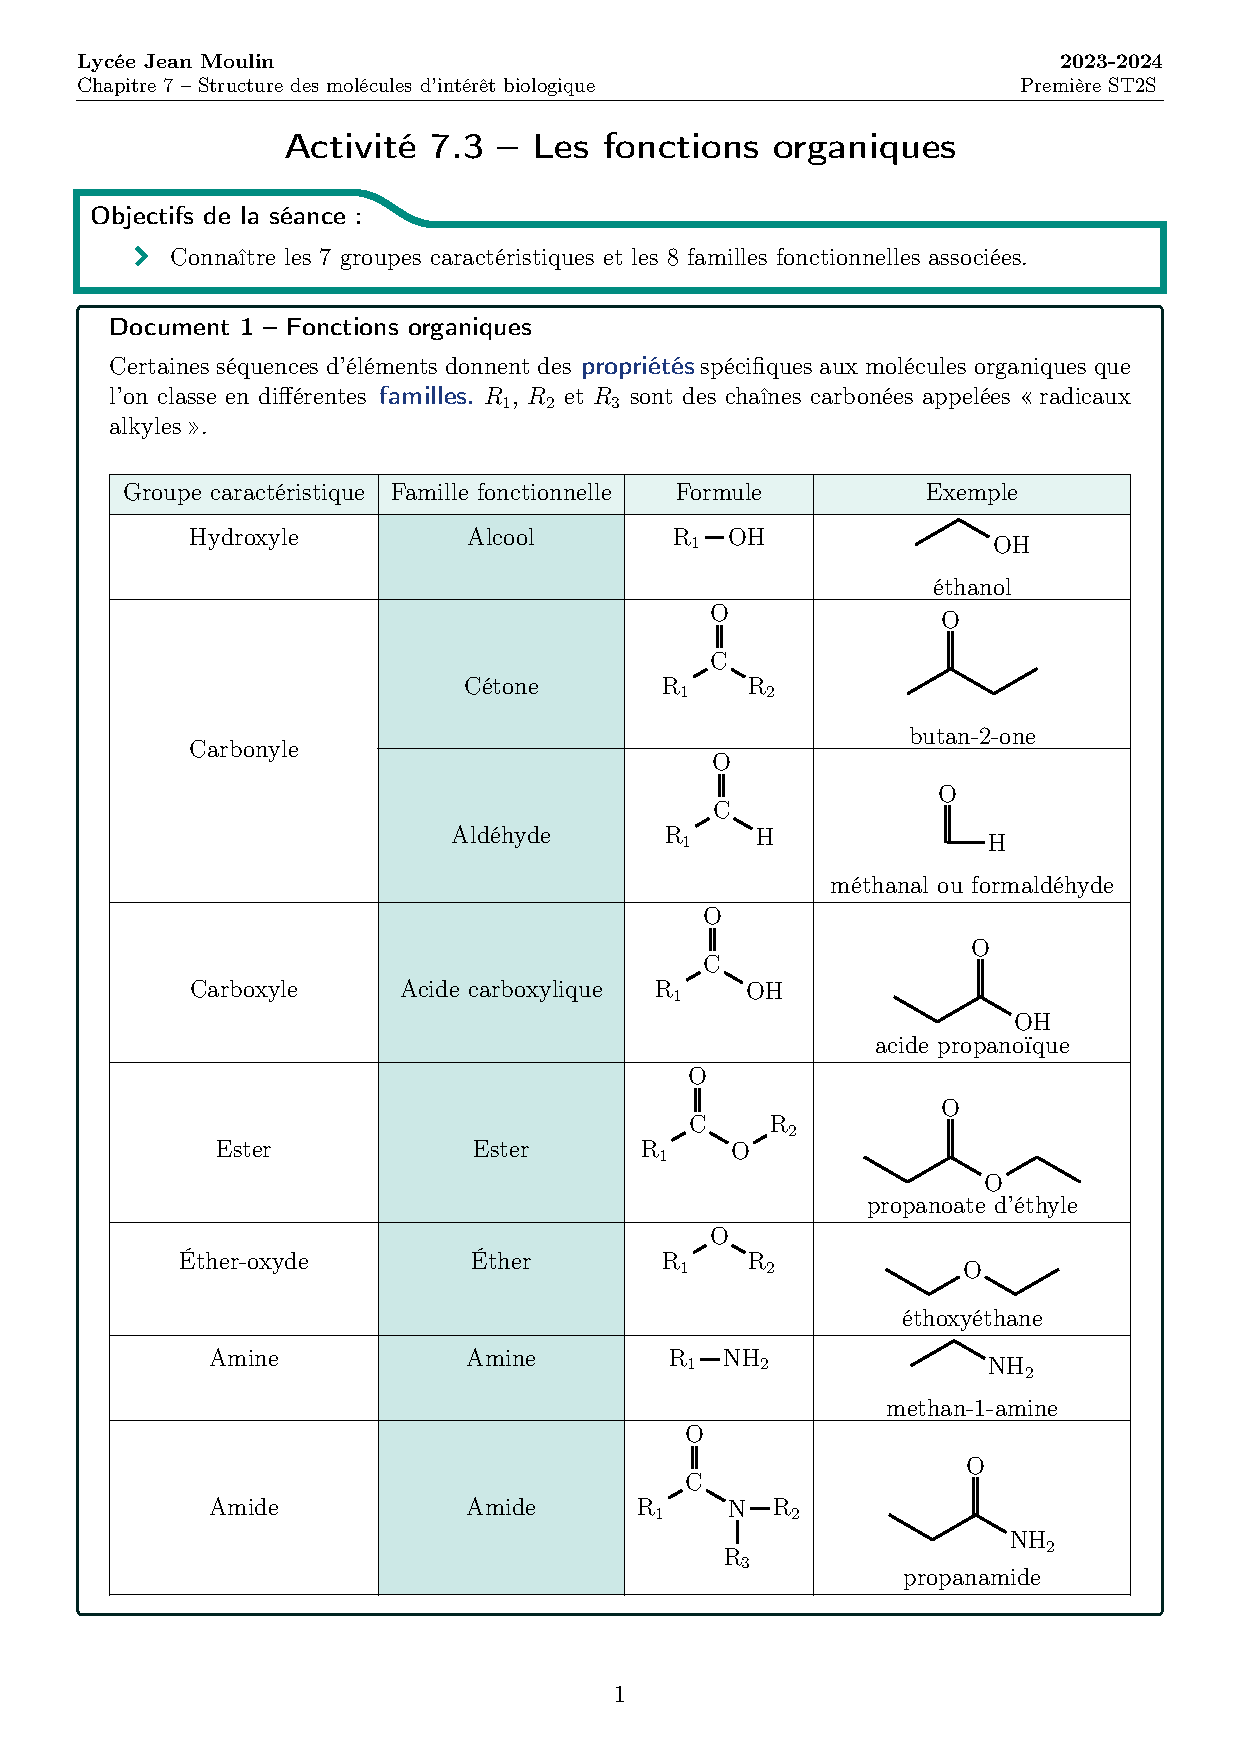
\includepdf{stssPremiere/C7_biomolecules/A7_fonction_orga_tableau}

\begin{doc}{Radicaux alkyle}{doc:A3_radicaux_alkyles}
  \begin{importants}
    Les \important{« radicaux alkyles »,} notés R, sont des morceaux de chaînes carbonées composées de liaisons simples avec des hydrogènes.
  \end{importants}

  \begin{tblr}{
    colspec = {|X[c] |X[c] |X[c] |X[c] |}, hlines,
    row{1} = {couleurPrim!20}
  }
    Méthyle & Éthyle & Propyle \\
    \vAligne{20pt} & & \\
  \end{tblr}
\end{doc}

\question{
  Identifier les fonctions organiques présentes dans les molécules suivantes
  
  \begin{center}
    \begin{tblr}{c c c c c}
      \chemfig{-[1] O -[-1] -[1]} &
      \chemfig{-[1] C (=[3] O) -[-1] OH} &
      \chemfig{-[1] !\ester -[1] -[-1] -[1]} &
      \chemfig{-[1] -[-1] -[1] (=[3] O) -[-1] H} &
      \chemfig{-[1] -[-1] -[1] (=[3] O) -[-1]} \\
      % 
      1 & 2 & 3 & 4 & 5
    \end{tblr}
  \end{center}
  \phantom{bla}
}{}{4}
  % %%%%
\tetePremStssStru

%%%% titre
\numeroActivite{4}
\titreActivite{Nomenclature en chimie organique}

%%%% objectifs
\begin{objectifs}
  \item Savoir nommer des molécules organiques simples.
  \item Savoir reconnaître la fonction principale d'une molécule organique à partir de son nom.
\end{objectifs}

\begin{contexte}
  Il existe des millions de molécules organiques, certaines avec des propriétés similaires.

  \problematique{
    Comment nommer ces molécules selon leur propriétés et leur structures ?
  }
\end{contexte}


\begin{doc}{Principe de la nomenclature}{doc:A4_principe_nomenclature}
  \begin{importants}  
    La \important{nomenclature} est l'ensemble des règles établies pour nommer les molécules organiques.
  \end{importants}
   
  La nomenclature moderne repose sur deux principes :
  \begin{listePoints}
    \item décrire la \important{géométrie} de la molécule nommée ;
    \item indiquer les \important{fonction organiques} présentes dans la molécule.
  \end{listePoints}
\end{doc}

%%
\begin{doc}{Nommer une chaîne carbonée}{doc:A4_chaine_carbonee}
  Toute molécule organique possède au moins une chaîne carbonée.
  Pour nommer une chaîne carbonée, on va associer un \important{préfixe} avec un \important{suffixe}.
  Le suffixe dépend de la fonction organique, mais le préfixe est déterminé par le nombre de carbones qui composent la chaîne.
  \begin{importants}
  \begin{center}
    \begin{tblr}{
      columns = {c}, vlines, hlines,
      row{1} = {couleurPrim!20!},
      column{1} = {couleurPrim!30}
    }
      Nombre de carbone \chemfig{C} 
      & 1 & 2 & 3 & 4 & 5 & 6 \\
      Préfixe
      & meth- & éth- & prop- & but- & pent- & hex- \\
    \end{tblr}
  \end{center}  
  \end{importants}
\end{doc}

%%
\titreSousSection{Règles pour les alcanes, alcènes ou alcynes}

\begin{doc}{Les alcanes}{doc:A4_alcanes}
  \begin{wrapfigure}{r}{0.45\linewidth}   
    \vspace*{-30pt}
    \begin{boite}
      \begin{importants}
        Un \important{hydrocarbure} est une molécule qui ne contient que des éléments carbones et hydrogènes.
      \end{importants}
      \begin{importants}
        Un hydrocarbure est \important{saturé} (en hydrogène) s'il ne comporte que des \important{liaisons simples}. \\
        Si l'hydrocarbure comporte des \important{liaisons doubles} ou \important{triples}, on dit qu'il est \important{insaturé.}
      \end{importants}
      % \vAligne{-38pt}
    \end{boite}
  \end{wrapfigure}
  \phantom{b}\vspace*{-14pt}
  
  \begin{importants}
    Une molécule d'alcane est un \important{hydrocarbure} saturé, composé de \important{liaisons simples}.
  \end{importants}
  Pour nommer un alcane, il faut déterminer la chaîne carbonée la plus longue qui compose la molécule. \\
  On écrit alors le préfixe lié à la longueur de la chaîne et on ajoute le suffixe « \important{-ane} ». \\
  Un alcane a toujours une formule brute de la forme \chemfig{C_{n} H_{2(n + 1)}} (\chemfig{C_4H_{10}} par exemple).
  
  \vspace*{4pt}
  \exemple \chemfig{H_3C - CH_2 - CH_3} trois carbones dans la chaîne, donc prop- + -ane : propane.
\end{doc}

%%%% Question
\question{
  Nommer les molécules suivantes :
  \begin{equation*}  
    \chemfig{H_3C -CH_2 -CH_2 -CH_3} \qq{}
    \chemfig{-[1] -[-1] -[1] -[-1] -[1]} \qq{}
    \chemfig{H -C !\paireH -C !\saturationH}
  \end{equation*}
}{
  Butane, hexane et éthane.
}{1}


%%
\begin{doc}{Les alcènes}{doc:OA_2alcenes}
  \begin{importants}
    Les alcènes sont des hydrocarbures avec au moins une liaison double.
    Le suffixe « -ane », devient « \important{-ène} ».
    On indique le (ou les) numéro de la liaison double avant le suffixe, de sorte que \important{le numéro soit le plus petit possible}.
  \end{importants}
  \exemple \chemfig{H_3C- CH_2 - CH = CH -CH_3} cinq carbones dans la chaîne (pent-) et la liaison double se trouve en position 3 ou 2 (si on compte depuis la droite).
  Donc pent $+$ 2 $+$ ène : but-2-ène.
\end{doc}

%%
\begin{doc}{les alcynes}{doc:A4_alcynes}
  \begin{importants}
    Les alcynes sont des hydrocarbures avec au moins une liaison triple.
    Le suffixe « -ane », devient « \important{-yne} ».
    On indique le (ou les) numéro de la liaison triple avant le suffixe, de sorte que \important{le numéro soit le plus petit possible}, comme pour les alcènes.
  \end{importants}
  \exemple \chemfig{-[1] ~[-1]} : trois carbones dans la chaîne (prop-) et la liaison triple se trouve en position 1.
  Donc prop-1-yne ou propyne (le 1 est implicite).
\end{doc}



%%%%
\titreSousSection{Règles pour les ramifications}

\begin{doc}{Ramification à la chaîne principale}{doc:A4_ramification}
  \begin{importants}  
    Une \important{ramification} est un substituant qui remplace un hydrogène sur la chaîne principale.
  \end{importants}
  Si le substituant est un \important{alkyle} (un hydrocarbure), son nom prend le suffixe « \important{-yl} ».

  \exemples \chemfig{CH_3 -[6]} : méthyl, \chemfig{CH_2 (-[6]) -CH_3} éthyl.
\end{doc}

\begin{doc}{Nommer une ramification}{doc:A4_nom_ramification}
  \begin{importants}
  Pour nommer une molécule contenant des ramifications, il faut :
  \begin{listePoints}
    \item trouver la \important{plus longue chaîne carbonée} pour déterminer son nom.
    \item \important{Numéroter} la chaîne carbonée afin que la ramification ait le numéro le plus \important{petit possible}, comme pour les alcènes ou les alcynes.
    \item Placer le \important{numéro} et le \important{nom} de l'alkyle avant le nom de la chaîne.
  \end{listePoints}
  \end{importants}
  S'il y a plusieurs ramifications, leurs noms sont placés par ordre alphabétique.
\end{doc}

\vspace*{-8pt}
\numeroQuestion
Nommer la molécule suivante :\\[4pt]

\begin{minipage}[T]{0.48\linewidth}
  \centering
  \chemfig{H_3C- CH (-[3]CH_3) - CH (-[-3]CH_2 -CH_3) -CH_3}
\end{minipage}
\begin{minipage}[T]{0.48\linewidth}
  \phantom{b} \dotfill \\[8pt]
  \phantom{b} \dotfill \\[8pt]
  \phantom{b} \dotfill
\end{minipage}

\correction{
  Pour la molécule 1 : la chaîne principale a 4 atomes, donc -butane.
  Deux ramifications sont en position 2 (avec un méthyl) et 3 (avec un éthyl).
  Donc le nom de cette molécule est 3-éthyl-2-méthyl-butane.
}

%%
\titreSousSection{Règles pour les groupes caractéristiques}

\begin{doc}{Groupes caractéristiques}{doc:A4_nom_groupe_carac}
  \vspace*{-4pt}
  \begin{wrapfigure}[5]{r}{0.58\linewidth}
    \vspace*{-30pt}
    \centering
    \begin{tikzpicture}[help lines/.style={thin,draw=black!50}]
      % chaine principale et carbone fonctionnel
      \large
      \node[draw] at (3,3) { \chemfig{
        H_3C-CH-CH_2 -\textcolor{couleurSec}{\textsf{\important{C}}} H-CH_3
        }
      };
      \draw (5, 2.25) node[right] {\important{chaîne principale}};
      \draw[couleurSec] (3.7, 3.7) node[right] {\important{carbone fonctionnel}};
      % Ramification
      \draw[very thick, couleurPrim] (1.51, 2.79) -- (1.51, 2.29);
      \draw[couleurPrim] (2.5, 1.3)  node[left] {\important{ramification}};
      \node[draw, couleurPrim] at (1.8, 2) { \chemfig{CH_3} };
      % Alcool
      \draw[very thick, violet] (4.11, 2.79) -- (4.11, 2.29);
      \draw[violet] (3.6, 1.3)  node[right] {\important{groupe caractéristique}};
      \node[draw, violet] at (4.28, 2){ \chemfig{OH_{}} };
    \end{tikzpicture}
  \end{wrapfigure}
  %
  Pour nommer les molécules contenant des groupes caractéristiques, on utilise les règles décrites dans le tableau ci-dessous, en respectant la priorité des fonctions organiques.
  
  \begin{importants}
    Le \important{carbone fonctionnel} désigne le carbone contenant la fonction de la molécule.
  \end{importants}
  
  Pour les cétones, alcools et amines, le numéro est celui du \important{carbone fonctionnel}, comme pour les ramifications il \important{doit être le plus petit possible}.
  
  ($R_1$) et ($R_2$) représentent les noms des chaînes carbonées auxquels les groupes caractéristiques sont attachées. 

  \vspace*{4pt}
  \begin{tblr}{
    width = \linewidth,
    colspec = {|c |c |c |X |}, hlines,
    column{2,4} = {couleurPrim!20},
    row{1} = {couleurPrim!10},
    rows = {m}, columns = {c}
  }
    Priorité & Famille fonctionnelle & Formule & Nom si prioritaire \\
    %
    1 & Acide carboxylique
    & \chemfig{\textcolor{couleurQuat}{C} !\alkyleG !\cetoneCouleur \textcolor{couleurQuat}{OH}}
    & acide ($R_1$)-oïque \\
    %
    2 & Ester
    & \chemfig{\textcolor{couleurQuat}{C} !\alkyleG !\cetoneCouleur \textcolor{couleurQuat}{O} -[1] R_2}
    & ($R_1$)-oate de ($R_2$)-yle \\
    %
    3 & Amide
    & \chemfig{\textcolor{couleurQuat}{C} !\alkyleG !\cetoneCouleur \textcolor{couleurQuat}{N} H_2}
    & ($R_1$)-amide \\
    %
    4 & Aldéhyde
    & \chemfig{\textcolor{couleurQuat}{C} !\alkyleG !\cetoneCouleur \textcolor{couleurQuat}{H}}
    & ($R_1$)-al \\
    %
    5 & Cétone
    & \chemfig{\textcolor{couleurQuat}{C} !\alkyleG !\cetoneCouleur R_2}
    & ($R_1$)-(numéro)-one \\
    %
    6 & Alcool
    & \chemfig{R_1 - \textcolor{couleurQuat}{OH}}
    & ($R_1$)-(numéro)-ol \\
    %
    7 & Amine & \chemfig{R_1 - \textcolor{couleurQuat}{NH_2}}
    & ($R_1$)-(numéro)-amine \\
    %
    8 & Éther
    & \chemfig{R_1 -[1,,,,couleurQuat] \textcolor{couleurQuat}{O} -[-1,,,,couleurQuat] R_2}
    & ($R_1$)-oxy-($R_2$) \\
  \end{tblr}
\end{doc}

\question{
  Nommer la molécule du document~\ref{doc:A4_nom_groupe_carac}.
}{
  4-méthyl-pent-2-ol
}{1}
  % %%%%
\tetePremStssStru

%%%% titre
\numeroActivite{5}
\titreActivite{Les glucides}

\begin{objectifs}
  \item Étudier la structure des glucides.
  \item Comprendre la différence entre un sucre rapide et un sucre lent.
\end{objectifs}

\begin{contexte}
  Les glucides sont une part essentielle de notre alimentation.
  Tous les glucides que nous ingérons sont transformés en glucose au cours de la digestion,
  qui peut ensuite être utilisé par nos cellules.

  \problematique{
    Quelle est la structure des glucides ?
  }
\end{contexte}



%%%%%
\begin{doc}{Sucres rapides et sucres lents}{doc:A5_sucre_rapide_lent}
  \begin{importants}
    On classe les glucides en deux catégories :
    \begin{listePoints}
      \item les \important{sucres rapides,} qui sont des molécules simples et facilement digérés ;
      \item les \important{sucres lents,} qui sont composés de plusieurs sucres rapides liés entre eux.  
    \end{listePoints}
    L'assimilation des sucres lents par l'organisme est lente et permet un apport régulier en sucre rapide pendant toute la digestion.
  \end{importants}

  On trouve des sucres rapides dans les fruits, le miel, la farine blanche, le riz blanc et la plupart des sodas et sucreries.
  Les sucres lents se trouvent dans les féculents (pomme de terre, maïs, blé, etc.), les légumineuses (haricot rouge, pois chiche, etc.), la farine complète ou le riz complet.
\end{doc}

\begin{doc}{Le glucose et le fructose sous forme linéaire et cyclique}{doc:A5_glucose_fructose}
  \begin{multicols}{2}
  \begin{center}
    %% glucose linéaire
    \chemfig{
      HO -C (-H)
        (-[3] C (-H) (-[6] HO)
          (-[3] C (-[5]H) =[1] O)
        ) % aldehyde et alcool
      -[-3] C (-H) (-[6] HO)
      -[-3] C (-H) (-[6] HO)
      -[-3] C (-H) (-[6] HO)
      -[-3] H
    }
    \phantom{b}
    % glucose hamworth
    \chemfig[cram width=2pt, atom sep=2.5em]{!\glucoseHamw} \\[4pt]
    Glucose

    %% fructose linéaire
    \chemfig{
      HO -C (-H)
        (-[3] C (=O)
          (-[3] C (-[3]H) (-[6]H) -OH)
        ) % cétone et alcool
      -[-3] C (-H) (-[6] HO)
      -[-3] C (-H) (-[6] HO)
      -[-3] C (-H) (-[6] HO)
      -[-3] H
    }
    \phantom{b}
    % fructose hamworth
    \chemfig[cram width=2pt, atom sep=2.5em]{!\fructoseHamw} \\[4pt]
    Fructose
  \end{center}
  \end{multicols}
\end{doc}

\question{
  À partir de la forme linéaire du glucose et du fructose, entourer et nommer les fonctions organiques présentes dans ces deux molécules.
}{}{4}

\newpage
\question{
  Donner la formule brute du glucose et la formule brute du fructose.
  Ces molécules sont-elles isomères ?
}{}{2}


\begin{doc}{Une partie de l'amidon}{doc:A5_amidon}
  \begin{center}
    \chemfig[cram width=2pt, atom sep=2.5em]{
      ...\phantom{B}-[-1] !\amylopectineHamw
      !\amylopectineHamw O -[-3]
      !\amylopectineCentraleHamw
      !\amylopectineHamw !\amylopectineHamw O -[1]...
    } \\[8pt]
  
    \important{Amylopectine,} molécule composant l'amidon
  \end{center}
\end{doc}

\begin{doc}{Le test de Fehling}{doc:A5_test_fehling}
  Le test à la liqueur de Fehling permet de déterminer si une solution contient des fonctions aldéhydes.

  \begin{protocole}
    \item Mélanger \qty{0,5}{\ml} de liqueur de Fehling avec \qty{1}{\ml} de solution à tester dans un tube à essais.
    \item Chauffer le tube à essais aec le mélange quelques minutes dans un bain-marie.
  \end{protocole}

  \begin{center}

    \begin{tblr}{
      colspec = {X[l] X[l] X[l]}, hlines, vlines,
      column{1} = {couleurPrim!10},
      row{1} = {couleurPrim!20}
    }
      &
      Présence d'une fonction aldéhyde &
      Présence d'une fonction cétone \\
      %
      Observation dans le tube à essais &
      Apparition d'un précipité rouge brique &
      La solution reste bleue. \\
    \end{tblr}
  \end{center}
\end{doc}

\question{
  Indiquer, en justifiant, la catégorie de glucides dans laquelle se trouvent le glucose, le fructose et l'amidon.
}{}{3}

\mesure
Mettre en oeuvre un protocole expérimental permettant de distinguer des solutions de glucose et de fructose.
  % %%%%
\tetePremStssStru

%%%% titre
\vspace*{-36pt}
\numeroActivite{6}
\titreActivite{Les lipides}

\begin{objectifs}
  \item Étudier la structure des lipides.
  \item Comprendre la composition d'un triglycéride.
\end{objectifs}

\begin{contexte}
  Les lipides sont les molécules composants les matières grasses et ne sont pas solubles dans l'eau.
  Ils entrent dans la constitution de la membranes de nos cellules et forment aussi une importante réserves d'énergie dans notre organisme.

  \problematique{
    Quelle est la structure des lipides ?
  }
\end{contexte}



%%%%%
\begin{doc}{Structure d'un lipide}{doc:A6_structure_lipide}
  \begin{importants}
    Les lipides constituent la matière grasse du vivant.
    Les lipides sont des molécules \important{hydrophobes,} qui ne se mélangent pas avec l'eau.
  \end{importants}
  Les lipides peuvent se trouver sous formes solide (cire, graisse), ou liquide (huile).
  
  On va étudier deux types de lipides : les acides gras et les triglycérides.
\end{doc}

\begin{doc}{Les acides gras}{doc:A6_acide_gras}
  \begin{importants}
    Les \important{acides gras} sont des \important{acides carboxyliques} qui possèdent une longue chaîne carbonée sans ramification.
    Les acides gras peuvent être 
    \begin{listePoints}
      \item \important{saturés} (en hydrogène) si la chaîne carbonée ne comporte que des liaisons carbone-carbone simples ;
      \item \important{insaturés} si la chaîne carbonée comporte au moins une liaison carbone-carbone double.
    \end{listePoints}
  \end{importants}
  
  \begin{multicols}{2}
    \centering
    \chemname[8pt]{
      {\small
        \chemfig[atom sep = 1.4em]{OH-[1]!\palmitique}
      }
    }{
      Acide palmitique, un acide gras \important{saturé.}
    }

    \chemname[8pt]{
      {\small
        \chemfig[atom sep = 1.4em]{[:30]HO-!\trioleique}
      }
    }{
      Acide oléique, un acide gras \important{insaturé.}
    }
  \end{multicols}

  Les acides gras saturés ont une formule brute de la forme \bruteCHO{n}{2n}{2}.

  Dans le cadre d'une alimentation saine, il faut limiter les acides gras saturés et privilégier les lipides riches en acides gras insaturés.
\end{doc}

\begin{doc}{Quelques acides gras et leurs sources}{doc:A6_sources_acides_gras}
  \begin{tblr}{
    colspec = {X[l] X[l] X[l] X[l] X[l]}, hlines, vlines,
    column{1} = {couleurPrim!20, font=\bfseries},
    row{2} = {c},
  }
    Acide gras &
    Acide stéarique &
    Acide palmitique &
    Acide oléique &
    Acide $\alpha$-linolénique \\
    %
    Formule brute &
    \bruteCHO{18}{36}{2} &
    \bruteCHO{16}{32}{2} &
    \bruteCHO{18}{34}{2} &
    \bruteCHO{18}{32}{2} \\
    %
    Sources dans l'alimentation &
    Boeuf, mouton, porc, beurre &
    Huile de palme, huile de coco &
    Olive, amande, avocat, noisette &
    Tournesol, colza, maïs, cacahuète
  \end{tblr}
\end{doc}

\question{
  Entourer et nommer les fonctions organiques qui sont présentes dans l'acide palmitique et l'acide oléique.
}{}{2}

\question{
  Indiquer si l'acide stéarique et l'acide oléique sont saturés ou insaturés.
}{}{2}


%%%%
\begin{doc}{Les triglycérides}{doc:A6_triglycerides}
  \vspace*{-18pt}
  \begin{wrapfigure}[2]{r}{0.3\linewidth}
    \centering
    \chemfig{CH_2 (-[3]OH) -CH (-[3]OH) -CH_2(-[3]OH)}
  
    Glycérol
  \end{wrapfigure}
  \vphantom{b}
  \begin{importants}
    Les \important{triglycérides} sont des \important{triester} composés d'un \important{glycérol} et de trois \important{acides gras} (pas forcément trois fois le même).
  \end{importants}

  \begin{center}
    {\small
      \chemfig[atom sep = 1.25em]{[:-60]!\tripalmitine}
      \qq{} ou \qq{}
      \chemfig[atom sep = 1.75em]{
        H C (!\teteAcideDev C_{15} H_{31}) 
        (-[3,1.7,2,2] H_2C (!\teteAcideDev C_{15} H_{31}))
        -[-3,1.7,2,2] H_2 C (!\teteAcideDev C_{15} H_{31})
      } \\[8pt]
    }
    \legende{
      Tripalmitine, triglycéride composé d'un glycérol et de trois acide palmitique
    }
 \end{center}

  \begin{wrapfigure}{l}{0.45\linewidth} 
    \centering
    \small{
      \chemfig[atom sep = 1.25em]{
        (-[::150] -[::60] O-[::-60] !\trioleique)  % haut
        (-[::-90] -[::60] O-[::30] !\trilinoleique) % bas
        -[::30] O-[::60] !\trilinolenique % centre
      }
    }
  \end{wrapfigure}
 
  \textcolor{couleurPrim}{\faArrowLeft} \; 
  Triglycéride composé de trois acides gras différents.
    
  \begin{importants}
    Un triglycéride est \important{insaturé} s'il comporte \important{au moins un} acide gras insaturé.
  \end{importants}
  
  Les triglycérides compose la majorité des lipides.

  \begin{doc}{Acide gras et cholestérol}{doc:A6_sante}
    Les acides gras saturés ou les triglycérides saturés augmentent la présence de cholestérol dans le sang.

    S'il y a trop de cholestérol dans le sang, on parle \important{d'hypercholestérolémie,} ce qui entraine la formation de plaques graisseuses sur les parois sanguines.
    Ce rétrécissement des vaisseaux sanguins gêne la circulation sanguine dans le corps, ce qui peut mener à des accidents cardiovasculaires.
  \end{doc}
\end{doc}

\numeroQuestion
Repérer et entourer les fonctions ester dans les triglycérides du document~\ref{doc:A6_triglycerides}.

\question{
  Quels aliments faut-il éviter si on souffre d'hypercholestérolémie ?
}{}{2}


%%%% DANS UNE ACTIVITE SUR LA POLARITE DE L'EAU
% \begin{doc}{Micelles et membrane cellulaire}{doc:A6_micelle_membrane}
%   La structure des molécules de lipides mène à la formation de structure particulière dans de l'eau liquide.
%   Les queue hydrophobe étant repoussée par les molécules d'eau, elles vont s'agglomérer et former des structures ou les queues sont isolées de l'eau environnante : \important{les micelles.}
  
%   Des exemples de micelles sont \important{les couches bi-lipidique,} composée de deux couches de lipides avec les têtes hydrophile orientée vers l'extérieur, ce qui permet à leur queue hydrophobes de ne pas rentrer en contact avec de l'eau. 
%   Les interactions électrostatiques entre les différentes parties de la membrane la pousse à former une sphère (comme une bulle de savon), avec un extérieur et un intérieur : c'est la base \important{d'une membrane cellulaire.}

%   Les membranes cellulaire sont plus complexe qu'une simple couche bi-lipidique : elles sont aussi composées de \important{protéines}, qui permettent de renforcer la structure de la membrane cellulaire et de contrôler ce qui sort et ce qui entre de la cellule.

%   TODO : FIGURE MICELLE ET MEMBRANE
% \end{doc}
  % %%%%
\tetePremStssStru

%%%% titre
\vspace*{-36pt}
\numeroActivite{7}
\titreActivite{Les protéines}

\begin{objectifs}
  \item Étudier la structure des protéines et des acides aminés.
\end{objectifs}

\begin{contexte}
  Les protéines sont des molécules complexes qui permettent à nos organismes de fonctionner en remplissant en ensemble varié de rôles en son sein.

  \problematique{
    Quelle est la structure des protéines ?
  }
\end{contexte}



%%%%%
\begin{doc}{Acides $\mathbf{\alpha}$-aminés}{doc:A7_acides_amines}
  \begin{wrapfigure}{r}{0.3\linewidth}
    \centering
    \vspace*{-14pt}
    \chemfig{CH_3- CH (-[-3] NH_2) - C (=[1.5] O) -[-1.5] OH} \\[4pt]
    Molécule d'alanine \\[8pt]

    \chemfig{NH_2- CH_2- C (=[1.5] O) -[-1.5] OH} \\[4pt]
    Molécule de glycine
  \end{wrapfigure}
  \phantom{b}\vspace*{-16pt}
  
  \begin{importants}
    Les \important{acides $\alpha$-aminés} sont des molécules composées d'une fonction \important{acide carboxylique} et d'une fonction \important{amine} (d'où leur nom).
    Ces deux fonctions sont liées au même carbone fonctionnel.
  \end{importants}
  
  Sur Terre, les organismes vivants synthétisent et utilisent 20 acides aminés.
  Parmi ces 20 acides aminés, 8 ne sont pas synthétisés par le corps humain, on dit que ce sont des \important{acides aminés essentiels,} qui doivent être apportés par une alimentation équilibrée.
\end{doc}

\begin{doc}{Quelques acides $\alpha$-aminés essentiels}{doc:A7_aa_essentiels}
  \centering
  \begin{tblr}{
    columns = {c},
  }
    \chemfig{H_2N -[1] (-[3] (-[1]) -[5] -[3]) -[-1] !\carboxyle} &
    \chemfig{H_2N -[1] (-[3] -[5] (-[-5]) -[3]) -[-1] !\carboxyle} &
    \chemfig{H_2N -[1] (-[3] -[5] -[3] S -[5]) -[-1] !\carboxyle} &
    \chemfig{H_2N -[1] (-[3] (-[1]) -[5]) -[-1] !\carboxyle} \\
    %
    Isoleucine & Leucine & Methionine & Valine \\
    %
  \end{tblr}
\end{doc}

\question{
  Justifier que l'isoleucine est bien un acide $\alpha$-aminé.
}{}{2}

\numeroQuestion Entourer les groupes fonctionnels de la leucine et de la méthionine.


\begin{doc}{Séquence de 3 acides $\alpha$-aminés dans l'insuline humaine}{doc:A7_insuline_aa}
  \begin{center}
    \chemfig{
      NH_2 - CH_2
      -C (=[3] O) -NH
      %
      -CH (-[-3] CH (-[-5] CH_2 -[-3]CH_3) -[-1]CH_2)
      -C (=[3] O) -NH
      %
      -CH (-[3] CH (-[5] CH_3) -[1]CH_2)
      -C (=[-3] O) -[1]OH
    }
  \end{center}
\end{doc}

%%%%
\begin{doc}{Les protéines}{doc:A7_proteines}
  Deux acides aminés peuvent se lier quand un groupe carboxyle réagit avec un groupe amine, c'est la \important{liaison peptidique.}
  
  \begin{center}
    \chemfig{R- C (=[3] O) -OH} +   
    \chemfig{N (-[6] H) (-[-3] H) -R'}
    \reaction
    \chemfig{R- C (=[3] O) -N (-[-3] H) -R'} +
    \chemfig{H_2O}
  \end{center}
  \vspace*{-4pt}

  Comme tous les acides aminés possèdent un \important{groupe amine} et un \important{groupe carboxyle}, cette réaction peut se répéter pour former une chaîne d'acides aminés appelée \important{polypeptide}.

  \begin{importants}
    Une \important{protéine} est un polypeptide qui s'est replié sur lui même.
    Ce repliement lui donne une structure tridimensionnelle unique, qui lui confère une \important{fonction biologique} particulière.
  \end{importants}
  \begin{center}
    \image{1}{images/proteines/structure_proteines}
  \end{center}
\end{doc}


\begin{doc}{Rôle des protéines dans l'organisme}{doc:A7_proteine_organisme}
  Les protéines sont omniprésentes dans tous les organismes vivants : elles sont les petites ouvrière qui en assure le bon fonctionnement.
  
  Elles remplissent un ensemble varié de fonctions, de l'échelle d'une cellule (réplication ou transcription de l'ADN, fabrication de protéines, structure de la cellule, etc.), à l'échelle du corps entier (transport d'oxygène, transmission d'information, structure des muscles, etc.).

  Par exemple, l'hémoglobine permet de transporter le dioxygène des poumons jusqu'aux cellules.
  L'insuline permet de signaler aux cellules de capter le glucose qui circule dans le sang.
  Des enzymes digestives permettent de digérer les glucides complexes pour les transformer en glucose.

  Contrairement aux glucides et aux lipides, les protéines sont dénaturées en \important{urée dans le foie} une fois utilisées.
  L'urée est ensuite évacuée par les urines.
\end{doc}

\question{
  Entourer et nommer le groupe formé au cours de la liaison peptidique.
}{}{1}

\question{
  Identifier les 3 acides aminés présents dans la séquence de l'insuline présentée dans le document~\ref{doc:A7_insuline_aa},
  en vous aidant des documents~\ref{doc:A7_acides_amines} et~\ref{doc:A7_aa_essentiels}.
}{}{2}
  % %%%%
\tetePremStssStru

%%%% titre
\numeroActivite{8}
\titreActivite{Les vitamines}

\begin{objectifs}
  \item Comprendre ce que c'est qu'une vitamine.
  \item Étudier un exemple de vitamine : la vitamine C.
\end{objectifs}

\begin{contexte}
  Contrairement aux glucides, lipides et protéines, les vitamines n'ont pas de structures particulière distinguable.
  Les vitamines sont simplement des molécules essentielles au bon fonctionnement du corps humain.
  On va étudier un exemple de vitamine : la vitamine C.

  \problematique{
    Quelle sont les propriétés de la vitamine C ?
  }
\end{contexte}



%%%%%
\begin{doc}{La vitamine C : l'acide ascorbique}{doc:A8_vitamineC}
  \begin{center}
    \chemfig{
      HO -[-1] -[1] (-[3] OH) -[-1]
     *5(-(-OH) =(-OH) -(=O)-O-) % cycle
    }\\[4pt]
    
    \legende{Acide ascorbique, de formule brute \bruteCHO{6}{8}{6}}
  \end{center}
  La vitamine C est une molécule, l'acide ascorbique. 
  Elle remplit plusieurs fonctions dans l'organisme :
  \begin{listePoints}
    \item défense contre les infections virales ou bactériennes ;
    \item protection contre le vieillissement des cellules grâce à son action anti-oxydante ;
    \item protection de la paroi des vaisseaux sanguins ;
    \item meilleur assimilation du fer ;
    \item formation du collagène ;
    \item cicatrisation des plaies ; etc.
  \end{listePoints}
\end{doc}

\question{
  Recopier la molécule composant la vitamine C, puis entourer et nommer les fonctions organiques présentes.
}{}{8}

\begin{doc}{Mise en évidence des propriétés de la vitamine C}{doc:A8_test_vitamine}
  Le permanganate de potassium est une \important{solution oxydante.}
  En milieu acide et en présence de fonction alcool, le permanganate de potassium se décolore (la solution passe de violette à transparente).

  Le protocole suivant est réalisé :
  \begin{protocole}
    \item un comprimé de vitamine C est dissout dans de l'eau ;
    \item le pH de cette solution est mesuré, on trouve un pH de 4 ;
    \item \qty{2}{\ml} de permanganate de potassium est versé dans un tube à essai ;
    \item quelques gouttes de solution contenant de la vitamine C sont versées dans le tube à essai ;
    \item on observe alors une décoloration de la solution de permanganate.
  \end{protocole}
\end{doc}

\question{
  La solution contenant la vitamine C est-elle acide ? Justifier.
}{}{2}

\question{
  Quelle fonction organique de la vitamine C le test réalisé dans le document~\ref{doc:A8_test_vitamine} permet d'identifier ?
}{}{3}

\question{
  Quelle propriété de la vitamine C est mise en évidence par le test réalisé avec le permanganate de potassium ?
}{}{3}


\begin{doc}{Pourquoi il faut consommer de la vitamine C}{doc:A8_source_vitamine_C}
  \QRCode{https://www.anses.fr/fr/content/vitamine-c}
  
  « La vitamine C permet de consolider les fibres de collagène, constitutives du tissu conjonctif qui soutient les cellules et structure ainsi les autres tissus.
  Elle intervient dans la synthèse de molécules impliquées dans la transmission nerveuse (ex. noradrénaline).
  Elle assure un rôle protecteur des tissus en captant les substances oxydantes.
  Enfin, elle facilite l’absorption du fer non héminique (présent dans les aliments d’origine végétale comme les légumineuses ou les noix). 
  \medskip
  
  Les besoins en vitamine C peuvent être couverts en consommant des fruits [frais] tels que les cassis et les agrumes, et des légumes, en particulier le persil et les poivrons.
  \medskip

  La pathologie spécifique liée à la carence en vitamine C est le scorbut.
  Elle se manifeste par un saignement des gencives, un déchaussement des dents ou encore des douleurs des articulations. »

  \begin{flushright}
    D'après \url{https://www.anses.fr/fr/content/vitamine-c}
  \end{flushright}
\end{doc}

\question{
  Quelles sont les sources de vitamine C ?
}{}{1}
  %% Organisme et biomolécules
  % %%%%
\tetePremStssBiom

%%%% titre
\vspace*{-30pt}
\numeroActivite{1}
\titreActivite{Solubilité des espèces dans l'eau}


%%%% objectifs
\begin{objectifs}
  \item Comprendre la notion de liaison polaire.
  \item Comprendre la polarité de la molécule d'eau et la liaison hydrogène.
  \item Comprendre le lien entre liaison hydrogène et solubilité.
\end{objectifs}

\begin{contexte}
  En préparant un gâteau avec du caramel, Medhi remarque que le sucre est soluble dans l'eau, mais que l'huile n'est pas soluble dans l'eau.
  
  \problematique{
    Comment expliquer que certaines espèces chimiques sont plus solubles que d'autres dans l'eau liquide ?
  }
\end{contexte}


%%%% docs
\begin{doc}{Liaison polaire}{doc:A1_liaison_polaire}
  \begin{wrapfigure}[6]{r}{0.56\linewidth}
    \centering
    \vspace*{-20pt}
    \tableauPeriodique[1.9][1.9]{
      \node[name=H,               elec4] {\elementElectroneg{H} {2,20}}; % 1 -IA
      \node[name=Li, below of=H,  elec1] {\elementElectroneg{Li}{0,98}};
      \node[name=Na, below of=Li, elec1] {\elementElectroneg{Na}{0,93}};
      \node[name=Be, right of=Li, elec3] {\elementElectroneg{Be}{1,57}}; % 2 -IIA
      \node[name=Mg, below of=Be, elec2] {\elementElectroneg{Mg}{1,31}};
      \node[name=B,  right of=Be, elec4] {\elementElectroneg{B} {2,04}}; % 13 -IIIA
      \node[name=Al, below of=B,  elec3] {\elementElectroneg{Al}{1,61}};
      \node[name=C,  right of=B,  elec5] {\elementElectroneg{C} {2,50}}; % 14 -IVA
      \node[name=Si, below of=C,  elec4] {\elementElectroneg{Si}{1,90}};
      \node[name=N,  right of=C,  elec6] {\elementElectroneg{N} {3,04}}; % 15 - VA
      \node[name=P,  below of=N,  elec4] {\elementElectroneg{P} {2,19}};
      \node[name=O,  right of=N,  elec7] {\elementElectroneg{O} {3,44}}; % 16 -VIA
      \node[name=S,  below of=O,  elec5] {\elementElectroneg{S} {2,58}};
      \node[name=F,  right of=O,  elec8] {\elementElectroneg{F} {3,98}}; %17 -VIIA
      \node[name=Cl, below of=F,  elec7] {\elementElectroneg{Cl}{3,16}};
    }
    
    \legende{Électronégativité de quelques éléments chimiques}
  \end{wrapfigure}
  \phantom{b}\vspace*{-20pt}
    
  \begin{importants}
    Une \important{liaison covalente} entre deux éléments dans une molécule est \important{polaire} si la charge des électrons mis en commun est dissymétrique entre les deux éléments.
  \end{importants}
  L'attirance des électrons par un élément dépend de son \important{électronégativité,} notée $\chi$ (« ki »).
  Plus l'électronégativité d'un élément est forte, plus il attire les électrons.

  Si on prend \chemfig{O} et \chemfig{H}, on voit qu'il y a une forte différence d'électronégativité ($\chi(O) - \chi(H) > 0,4$), ce qui indique que l'électron sera plus proche de l'oxygène que de l'hydrogène, la liaison \chemfig{O-H} est \important{polaire.}

  \begin{importants}  
    Une liaison polaire implique que la molécule est légèrement chargée électriquement aux extrémité de la liaisons, avec une \important{charge négative} du côté de l'élément le plus électronégatif et une \important{charge positive} du côté de l'élément le moins électronégatif.
  \end{importants}
\end{doc}


\begin{doc}{La molécule H$_2$O}{doc:A1_molecule_eau} 
  \begin{wrapfigure}[3]{l}{0.25\linewidth}
    \centering
    \vspace*{-22pt}
    \image{1}{images/organique/eau_polarite}
  \end{wrapfigure}
  \phantom{b}\vspace*{-20pt}
    
  \begin{importants}
    L'eau est une molécule \important{polaire,} car 
    \begin{listePoints}
      \item la liaison \chemfig{O-H} est une liaison polaire ;
      \item les charge $\delta^+$ et $\delta^-$ n'ont pas le même centre.
    \end{listePoints}
  \end{importants}

  Autour de l'oxygène se trouve une zone chargée négativement de charge $2\delta^-$.
  Autour des deux hydrogènes se trouve deux zones chargées positivement de charge $\delta^+$.  
  Ici $\delta$ est un nombre compris entre $0$ et $e$ la charge élémentaire.
\end{doc}

\begin{doc}{Liaison hydrogène}{doc:A1_liaison_hydrogene}
  \begin{importants}
    La \important{liaison hydrogène} est une liaison électrostatique entre deux molécules polaires.
  \end{importants}
  Comme les deux bouts opposés d'un aimant, les charge + et - s'attirent mutuellement.
  Contrairement aux liaisons covalentes, les liaisons hydrogènes sont représentées en pointillés.

  \begin{importants}  
    Pour les molécules du vivant, les liaisons hydrogène se forment quasiment toujours avec des groupes hydroxyle \chemfig{HO-C...} ou des groupe carbo \chemfig{O=C...}.
  \end{importants}
  C'est parce que l'électronégativité du carbone et de l'oxygène sont différentes
  ($\chi(O) - \chi(C) > 0,4$),
  alors que les électronégativités du carbone, de l'hydrogène et de l'azote sont similaires.
\end{doc}

\begin{doc}{Solubilité}{doc:A1_solubilité}
  \begin{listePoints}
    \item Un solvant est \important{polaire} s'il est composé de molécules polaires : l'eau est un solvant polaire.
    \item Un solvant est \important{apolaire} s'il n'est pas composé de molécules polaires : l'huile est un solvant apolaire.
  \end{listePoints}
  Les solides polaires et ioniques se dissolvent facilement dans les solvants polaires, car des liaisons hydrogènes se forment entre les éléments du solide et les molécules du solvant, ce qui le dissout.

  Les solvants apolaires et polaires ne se mélangent pas.
\end{doc}

\begin{doc}{Glucose et oléine}{doc:A1_glucose_oleine}
  \begin{multicols}{2}
    \centering
    %% glucose linéaire
    {\small
      \chemfig[atom sep = 1.5em]{
         HO -[6] (-[-4] (-[6] HO) -[-2] -[-4] HO) -[4] (-[6] HO) -[2] (-OH) -[4] (=[6] O) -[2] H
      }
    } \\[6pt]
    \legende{Molécule de glucose}

    {\small
      \chemfig[atom sep = 2.0em]{
        H C (!\teteAcideDev C_{17} H_{33}) 
        (-[3,1.7,2,2] H_2C (!\teteAcideDev C_{17} H_{33}))
        -[-3,1.7,2,2] H_2 C (!\teteAcideDev C_{17} H_{33})
      }
    } \\[6pt]
    \legende{Molécule d'oléine}
    %
  \end{multicols}
\end{doc}

\question{
  En s'aidant de l'exemple donné avec la molécule d'eau, montrer que la molécule de glucose est polaire.
}{}{2}

\question{
  Est-ce que la trioléine, qui compose l'huile d'olive, est polaire ?
}{}{1}

\question{
  Expliquer pourquoi le sucre mélange avec l'eau, mais pas l'huile d'olive.
}{}{2}


\begin{doc}{Stockage des nutriments}{doc:A1_stockage}
  La polarité d'une molécule va avoir un impact sur la façon dont elle peut être stockée dans l'organisme.
  Par exemple, les vitamines apolaires peuvent être stockée dans les graisses (elles aussi apolaires), ce qui permet de constituer des réserves, alors que les vitamines polaires vont être dissoutes dans le sang et évacuée par les urines.
\end{doc}


  %%%% Seconde
  % %%%%
\teteSndMeth

%%%% titre
\numeroActivite{1}
\vspace*{-36pt}
\titreActivite{Notation scientifique et unités}

% \begin{objectifs}
%   \item Revoir les puissances de 10 et la notation scientifique
% \end{objectifs}

%%%%
\vspace*{-20pt}
\titreSection{Rappels sur les puissance de 10}
\vspace*{-8pt}

%%
\begin{doc}{Les puissances de 10}{doc:A1_puissance_10}
  Les puissances indiquent qu'on va répéter une multiplication ($2^3 = 2 \times 2 \times 2 = 8$).
  
  Pour lire les puissances de 10, il suffit de suivre deux règles simple
  \begin{importants}
    \pointCyan Écrire le nombre $10^a$ (avec $a = 0, 1, 2, 3, \ldots$), revient à écrire ``$1$'' suivi de $a = 0, 1, 2, 3, \ldots$ zéros. \\
    \exemple \num{e3} = \texteTrou[0.2]{\num{1000}}

    \pointCyan Écrire le nombre $10^{-a}$ (avec $a = 1, 2, 3, \ldots$), revient à écrire ``$0,$'' suivi de $a - 1 = 0, 1, 2, \ldots$ zéros et d'un $1$. \\
    \exemple \num{e-2} = \texteTrou[0.2]{\num{0,01}}
  \end{importants}
\end{doc}


\numeroQuestion Écrire les nombres correspondant aux puissances de 10 suivantes : \\
$\num{e2}  =$ \texteTrou[0.1]{\num{100}} \qq{}
$\num{e5}  =$ \texteTrou[0.2]{\num{100000}} \qq{}
$\num{e-3} =$ \texteTrou[0.1]{\num{0,001}} \qq{}
$\num{e-1} =$ \texteTrou[0.1]{\num{0,1}}

\numeroQuestion Écrire les nombres suivants comme le produit d'un nombre compris entre 0 et 9 et d'une puissance de 10 \exemple \num{600} = \num{6,00e2} :
\begin{multicols}{2}
  \begin{listePoints}
    \item \num{100000}  = \texteTrouLignes{\num{1e5}\\}
    \item \num{1}       = \texteTrouLignes{\num{1e0}\\}
    \item \num{9000000} = \texteTrouLignes{\num{9e6}}
    \item \num{0,1}     = \texteTrouLignes{\num{1e-1}\\}
    \item \num{0,0006}  = \texteTrouLignes{\num{1e-4}\\}
    \item \num{0,00705} = \texteTrouLignes{\num{7,05e-3}}
  \end{listePoints}
\end{multicols}


%%
\pasCorrection{\vspace*{-8pt}}
\begin{doc}{Règles de calculs}{doc:A1_calcul_puissance_10}
  Il y a deux règles de calculs à connaître pour les puissances de 10
  \begin{importants}
    \pointCyan $10^a \times 10^b = 10^{a + b}$ \\   
    \pointCyan $10^{-a} = \dfrac{1}{10^a}$
  \end{importants}
\end{doc}


\numeroQuestion Réaliser les calculs suivants :
\begin{multicols}{2}
  \begin{listePoints}
    \item $10^2 \times 10^1 =$ \texteTrouLignes{$10^{2 + 1} = 10^3 = 1000$\\}
    \item $10^4 \times 10^{-3} =$ \texteTrouLignes{$10^{4 - 3} = 10^1 = 10$}
    \item $10^{-2} \times 10^{-3} =$ \texteTrouLignes{$10^{-2 - 3} = 10^{-5} = 0,00001$\\}
    \item $10^{-1} \times 10^{-5} \times 10^4 =$ \texteTrouLignes{$10^{-1 - 5 + 4} = 10^{-2} = 0,01$}
  \end{listePoints}
\end{multicols}


%%
\pasCorrection{\vspace*{-8pt}}
\begin{doc}{Moyen mnémotechnique}{doc:A1_decalage_virgule}
  \begin{listePoints}
    \item Si je décale la virgule de 1 rang vers la gauche, alors
    \texteTrou[0.25]{je réduis} de 1 unité la puissance de dix. \texteTrou{J'ai divisé par 10.}
    \item Si je décale la virgule de 1 rang vers la droite, alors
    \texteTrou[0.35]{j'augmente} de 1 unité la puissance de dix. \texteTrou{J'ai multiplié par 10.}
  \end{listePoints}
\end{doc}


%%%%
\newpage
\vspace*{-36pt}
\titreSection{Notation scientifique}

\vspace*{-12pt}
\begin{doc}{La notation scientifique}{doc:A1_notation_scientifique}
  \begin{importants}
  La \important{notation scientifique} d'une quantité se présente de la façon suivante :
  % Textes
  \begin{center}
    \texteEncadre{chiffre différent de zéro}
    \qq{}
    \texteEncadre{autres chiffres} 
    \qq{}
    \texteEncadre{puissance de dix}
    \texteEncadre{\important{unité}}
  \end{center}
  % Virgule et multiplication
  \vspace*{-30pt} \hspace*{4pt}
  \begin{tikzpicture}  
    \draw [white] (0,0) circle;
    \draw [couleurSec, thick] (5.5,-0.25) circle [radius=0.3] node {$,$};
    \draw [couleurSec, thick] (9.65,0) circle [radius=0.3] node {$\times$};
  \end{tikzpicture}
  \end{importants}
\end{doc}

\numeroQuestion Écrire les quantités suivantes en notation scientifique :
\vspace*{-4pt}
\begin{multicols}{2}
  \begin{listePoints}
    \item \qty{288}{\hour}      = \texteTrouLignes{\qty{2,88e2}{\hour}\\}
    \item \qty{1}{\m}           = \texteTrouLignes{\qty{1e0}{\m}\\}
    \item \qty{756 864 000}{\s} = \texteTrouLignes{\qty{7,56 864 000}{8\s}\\}
    \item \qty{638}{\newton}    = \texteTrouLignes{\qty{6,38e2}{\newton}}
    \item \qty{0,01}{\percent} = \texteTrouLignes{\qty{1,0e-2}{\percent}\\}
    \item \qty{8960}{\g/\l}    = \texteTrouLignes{\qty{8,96e3}{\g/\l}\\}
    \item \qty{0,436}{\s}      = \texteTrouLignes{\qty{4,36e-1}{\s}\\}
    \item \qty{0,336}{\s}      = \texteTrouLignes{\qty{3,36e-1}{\s}}
  \end{listePoints}
\end{multicols}
\vspace*{-4pt}

\attention Il faut \important{toujours} préciser \important{l'unité} d'une grandeur quand on réalise un calcul !
Les grandeurs sans unités sont rares en physique-chimie.


%%%%
\titreSection{Le système international de mesure}

%%
\begin{doc}{Le système international}{doc:A1_SI}
  Pour comparer des grandeurs entre elles, il faut les exprimer avec les \important{mêmes unités de mesures.} % exemple centime et euros
  
  Pour pouvoir communiquer facilement d'un pays à un autre, le \important{système international (SI)} a été développé par la Conférence Générale des Poids et Mesures (CGPM).
  Le système international est composé de \important{sept unités de bases.}

  En physique on est amené à décrire des \textbf{échelles} très variées, par exemple quand on mesure la taille d'un cheveu ($\sim \qty{e-6}{\metre}$) ou la taille d'une planète ($\sim \qty{e7}{\metre})$.
  
  \begin{importants}
    Pour simplifier la manipulation des grandeurs éloignées de l'unité, chaque \important{puissance de \num{1000}} est associée à un \important{préfixe} dans le système international.
  \end{importants}

  \begin{center}
    \begin{tblr}{
      hlines, row{1} = {couleurPrim!20}, colspec = {|c |c |c | l|}
    }
      Puissance  & Préfixe & Symbole & Nombre décimal \\
      \num{e12}  & tera    & T       & \num{1 000 000 000 000} \\
      \num{e9}   & giga    & G       & \num{1 000 000 000} \\
      \num{e6}   & mega    & M       & \num{1 000 000} \\
      \num{e3}   & kilo    & k       & \num{1 000} \\
      $10^0$     &         &         & \num{1} \\
      \num{e-3}  & milli   & m       & \num{0,001} \\
      \num{e-6}  & micro   & $\mu$   & \num{0,000 001} \\
      \num{e-9}  & nano    & n       & \num{0,000 000 001} \\
      \num{e-12} & femto   & f       & \num{0,000 000 000 001}
    \end{tblr}
  \end{center}
\end{doc}
 % début
  % %%%%
\teteSndMeth

%%%% titre
\vspace*{-36pt}
\numeroActivite{1}
\titreTP{Découverte du laboratoire}


%%%% objectifs
\begin{objectifs}
  \item Connaître les pictogrammes de sécurité
  \item Connaître la verrerie de base en chimie
\end{objectifs}


%%%% docs
\begin{doc}{Les pictogrammes de sécurités}{doc:TP0_picto_secu}
  Les pictogrammes de sécurités sont à connaître par c\oe{}ur ! \\[4pt]

  %% Tableau avec les pictogrammes
  \NewDocumentCommand{\pictoTableau}{m O{65}}{
    \hspace{2pt}
    \image{0.7}{images/securite/picto_#1} \vAligne{-#2pt}
  }
  \begin{tblr}{
    colspec = {Q[h, m, wd = 0.15\linewidth] Q[m, wd = 0.8\linewidth]},
    hlines, vlines,
    row{1} = {couleurPrim!20, c}
  }
    \textbf{Pictogramme} & \textbf{Signification} \\
    %
    \pictoTableau{corrosif} &
    {\texteTrou{Corrosif.} \\
    Je peux attaquer ou détruire les métaux.
    Je ronge la peau et/ou les yeux en cas de contact.} \\
    %
    \pictoTableau{nocif} &
    {\texteTrou{Toxique, irritant, narcotique.} \\
    J'empoisonne à forte dose.
    J'irrite la peau, les yeux et/ou les voies respiratoires.
    Je peux provoquer des allergies, de la somnolence ou des vertiges.} \\
    %
    \pictoTableau{toxique}[55] &
    {\texteTrou{Toxique.} \\
    J’empoisonne rapidement, même à faible dose.} \\
    %
    \pictoTableau{explosif} &
    {\texteTrou{Explosif.} \\
    Je peux exploser au contact d’une flamme, d’une étincelle, d’électricité statique, sous l’effet de la chaleur, de frottements ou d’un choc.} \\
    %
    \pictoTableau{combustible} &
    {\texteTrou{Inflammable.} \\
    Je peux m’enflammer au contact d’une flamme, d’une étincelle, d’électricité statique, sous l’effet de la chaleur, de frottements ou au contact de l’air ou de l’eau.} \\
    %
    \pictoTableau{comburant} &
    {\texteTrou{Comburant.} \\
    Je peux provoquer ou aggraver un incendie ou même provoquer une explosion en présence de produits inflammables.} \\
    %
    \pictoTableau{gaz_pression} &
    {\texteTrou{Gaz sous pression.} \\
    Je peux exploser sous l’effet de la chaleur.
    Je peux causer des brûlures ou blessures liées au froid.} \\
    %
    \pictoTableau{environnement} &
    {\texteTrou{Dangereux pour l'environnement.} \\
    Je provoque des effets néfastes sur les organismes du milieu aquatique, sur les êtres vivants.} \\
    %
    \pictoTableau{reprotoxique} &
    {\texteTrou{Mutagène, cancerogène, reprotoxique.} \\
    Je peux provoquer le cancer, modifier l’ADN, nuire à la fertilité ou au f\oe{}tus, altérer le fonctionnement des organes.
    Je peux être mortel en cas d’ingestion dans les voies respiratoires.}
    %
  \end{tblr}
\end{doc}

%%
\begin{doc}{Verrerie}{doc:TP0_verrerie}
  \begin{importants}
    La \important{verrerie} désigne l'ensemble des contenants utilisés pour réaliser des manipulations en chimie.
  \end{importants}
  La majorité de ces contenants sont en verre, c'est pour ça qu'on parle de \textit{verre}rie.
\end{doc}


%%
\numeroQuestion Associer à chaque schéma de verrerie son nom.

\begin{multicols}{4}
  \centering
  \image{1}{images/chimie/verrerie/schema0001} \\[-18pt]
  \pointCyan \\[3cm]
  \pointCyan \\ Bécher

  \image{1}{images/chimie/verrerie/schema0002} \\[-18pt]
  \pointCyan \\[3cm]
  \pointCyan \\ Coupelle de pesée
  
  \image{1}{images/chimie/verrerie/schema0003} \\[-18pt]
  \pointCyan \\[3cm]
  \pointCyan \\ Ballon monocol
  
  \image{1}{images/chimie/verrerie/schema0004} \\[-18pt]
  \pointCyan \\[3cm]
  \pointCyan \\ Éprouvette graduée
\end{multicols}
\vspace*{1cm}

\begin{multicols}{4}
  \centering
  \image{1}{images/chimie/verrerie/schema0005} \\[-6pt]
  \pointCyan \\[3cm]
  \pointCyan \\ Poire
  
  \image{1}{images/chimie/verrerie/schema0006} \\[-6pt]
  \pointCyan \\[3cm]
  \pointCyan \\ Verre à pied
  
  \image{1}{images/chimie/verrerie/schema0007} \\[-6pt]
  \pointCyan \\[3cm]
  \pointCyan \\ Erlenmeyer 
  
  \image{1}{images/chimie/verrerie/schema0008} \\[-6pt]
  \pointCyan \\[3cm]
  \pointCyan \\ Pipette jaugée
\end{multicols} % début
  % %%%%
\teteSndMeth

%%%% titre
\numeroActivite{2}
\vspace*{-36pt}
\titreActivite{L'analyse dimensionnelle}

\begin{objectifs}
  \item Comprendre la notion d'équation homogène
  \item Réaliser de l'analyse dimensionnelle
\end{objectifs}

\begin{contexte}
  En physique, une relation est correcte si elle est \important{homogène :} les membres de droites et de gauche de l'égalité doivent être exprimé avec la même \important{unité.}

  \problematique{Comment vérifier que les deux côté d'une égalité sont bien exprimés dans la même unité ?}
\end{contexte}

%%%%
\vspace*{-8pt}
\titreSection{Les puissances négatives}
\vspace*{-8pt}

%%
\begin{doc}{Puissance négative}{doc:A2_puissance_negative}
  Une puissance indique combien de fois on répète une multiplication.
  ($3^3 = 3\times 3 \times 3 = 27$)

  Une puissance \important{négative} correspond à une division par une puissance.
  $\left(5^{-2} = \dfrac{1}{5^2}\right)$

  \begin{encart}
    On a les mêmes règles de calculs avec les unités.
    $\left(\dfrac{1}{\unit{\s}} = \unit{\per\s}, \quad
    \unit{\per\m\cubed} = \dfrac{1}{\unit{\m\cubed}}\right)$
  \end{encart}
\end{doc}

\begin{doc}{Multiplication d'unité}{doc:A2_multiplication_unite}
  \begin{encart}
    Quand on multiplie deux unités entre elles, la multiplication est indiquée par un point médian $\cdot$
    
    \exemple $\unit{\kilo\watt\hour} = \unit{\kilo\watt}\times\unit{\hour}$
  \end{encart}
\end{doc}


\begin{multicols}{2}
  \numeroQuestion Relier les valeurs égales entre elles.
  \begin{center}
    \begin{tblr}{ colspec = {c c X[1,c] c c}, width = 0.5\linewidth }
      $4^{-2}$  & \pointCyan & & \pointCyan & $\dfrac{1}{10}$ \\
      $25^{-1}$ & \pointCyan & & \pointCyan & \num{0,04} \\
      $10^{-1}$   & \pointCyan & & \pointCyan & $\dfrac{1}{4^2}$ \\
                &            & & \pointCyan & \num{0,10}
    \end{tblr}
  \end{center}
  
  \numeroQuestion Relier les unités égales entre elles.
  \begin{center}
    \begin{tblr}{ colspec = {c c X[1,c] c c}, width = 0.5\linewidth }
      \unit{\m\per\second}                 & \pointCyan & & \pointCyan & $\dfrac{\unit{\kg}}{\unit{\cubic\m}}$ \\
      \unit{\kg\per\cubic\m}               & \pointCyan & & \pointCyan & \unit{\cubic\m\per\s} \\
      $\dfrac{\unit{\cubic\m}}{\unit{\s}}$ & \pointCyan & & \pointCyan & $\dfrac{\unit{m}}{\unit{s}}$ \\
      \unit{\m/\s}                         & \pointCyan & & &
    \end{tblr}
  \end{center}
\end{multicols}


%%%%
\titreSection{Opérations et unités}

\sisetup{unit-color = couleurQuat}

\begin{doc}{Calcul d'une unité}{doc:A2_produits_quotient}
  \begin{encart}  
    Si une grandeur est le produits de plusieurs grandeurs, son unité est le produit des unités de ces grandeurs.

    De même si une grandeur est le quotient de plusieurs grandeurs.
  \end{encart}

  \exemple Une vitesse $v = \dfrac{d (\unit{\m})}{\Delta t (\unit{s})}$ s'exprime en $\dfrac{\unit{\m}}{\unit{s}}$, c'est-à-dire en \unit{\m/\s} ou \unit{\m\per\s}.

  \begin{encart}
    Pour additionner ou soustraire deux grandeurs, elles doivent être de même unités.

    Le résultat du calcul s'exprime dans les même unités que les grandeurs additionnées ou soustraites.
  \end{encart}

  \exemple La masse d'une molécule d'eau $\eau$ est la somme de la masse des atomes qui la compose 
  $m_{\eau} = 2\times m_H + m_O 
  = 2\times\qty{1,7e-27}{\kg} + \qty{26,7e-27}{\kg}
  = \qty{30,1e-27}{\kg}$
\end{doc}

\numeroQuestion Sans calcul, déterminer l'unité du membre de gauche de l'égalité. \\

\begin{tblr}{
    colspec = {X[2,l] | X[2,c] }, width = \linewidth,
    row{1} = {couleurPrim!20}, hlines
  }
  Grandeur & Unité \\
  Longueur $L = L_1 (\unit{\m}) + L_2 (\unit{m}) + L_3 (\unit{\m})$ \vphantom{$\dfrac{1}{2}$} & \\
  Fréquence $f = \dfrac{1}{T (\unit{\s})}$ & \\
  Concentration massique $c = \dfrac{m (\unit{\kg})}{V (\unit{\m\cubed})}$ & \\
  Intensité du courant $I = \dfrac{R_1 (\unit{\ohm})}{R_1 (\unit{\ohm}) + R_2 (\unit{\ohm})} \times I_1 (\unit{\ampere})$
\end{tblr}


%%%%
\titreSection{Homogénéité}

\begin{doc}{Relation homogène}{doc:A2_homogene}
  \begin{encart}  
    Une relation entre grandeurs ne peut être correcte que si elle est \important{homogène.}
    C'est-à-dire si les membres à droite et à gauche de l'égalité s'exprime avec les \important{même unités.}
  \end{encart}
  
  Toute égalité entre deux grandeurs qui ne peuvent pas s'exprimer avec les mêmes unités est donc forcément \important{fausse.}
  On dit \important{qu'elle n'est pas homogène.}
  Vérifier l'homogénéité d'une équation c'est faire de \important{l'analyse dimensionnelle.}
\end{doc}

\numeroQuestion
Calculer les unités des grandeurs des deux côtés de l'égalité des relations suivantes.
Barrer les relations qui \important{ne sont pas homogènes.}
\begin{alignat*}{2}
  v &= \dfrac{f}{d} 
  &\hspace{5cm}
  F &= G\times\dfrac{m_1 \times m_2}{d^2} \\
  %
  m &= m_1 \times m_2
  &\hspace{5cm}
  v &= f \times d \\
  %
  m &= c_m \times V
  &\hspace{5cm}
  V_0 &= \dfrac{c_{m,1}}{c_{m,0}} V_1
\end{alignat*}

\important{Données :} unités des différentes grandeurs 

\begin{center}
  \begin{tblr}{ row{1} = {couleurPrim!20}, colspec = {c|c}, hlines }
    Grandeur & Unité \\
    $f$ & \unit{\per\s} (ou \unit{\hertz}) \\
    $d$ & \unit{\m} \\
    $m$ & \unit{\kg} \\
  \end{tblr}
  ~
  \begin{tblr}{ row{1} = {couleurPrim!20}, colspec = {c|c}, hlines }
    Grandeur & Unité \\
    $F$ & \unit{\kg\m\per\s\squared} (ou \unit{\newton}) \\
    $G$ & \unit{\m\cubed \per\kg \per\s\squared} \\
    $V$ & \unit{\litre} \\
  \end{tblr}
  ~
  \begin{tblr}{ row{1} = {couleurPrim!20}, colspec = {c|c}, hlines }
    Grandeur & Unité \\
    $c_m$ & \unit{\kg\per\litre} \\
    $t$ & \unit{\s} \\
    $v$ & \unit{\m\per\s}
  \end{tblr}
\end{center}
 % début mécanique
  % %%%%
\teteSndMeth

%%%% titre
\numeroActivite{3}
\titreActivite{Ordre de grandeur}


%%%%
\vspace*{-24pt}
\titreSection{Notation scientifique}

%%
\begin{doc}{Les puissances de 10}{doc:A1_puissance_10}
  \begin{encart}
  \begin{listePoints}
    \item Écrire le nombre $10^n$ (avec $n = 0, 1, 2, 3, \ldots$), revient à écrire ``$1$'' suivi de $n = 0, 1, 2, 3, \ldots$ zéros. \textit{Exemple : $10^3 = 1000$}
    \item Écrire le nombre $10^{-n}$ (avec $n = 1, 2, 3, \ldots$), revient à écrire ``$0,$'' suivi de $n - 1 = 0, 1, 2, \ldots$ zéros et d'un $1$. \textit{Exemple : $10^{-2} = 0,\!01$}
    \item $10^a \times 10^b = 10^{a + b}$
    \item $\dfrac{1}{10^n} 
    = \dfrac{10^{-n}}{10^{-n}} \times \frac{1}{10^n} 
    = \dfrac{10^{-n}}{10^{n - n}}
    = \dfrac{10^{-n}}{10^0}
    = 10^{-n}$
  \end{listePoints}
  \end{encart}
\end{doc}
\bigskip

\begin{doc}{Moyen mnémotechnique}{doc:A1_decalage_virgule}
  \begin{listePoints}
    \item Si je décale la virgule de 1 rang vers la gauche, alors \texteTrouLignes{je réduis de 1 unité} la puissance de dix.
    \item Si je décale la virgule de 1 rang vers la droite, alors \texteTrouLignes{j'augmente de 1 unité}
    la puissance de dix.
  \end{listePoints}
\end{doc}

\begin{doc}{La notation scientifique}{doc:A1_notation_scientifique}
  \begin{encart}
  La \important{notation scientifique} d'une quantité se présente de la façon suivante :
  % Textes
  \begin{center}
    \texteEncadre{chiffre différent de zéro}
    \qq{}
    \texteEncadre{autres chiffres} 
    \qq{}
    \texteEncadre{puissance de dix}
    \texteEncadre{\important{unité}}
  \end{center}
  % Virgule et multiplication
  \vspace*{-30pt} \hspace*{4pt}
  \begin{tikzpicture}  
    \draw [white] (0,0) circle;
    \draw [couleurSec, thick] (5.5,-0.25) circle [radius=0.3] node {$,$};
    \draw [couleurSec, thick] (9.65,0) circle [radius=0.3] node {$\times$};
  \end{tikzpicture}
  \end{encart}
\end{doc}

\numeroQuestion Écrire les quantités suivantes en notation scientifique :
  
\separationBlocs{
  \qty{288}{\hour}       = \texteTrouLignes{\qty{2,88e2}{\hour}}
  \qty{756864000}{\s} = \texteTrouLignes{\qty{7,56864}{\s}}
}{
  \qty{638}{\newton}   = \texteTrouLignes{\qty{6,38}{\newton}}
  \qty{0,9997}{\g/\ml} = \texteTrouLignes{\qty{9,997e-1}{\g/\ml}}
}


%%
\titreSection{Les ordres de grandeurs}

\begin{doc}{Définition d'un ordre de grandeur}{doc:A1_def_ordre_grandeur}
  \begin{wrapfigure}[3]{r}{0.1\linewidth}
    \vspace*{-32pt}
    \qrcode{https://www.youtube.com/watch?v=xTV47tuv_Fg}
  \end{wrapfigure}

  \vAligne{-36pt}
  \begin{encart}
    L'ordre de grandeur d'une quantité est la puissance de 10 la plus proche de cette quantité.
  \end{encart}
  %
  \exemple L'ordre de grandeur de \qty{60}{\s} est \qty{e2}{\s} (60 est plus proche de 100 que de 10). 
\end{doc}


\newpage
\vspace*{-28pt}
\numeroQuestion Donner l'ordre de grandeur des quantités suivantes :

\separationBlocs{
  \qty{3,00e8}{\m\per\s} = \texteTrouLignes{\qty{e8}{\m\per\s}}
  \qty{1,67e-27}{\kg}    = \texteTrouLignes{\qty{e-27}{\kg}}
}{
  \qty{9,11e-31}{\kg} = \texteTrouLignes{\qty{e-30}{\kg}}
  \qty{53e-12}{\m}    = \texteTrouLignes{\qty{e-11}{\m}}
}


%%%%
\titreSection{Le système international de mesure}

%%
\vspace*{-12pt}
\titreSousSection{Le système international}

Pour comparer des grandeurs entre elles, il faut les exprimer avec les \important{mêmes unités de mesures}. % exemple centime et euros

Pour pouvoir communiquer facilement d'un pays à un autre, le \important{système international (SI)} a été développé par la Conférence Générale des Poids et Mesures (CGPM). % histoire des sciences système métrique

Le système international est composé de \important{sept unités de base,} que l'on retrouve quotidiennement. Une part importante de nos technologies modernes dépendent de la précision avec laquelle ces unités sont définies.

\begin{center}
  \begin{tblr}{
    hlines, row{1} = {couleurPrim!20}, colspec = {|c |c |c |}
  }
    Grandeur             & Unité      & Symbole de l'unité \\
    Masse                & kilogramme & \unit{\kg} \\
    Temps                & seconde    & \unit{\s} \\
    Longueur             & mètre      & \unit{\m} \\
    Température          & kelvin     & \unit{\kelvin} \\
    Quantité de matière  & mole       & \unit{\mole} \\
    Intensité électrique & ampère     & \unit{\ampere} \\
    Intensité lumineuse  & candela    & \unit{\candela}
  \end{tblr}
\end{center}


%%
\titreSousSection{De l’échelle microscopique à l’échelle astronomique}

\numeroQuestion
Compléter le tableau en associant à chaque objet sa longueur, puis l'ordre de grandeur de cette longueur. Pour ça, utilisez six de ces huit longueurs (attention aux unités !) :
%
\begin{center}
  \begin{tblr}{c}
    \qty{e20}{\m} &
    \qty{6400}{\km} &
    \qty{0,1}{\nm} &
    \qty{60}{\micro\m} &
    \qty{6}{\mm} &
    \qty{1000}{\km} &
    \qty{e9}{\m}
  \end{tblr}
\end{center}

\begin{tblr}{
  colspec = {|X[-1] |X[1] |X[1] |X[1] |X[1] |X[1] |X[1] |},
  hlines, columns = {c}, row{1} = {couleurPrim!20, m}, width = \linewidth
}
  Objet &
  Épaisseur cheveux & Voie Lactée & Système solaire &
  Hexagone & Fourmi & Atome \\
  % 
  Image & 
  \image{1}{images/photos/taille_cheveux} &
  \image{1}{images/photos/taille_galaxie} &
  \image{1}{images/photos/taille_systeme_solaire} &
  \image{1}{images/photos/taille_france} &
  \image{1}{images/photos/taille_fourmi} &
  \image{1}{images/photos/taille_atome} \\
  %
  Taille & \vAligne{24pt} & & & & & \\
  %
  Ordre de grandeur & \vAligne{24pt} & & & & & \\
\end{tblr} % début atome
  %% Corps purs et mélanges
  % %%%%
\teteSndCorp

%%%% titre
\vspace*{-36pt}
\numeroActivite{1}
\titreTP{Cocktail et vinaigrette}


%%%% objectifs
\begin{objectifs}
  \item Connaître le vocabulaire associé aux corps purs et mélanges.
  \item Connaître et manipuler la verrerie de base en chimie.
  \item Comprendre la notion de masse volumique.
\end{objectifs}

\begin{contexte}
  En cuisine, mélanger deux liquides peut amener à des résultats différents selon les combinaisons.
  Préparer un cocktail ou une vinaigrette ce n'est pas la même chose !
  
  \problematique{
    Quels notions physiques et chimiques utilise-t-on pour décrire les propriétés d'un mélange ?
  }
\end{contexte}


%%%% docs
\begin{doc}{Un peu de vocabulaire}{doc:TP1_vocabulaire_melange}
  \begin{importants}
    La matière est constituée \important{d'entités chimiques} microscopiques : \texteTrouLignes[1]{atomes, molécules, ions.}
    Une \important{espèce chimique} est constituée d’un très grand nombre d’entités chimiques
identiques.
  \end{importants}
    
  \begin{importants}
    \begin{listePoints}
      \item Un \important{corps pur} est constitué de \texteTrou{une seule espèce chimique.}
      \item Un \important{mélange} est constitué de \texteTrou{plusieurs espèces chimiques.}
    \end{listePoints}
  \end{importants}
\end{doc}

%%
\begin{doc}{Type de mélange}{doc:TP1_type_melange}
  \begin{importants}
    Un mélange est \important{homogène} si on ne peut pas distinguer ses constituants.
    Un mélange homogène est constitué d'\important{une seule phase}.
  \end{importants}
  
  \begin{importants}
    Un mélange est \important{hétérogène} si on peut distinguer ses constituants.
    Un mélange hétérogène est constitué de \important{plusieurs phases}.
  \end{importants}

  \begin{importants}
    On dit que deux liquides sont \important{miscibles} s'ils forment un \texteTrou[0.1]{\important{mélange homogène.}}
  \end{importants}
  \begin{importants}
    Inversement, deux liquides sont \important{non miscibles} s'ils forment un \important{mélange hétérogène.}
  \end{importants}
  Miscible vient du latin \og misceo \fg, qui veut dire mélanger.
\end{doc}


%%
\mesure
Sur la paillasse se trouve une pissette d'eau distillée, l'huile et le sirop se trouve sur la paillasse centrale.
Dans les tubes à essais, verser :
\vspace*{-8pt}
\begin{center}
  \pointCyan Tube 1 : eau.
  \pointCyan Tube 2 : eau + huile.
  \pointCyan Tube 3 : eau + sirop.
\end{center}
\vspace*{-8pt}
\attention Il faut faire attention à ne pas remplir les tubes à essais, quelques centimètres suffisent.

\mesure 
Utiliser les bouchons pour agiter doucement les différents mélanges.

%
\newpage
\vspace*{-24pt}
\question{
  Attendre un peu, puis schématiser le résultat obtenu dans chaque tube à essais.
}{
  Schéma 1 : tube + eau légendée ;
  Schéma 2 : tube + eau + huile au dessus ;
  Schéma 3 : tube + sirop + eau au dessus.
}{0}
\pasCorrection{\vspace*{6cm}}

%
\question{
  Décrire le contenu des tubes en utilisant le vocabulaire des documents~\ref{doc:TP1_vocabulaire_melange} et~\ref{doc:TP1_type_melange}.
}{
  Le tube 1 contient un corps pur.
  Le tube 2 contient un mélange hétérogène, on peut distinguer l'eau et l'huile.
  Le tube 3 contient un mélange homogène.
}{3}

%
\question{
  Indiquer si l'eau et l'huile sont miscibles et si le sirop et l'huile sont miscibles.
}{
  L'eau et l'huile ne sont pas miscibles (mélange hétérogène). Donc le sirop et l'huile ne sont pas miscibles.
}{2}
  

%%
\begin{doc}{Notion de masse volumique}{doc:TP1_masse_volumique}
  \begin{importants}
    La \important{masse volumique} est une grandeur qui représente la masse par unité de volume d'un échantillon de matière.
  \end{importants}

  \separationBlocs{%
    \begin{importants}
      Si l'échantillon a une masse $m$ et un volume $V$, sa masse volumique est définie par
      \vspace*{-8pt}
      \begin{equation*}
        \rho = \dfrac{m}{V}
      \end{equation*}
    \end{importants}
  }{%
    \textbf{Données :}
    \begin{listePoints}    
      \item $\rho (\text{eau liquide}) = \qty{1,00}{\g\per\ml}$
      \item $\rho (\text{huile}) = \qty{0,92}{\g\per\ml}$
      \item $\rho (\text{sirop}) > \qty{1,00}{\g\per\ml}$
    \end{listePoints}
  }
  
  \vspace*{4pt}
  \attention La masse volumique d'un échantillon est toujours la même, quelque soit sa taille ou sa forme. 
  Par contre la masse volumique dépend des conditions de température et de pression.
\end{doc}

%
\question{
  En utilisant les informations du document~\ref{doc:TP1_masse_volumique}, formuler une hypothèse qui expliquerait pourquoi l'huile flotte au dessus de l'eau.
}{
  L'huile flotte au dessus de l'eau, car elle a une masse volumique plus petite que la masse volumique de l'eau.
}{3}

%
\mesure
Vérifier l'hypothèse en versant dans un tube à essais l'huile et le sirop.

\mesure
En utilisant les connaissances accumulées sur la masse volumique, essayer de préparer un tube à essai avec trois étages de liquide distincts.

  % %%%% début de la page
\teteSndCorp


%%%% titre
\numeroActivite{2}
\titreTP{Répression des fraudes}


%%%% objectifs
\begin{objectifs}
  \item Déterminer la masse volumique d'un échantillon.
  \item Mettre en oeuvre un protocole expérimental.
  \item Rédiger une problématique, un protocole et une conclusion.
\end{objectifs}


%%%% contexte
\begin{contexte}
  La \textsf{DGCCRF} (Direction générale de la concurrence, de la consommation et de la répression des fraudes) dispose de 11 laboratoires répartis dans tout le pays. 
  Les personnes qui travaillent dans ces laboratoires sont sollicitées pour vérifier la pureté de certains échantillons.
\end{contexte}

\important{\large \fleche Deux missions vous sont confiées par la DGCCRF.}

Pour chaque mission \important{vous devrez rédiger un rapport avec :}
\begin{listePoints}
  \item Le problème que l'on cherche à résoudre (problématique).
  \item Les protocoles et schémas des expériences réalisées.
  \item Les calculs et les mesures réalisées, avec les causes d'erreurs possibles.
  \item Une conclusion argumentée en utilisant les données fournies par les documents.
\end{listePoints}

\flecheLongue Pour la rédaction, faites en sorte que chaque rapport soit compréhensible par un élève de seconde qui ne connaîtrait pas le sujet.


%%%% document
\begin{doc}{Masse volumique}{doc:TP2_masse_volumique}
  \begin{importants}
    Chaque espèce chimique possède une masse volumique $\rho$ qui lui est propre.
    Pour un échantillon, elle est définie par le rapport entre la masse $m$ et le volume $V$ de cet échantillon : 
    \begin{equation*}
      \rho = \dfrac{m}{V}
    \end{equation*}
  \end{importants}
  
  \begin{listePoints}
    \item La masse s'exprime en \unit{\g}.
    Le volume s'exprime en \unit{\ml} ou \unit{\litre}.
    \item La masse volumique s'exprime en \unit{\g/\ml} ou \unit{\g/\litre}.
  \end{listePoints}
  Pour mesurer une masse volumique, il faut donc mesurer la masse et le volume d'un échantillon.
\end{doc}

%%
\begin{doc}{Glucose}{doc:TP2_glucose}
  \begin{wrapfigure}{r}{0.3\linewidth}
    \vspace{-30pt}
    \centering
    \chemfig[atom sep = 18pt]{
      *6(-(-OH) -(-OH) -(-OH) -O -(- -[3]OH) -) (-[-5]OH)
    }
  \end{wrapfigure}
  
  Le glucose est un composé chimique de formule brute\bruteCHO{6}{12}{6}.
  Le sucre que l'on consomme tous les jours et un corps pur composé de glucose.
  Il se présente sous la forme d'un solide blanc inodore.
  De par son côté addictif, le sucre est utilisé dans de nombreuses préparation agro-alimentaire.
\end{doc}


%%
\begin{doc}{Écart relatif}{doc:TP2_ecart_relatif}
  Pour comparer une valeur mesurée et une valeur théorique, on calcule l'écart relatif $ER$ entre ces deux valeurs en \unit{\percent}
  \begin{equation*}
    ER = \dfrac{|\text{mesurée} - \text{théorique}|}{\text{théorique}} \times 100
  \end{equation*}
  Si cet écart est faible, typiquement $ER \leq \qty{5}{\percent}$, on a un bon accord entre théorie et expérience.
\end{doc}

%%
\begin{multicols}{2}
  \begin{doc}{Matériel disponible}{doc:TP2_materiel_exp}
    Vous disposez de
    \begin{listePoints}
      \item 1 balance
      \item 1 pipette jaugée de \qty{10}{\ml}
      \item 1 éprouvette graduée de \qty{50}{\ml}
      \item 1 bécher de \qty{50}{\ml}
    \end{listePoints}
  \end{doc}
    
  \begin{doc}{Mesure d'un volume}{doc:TP2_mesure_volume_menisque}
    \begin{wrapfigure}{l}{0.48\linewidth}  
      \centering
      \vspace*{-18pt}
      \image{1}{images/chimie/mesure_volume_menisque}
    \end{wrapfigure}
    On mesure toujours le volume d'un liquide en repérant le bas du ménisque (la courbe) formé par le liquide.
  \end{doc}
\end{multicols}

\begin{multicols}{2}
  \begin{doc}{Mélange eau-glucose}{doc:TP2_densite_eau_sucre}
    Le glucose peut être dissous dans l'eau.
    La masse volumique du mélange eau-glucose dépend de la masse de sucre dissoute.
    \begin{center}
      \image{1}{images/donnees/densite_glucose.png}
    \end{center}
  \end{doc}  
  
  \begin{doc}{Mélange eau-éthanol}{doc:TP2_densite_ethanol_eau}
    L'eau et l'éthanol sont deux liquides miscibles.
    La masse volumique du mélange eau-éthanol dépend du pourcentage d'éthanol.
    \begin{center}
      \image{1}{images/donnees/densite_ethanol.png}
    \end{center}
  \end{doc}
\end{multicols}

%%%% questions
\important{\large Mission 1 : Alcool pharmaceutique}

L'entreprise \og SHACOL \fg, fabricant de solution hydroalcoolique, accuse son fournisseur de lui avoir donné de l'alcool pharmaceutique avec une fraction volumique d'éthanol inférieur à \num{0,70}.

Vous disposez d'un flacon d'alcool transmis par le fournisseur.

\begin{center}
  \important{Rédiger un rapport pour établir quelle entreprise a raison.}
\end{center}


%%%%
\important{\large Mission 2 : Sirop }

L'association de consommateur \og UFC-que choisir \fg, soupçonne une marque de sirop de mentir sur la quantité de sucre présente dans un sirop.
La marque annonce que le sirop contient une masse de sucre dissoute de \qty{20}{\g}.

Vous disposez d'un flacon du sirop de la marque.

\begin{center}
  \important{Rédiger un rapport pour établir si la marque a menti.}
\end{center}
  % %%%% début de la page
\teteSndCorp


%%%% titre
%\nomPrenomClasse
\numeroActivite{3}
\titreTP{Identifier des solides et des liquides}

%%%% Contexte 1
\begin{contexte}
  Pour pouvoir identifier des espèces chimiques, on peut utiliser trois méthodes :
  \begin{listePoints}
    \item \important{Mesurer des propriétés physiques} et les comparer à des valeurs de références.
    \item \important{Réaliser des tests chimiques.}
    \item \important{Réaliser une chromatographie sur couche mince (CCM).}
  \end{listePoints}
  Aujourd'hui on va s'intéresser aux deux premières méthodes d'identification.
\end{contexte}


\begin{importants}  
  On cherche à déterminer expérimentalement, avec la plus grande précision possible, la masse volumique d’échantillons métalliques mis à votre disposition.
  
  \hspace{8pt} \problematique{S'agit-il d’aluminium, de cuivre, de zinc ou de fer ?}
\end{importants}

\question{
  Rappeler la relation qui permet de calculer la masse volumique d'un échantillon de matière de masse $m$ et de volume $V$.
}{
  \begin{equation*}
    \rho = \dfrac{m}{V}
  \end{equation*}
}{2}

\begin{doc}{Propriétés physiques de quelques métaux}{doc:TP3_proprietes_metaux}
  \centering
  \begin{tableau}{|c |c |c |}
    Métal
    & Aspect à $T = \qty{20}{\degreeCelsius}$ 
    & Masse volumique (\unit{\g/\cubic\cm}) \\
    %
    Aluminium & Solide gris brillant   & \num{2,700} \\
    Cuivre    & Solide orange brillant & \num{8,960} \\
    Zinc      & Solide gris sombre     & \num{7,150} \\
    Fer       & Solide gris brillant   & \num{7,860}
  \end{tableau}
\end{doc}

\begin{doc}{Volume d'un parallélépipède rectangle}{doc:TP3_volume parallelepipede}
  \begin{multicols}{2}
    Pour calculer le volume d'un parallélépipède rectangle de longueur $L$, de profondeur $p$ et d’épaisseur $e$, on utilise la relation suivante :
    \begin{equation*}
      V = L \times p \times e
    \end{equation*}

    \centering
    \begin{tikzpicture}
      % Parallelepipede
      \draw (0,0)--(5,0)--(5,1)--(0,1)--(0,0); % face
      \draw (0,1)--(1,2.2)--(6,2.2)--(5,1); % haut
      \draw (5,0)--(6,1.2)--(6,2.2); % côté
      % Perspective
      \draw[dashed] (0,0)--(1,1.2)--(1,2.2); % côté
      \draw[dashed] (1,1.2)--(6,1.2); % fond
      % Legendes
      \tkzVecteur(0)[5](-0.25){$L$}[below]*
      \tkzVecteur(-0.25)(0)[1]{$e$}[left]*
      \tkzVecteur(5.25)[1](-0.1)[1.2]{$p$}[right]*
    \end{tikzpicture}
  \end{multicols}
  Si $L$, $p$ et $e$ sont mesurées en \unit{\cm},
  le résultat s’exprimera en \unit{\cubic\cm}.
\end{doc}

\mesure Mesurer la masse volumique d'un échantillon à l'aide du matériel disponible.

\question{
  En utilisant le document~\ref{doc:TP3_proprietes_metaux}, déterminer la nature de l'échantillon.
}{
  On a mesuré un volume $V = 10,0 \times 2,0 \times \qty{0.2}{\centi\m\cubed} = \qty{4,0}{\centi\m\cubed}$ et une masse $m = \qty{34,0}{\g}$.
  L'échantillon a donc une masse volumique 
  \begin{equation*}  
    \rho
    = \dfrac{30,0}{4,0}\unit{\g/\cubic\centi\m}
    = \qty{7,5}{\g/\cubic\centi\m}
  \end{equation*}

  Comme l'échantillon est brillant et gris, on en déduit qu'on a du fer.
}{2}



%%%% Contexte 2
\begin{importants}
  Les eaux minérales sont des mélanges homogène contenant plusieurs ions de nature et de masses différentes.
  Les eaux minérales sont en général impropre à une consommation régulière, mais elles peuvent servir dans des régimes spécifiques.
  
  \hspace{8pt} \problematique{Comment déterminer les ions présents dans des eaux minérales ?}
\end{importants}



%%%% documents
\begin{doc}{Composition de trois eaux minérales}{doc:TP3_composition_eau}
  \begin{multicols}{3}
    \centering
    \important{Vichy St Yorre} \\ \vspace*{-20pt}
    \begin{tableau}{l | r}
      \SetCell[c=2]{c} Minéralisation : \unit{\mg} pour \qty{1}{\litre} \\
      \ionBicarbonate & \num{4368} \\
      \ionChlorure    & \num{322}  \\
      \ionSodium      & \num{1708} \\
      \ionSulfate     & \num{174}  \\
      \ionPotassium   & \num{110}  \\
      \ionCalcium     & \num{90}   \\
      \ionFluorure    & \num{1}    \\
      \ionMagnesium   & \num{11}   \\
    \end{tableau}

    %
    \important{Mont Roucous} \\ \vspace*{-20pt}
    \begin{tableau}{l | r}
      \SetCell[c=2]{c} Minéralisation : \unit{\mg} pour \qty{1}{\litre} \\
      \ionBicarbonate & \num{1} \\
      \ionChlorure    & \num{2}  \\
      \ionSodium      & \num{3,2}  \\
      \ionSulfate     & \num{6,9}  \\
      \ionFluorure    & < \num{0,1}  \\
      \ionCalcium     & \num{2,7}  \\
      \ionNitrate     & \num{1,8}  \\
      \ionMagnesium   & \num{0,3}  \\
    \end{tableau}
    
    %
    \important{Cristalline} \\ \vspace*{-20pt}
    \begin{tableau}{l | r}
      \SetCell[c=2]{c} Minéralisation : \unit{\mg} pour \qty{1}{\litre} \\
      \ionBicarbonate & \num{228} \\
      \ionChlorure    & \num{15}    \\
      \ionSodium      & \num{8,4}  \\
      \ionSulfate     & \num{11}  \\
      \ionPotassium   & \num{2,3}     \\
      \ionCalcium     & \num{549}   \\
      \ionNitrate     & < \num{1}   \\
      \ionMagnesium   & \num{6,9}   \\
    \end{tableau}

    %
    % \important{Volvic\vphantom{p}} \\
    % \begin{tableau}{l | r}
    %   \SetCell[c=2]{c} Minéralisation : \unit{\mg} pour \qty{1}{\litre} \\
    %   \ionBicarbonate & \num{65,3} \\
    %   \ionChlorure    & \num{8,4}  \\
    %   \ionSodium      & \num{9,4}  \\
    %   \ionSulfate     & \num{6,9}  \\
    %   \ionPotassium   & \num{5,7}  \\
    %   \ionCalcium     & \num{9,9}  \\
    %   \ionNitrate     & \num{6,3}  \\
    %   \ionMagnesium   & \num{6,1}  \\
    % \end{tableau}
    % 
    % %
    % \important{Hépar} \\
    % \begin{tableau}{l | r}
    %   \SetCell[c=2]{c} Minéralisation : \unit{\mg} pour \qty{1}{\litre} \\
    %   \ionBicarbonate & \num{383,7} \\
    %   \ionChlorure    & \num{11}    \\
    %   \ionSodium      & \num{14,2}  \\
    %   \ionSulfate     & \num{1479}  \\
    %   \ionPotassium   & \num{4}     \\
    %   \ionCalcium     & \num{549}   \\
    %   \ionNitrate     & \num{4,3}   \\
    %   \ionMagnesium   & \num{119}   \\
    % \end{tableau}
  \end{multicols}
\end{doc}


%%%%
\begin{doc}{Tests caractéristiques de certains ions}{doc:TP3_tests_ions}
  \begin{center}
    \begin{tableau}{| c | c | c |}
      Ion à tester &
      Réactif utilisé &
      Résultat du test positif \\
      %
      \ionChlorure &
      Solution de nitrate d'argent &
      Précipité blanc, noircit* \\
      %
      \ionSulfate &
      Solution de chlorure de baryum &
      Précipité blanc \\
      %
      \ionCalcium &
      Solution d'oxalate d'ammonium &
      Précipité blanc \\
      %
      \ionMagnesium &
      Solution d'hydroxyde de sodium &
      Précipité blanc
    \end{tableau}
    
    \bigskip
    * Le précipité blanc noircit à la lumière.
  \end{center}
\end{doc}


%%%%
On a trois béchers (A, B, C) contenant des eaux minérales, que vous voulez identifier.

\mesure
Réaliser le protocole suivant :
\begin{protocole}
  \item Verser dans 4 tubes à essais quelques \unit{\mL} d'eau d'un bécher.
  \item Réaliser un test différent dans chaque tube à essais à l'aide des 4 réactifs.
  \item Noter si un précipité se forme et son abondance dans le tableau suivant ($-$, $+$, $++$, $+++$).
  \item Répéter pour les deux autres bécher.
\end{protocole}

\begin{center}
  \begin{tableau}{|l | c | c | c|}
    Test réalisé & Bécher A & Bécher B & Bécher C \\
    Nitrate d'argent    & & & \\
    Chlorure de baryum  & & & \\
    Oxalate d'ammonium  & & & \\
    Hydroxyde de sodium & & &
  \end{tableau}
\end{center}

\question{
  En utilisant les documents~\ref{doc:TP3_composition_eau} et~\ref{doc:TP3_tests_ions}, donner l'eau minérale contenue dans chaque bécher.
}{
  
}{3}

  % %%%%
\teteSndCorp

%%%% titre
\vspace*{-36pt}
\numeroActivite{1}
\titreActivite{Composition de l'atmosphère}


%%%% objectifs
\begin{objectifs}
  \item Comprendre comment on décrit la composition d'un mélange.
  \item Connaître la composition de l'air.
\end{objectifs}

\begin{contexte}
  L'atmosphère est un mélange de plusieurs gaz : dioxygène, diazote, dioxyde de carbone, etc.
  
  \problematique{
    Comment décrire la composition d'un mélange ?
  }
\end{contexte}


%%%% docs
\begin{doc}{Fraction volumique}{doc:A1_fraction_volumique}
  Soit une espèce chimique $E$ de volume $V_E$, dans un mélange de volume total $V$.
  La \important{proportion} ou \important{fraction volumique} de l'espèce chimique $E$ est
  \begin{equation*}
    p_{v}(E) = \frac{V_E}{V}
  \end{equation*}
  C'est une grandeur sans unité, comprise entre 0 et 1.
  On peut aussi l'exprimer en pourcentage, compris entre \qty{0}{\percent} et \qty{100}{\percent}.
  Par définition $\qty{10}{\percent} = \dfrac{10}{100} = \num{0,10}$.
\end{doc}

%%
\begin{doc}{Composition de l'atmosphère}{doc:A1_composition_atmo}
  \begin{importants}
    L’air contient \texteTrou[0.1]{\qty{78}{\percent}} de diazote \chemfig{N_2} et \texteTrou[0.1]{\qty{21}{\percent}} de dioxygène \chemfig{O_2}.
    Les autres gaz qui composent l’air sont l’argon \chemfig{Ar} (\qty{0,9}{\percent}),
    le dioxyde de carbone \chemfig{CO_2} (\qty{0,04}{\percent}),
    les gaz nobles et le méthane \chemfig{CH_4} (\qty{0,0002}{\percent}).
  \end{importants}
\end{doc}


%%%%
\question{
  Calculer le volume occupé par le diazote \chemfig{N_2} dans une salle de cours de \qty{600}{\metre\cubed}.
}{
  Le diazote occupe \qty{78}{\percent} du volume, soit $V_{\chemfig{N_2}} = 0,78 \times \qty{600}{\metre\cubed} = \qty{468}{\metre\cubed}$.
}{2}

\question{
  Même question pour le dioxygène \chemfig{O_2}.
}{
  Cette fois $V_{\chemfig{O_2}} = 0,21 \times \qty{600}{\metre\cubed} = \qty{126}{\metre\cubed}$.

}{2}

\begin{doc}{Respiration et dioxyde de carbone}{doc:A1_respiration}
  Quand on respire, on inspire du dioxygène \chemfig{O_2} qui est transformé en dioxyde de carbone \chemfig{CO_2} que l'on expire.

  Pendant une séance de cours d'une heure, le volume de dioxyde de carbone \chemfig{CO_2} double à cause de la respiration, si la salle n'est pas aérée.
\end{doc}

\question{
  Calculer la proportion volumique de dioxyde de carbone \chemfig{CO_2} après une heure de cours.
}{
  Le volume de dioxyde de carbone a doublé, on a donc une proportion deux fois plus élevée, soit \qty{0,08}{\percent}.
}{3}


%%
\begin{doc}{Fraction massique}{doc:A1_fraction_massique}
  Soit une espèce chimique $E$ de masse $m_E$, dans un mélange de masse totale $m$.
  La \important{proportion} ou \important{fraction massique} de l'espèce chimique $E$ est
  \begin{equation*}
    p_{m}(E) = \frac{m_E}{m}
  \end{equation*}
  C'est une grandeur sans unité, comprise entre 0 et 1.
  On peut aussi l'exprimer en pourcentage, compris entre \qty{0}{\percent} et \qty{100}{\percent}.
\end{doc}

\begin{doc}{Cloche en bronze}{doc:A1_cloche_bronze}
  \begin{wrapfigure}[5]{r}{0.2\linewidth}
    \vspace*{-31pt}
    \centering
    \image{0.7}{images/photos/cloche_bronze.png}
  \end{wrapfigure}
  
  Les cloches traditionnelles des temples coréens sont en bronze.
  Le bronze est un \textbf{alliage}, un mélange homogène entre deux métaux.
  
  Le bronze est constitué de \qty{20}{\percent} d'étain \chemfig{Sn} et de \qty{80}{\percent} de cuivre \chemfig{Cu} en masse.

  Une cloche traditionnelle pèse plusieurs centaines de kilogramme.
\end{doc}


\question{
  Exprimer les proportions massiques du cuivre et de l'étain dans une cloche en bronze sous la forme d'une division entre deux entiers les plus petits possibles.
}{
  $\qty{20}{\percent} = \dfrac{20}{100} = \dfrac{1}{5}$ pour l'étain.
  $\qty{80}{\percent} = \dfrac{80}{100} = \dfrac{4}{5}$ pour le cuivre.
}{3}

\question{
  Calculer la masse cuivre dans une cloche traditionnelle de masse $m = \qty{500}{\kg}$
}{
  La masse de cuivre vaut $0,8 \times \qty{500}{\kg} = \qty{400}{\kg}$.
}{2}

\question{
  Même question pour l'étain.
}{
  La masse d'étain vaut $0,2 \times \qty{500}{\kg} = \qty{100}{\kg}$.
}{2}

\question{
  Est-ce que l'on pourrait calculer les fractions volumiques de cuivre et d'étain à partir des fractions massiques ?
}{
  Non, car on ne sait pas quel est le volume de la cloche, ni quels sont les volumes de cuivre et d'étain dans la cloche.
}{1}

  % %%%% début de la page
\teteSndCorp

%%%% titre
\nomPrenomClasse
\numeroActivite{4}
\titreTP{Séparer et identifier des espèces chimiques}


%%%% objectifs
\begin{objectifs}
  \item Réaliser et analyser une Chromatographie sur Couche Mince.
\end{objectifs}


%%%% evaluation
\begin{tableauCompetences}
  \centering APP &
  Rechercher et utiliser des informations dans un document.
  & & & & \\
  %
  \centering VAL &
  Comparer des valeurs mesurées avec des valeurs de références.
  & & & &
\end{tableauCompetences}



%%%% contexte
\begin{contexte}
  En Europe, les colorants alimentaires sont désignés par un préfixe E suivi d'un numéro.
  Ces colorants se retrouvent dans de nombreux produits.
  
  On cherche à déterminer les colorants présent dans du sirop à l'aide d'une \textbf{Chromatographie sur Couche Mince (CCM).}
\end{contexte}


%%%% document
\begin{doc}{Chromatographie sur Couche Mince (CCM)}{doc:TP4_CCM}
  \begin{wrapfigure}[11]{l}{0.5\linewidth}
    \centering
    \vspace*{-16pt}
    \image{0.7}{images/chimie/CCM/CCM_exp.png}
    
    \footnotesize{Schéma expérimental d'une CCM.}
  \end{wrapfigure}

  La \important{chromatographie sur couche mince (CCM)} permet de séparer et d'identifier des espèces chimiques présentes dans un mélange.

  Le principe est le suivant : on dépose les espèces à identifier sur une couche mince (plaque), appelée \important{phase stationnaire}, dont on fait tremper une partie dans un \important{éluant}.
  
  Par capillarité, cet éluant va monter le long de la plaque, on parle de \important{phase mobile.}
  Les espèces déposées sur la plaque vont être entraînées par cette phase mobile.
  
  En fonction de leur affinités, les espèces chimiques monteront plus ou moins haut sur la plaque, ce qui permettra de les identifier.
  La fiche ainsi formée est appelée \important{chromatogramme}.
\end{doc}

%%%%
\begin{doc}{Réalisation d'une CCM}{doc:TP4_protocole_CCM}
  \begin{multicols}{3}
    \begin{center}
      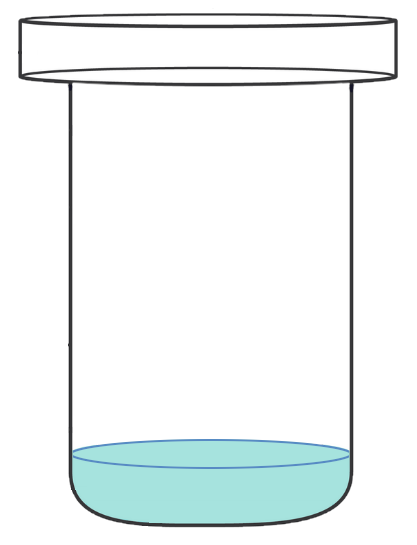
\includegraphics[height=0.15\textheight]{images/chimie/CCM/CCM_etapes_cuve.png}
      
      Remplir jusqu'à environ \qty{0,5}{\cm} de hauteur d'éluant la cuve à CCM.
    \end{center} 
    
    \begin{center}
      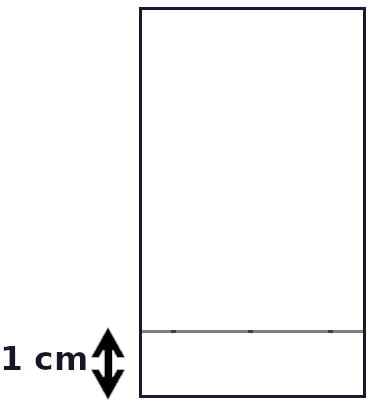
\includegraphics[height=0.15\textheight]{images/chimie/CCM/CCM_etapes_trait.png}
      
      Tracer au crayon à papier un trait à \qty{1}{\cm} du bord inférieur.
    \end{center}
  
    \begin{center}
      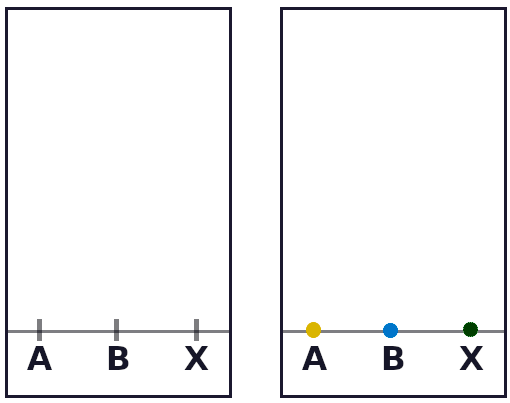
\includegraphics[height=0.15\textheight]{images/chimie/CCM/CCM_etapes_depot.png}
      Marquer des emplacements,
      puis prélever chaque échantillon avec un cure dent et les déposer sur un des emplacements.
    \end{center}
  \end{multicols}
  
  \bigskip
  
  \begin{multicols}{2}
    \begin{center}
      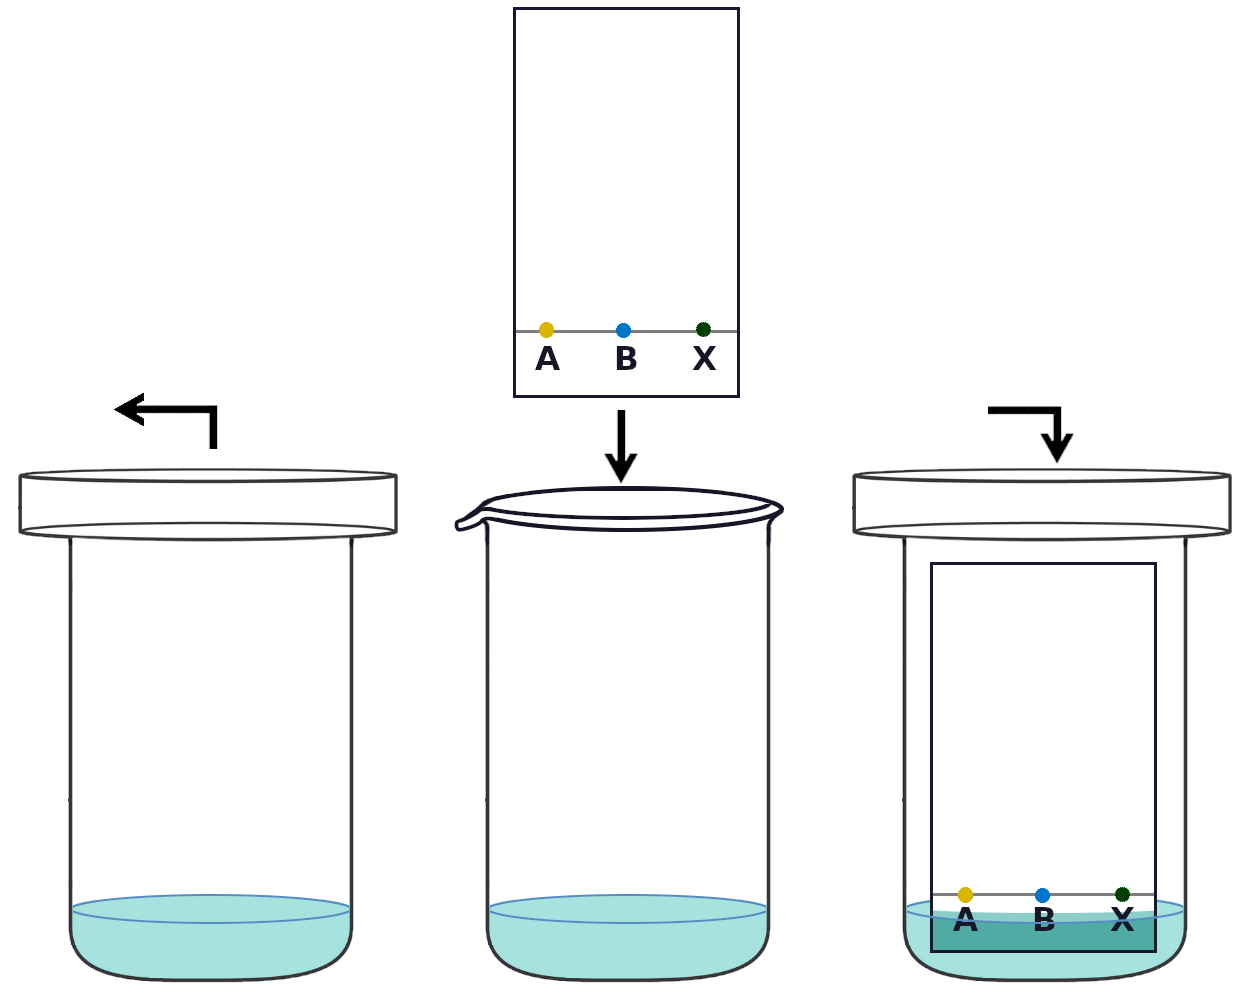
\includegraphics[height=0.25\textheight]{images/chimie/CCM/CCM_etapes_ajout.png}
      
      Poser doucement la plaque dans la cuve en la tenant par les côtés et fermer la cuve.
      \textbf{Ne jamais déplacer la cuve} et attendre que l'éluant monte.
    \end{center}

    \begin{center}
      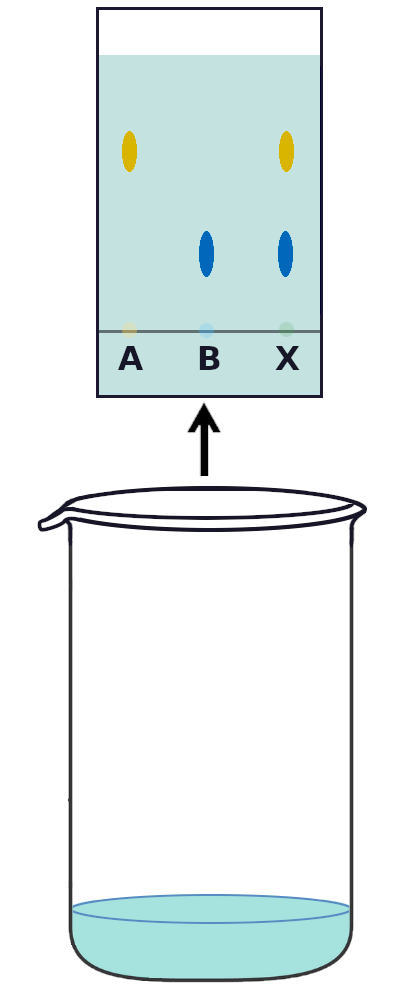
\includegraphics[height=0.25\textheight]{images/chimie/CCM/CCM_etapes_retrait}
      
      Quand le front de l'éluant s'approche du haut, sortir la plaque.
      Tracer une ligne indiquant la hauteur où l'éluant est monté.
    \end{center}
  \end{multicols}
\end{doc}


%%%% questions
\mesure
Placer un M\&M's dans chaque tube à essais et les recouvrir d'eau.
Attendre que le colorant se soit dissous dans l'eau et récupérer les M\&M's.

\mesure
Réaliser le protocole du document~\ref{doc:TP4_protocole_CCM}, avec un dépôt de colorant jaune, un dépôt de colorant bleu et deux dépôts des solutions préparées précédemment.

\mesure
Coller ici le chromatogramme \textbf{sec} et entourer les différentes tâches au crayon à papier.
\pasCorrection{\vspace*{240pt}}

\question{
  Pourquoi doit-on placer la ligne de dépôt au dessus du niveau de l'éluant ?
}{
  Si on la place en dessous, le dépôt va se diluer dans l'éluant et ne montera pas sur la plaque.
}{2}

\question{
  Pourquoi ne doit-on pas déplacer la cuve pendant la montée de l'éluant ?
}{
  Si on déplace la cuve, l'éluant va monter de manière irrégulière, ce qui va fausser l'analyse des résultats.
}{2}


%%%%
\begin{doc}{Lecture d'un chromatogramme}{doc:TP4_lecture_chromato}
  \begin{multicols}{2}
    \begin{listePoints}
      \item \textbf{Lecture verticale :} si le dépôt d'un échantillon se sépare en plusieurs tâches, il s'agit d'un mélange.
      \item \textbf{Lecture horizontale :} sur une même plaque, une même espèce chimique migre toujours à la même hauteur.
    \end{listePoints}
    \vfill \strut

    \centering
    \image{0.7}{images/chimie/CCM/chromatogramme_TP.png} \\
    \footnotesize{schéma d'un chromatogramme}
  \end{multicols}
\end{doc}

%%%%
\begin{doc}{Colorants alimentaires}{doc:TP4_colorants_alimentaire}
  \begin{listePoints}
    \item \textbf{E102 : jaune de tartrazine.} Son usage doit s'accompagner en France de la mention \og peut avoir des effets indésirables sur l'activité et l'attention chez les enfants \fg.
    \item \textbf{E133 : bleu brillant.} Un enfant de 40 kg peut ingérer jusqu'à $240\unit{mg}$ de bleu brillant en une journée. Au-delà le conseil européen indique que ce produit peut être toxique.
  \end{listePoints}
\end{doc}

\question{
  En analysant le chromatogramme à l'aide du document~\ref{doc:TP4_lecture_chromato}, indiquer si les échantillons sont des corps purs ou des mélanges.
}{
  Pour le bleu et le jaune, on a des corps purs (une seule tâche).
  Pour le vert on a un mélange, car le dépôt s'est séparé en deux tâches.
}{4}

\question{
  En utilisant le chromatogramme, donner la composition des colorants présents sur la couche externe des M\&M's.
}{
  Le jaune et le bleu du M\&M's montent à la même hauteurs que les dépots de colorant jaune E102 et bleu E133, ce sont donc les mêmes espèces chimiques.
}{6}


\pasCorrection{\newpage}
%%%% Contexte
\begin{contexte}
  Les huiles essentielles sont obtenues à partir de végétaux pressés ou par distillation fractionnée.
  Les huiles essentielles sont riches en molécules odorantes.
  
  \problematique{
    Comment décrire la composition d'une huile essentielle à l'aide d'une CCM ?
  }
\end{contexte}


%%%% docs
\separationBlocs{
  %%
  \begin{doc}{Huile essentielle de citron et d'orange}{doc:TP4_huile_essentielle}
    L'huile essentielle d'orange (HEO) et l'huile essentielle de citron (HEC)
    sont obtenues en pressant les zestes d'une orange et d'un citron respectivement.
  \end{doc}
}[0.31]{
  %%
  \begin{doc}{Odorat et molécules odorantes}{doc:TP4_molecules_odorantes}
    Chez les humains, Les molécules odorantes sont captées par des neurones de l’épithélium olfactif,
    puis ces neurones transmettent l'information nerveuse au cerveau qui y associe une odeur.
  
    Voilà quelques exemples de molécules odorantes :
    \begin{listePoints}
      \item le \important{limonène} (LIM), est associé à une odeur d'orange.
      \item le \important{linalol} (LIN), est associé à une odeur fraiche et florale.
      \item le \important{géraniol} (G), est associé à une odeur de rose.
      \item le \important{citral} (C), est associé à une odeur de citron.
    \end{listePoints}
  \end{doc}
}[0.69]


%%%%
\question{
  Quelles molécules odorantes peut-on trouver dans l'huile essentiel de citron et d'orange ?
}{
  D'après les descriptions du document~\ref{doc:TP4_molecules_odorantes},
  on s'attend à trouver du limonène dans l'huile essentielle d'orange et du citral dans l'huile essentielle de citron.
}{2}

\begin{doc}{Résultat d'une CCM}{doc:TP4_HEC_HEO}
  On a réalisé deux CCM pour déterminer la composition des huiles essentielles d'orange et de citron.
  \begin{center}
    \image{0.25}{images/donnees/chromato_HEC}
    \image{0.25}{images/donnees/chromato_HEO}
  \end{center}
\end{doc}

\question{
  En analysant les chromatogrammes, donner la composition de l'HEC et l'HEO.
}{
  On trouve du limonène, du géraniol et du citral dans l'HEC (tâches à la même hauteur).
  On trouve du limonène et du géraniol dans l'HEO.
}{5}

  % %%%%
\teteSndCorp

%%%% titre
%\vspace*{-36pt}
\numeroActivite{2}
\titreActivite{Mesure de la masse volumique de l'air}


%%%% objectifs
\begin{objectifs}
  \item Calculer la masse volumique de l'air.
\end{objectifs}

\begin{contexte}
  L'atmosphère est un mélange de plusieurs gaz : dioxygène, diazote, dioxyde de carbone, etc.
  
  \problematique{
    Comment calculer la masse volumique de l'air à partir de sa composition ou d'une expérience ?
  }
\end{contexte}


%%%% docs
\begin{doc}{Mesure de la masse volumique de l'air}{doc:A2_mesure_densite_air}
  \begin{wrapfigure}{r}{0.1\linewidth}
    \vspace*{-29pt}
    \qrcode{https://www.youtube.com/watch?v=isEo51ncsKU&t=26s}
  \end{wrapfigure}
  On peut mesurer la masse volumique de l'air en dégonflant un ballon dans une bouteille d'eau.
  La bouteille d'eau permet de mesurer le volume d'air expulsé.
  En pesant le ballon avant et après le dégonflage, on peut calculer la masse d'air expulsée.
\end{doc}

\numeroQuestion 
Schématiser les 3 étapes de l'expérience réalisée.
\pasCorrection{\vspace*{200pt}}
\correction{
  Schéma du ballon sur la balance avec $m_1$,
  schéma du ballon vidé dans une éprouvette graduée avec l'air qui prend la place de l'eau,
  schéma du ballon sur la balance avec $m_2$.
}

\numeroQuestion
Remplir le tableau ci-dessous 
\begin{tableau}{|c |c |c |c |}
  Grandeur & Masse du ballon plein $m_1 $ & Masse du ballon dégonflé $m_2$ & Volume d'air expulsé $V$ \\
  \SetCell{couleurPrim!10} Valeur & \correction{\qty{483,2}{\g}} & \correction{\qty{481,4}{\g}} & \correction{\qty{1,5}{\litre}}
\end{tableau}

\question{
  Calculer la masse volumique mesurée $\rho_\text{mes}(\text{air})$.
}{
  La masse d'air expulsée est $m = m_2 - m_1 = \qty{1,8}{\g}$, soit une masse volumique
  \begin{equation*}
    \rho = \dfrac{m}{V} = \frac{1,8}{1,5} \unit{\g\per\litre} = \qty{1,2}{\g\per\litre}
  \end{equation*}
}{3}

%%
\begin{doc}{Masse volumique d'un mélange}{doc:A2_composition_atmo}
  Pour un mélange de gaz, la masse volumique du mélange est simplement la somme des masses volumique de chaque gaz pondérée par la fraction volumique de chaque gaz du mélange.

  Pour l'air, on aura donc
  \begin{equation*}
    \rho(\text{air}) = p_v(\chemfig{O_2}) \rho(\chemfig{O_2}) + p_v(\chemfig{N_2}) \rho(\chemfig{N_2}) + p_v(\chemfig{Ar}) \rho(\chemfig{Ar}) + p_v(\chemfig{CO_2}) \rho(\chemfig{CO_2})
  \end{equation*}
\end{doc}

\pasCorrection{\newpage}
\question{
  Rappeler les fractions volumique des gaz composant l'air (\chemfig{O_2}, \chemfig{N_2}, \chemfig{CO_2}, \chemfig{Ar}).
}{
  $p_v(\chemfig{O_2})  = \qty{21}{\percent}$, 
  $p_v(\chemfig{N_2})  = \qty{78}{\percent}$, 
  $p_v(\chemfig{CO_2}) = \qty{0,04}{\percent}$, 
  $p_v(\chemfig{Ar})   = \qty{0,9 }{\percent}$, 
}{2}

\begin{doc}{Masse volumique des gaz composant l'air}{doc:A2_masse_volumique_gaz}
  \textbf{Données :}
  \begin{listeTirets}
    \item Masse volumique du \chemfig{CO_2} gazeux : $\rho(\chemfig{CO_2}) = \qty{1,87}{\g/\litre}$.
    \item Masse volumique du \chemfig{O_2}  gazeux : $\rho(\chemfig{O_2})  = \qty{1,35}{\g/\litre}$.
    \item Masse volumique du \chemfig{N_2}  gazeux : $\rho(\chemfig{N_2})  = \qty{1,18}{\g/\litre}$.
    \item Masse volumique de \chemfig{Ar}   gazeux : $\rho(\chemfig{Ar})   = \qty{1,78}{\g/\litre}$.
  \end{listeTirets}
\end{doc}


%%%%
\question{
  Calculer la masse volumique théorique de l'air $\rho_\text{theo} (\text{air})$.
}{
  $\rho_\text{theo} (\text{air}) 
  = (0,21\times 1,35 + 0,78\times 1,18 + 0,0004\times 1.87 + 0.009\times 1.78) \unit{\g/\litre}
  = \qty{1.22}{\g/\litre}$
}{4}

\question{
  Comparer la valeur théorique et la valeur mesurée. Est-ce qu'elles sont égales ? Est-ce qu'elles sont cohérentes ?
}{
  On trouve deux valeurs légèrement différentes, \qty{1,2}{\g/\litre} et \qty{1,22}{\g/\litre}, mais elles sont cohérentes avec la précision des mesures réalisées pendant l'expérience.
}{2}

  %% Solutions
  % %%%% début de la page
\teteSndSolu

%%%% titre
\vspace*{-36pt}
\numeroActivite{1}
\titreTP{Dosage du sucre par étalonnage}

%%%% objectifs
\begin{objectifs}
  \item Apprendre le vocabulaire sur les solutions.
  \item Comprendre la notion de concentration massique
  \item Comprendre le principe de la dilution et de la dissolution
\end{objectifs}


%%%% contexte
\begin{contexte}
  Le sucre couramment présent dans notre alimentation est le saccharose.
  Cette espèce chimique peut entraîner des risques pour la santé si on en consomme trop.
  Il est donc important de pouvoir déterminer la quantité de sucre consommée par jour.

  \problematique{Comment déterminer la masse de saccharose présent dans un sirop ?}
\end{contexte}


%%%% documents
\begin{doc}{Solution, solvant et soluté}{doc:TP1_solution}
  \begin{importants}
    \chevron Une \important{solution} est un mélange homogène. \\
    Le \important{solvant} est le composant majoritaire du mélange.
    Les \important{solutés} sont les espèces qui sont dispersées dans le solvant.
  \end{importants}
  
  \begin{center}
    \important{Solvant + Soluté(s) = Solution}
  \end{center}
  
  \begin{importants}
    On parle de \important{solution aqueuse} si le solvant est l'eau \chemfig{H_2 O}.
  \end{importants}
\end{doc}

\begin{doc}{Composition d'un sirop}{doc:TP1_sirop}
  Le constructeur annonce que le sirop est composé d'\textit{eau}, de \textit{sucre} de \textit{jus de citron} et d'\textit{acide citrique} principalement.
\end{doc}


\question{
  Donner le solvant et les solutés présents dans le sirop.
}{
  Le solvant du sirop est l'eau, les solutés sont le sucre, le jus de citron et l'acide citriques.
}{2}


%%%%
\begin{doc}{Concentration en soluté}{doc:TP1_concentration}
  \begin{importants}
    La \important{concentration massique $\mathbf{c}$} mesure la quantité de soluté présent dans une solution.
    C'est le rapport de la masse $m$ de \textbf{soluté} dissous dans le volume $V$ de la \textbf{solution}
    \begin{equation*}
      c = \frac{m_\text{soluté}}{V_\text{solution}}
    \end{equation*} 
  \end{importants}
  % \attention Il faut bien distinguer \textbf{concentration massique} et \textbf{masse volumique}.
  % La concentration mesure la masse de soluté contenue dans une solution.
  % La masse volumique mesure la masse d'un échantillon contenue dans un volume donné.
\end{doc}


\begin{doc}{Dissolution du sucre dans l'eau}{doc:TP1_protocole_dissolution}
  \begin{protocole}
      \item Peser une masse donnée de sucre avec une balance de précision.
      \item Mettre le sucre dans une fiole jaugée de 50 mL.
      \item Compléter la fiole jaugée jusqu'à mi-hauteur avec de l'eau distillée, agiter.
      \item Compléter jusqu'au trait de jauge avec de l'eau distillée.
      \item Verser le mélange dans un bêcher de 100 mL.
  \end{protocole}
\end{doc}


%%%% questions
\newpage
\vspace*{-28pt}

\mesure
En utilisant le Document~\ref{doc:TP1_protocole_dissolution}, préparer un mélange de \qty{50}{\ml} d'eau et de de sucre.

\mesure
Mesurer et noter la masse volumique du mélange préparé $\rho =$ \texteTrou[0.1]{\qty{0,15}{\g/\ml}}

\question{
  Calculer la concentration massique de sucre dans la solution aqueuse préparé.
}{
  Avec une masse de sucre de $\qty{10}{\g}$, on a une concentration massique 
  \begin{equation*}
    c = \dfrac{\qty{10}{\g}} {\qty{50}{\ml}}
    = \qty{0,2}{\g/\ml}
  \end{equation*}
}{1}


%%%%
\begin{doc}{Mesure de concentration}{doc:TP1_dosage}
  \begin{importants}
    On parle de \important{dosage} quand on mesure la concentration d'une espèce chimique présente dans une solution.
  \end{importants}
  \begin{importants}
    Un \important{dosage par étalonnage} consiste à déterminer la concentration d’une espèce chimique en comparant une grandeur physique caractéristique de la solution, à la même grandeur physique mesurée pour des solutions étalon.
  \end{importants}
\end{doc}
 
\numeroQuestion 
En utilisant le papier millimétré, tracer la masse volumique en fonction de la concentration massique de sucre dans l'eau.

\numeroQuestion
En déduire la concentration massique de sucre dans la sirop $c_\text{sirop} =$ \texteTrou[0.1]{\qty{0,6}{\g/\ml}}


%%%%
\begin{doc}{Principe d'une dilution}{doc:TP1_principe_dilution}
  \begin{wrapfigure}[5]{r}{0.5\linewidth}
    \vspace*{-16pt}
    \centering
    \begin{multicols}{4}
    \image{1.1}{images/chimie/protocoles/dissoDilu0007} \\[0pt]
    \footnotesize{$S_0$}
    
    \image{1.1}{images/chimie/protocoles/dissoDilu0008}
    
    \image{1.1}{images/chimie/protocoles/dissoDilu0010}
    
    \image{1.1}{images/chimie/protocoles/dissoDilu0011} \\[0pt]
    \footnotesize{$S_1$}
    \end{multicols}
  \end{wrapfigure}
  \vAligne{-40pt}
  
  \begin{importants}
    Le principe de la \important{dilution} est de \important{diminuer la concentration} en soluté dans une solution en rajoutant du \important{solvant.}
  \end{importants}
  La solution de départ est appelée \important{solution mère}, notée $S_0$.
  La solution obtenue après dilution est appelée \important{solution fille}, notée $S_1$.

  Pour diluer une solution, il faut
  \begin{protocole}
    \item Prélever un volume $V_0$ de la solution à l'aide de la pipette graduée.
    Le bas du ménisque doit atteindre la graduation supérieure.
    \item Introduire la solution prélevée dans la fiole jaugée de volume $V_1$.
    \item Ajouter de l'eau distillée dans la fiole jaugée jusqu'aux $2/3$ et agiter doucement. Compléter jusqu'à ce que le bas du ménisque atteigne le trait de jauge.
    \item Fermer la fiole et l'agiter en la retournant plusieurs fois.
    \item Verser la solution fille obtenue dans un bécher.
  \end{protocole}
\end{doc}


%%%%
\begin{doc}{Facteur de dilution}{doc:TP1_dilution}  
  Le \important{facteur de dilution} est le rapport du volume de la solution fille sur le volume de la solution mère
  \begin{equation*}
    F = \frac{V_\text{1}}{V_\text{0}}
  \end{equation*}
  On dit qu'on a dilué $F$ fois une solution.
\end{doc}

\mesure 
Diluer \textbf{2 fois} le sirop et mesurer sa masse volumique. 

\question{
  En déduire la concentration massique en sucre.
  Que constatez-vous ?
}{
  Pour diluer 2 fois, il faut que $F = 2 = \dfrac{V_\text{1}}{V_\text{0}}$, on aura donc un volume final $V_\text{1} = 2\times V_\text{0}$ deux fois plus grand que le volume initial, avec donc une concentration massique 2 fois plus faible.

  On constate que la concentration massique a été divisée par le facteur de dilution.
}{0}

  % %%%% début de la page
\teteSndSolu

%%%% titre
\vspace*{-36pt}
\numeroActivite{1}
\titreActivite{Mal de tête et dissolution}

%%%% objectifs
\begin{objectifs}
  \item Calculer une concentration massique.
\end{objectifs}


%%%% contexte
\begin{contexte}
  Inès, 8 ans, a mal à la tête et son père décide de lui donner du paracétamol pour la soulager, sauf qu'il ne possède que des comprimés pour adulte !

  \problematique{Comment le père va-t-il calculer la bonne dose à administrer à sa fille ?}
\end{contexte}


%%%% documents
\begin{doc}{Solution, solvant et soluté}{doc:A1_solution}
  \begin{importants}
    Une \important{solution} est un mélange homogène.
    Le \important{solvant} est le composant majoritaire du mélange.
    Les \important{solutés} sont les espèces qui sont dispersées par le solvant.
    \begin{center}
        \important{solvant + solutés = solution}
    \end{center}
  \end{importants}
\end{doc}

\begin{doc}{Le paracétamol}{doc:A1_paracétamol}
  \begin{wrapfigure}[5]{r}{0.3\linewidth}
    \vspace*{-30pt}
    \centering
    \chemname{\chemfig{!\paracetamol}}{paracétamol}
  \end{wrapfigure}
  
  Le paracétamol est un antidouleur qui peut être dangereux pour le foie s'il est consommé en trop grande quantité.
  Un comprimé pour adulte a une masse $m_1 = \qty{500}{\milli\g}$, alors qu'un comprimé pour enfant a une masse $m_2 = \qty{300}{\milli\g}$.
  
  Pour calmer le mal de tête d'Inès, le père décide qu'il va \important{dissoudre} un comprimé de paracétamol pour adulte dans un verre d'eau de volume $V_1 = \qty{25}{\centi\litre}$.
\end{doc}


\question{
  Donner le solvant et les solutés de la solution préparée par le père.
}{
  Le solvant de la solution est l'eau, le soluté est le paracétamol.
}{2}


\begin{doc}{Concentration massique}{doc:A1_concentration_massique}
  \begin{importants}
    La \important{concentration massique $\mathbf{c}$} mesure la quantité de soluté présent dans une solution.
    C'est le rapport de la masse de \important{soluté} dissous sur le volume total de la \important{solution}
    \begin{equation*}
      c = \frac{m_\text{soluté}}{V_\text{solution}}
    \end{equation*}
  \end{importants}
\end{doc}

\question{
  Convertir le volume $V_1$ de la solution en millilitre, noté \unit{\ml}.
}{
  \begin{equation*}  
    V_1 = \qty{25}{\centi\litre} = \qty{250}{\ml}
  \end{equation*}
}{1}

\question{
  Calculer la concentration $c$ en \unit{\mg/\ml} de paracétamol dans le verre d'eau.
}{
  \begin{equation*}
    c = \dfrac{m_1}{V_1}
      = \dfrac{\qty{500}{\mg}} {\qty{250}{\ml}}
      = \qty{2,0}{\mg/\ml}
  \end{equation*}
}{4}

\newpage
\question{
  Quel volume $V_2$ de la solution (du verre d'eau) Inès doit-elle boire pour avaler $m_2 = \qty{300}{\milli\g}$ de paracétamol ?
}{
  \begin{equation*}
    V_2 = \dfrac{m_2}{c}
        = \dfrac{\qty{300}{\mg}} {\qty{2,0}{\mg/\ml}}
        = \qty{150}{\ml}
        = \qty{15,0}{\centi\litre}
  \end{equation*}
}{6}

  % %%%% début de la page
\teteSndSolu


%%%% titre
\vspace*{-36pt}
\numeroActivite{2}
\titreTP{Dosage d'un antiseptique}


%%%% objectifs
\begin{objectifs}
  \item Comprendre la notion de concentration massique.
  \item Doser la quantité de permanganate de potassium présente dans du Dakin.
\end{objectifs}


%%%% contexte
\begin{contexte}
  Le Dakin est une solution antiseptique qui sert à nettoyer des plaies. Le principe actif du Dakin est stabilisé par l'ajout de permanganate de potassium \chemfig{KMnO_4}.
  Le permanganate de potassium donne une teinte violette au Dakin.
  
  \problematique{Comment mesurer la concentration en \chemfig{KMnO_4} dans le Dakin ?}
\end{contexte}


%%%%
\begin{doc}{Concentration en soluté}{doc:TP2_concentration}
  \begin{importants}
    La \important{concentration massique $\mathbf{c}$} mesure la quantité de soluté présent dans une solution.
    C'est le rapport de la masse $m$ de \textbf{soluté} dissous dans le volume $V$ de la \textbf{solution}
    \begin{equation*}
      c = \frac{m_\text{soluté}}{V_\text{solution}}
    \end{equation*}
  \end{importants}
\end{doc}


%%%%
\begin{doc}{Dakin}{doc:TP2_dakin}
  Le Dakin est une solution aqueuse d'hypochlorite de sodium \chemfig{Na ClO}.
  Du permanganate de potassium \chemfig{K MnO_4} est ajouté à la solution, pour qu'elle ne soit pas dégradée par l'exposition au rayonnement UV du Soleil.
  
  \fleche Sur une bouteille de Dakin il est indiqué que la concentration de \chemfig{KMnO_4} vaut $\approx \qty{0,01}{\g/\litre}$.
\end{doc}

%
\question{
  Donner le solvant et les solutés de la solution de Dakin.
}{
  Le solvant est l'eau, les solutés sont le permanganate de potassium et l'hypochlorite de sodium.
}{2}


%%%%
\begin{doc}{Mesure de concentration d'une solution colorée}{doc:TP2_dosage}  
  \begin{importants}
    Une \important{échelle de teinte} permet de mesurer la concentration d'un soluté coloré.
  \end{importants}

  La teinte d'une solution est proportionnelle à la concentration en soluté.
  On prépare une série de solutions \textbf{étalons} dont on connaît la concentration et on compare leur teinte avec la solution dont on veut mesurer la concentration.
  
  \attention Il faut comparer les teintes avec des verreries identiques, la teinte s'assombrit avec l'épaisseur.
\end{doc}


%%%%
\begin{doc}{Protocole d'une dilution}{doc:TP2_protocole_dilution}
  \begin{wrapfigure}[5]{r}{0.5\linewidth}
    \vspace*{-20pt}
    \centering
    \begin{multicols}{4}
    \image{1.1}{images/chimie/protocoles/dissoDilu0007} \\[0pt]
    \footnotesize{$S_0$}
    
    \image{1.1}{images/chimie/protocoles/dissoDilu0008}
    
    \image{1.1}{images/chimie/protocoles/dissoDilu0010}
    
    \image{1.1}{images/chimie/protocoles/dissoDilu0011} \\[0pt]
    \footnotesize{$S_1$}
    \end{multicols}
  \end{wrapfigure}
  \vAligne{-40pt}
  
  \begin{importants}
    La \important{dilution} est la \important{diminution de la concentration} en soluté d'une solution en rajoutant du \important{solvant.}
  \end{importants}
  La solution de départ est appelée \important{solution mère}, notée $S_0$.
  La solution obtenue après dilution est appelée \important{solution fille}, notée $S_1$.

  Pour diluer une solution, il faut
  \begin{protocole}
    \item Prélever un volume $V_0$ de la solution à l'aide d'une pipette graduée.
    \textbf{Le bas du ménisque} doit atteindre la graduation supérieure.
    \item Introduire la solution prélevée dans la fiole jaugée de volume $V_1$.
    \item Ajouter de l'eau distillée dans la fiole jaugée jusqu'aux $2/3$ et agiter doucement.
    Compléter jusqu'à ce que \textbf{le bas du ménisque} atteigne le trait de jauge.
    \item Fermer la fiole et l'agiter en la retournant plusieurs fois.
    \item Verser la solution fille obtenue dans un bécher.
  \end{protocole}
\end{doc}

%%%%
\begin{doc}{Facteur de dilution}{doc:TP1_dilution}  
  Le \important{facteur de dilution} est le rapport du volume de la solution fille sur le volume de la solution mère et il est égal au rapport des concentrations des solutions mère et fille.
  \begin{equation*}
    F = \dfrac{V_1}{V_0} = \dfrac{c_0}{c_1}
  \end{equation*}
\end{doc}


%
\question{
  On souhaite réaliser une échelle de teinte composée de 4 solutions étalon pour mesurer la concentration de permanganate de potassium dans le Dakin.

  \begin{center}
    \begin{tblr}{c | X[1,c] | X[1,c] | X[1,c] | X[1,c]}
      Solution étalon & 1 & 2 & 3 & 4 \\ \hline
      Concentration (\unit{\g/\litre}) & \correction{\num{0,05}} & \correction{\num{0,025}} & \correction{\num{0,0125}} & \correction{\num{0,0063}} 
    \end{tblr}
  \end{center}
  
  Calculer le facteur de dilution entre les différentes solutions.
}{
  On divise par deux la concentration pour passer de la solution 1 à la solution 2, de la 2 à la 3 et de la solution 3 à la solution 4.
  Donc le facteur de dilution est $F = 2$.
}{1}

%
\question{
  Justifier l’intervalle des concentrations proposées pour l’échelle de teinte, à partir de la valeur attendue de la concentration en permanganate de potassium.
}{
  La valeur attendue de la concentration ($c = \qty{0,01}{\g/\litre}$) se trouve bien dans l'intervalle proposé.
}{1}

%
\question{
  Sachant que le volume de la fiole jaugée est $V_1 = \qty{50}{\ml}$, donner le volume de la solution mère $V_0$ à prélever pour avoir un facteur de dilution $F = 2$.
}{
  On doit avoir un volume deux fois plus faible, soit $V_0 = \qty{25}{\ml}$.
}{2}

%
\mesure
Réaliser l'échelle de teinte en effectuant trois dilutions successives.
Verser quelques millilitres de chaque solutions dans des tubes à essais.

%
\mesure
Utiliser l'échelle de teinte pour encadrer la valeur de la concentration en permanganate de potassium dans le Dakin.
Est-elle cohérente avec celle du constructeur ?
\pasCorrection{\lignesDeReponse{2}}
\correction{Oui, on trouve une concentration $\qty{0,0125}{\g/\litre} < c < \qty{0,0063}{\g/\litre}$.}

%
\question{
  Proposer une autre échelle de teinte pour améliorer la précision de la mesure (donner une liste de concentration).
}{
  On pourrait utiliser une échelle de teinte avec les concentrations suivantes : 0.015, 0.012, 0.0094, 0.0075, 0.006 \unit{\g/\litre} ($F = 1.25$).
}{1}

  % %%%% début de la page
\teteSndSolu

%%%% titre
\vspace*{-36pt}
\numeroActivite{2}
\titreActivite{Hémoglobine et anémie}

%%%% objectifs
\begin{objectifs}
  \item Mesurer une concentration massique à l'aide d'une échelle de teinte
\end{objectifs}


%%%% contexte
\begin{contexte}
  Pour assurer son bon fonctionnement, l'organisme d'un être humain a besoin de fer \chemfig{Fe}.
  On dit qu'une personne souffre d'anémie si la concentration massique en fer dans le sang est trop faible.
  Le fer est transporté par une molécule dans le sang : l'hémoglobine.

  \problematique{Comment vérifier qu'une personne ne souffre pas d'anémie ?}
\end{contexte}


%%%% documents
\begin{doc}{Concentration en hémoglobine}{doc:A2_anemie}
  Mesurer la concentration massique en hémoglobine dans le sang permet de détecter les cas d'anémies.
  On parle d'anémie si cette concentration massiques est inférieure a
  \qty{1,2}{\g\per\litre} pour une femme et \qty{1,3}{\g\per\litre} pour un homme.
  Pour mesurer cette concentration, on peut réaliser une échelle de teinte, car c'est l'hémoglobine qui donne sa teinte rouge au sang.

  \separationBlocs{
    \begin{center}
      \begin{tblr}{c | c | c | c | c | c}
        Solution &
        {\tubeEssaisSolution{rougeClair}          \\ 1} &
        {\tubeEssaisSolution{rougeClair!70!white} \\ 2} &
        {\tubeEssaisSolution{rougeClair!40!white} \\ 3} &
        {\tubeEssaisSolution{rougeClair!15!white} \\ 4} &
        {\tubeEssaisSolution{rougeClair!5!white}  \\ 5} \\ \hline
        %
        Concentration \unit{\g\per\litre} & 1,4 & 1,3 & 1,2 & 1,1 & 1,0 \\ \hline
      \end{tblr} \\[4pt]
      
      Schéma de l'échelle de teinte réalisée, avec les solutions étalons et leurs concentrations.
    \end{center}
  }[0.6]{
    \begin{center}
      \tubeEssaisSolution{rougeClair!55!white}
  
      Échantillon de sang à doser.
    \end{center}
  }[0.4]
\end{doc}

%
\question{
  Rappeler avec vos mots le principe général d'un dosage par étalonnage (que veut-on mesurer et comment fait-on).
}{
  On cherche à mesurer une concentration en comparant les teintes de différentes solutions.
  C'est possible, car la teinte est proportionnelle à la concentration.
}{3}

%
\question{
  Pour préparer des solutions, on peut effectuer une dilution ou une dissolution. Indiquer en justifiant laquelle des deux méthode on utilise pour passer de la solution 2 à la solution 3.
}{
  On réalise une dilution, car on diminue la concentration.
}{2}

%
\question{
  En utilisant la figure du document~\ref{doc:A2_anemie}, indiquer en justifiant la concentration en hémoglobine de l'échantillon de sang.
}{
  La teinte de l'échantillon se trouve entre celle de la solution 2 et 3,
  donc sa concentration se trouve entre 1,3 et \qty{1,2}{\g\per\litre} d'hémoglobine.
}{3}

%
\question{
  L'échantillon vient d'une femme. Indiquer en justifiant si elle souffre d'anémie ou non.
}{
  Elle ne souffre pas d'anémie, car sa concentration en hémoglobine est supérieure à \qty{1,2}{\g\per\litre}.
}{2}

  % 
\begin{tableau}{ c | c }
  Masse volumique (g/mL) & Concentration en sucre (g/mL) \\
  \num{1.00} & \num{0.01} \\
  \num{0.99} & \num{0.01} \\
  \num{1.03} & \num{0.02} \\
  \num{1.03} & \num{0.03} \\
  \num{1.03} & \num{0.04} \\
  \num{1.03} & \num{0.04} \\
  \num{1.03} & \num{0.05} \\
  \num{1.04} & \num{0.06} \\
  \num{1.04} & \num{0.06} \\
  \num{1.05} & \num{0.07} \\
  \num{1.08} & \num{0.08} \\
  \num{1.07} & \num{0.09} \\
  \num{1.08} & \num{0.09} \\
  \num{1.09} & \num{0.11} \\
\end{tableau}
  %% Mecanique
  % %%%% début de la page
\teteSndMouv

%%%%
\nomPrenomClasse


%%%% titre
\numeroActivite{1}
\titreTP{Décrire le mouvement}


%%%% objectifs
\begin{objectifs}
  \item Décrire un mouvement.
  \item Comprendre la notion de référentiel.
  \item Comprendre que le mouvement dépend du référentiel.
\end{objectifs}


%%%% evaluation
\begin{tableauCompetences}
  APP &
  Représenter une situation par un schéma avec une légende.
  & & & & \\
  %
  COM &
  Travailler en groupe, communiquer à l'oral.
  & & & & \\
\end{tableauCompetences}

%%%%
\vspace*{6pt}
\begin{doc}{Un peu de vocabulaire}{doc:TP1_vocabulaire}
  \begin{importants}
    \important{Système} : objet dont on étudie le mouvement.
  \end{importants}
  
  \begin{importants}
    \important{Trajectoire} : ensemble des positions successives occupées par le système.
  \end{importants}
  
  Le \important{mouvement} d'un système est donné par la description de sa trajectoire et de l'évolution de sa vitesse.
\end{doc} 


\begin{doc}{Type de trajectoires}{doc:TP1_trajectoires}
  Trajectoire \important{rectiligne} : \texteTrou{trajectoire représentée par une droite.}
  
  \texteTrou[0.5]{Trajectoire circulaire} : trajectoire représentée par un cercle.
  
  Trajectoire \important{curviligne} : \texteTrou{trajectoire représentée par une courbe.}
\end{doc}


\begin{doc}{Vitesse et accéleration}{doc:TP1_vitesse}
  Vitesse \important{uniforme} (constante) : le système n’accélère pas.
  
  La vitesse augmente : \texteTrouLignes{le système accélère.}
  
  La vitesse diminue : \texteTrouLignes{le système décélère.}
  
  Si \texteTrou[0.5]{la vitesse est constante et nulle}, on dit que le système est \important{immobile}.
\end{doc}


%%%%

\numeroQuestion
Compléter les documents~\ref{doc:TP1_trajectoires} et~\ref{doc:TP1_vitesse}.

\fleche Pour la suite de cette activité, vous allez choisir entre l'étude du mouvement des oies ou de la Lune.
Vous présenterez ensuite les résultats de votre étude au reste de la classe à l'oral.

\fleche Vous rendrez ensuite une compte-rendu détaillée en suivant les questions sur le \important{mouvement que vous n'avez pas choisi.}
Il faudra donc être attentif à ce que disent vos camarades !


%%%%
\newpage
\titreSousSection{\'Etude du mouvement des oies}

Le compteur du bateau affiche une vitesse $v_\text{bateau} = \qty{3,6e1}{\km/\hour}$.

\vspace*{6pt}
\numeroQuestion Pour la personne qui filme les oies, quelle est la vitesse des oies ?

\numeroQuestion Pour une personne se trouvant sur la berge, quelle est la vitesse des oies ?

\numeroQuestion Schématiser la trajectoire des oies si on les observe depuis la berge.

\numeroQuestion Indiquer le mouvement des oies depuis le bateau et la berge.

%%
\titreSousSection{\'Etude du mouvement de la Lune}

La Lune tourne autour de la Terre à une vitesse $v_\text{Lune} = \qty{3,7e3}{\km/\hour}$
et la Terre tourne autour du Soleil à une vitesse $v_\text{Terre} = \qty{1,1e5}{\km/\hour}$.

\begin{figure}[!ht]
  \begin{subfigure}{0.48\linewidth}
    \centering
    \image{0.8}{images/mecanique/terre_lune.png}
    \caption{Point de vue centré sur la Terre}
    \label{fig:terre_lune}
  \end{subfigure}
  \begin{subfigure}{0.48\linewidth}
    \centering
    \image{0.8}{images/mecanique/terre_lune_soleil.png}
    \caption{Point de vue centré sur le Soleil}
    \label{fig:terre_lune_soleil}
  \end{subfigure}
\end{figure}

\vspace*{-6pt}
\numeroQuestion Depuis le point de vue centré sur la Terre, quelle est la vitesse de la Lune ?

\numeroQuestion Schématiser la trajectoire de la Lune depuis ce point de vue et indiquer son mouvement.

\numeroQuestion Peut-on décrire la vitesse de la Lune depuis le point de vue centré sur le Soleil ?

\numeroQuestion Schématiser la trajectoire de la Lune depuis ce point de vue.


%%%%
\titreSousSection{Notion de référentiel}

\question{
  Convertir la vitesse $v_\text{Lune}$ en \unit{\m/\s}.
  \textit{Rappel :} \qty{1}{\km} = \qty{e3}{\metre}, \qty{1}{\hour} = \qty{3,6e3}{\s}.
}{}{2}

\question{
  Quelle distance la Lune parcours pendant 1 seconde ?
  Comparer avec la longueur de sa trajectoire, qui est de \qty{2,4e6}{\km}.
}{}{1}

\question{
  Peut-on décrire la trajectoire de la Lune en l'observant pendant 1 seconde ?
}{}{2}

\question{
  Conclusion : pourquoi est-il important de définir le référentiel, qui est l’endroit où on se place et le temps passé à observer, avant d'étudier un mouvement ?
}{}{1} % 2h
  % %%%% début de la page
\teteSndMouv

%%%% titre
%\nomPrenomClasse
\numeroActivite{1}
\vspace*{-36pt}
\titreActivite{Modéliser le mouvement}


%%%% objectifs
\vspace{-10pt}
\begin{objectifs}
  \item Modéliser le système étudié par un point matériel.
  \item Comprendre que le mouvement dépend du référentiel choisi.
  \item Comprendre l'utilisation des vecteurs en physique.
\end{objectifs}


%%%% evaluation
% \begin{tableauCompetences}
%   COM & Travailler en groupe, échanger entre élèves.
%   & & & &
% \end{tableauCompetences}


%%%%
\vspace*{-12pt}
\titreSection{Système et référentiel}

%%%%
\vspace{-10pt}
\begin{doc}{Modèle du point matériel}{doc:A1_point_materiel}
  \begin{importants}
    \important{Système} : objet dont on étudie le mouvement.
  
    On ne va s'intéresser qu'au mouvement global du système.
    C'est pourquoi on va modéliser le système par
    \texteTrouLignes[2]{
      Un point de même masse que le système, localisé au centre de masse du système.
      C'est le \important{modèle du point matériel.}
    }
  \end{importants}

  \fleche Le modèle du point matériel revient à ignorer toute information sur la géométrie du système étudié. 
  Les éventuelles rotations et déformations ne sont donc pas prises en compte.
\end{doc}


\begin{tblr}{
    colspec = {X[1.5,c,m] | X[1,c,m] | X[2,c] | X[2,c] },
    row{1} = {couleurPrim!20}
  }
  Système & Centre de masse & Trajectoire & Informations perdues \\ \hline
  %
  {\image{1}{images/mecanique/point_balle_tennis.png} \\ Balle de tennis} &
  Centre de la balle & & \\ \hline
  %
  {\image{1}{images/mecanique/point_roue.jpg} \\ Roue} &
  Centre de la roue & & \\ \hline
  %
  {\image{1}{images/mecanique/point_humain_course.jpg} \\ Modèle d'humain} &
  Nombril & &
\end{tblr}

%%
\newpage
\vspace*{-34pt}
\begin{doc}{Référentiel}{doc:A1_referentiel}
  Pour décrire le mouvement, il faut pouvoir le repérer dans l’espace et dans le temps, pour ça on utilise un référentiel.
  
  \begin{importants}
    \important{Référentiel} : \texteTrouLignes[1]{
      objet de référence, muni d'un repère par rapport auquel on étudie le mouvement du système.
    }
  \end{importants}
  
  \begin{importants}
    La description du mouvement dépend du \important{référentiel} choisi.
    On appelle ça la \important{relativité} du mouvement.
  \end{importants}
\end{doc}


%%%%
\titreSection{Vecteur}

%%
\vspace*{-8pt}
\begin{doc}{Vecteur en physique}{doc:A1_vecteur}
  \begin{importants}
    \important{Vecteur} : objet mathématique représenté par un segment fléché $\longrightarrow$ et noté avec une lettre surmontée d'une flèche $\vv{v}$.
    
    Un vecteur contient quatre information : 
    \begin{multicols}{2}
      \begin{listePoints}
        \item \texteTrou{Une direction.}
        \item \texteTrou{Un sens.}
        \item \texteTrou{Une valeur, ou norme.}
        \item \texteTrou{Une origine.}
      \end{listePoints}
    \end{multicols}
  
    Un vecteur est \important{constant} si
    \texteTrouLignes[1]{sa norme, sa direction et son sens sont constants.}
  \end{importants}
  
  \fleche En physique on va se servir des vecteurs pour représenter différentes grandeurs :
  \texteTrouLignes[1]{vitesse, force, champ électromagnétique, aimantation, accéleration, etc.}
  
  \attention Un vecteur n'est \textbf{jamais} égal à un nombre, qui contient moins d'information.
\end{doc}

\begin{doc}{Opération sur les vecteurs}{doc:A1_operation_vecteur}
  Même si les vecteurs ne sont pas des nombres, on peut effectuer des \important{opérations} avec.
  Cette année on ne réalisera que des opérations graphique.
  \begin{multicols}{3}
    \centering
    \begin{boite}
      \vAligne{50pt}
    \end{boite}
    Addition
    
    \begin{boite}
      \vAligne{50pt}
    \end{boite}
    Multiplication par un nombre

    \begin{boite}
      \vAligne{50pt}
    \end{boite}
    Soustraction
  \end{multicols}

  \begin{importants}
    Le \important{vecteur nul}, noté $\vv{0}$, est le vecteur de valeur nulle.
    On l'obtient en soustrayant un vecteur par lui même $\vv{a} - \vv{a} = \vv{a} + (-1 \times \vv{a}) = \vv{0}$.
  \end{importants}
\end{doc} % 1h
  % \input{seconde/mecanique/mecaTP2_vitesse} % 2h
  % %%%% début de la page
\teteSndMouv


%%%% titre
\vspace*{-32pt}
\numeroActivite{2}
\titreActivite{Modéliser une action par une force}


%%%% objectifs
\begin{objectifs}
  \item Comprendre la notion de force
  \item Connaître des exemples de forces
\end{objectifs}

%%%%
\begin{doc}{Force et action mécanique}{doc:A2_action_force}
  \begin{importants}  
    Un corps exerce une \important{action mécanique} sur un système étudié \texteTrouLignes[1]{s’il est capable d’en modifier le mouvement.}
  \end{importants}
  
  Une action mécanique est modélisée par une \important{force.}

  \begin{importants}
    La force exercée par un corps $A$ sur un corps $B$ est représentée par un vecteur $\vvFAsurB$.
    Ce vecteur possède les caractéristiques suivantes :
    \begin{listePoints}
      \item Une \important{valeur} notée $\FAsurB$, qui s'exprime en newton noté \unit{\newton}.
      \item Une \important{direction} et un \important{sens} qui dépendent de la situation.
      \item Une \important{origine}, appelée \important{point d'application} : le centre du système $B$.
    \end{listePoints}
  \end{importants}
\end{doc}

\mesure
Une personne pousse un carton. 
Représenter la force $\vv{F}_\text{personne/carton}$ qu'exerce la personne sur le carton.

\vspace*{-8pt}
\begin{center}
  \image{0.23}{images/mecanique/personne_carton}
\end{center}


%%
\begin{doc}{Exemples de forces}{doc:A2_exemples_forces}
  On distingue 2 types d'actions :
  \begin{listePoints}
    \item les \important{actions de contact} (contact entre l’objet qui donne la force et l’objet qui la reçoit),
    \item les \important{actions à distance} (pas de contact).
  \end{listePoints}
  
  \begin{tblr}{
    colspec = {|c |c |X[c] |}, hlines,
    row{1} = { couleurPrim!20 },
  }
    Force & Valeur & Direction, sens \\
    %
    poids $\vv{P}$ &
    $P = m \times g$ &
    verticale, vers le bas \\
    %
    réaction du support $\vv{R}$ &
    égale au poids $R = P$ &
    perpendiculaire au support, vers le haut \\
    %
    frottements $\vv{f}$ &
    dépend du cas étudié &
    opposés à la vitesse $\vv{v}$ \\
  \end{tblr}
  \smallskip
  
  \begin{listePoints}
    \item $\vv{P}$ représente l'interaction gravitationnelle de la Terre.
    \item $\vv{R}$ représente l'action exercée par le support sur un objet posé dessus.
    \item $\vv{f}$ représentent l'action d'un milieu (gaz, liquide, support solide).
  \end{listePoints}
  \attention Si un objet est \important{immobile par rapport au milieu,} il n'y a pas de frottements.
\end{doc}

\pasCorrection{\vspace*{-16pt}}
\question{
  Parmi les forces $\vv{P}$, $\vv{R}$ et $\vv{f}$, indiquer celles qui modélisent une action de contact et celles qui modélisent une action à distance.
}{
  La réaction du support et les frottements sont des actions de contact.
  Le poids est une action à distance.
}{3}


%%%%
\begin{center}
  \begin{tblr}{
    colspec = {|X[c,m] |X[c,m] |}, hlines,
    row{1,3} = {couleurPrim!20},
  }
    Ballon & Curling \\
    \image{0.8}{images/mecanique/ballon_football} &
    \image{0.8}{images/mecanique/curling} \\
    %
    Parachutiste & Skieuse \\
    \image{0.8}{images/mecanique/parachutiste} &
    \image{0.8}{images/mecanique/skieur} \\  
  \end{tblr}
\end{center}

%%
\mesure 
En vous aidant des documents~\ref{doc:A2_action_force} et~\ref{doc:A2_exemples_forces}, compléter le tableau :
\begin{listePoints}
  \item Schématiser la ou les forces entrant en jeu, en faisant attention à leurs points d'application.
  \item Tracer la somme de toutes les forces entrant en jeu.
\end{listePoints} % 2h
  % %%%% début de la page
\teteSndMouv


%%%% titre
\vspace*{-32pt}
\numeroActivite{3}
\titreActivite{Le principe d'inertie}


%%%% objectifs
\begin{objectifs}
  \item Comprendre la notion d'inertie
  \item Comprendre le principe d'inertie.
\end{objectifs}


\begin{doc}{Inertie d'un corps}{doc:A3_inertie}
  \begin{importants}
    \important{L'inertie} est la tendance qu'ont les corps à rester dans le même état (repos ou mouvement), en l'absence de forces appliquées.
  \end{importants}
    
  \fleche C'est la masse qui le mesure : plus un objet a une masse élevée et plus il a de l'inertie.
  
  \fleche Dis autrement : plus un objet est lourd, plus il faut exercer une force importante pour changer son mouvement.
  
  \exemple Faire rouler un caddie vide est facile, mais c'est plus difficile quand il est rempli !
\end{doc}


\begin{doc}{Forces qui se compensent}{doc:A3_forces_compensent}
  \begin{importants} 
    On dit que des forces se compensent si leur somme est égale au vecteur nul $\vv{0}$.
  \end{importants}
  Pour que la somme de deux vecteurs soit nulles, il faut qu'ils aient même \important{direction,} même \important{valeur,} mais un \important{sens opposé.}
  Pour la somme de trois vecteurs, on commence par sommer deux vecteurs, puis on somme le vecteur obtenu avec le troisième restant.
  
  \centering
  \image{0.72}{images/mecanique/forces_systemes}
\end{doc}

\question{
  Pour quels systèmes du document~\ref{doc:A3_forces_compensent} les forces se compensent-elles ?
}{
  Dans les quatres situations on a des forces qui se compensent, avec une somme des vecteurs nulle. 
}{2}

\question{
  Quel est le mouvement du système dans chaque cas où les forces se compensent ?
}{
  Soit le système est immobile, soit sa vitesse est rectiligne uniforme.

  Dit autrement, pour faire bouger un objet ou pour modifier sa trajectoire, il faut qu'il soit soumis à des forces.
}{2}



\begin{doc}{Le principe d'inertie et sa contraposée}{doc:A3_principe_inertie}
  \chevron Le \important{principe d'inertie} a été formulé pour la première fois par Newton en 1687.
  Newton s'appuyait sur les travaux de Descartes et de Galilée, et parfois on appelle ce principe la \important{première loi de Newton}.
  Sa formulation moderne est la suivante :
  
  \begin{importants}
    Si les forces qui s'exercent sur un système se compensent, alors ce système est \texteTrouLignes[2]{soit immobile, soit en mouvement rectiligne uniforme.}
  \end{importants}
  
  \begin{importants}
    Réciproquement, si un système est
    \texteTrouLignes[3]{immobile ou en mouvement rectiligne uniforme, alors les forces qui s'exercent sur lui se compensent.}
  \end{importants}
\end{doc}


%%%%
\question{
  Comment varie $\vv{v}$ pour un système qui a un mouvement rectiligne uniforme ?
  En déduire la variation de $\vv{v}$ pour un système soumis à des forces qui se compensent.
}{
  Le vecteur vitesse est constant pour un mouvement rectiligne uniforme.
  Donc le vecteur vitesse est constant si le système est soumis à des forces qui se compensent.
}{3}

\begin{doc}{Principe d'inertie et vitesse}{doc:A3_principe_inertie_vitesse}
  \begin{importants}
    Le principe d'inertie dit que si le vecteur vitesse
    \texteTrouLignes[2]{
      est constant sur toute la trajectoire, alors les forces exercées sur le système se compensent.
    }
  \end{importants}
\end{doc} % 1h
  % %%%% début de la page
\teteSndMouv

%%
\nomPrenomClasse


%%%% titre
\numeroActivite{4}
\titreActivite{Principe des actions réciproques}


%%%% evaluation
\vspace*{-8pt}
\begin{tableauCompetences}
  %
  \centering ANA/RAI &
  Analyser les forces qui s'exercent sur un système.
  & & & & \\
  %
  \centering REA &
  Schématiser une situation.
  & & & & \\
  %
  \centering COM &
  Travailler en groupe.
  & & & &
\end{tableauCompetences}


%%%% objectifs
\begin{objectifs}
  \item Analyser et schématiser un système en mouvement
  \item Utiliser le principe d'inertie
  \item Comprendre le principe des actions réciproques
\end{objectifs}


%%%%
\begin{doc}{Forces qui se compensent}{doc:A4_forces_compensent}
  \begin{importants}
    On dit que les forces exercées sur un système \important{se compensent}, si leur somme vectorielle est nulle (égale à $\vv{0}$ le vecteur de norme nulle).
    
    \begin{wrapfigure}{r}{0.4\linewidth}
      \vspace*{-40pt}
      \begin{center}
        \begin{tikzpicture}
          % système 
          \tkzCercle{0}{0}{gray!50!white}{20}
          \tkzPointLabel{0}{0}{$A$}
          % forces
          \tkzVecteur(0)[-1.7](0)[-0.75]{$\vv{F}_1$}[left]
          \tkzVecteur(0)[1.7] (0)[0.75] {$\vv{F}_2$}[right]
        \end{tikzpicture}
      
        $\vv{F}_1 + \vv{F}_2 = \vv{0}$, les forces exercée sur le système $A$ se compensent.
      \end{center}
    \end{wrapfigure}
    
    La somme de deux vecteurs est nulle s'ils ont
    
    \begin{listePoints}
      \item \important{même point d'application},
      \item \important{même direction},
      \item \important{même norme},
      \item mais des \important{sens opposés}.
    \end{listePoints}
  \end{importants}
\end{doc}


%%%%
\begin{doc}{Ballon lancé depuis un skateboard}{doc:A4_ballon}
  \begin{flushright}
    \vspace*{-18pt}
    \qrcode{https://youtu.be/Kf0bBxmNeec?t=99}
  \end{flushright}
  \begin{multicols}{3}
    \centering
    \image{0.9}{images/mecanique/lancer_balle_reciproque_1.jpg}
    
    Avant le lancer
    
    \image{0.9}{images/mecanique/lancer_balle_reciproque_2.jpg}

    Pendant le lancer
    
    \image{0.9}{images/mecanique/lancer_balle_reciproque_3.jpg}

    Après le lancer
  \end{multicols}
\end{doc}


%%%
\problematique{Quelle est la force qui met en mouvement la personne sur le skateboard ?}

\numeroQuestion
Étudier le mouvement du système $A$ \og personne sur le skateboard \fg\; et du système $B$ \og ballon \fg\; avant, pendant et après le lancer du ballon.

\numeroQuestion
Décrire les propriétés de la force qui met en mouvement le système $A$.

\fleche Vous Détaillerez soigneusement les étapes de vos raisonnements par écrits sur un compte-rendu complet, compréhensible par un-e élève qui n'aurait pas vu la vidéo.

%\feuilleBlanche % 2h
  % %%%% début de la page
\teteSndMouv

%%
\nomPrenomClasse


%%%% titre
\numeroActivite{5}
\titreActivite{Forces d'interaction gravitationnelle}


%%%% objectifs
\begin{objectifs}
  \item Connaître la force d'interaction gravitationnelle
\end{objectifs}


%%%% evaluation
\begin{tableauCompetences}
  COM & Travailler en groupe, échanger entre élèves. & & & &
\end{tableauCompetences}


%%
\begin{doc}{Force d'interaction gravitationnelle}{doc:A5_interaction_gravitationnelle}
  \chevron Tous les corps qui possèdent une masse s’attirent entre eux : c’est l’attraction gravitationnelle.

  \begin{importants}
    On modélise l'attraction gravitationnelle exercée par le corps $A$ sur le corps $B$ par une force représentée par un vecteur $\vvFAsurB$ :
    
    \vspace*{-12pt}
    \begin{wrapfigure}[6]{r}{0.4\linewidth}
      \vspace*{-20pt}
      \begin{tikzpicture}
        % corps A
        \tkzCercle{0}{0}{gray!50!white}{20}
        \tkzLabel{-1.2}{0}{$m_A$}
        \tkzPointLabel{0}{0}{$A$}
        % corps B
        \tkzCercle{4}{2}{gray!50!white}{20}
        \tkzLabel{2.8}{2}{$m_B$}
        \tkzPointLabel{4}{2}{$B$}
        % force et distance
        \tkzVecteur(4)[-1.75](2)[-0.875]{$\vvFAsurB$}[left]
        \tkzVecteur(0.5)[4](-1)[2]{}*
        \tkzLabel{2.5}{-0.5}{$d$}
      \end{tikzpicture}
    \end{wrapfigure}

    \phantom{b}
    \begin{listePoints}
      \item \important{Point d'application} : centre du corps $B$
      \item \important{Direction} : la droite $AB$.
      \item \important{Sens} : de $B$ vers $A$ (force attractive).
      \item \important{Valeur} : 
    \end{listePoints}
    \begin{center}
      $\FAsurB =$ \texteTrouLignes{$G\times \dfrac{m_A \times m_B}{d^2}$}
    \end{center}
      
    Dans la formule de la valeur de la force, les masses s'expriment en kilogramme (\unit{\kg}),
    la distance en mètre (\unit{\m}) et
    la \important{constante universelle de gravitation $\mathbf{G}$} en newton mètre carrée par kilogramme carrée (\unit{\newton \m\squared \per\kg\squared}).
    Sa valeur (à connaître) est 
    \begin{center}
      $G =$ \texteTrou{$\qty{6,67e-11}{\newton \m\squared \per\kg\squared}$}
    \end{center}
  \end{importants}
\end{doc}

%%%%
\numeroQuestion Compléter le document \ref{doc:A5_interaction_gravitationnelle}.


\question{
  Donner des exemples d'actions mécaniques qu'on peut rencontrer dans la vie quotidienne.
}{

}{5}

\question{
  Quelle différence remarquez-vous entre ces actions de la vie quotidienne et l'interaction gravitationnelle ?
}{

}{3}


%%%%
\begin{doc}{Satellite Hubble}{doc:A5_satellite_hubble}
  \begin{wrapfigure}{r}{0.3\linewidth}
    \vspace*{-24pt}
    \centering
    \image{1}{images/mecanique/hubble}
  \end{wrapfigure}
  
  Le satellite Hubble est un satellite de masse $m_H = \qty{1,1e4}{\kg}$ conçu par la NASA avec une  participation de l'Agence spatiale européenne, l'ESA.
  
  Le satellite est attirée par la terre : il est en chute libre permanente.
  Le satellite est opérationnel depuis 1990 et tourne autour de la Terre en \qty{96}{\min}.
  Vu depuis le centre de la Terre, il a un mouvement circulaire uniforme à une altitude $\mathbf{h = \qty{590}{\km}}$.
  
  Ce satellite contient un télescope qui permet d’observer les étoiles et objets de l’univers depuis l’espace !
\end{doc}

\mesure 
Sur le schéma ci-dessous, représenter la force d’interaction gravitationnelle $F_{T/H}$ exercée par la Terre $T$ sur le satellite Hubble $H$.
La Terre est assimilée à une boule de rayon $R_T = \qty{6,37e3}{\km}$ et de masse $M_T = \qty{5,97e24}{\kg}$.

\begin{center}
  \begin{tikzpicture}
    % Terre et Satellite
    \tkzCercleLigne{0}{0} {white}{couleurSec} {80}
    \tkzCercleLigne{0}{0} {couleurPrim!30}{couleurPrim} {50}
    \tkzPointLabel{2}{2}{$H$}
    \tkzPointLabel{0}{0}{$T$}
    % Distance
    \tkzVecteur(0)[-2.8](0){$d$}[below right]*
    \tkzVecteur(0)[-1](0)[-1.48]{}*
    \tkzLabel{-0.3}{-1}{$R_T$}
    \tkzVecteur(-1)[-0.6](-1.48)[-0.88]{}*
    \tkzLabel{-1.}{-2}{$h$}
  \end{tikzpicture}
\end{center}



\question{
  Donner la formule mathématique qui relie la valeur de la force $F_{T/H}$ et la masse du satellite $m_H$, la masse de la Terre $M_T$, la constante $G$ et la distance $d$.
}{

}{3}

\question{
  Exprimer $d$ en fonction de $R_T$ et $h$.
  Calculer la valeur de $d$ en mètre.
}{

}{2}

\question{
  Calculer la valeur de $F_{T/H}$.
}{

}{4} % 1h
  % \input{seconde/mecanique/mecaA6_poids} % 1h
  % \input{seconde/mecanique/mecaA7_exercices} % 2h
  % \input{seconde/mecanique/mecaTP3_poids} % 2h
  %% Atome
  % \teteSndAtom

\vspace*{-40pt}
\titre{Plan de Travail -- \sndAtom}
\vspace*{-8pt}

%\begin{importants}
  % Le plan de travail est un cadre de travail collectif où tu as la liberté d'avancer, seul-e ou en groupe, à ton rythme.
  Ce document présente les activités et travaux pratiques à réaliser pendant les 4 semaines du chapitre.
  À chaque séance (en classe entière ou demi-groupe), tu es libre de choisir quelle activité ou TP réaliser avec ton groupe.
  Tous les documents sont imprimés sur le bureau du professeur.
  % Au début de la 2ème et 3ème semaine, une courte interrogation sera réalisé sur certaines activités.
%\end{importants}


%%%% Activités
\titre{Activités à réaliser}
\vspace*{-16pt}

\begin{multicols}{2}
  \phantom{\methode}\vspace*{-64pt}
  \begin{activite}{Ordres de grandeur}{ordre_grandeur}
    \begin{objectifs}  
      \item Revoir les puissances de 10.
      \item Apprendre à raisonner en ordres de grandeur.
    \end{objectifs}
  \end{activite}

  \phantom{\sndAtom}\vspace*{-44pt}
  \begin{TP}{Fabriquer un atome}[1 h 30]{atome}
    \begin{objectifs}
      \item Étudier la composition d'un atome.
      \item Comprendre que le nombre de protons définit un élément chimique.
      \item Savoir distinguer un ion d'un atome.
      \item Comprendre la notion d'éléments isotopes.
    \end{objectifs}
  \end{TP}
  
  \begin{TP}{Le modèle de l'atome}{modele_atome}
    \begin{objectifs}
        \item Découvrir la méthode scientifique.
        \item Utiliser la méthode scientifique pour étudier l'évolution du modèle de l'atome.
    \end{objectifs}
  \end{TP}
  
  \begin{activite}{Taille d'un atome}{taille_atome}
    \begin{prerequis}
      \item Calcul avec les puissances de 10.
      \item Utilisation des ordres de grandeur.
    \end{prerequis}
    \begin{objectifs}
      \item Comparer la taille d'un atome à des objets du quotidien pour mieux la comprendre.
      \item Utiliser les ordres de grandeurs pour mener un raisonnement.
    \end{objectifs}
  \end{activite}
\end{multicols}

\begin{multicols}{2}    
  \begin{activite}{Cortège électronique}[1 h 30]{cortege_electrons}
    \begin{prerequis}
      \item Connaître la structure d'un atome.
      \item Savoir qu'un atome a autant d'électrons qu'il a de protons.
    \end{prerequis}
    %
    \begin{objectifs}
      \item Comprendre que les électrons s'organisent en couches électroniques.
      \item Comprendre la règle de remplissage des couches électroniques.
    \end{objectifs}
  \end{activite}

  \begin{TP}{Le Tableau périodique}{tableau_periodique}
    \begin{prerequis}
      \item Connaître la structure électronique.
      \item Savoir remplir les couches et sous-couches électronique d'un atome.
    \end{prerequis}
    \begin{objectifs}
      \item Comprendre la construction du tableau périodique.
    \end{objectifs}
  \end{TP}
\end{multicols}

\vspace*{-2cm}
\begin{tikzpicture}
  [overlay, remember picture, line width=1.5mm, draw=couleurQuat]
    \draw[->, rounded corners=4mm] 
      (ordre_grandeur) 
      to (5, 15.5) to (8, 15.2) 
      to (taille_atome);
    \draw[->] (atome) -- (cortege_electrons);
    \draw[->, rounded corners=5mm] 
      (cortege_electrons) 
      to (11.5, -1) 
      to (tableau_periodique);
\end{tikzpicture}

\vspace*{1.5cm}
Note : les flèches indiquent un ordre entre certaines activités.
Idéalement, il faut avoir fait l'activité d'où part la flèche avant de faire l'activité où arrive la flèche.


%%%% Progression
\newpage
\nomPrenomClasse
\titre{Progression des activités}
\vspace*{24pt}

\flecheProgression{
  (0,  10.) -- (17, 10.) --
  (17, 7.5) -- (0,  7.5) --
  (0,  5.0) -- (17, 5.0) --
  (17, 2.5) -- (0,  2.5) --
  (0,  0)   -- (17, 0);
}
\vspace*{-12.8 cm}

\begin{programmeSeance}
  \seance{2 h}{}
  \seance{1 h}{}
  \seance{2 h}{}
\end{programmeSeance}
\vspace*{1.2 cm}

\begin{programmeSeance}
  \seance{1 h}{
    Courte évaluation sur la structure d'un atome.
  }
  \seance{2 h}{}
  \seance{1 h}{}
\end{programmeSeance}
\vspace*{1.2 cm}

\begin{programmeSeance}[2]
  \seance{2 h}{
    \strut \\ \centering
    \sousTitre{Tâche finale}
  }
  \seance{1 h}{
    \strut \\ \centering
    \sousTitre{Évaluation du chapitre}
  }
\end{programmeSeance}


%%%% Tâche finale
\begin{tacheFinale}
  Choisir un élément du tableau périodique et réaliser sa case au format $20\times\qty{20}{\cm\squared}$.
  La case devra contenir des informations microscopique (structure électronique) et des informations macroscopique (dans quels objets on trouve l'élément, etc.)
\end{tacheFinale}


%%%% Evaluation
\titre{Évaluation de l'autonomie}

\sousTitre{Les différents degrés d'autonomie}

\begin{enumerate}[label = \Alph*]
  \item Je planifie librement mon apprentissage, je coopère avec mes camarades et je sollicite de l'aide pour valider les travaux réalisés.
  \item Je travaille seul-e ou avec mes camarades à partir des documents et je sollicite régulièrement de l'aide pour avancer.
  \item J'avance uniquement quand le professeur est là pour m'aider, je n'arrive pas à planifier mon travail ou je ne fais que recopier les réponses d'un de mes camarades.
  \item J'utilise des stratégies pour éviter d'apprendre et je refuse d'essayer de faire les activités.
\end{enumerate}

\begin{tableauCompetences}
  AUTO & Travailler de manière autonome 
  & & & & \\
  %
\end{tableauCompetences}
  % %%%%
\teteSndAtom

%%%% titre
\numeroActivite{1}
\titreActivite{L'élément chimique}


%%%% Objectifs
\begin{objectifs}
  \item Apprendre la composition d'un atome.
  \item Comprendre la différence entre ion et atome.
\end{objectifs}

\begin{contexte}
  Au cours du \siecle{19}, la communauté scientifique considérait que l'atome était la plus petite « brique  » de la matière.
  Au début du \siecle{20}, deux expériences vont montrer que l'atome est composé de particules plus élémentaires :
  \begin{listePoints}
    \item en 1897, Thomson montre que l'on peut arracher des particules de charges négatives d'un atome ;
    \item en 1911, Rutherford montre que l'atome possède un noyau très petit devant la taille d'un atome, avec une charge positive.
  \end{listePoints}
  
  \problematique{
    Quelles entités composent les atomes ?
  }
\end{contexte}


%%%%
\titreSection{L'atome}

%%%%
\numeroQuestion
Légender cette représentation d'un atome en utilisant les mots proton, neutron, électron, nucléons et noyau.

\begin{center}
  \pasCorrection{\image{0.8}{images/atomes/atome}}
  \correction{\image{0.8}{images/atomes/atome_noyau}}
\end{center}

\begin{wrapfigure}[1]{r}{0.1\linewidth}
  \vspace*{-60pt}
  \qrcode{https://phet.colorado.edu/sims/html/build-an-atom/latest/build-an-atom_fr.html}
\end{wrapfigure}

\mesure Scanner le qrcode pour accéder à l'animation.

\question{
  Dans l'application le cadre « symbole  » indique l'élément chimique fabriqué.
  Que faut-il ajouter pour changer d'élément chimique ?
}{
  Il faut ajouter des protons.
}{2}

\begin{doc}{Notation d'un élément chimique}{doc:A1_notation_element}
  Pour distinguer les atomes on utilise la notation \isotope{A}{Z}{X}.
  \begin{importants}
    \begin{listePoints}
      \item \chemfig{X} est le symbole de l'atome considéré.
      \item $Z$ est le nombre de \texteTrou[0.3]{protons}, appelé \important{numéro atomique.}
      \item $A$ est le nombre de \texteTrou[0.3]{neutrons}, appelé \important{nombre de masse.}
    \end{listePoints}
  \end{importants}
\end{doc}

\numeroQuestion 
Compléter le document~\ref{doc:A1_notation_element}.

\numeroQuestion
\isotope{23}{11}{Na} : le sodium \chemfig{Na} possède \texteTrou{11} protons, \texteTrou{23} nucléons, \texteTrou{12} neutrons.


%%%%
\titreSection{Les ions}

\question{
  Vérifier que la case « Neutralité/Ionisation » est cochée.
  Dans quel cas un élément chimique est un atome neutre ?
  Comment appelle-t-on cet élément sinon ?
}{
  L'élément chimique est un atome s'il a autant d'électrons que de protons.
  Sinon il possède une charge électrique et c'est un ion.
}{3}

\question{
  Que signifie le « + » de \chemfig{Na^+} ? Donner la composition de l'élément, c'est-à-dire son nombre de proton, neutron et électrons.
}{
  Le « + » signifie qu'il y a une charge électrique positive autour de l'ion.
  Le \chemfig{Na^+} possède le même nombre de protons et de neutrons que le sodium (11 protons et 12 neutrons), mais il n'a que 10 électrons.
}{3}

\question{
  Que peut-on dire de l'ion chlorure \chemfig{Cl^{-}} et de l'ion cuivrique \chemfig{Cu^{2+}} ?
}{
  L'ion chlorure a un électron supplémentaire par rapport à l'atome de chlore.
  L'ion cuivrique a deux électrons en moins par rapport à l'atome de cuivre
}{3}


%%%%
\titreSection{Les isotopes}

\question{
  Vérifier que la case « Stabilité/Instabilité » est cochée.
  Deux atomes du même élément peuvent-ils avoir des noyaux différents ?
}{
  Oui, il peuvent avoir un nombre de neutrons différents, comme l'hélium 3 \isotope{3}{2}{He} et 4 \isotope{4}{2}{He}.
}{3}

\question{
  Que manque-t-il à l'élément \isotope{2}{2}{He} pour être stable ?
}{
  Il lui manque un ou deux neutrons.
}{2}
  % %%%%
\teteSndAtom

%%%% titre
\numeroActivite{2}
\titreActivite{Taille d'un atome}


%%%% evaluation
\begin{tableauCompetences}
  \centering APP &
  Extraire une information.
  & & & & \\
  \centering REA &
  Utiliser les puissances de 10 et les ordres de grandeurs.
  & & & & \\
  \centering COM &
  Travailler en groupe en se répartissant le travail.
  & & & &
\end{tableauCompetences}
\smallskip


%%%% Objectifs
\begin{contexte}
  La matière est constituée d'objets très petits, comme les atomes.
  Visualiser la taille réelle d'un atome et la répartition de sa masse dans le volume qu'il occupe est une tâche difficile.

  \problematique{
    On va utiliser les ordres de grandeurs pour mieux appréhender les caractéristiques d'un atome, en les comparant avec des objets du quotidien.
  }
\end{contexte}
\smallskip


%%%% Documents
\begin{doc}{Extrait de \textit{La vie à fil tendu} de Georges \textsc{Charpak} (1924-2010, prix Nobel de physique 1992)}{doc:A2_extrait_charpak}
  Lorsque j'entrai au laboratoire dirigé par Joliot au Collège de France, la connaissance que j'avais de la structure de la matière ne devait guère dépasser celle  acquise par un lycéen de 1993 abonné à de bonnes revues de vulgarisation.
  Je les résume rapidement : la matière est composée de molécules, elles-mêmes constituées d'atomes, eux-mêmes constitués de noyaux entourés d'un cortège d'électrons.
  Les noyaux portent une charge électrique positive \important{qui est de même valeur et de signe opposé} à la charge des électrons qui gravitent autour du noyau.
  \bigskip   

  Le noyau de l'hydrogène ne contient qu'un seul proton et un seul neutron.
  Le \important{proton porte une charge électrique positive}, c'est la charge électrique élémentaire notée « e » ; le neutron, quant à lui, \important{est neutre électriquement} et a sensiblement la même masse.
  Tous deux s'associent de façon très compacte pour constituer les noyaux qui sont au coeur des atomes peuplant notre univers.
  Ils s'entourent d'un cortège d'électrons \important{dont la charge compense exactement celle des protons.}
  En effet, la matière est neutre, sinon elle exploserait en raison de la répulsion qu'exercent l'une sur l'autre des charges de même signe, positif ou négatif.
  \bigskip   
             
  Il faut avoir en tête l'échelle des dimensions.
  Le \important{diamètre d'un atome est voisin d'un centième de millionième de centimètre.}
  Celui d'\important{un noyau est cent mille fois plus petit.}
  On voit donc que presque toute la masse d'un atome est concentrée en un noyau central et que, loin sur la périphérie, se trouve un cortège qui est fait de particules de charge électrique négative, les électrons.
  \bigskip
  
  C'est ce cortège seul qui gouverne le contact des atomes entre eux et donc tous les phénomènes perceptibles de notre vie quotidienne.
\end{doc}    

%%
\begin{doc}{Propriétés des constituants d'un atome}{doc:A2_propriete_atome}
  Pour un atome \isotope{A}{Z}{X}
  \begin{tableau}{| c | c | c | c |}
    & Proton & Neutron & Électron \\
    %
    Nombre &
    Z & A - Z & Z \\
    %
    Charge &
    Positive $+ e = \qty{1,60e-19}{\ampere\s}$ & & \\
    %
    Masse &
     &
    \qty{1,67e-27}{\kg} &
    \qty{9,11e-31}{\kg} \\
  \end{tableau}
\end{doc}


%%%%
\numeroQuestion
Compléter la ligne « charge » et la ligne « masse » du tableau du document~\ref{doc:A2_propriete_atome}.

\question{
  De quoi est constitué un atome ?
}{}{3}

\question{
  Un éléphant d'Asie a en moyenne une masse de \qty{4000}{\kg}.
  Quelle est l'ordre de grandeur de sa masse ?
}{}{2}

\question{
  Si un atome d'hydrogène avait la masse d'un éléphant, quelle serait la masse d'un électron en ordre de grandeur ? Quel animal pourrait avoir cette masse ?
}{}{4}

\question{
  Quelle est le diamètre d'un atome et de son noyau ? Exprimer ces distances en mètre à l'aide des puissances de 10.
}{}{4}

\question{
  Si le diamètre d'un noyau était égal à la taille d'une fourmi de \qty{1}{\mm}, quelle serait la taille en mètre du diamètre d'un atome ?
}{}{4}
  % %%%%
\teteSndAtom

%%%% titre
\numeroActivite{3}
\titreActivite{Le modèle de l'atome}


%%%% Objectifs
\begin{objectifs}
  \item Utiliser la méthode scientifique pour comprendre l'évolution d'un modèle.
\end{objectifs}

\begin{contexte}
  La description de la matière a considérablement évolué au cours des 3 derniers millénaires.
  À partir du \siecle{19} une séries d'observations expérimentales ont permis d'affiner le modèle de l'atome.
  
  \problematique{
    Comment la communauté scientifique a établi le modèle de l'atome moderne ?
  }
\end{contexte}


%%%% Documents
\begin{doc}{Savoirs, croyance et opinion}{doc:A3_savoir_croyance}
  En science, on fait la distinction entre un \important{savoir}, une \important{croyance} et une \important{opinion}.

  \begin{listePoints}
    \item
    \important{Un savoir} s'appuie sur des données et des faits objectifs, concrets et rationnels qui peuvent être justifiés, prouvés et qui sont validés \important{collectivement}.
    Chaque savoir peut être continuellement questionné, voire réfuté.
    Les savoirs sont donc en évolution perpétuelle et cherchent à décrire au mieux la réalité.
 
    \item 
    \important{Une croyance} est une certitude individuelle et subjective qui peut reposer sur l'autorité ou sur la confiance, mais qui n'a pas été validée par des observations objectives.
    Une croyance n'est pas justifiée rationnellement et elle ne peut donc pas être réfutée.
    Les croyances sont donc relativement figées et évoluent peu.
  
    \item
    \important{Une opinion} repose sur de multiples fondements, plus ou moins objectifs et rationnels : des savoirs, des croyances, des informations de sources diverses, des vécus individuels ou collectifs, ou encore des données culturelles et sociales.
    Une opinion est personnelle, mais elle peut être débattue, exposée, confrontée, ce qui lui permet souvent d'évoluer.
  \end{listePoints}

  Les savoirs sont des biens communs de l'humanité : ils sont très long à trouver ou à développer, mais très rapide à apprendre et à comprendre !
\end{doc}


% \begin{doc}{« Découverte » de la démarche scientifique}{doc:A3_histoire}
%   Au fil des siècles, les scientifiques, qu'ils ou elles étudient la nature ou les humain-es, ont cherché la meilleure méthode pour étudier un problème réel.

%   Pendant longtemps, sous l'influence des philosophes grecs, les scientifiques du moyen-orient et d'europe préféraient la réflexions aux observations concrètes.
%   Ce n'est qu'au cours du \siecle{17} que \important{l'observation expérimentale répétée} devient au coeur de la démarche scientifique.
%   Les expériences « de pensée » sont remplacées par les expériences réelles, ce qui permet de découvrir un nombre considérable de choses entre le \siecle{17} et le \siecle{20} : comportement de la lumière, électricité, magnétisme, mécanique quantique, chimie organique, etc.
%   \bigskip 

%   Deux éléments sont essentiels dans la \important{démarche scientifique} : 
%   \begin{listePoints}
%     \item réaliser des observations expérimentales ;
%     \item chercher à répéter l'observation de manière indépendante.
%   \end{listePoints}
%   Il vaut donc mieux 100 scientifiques « moyens » que 1 scientifique « génial ».

%   Ainsi, l'explosion du nombre de scientifiques au cours du \siecle{20} à permis d'affiner et d'augmenter les savoirs de manière considérable : il y a plus de papiers scientifiques publiés en une journée en 2023 que pendant tous le moyen-âge !
% \end{doc}



\begin{doc}{La méthode scientifique}{doc:A3_methode_scientifique}
  Pour expliquer le monde dans lequel nous vivons, en science on fait appel à des \important{modèles.} 
  Les modèles permettent de décrire un phénomène, ce sont donc des \important{image simplifiée} de la réalité.

  Pour valider ou améliorer la description d'un phénomène par un modèle, les scientifiques s'appuient sur la \important{démarche scientifique} :
  \begin{enumeration}
    \item Observation d'un phénomène.\competence{RCO}
    \item Formulation d'une problématique.\competence{APP}
    \item Proposition d'hypothèses, choix d'un modèle de description.\competence{ANA/RAI}
    \item Réalisation d'observations « expérimentales » pour tester les hypothèses et le modèle.\competence{REA}
    \item Analyse des résultats à l'aide du modèle choisi.\competence{VAL}
    \item Communication des observations et des résultats.\competence{COM}
    \item Réplication et validation collective des observations.
  \end{enumeration}

  \flecheLongue On change de modèle si une observation expérimentale le contredit.
  \bigskip

  \begin{wrapfigure}[0]{r}{0.1\linewidth}
    \vspace*{-90pt}
    \qrcode{https://fr.wikipedia.org/wiki/Biais_cognitif}
  \end{wrapfigure}
  Un des objectifs central de la démarche scientifique, c'est de diminuer certains biais propres à notre cerveaux.
  % C'est pour ça que les deux dernières étapes sont très importantes, pour que la réplication des observations puissent être réalisé par des équipes indépendantes.
\end{doc}


\newpage
\vspace*{-36pt}
\begin{doc}{Quelques observations expérimentales}{doc:A3_observations_exp_atome}
  \begin{listePoints}
    \item \textbf{1783 :} Lavoisier observe que lors d'une réaction chimique il n'y a pas de perte de matière.
    %« Rien ne se perd, rien ne se crée, tout se transforme ».
    Il décompose l'eau en deux composants qu'il nomme l'oxygène et l'hydrogène. 
    %L'hydrogène vient du grec « \important{hydro} » (eau) et « \important{gene} » (engendrer).
    \item \textbf{1897 :} Thomson observe que l’on peut arracher des particules de charges négatives d’un atome.
    Il nomme ces particules \important{électrons.}
    \item \textbf{1900 :} Planck observe que les échanges d'énergies entre lumière et matière sont \important{quantifiés.}
    C'est-à-dire que les échanges n'ont lieu que si la lumière a certaines énergies bien précises.
    \item \textbf{1911 :} Rutherford observe que l'atome possède un noyau très petit devant la taille d’un atome, avec une charge positive.
    Il nomme les particules de charges positives composant le noyau \important{protons.}
    \item \textbf{1927 :} Davisson et Germer observent que les électrons sont \important{délocalisés} dans un \important{cortège électronique.}
  \end{listePoints}
\end{doc}

\begin{doc}{Quelques modèles de l'atome}{doc:A3_modeles_atomes}
  \separationBlocs{
    \centering
    \image{0.4}{images/atomes/modele_sphere_dure} \\
    A : Sphère dure pleine et indivisible.
    \vspace*{12pt}

    \image{0.4}{images/atomes/modele_bohr} \\
    C : Comme B, mais les orbites sont \important{quantifiées} à des distances bien définies et on les appelle couches, avec du vide entre deux couches. Découvert en 1913.
  }{
    \centering
    \vspace*{-12pt}
    \image{0.4}{images/atomes/modele_orbite} \\
    B : Noyau positif avec des électrons négatifs qui orbitent autour.
    
    \image{0.4}{images/atomes/modele_plum_pudding} \\
    D : Atome neutre avec des électrons négatifs qui baignent dans un volume chargés positivement.
  }
  
  \separationBlocs{
    \centering
    \image{0.225}{images/atomes/modele_quantique} \\
    E : Noyau positif avec un \important{cortège électronique} organisé en couches appelées orbitale.
    Les électrons sont \important{délocalisés} dans ces couches : tout se passe comme si les électrons étaient à plusieurs endroits en même temps. 
  }[0.88]{
    \vspace*{-26pt}
    \qrcode{https://youtu.be/fhaZeqzTVjo}
  }[0.1]
\end{doc}


%%%%
\numeroQuestion
À l'aide des documents~\ref{doc:A3_observations_exp_atome} et~\ref{doc:A3_modeles_atomes}, associer à chaque modèle une observation qui le contredit, si cette observation existe.
Puis, réaliser une frise chronologique sur laquelle apparaît chaque modèle de l'atome, en utilisant les dates des observations expérimentales ou de découverte des modèles.
  % %%%%
\teteSndAtom

%%%% titre
\vspace*{-36pt}
\numeroActivite{4}
\titreActivite{Le cortège électronique}


%%%% Objectifs
\begin{objectifs}
  \item Comprendre la structure du cortège électronique.
  \item Comprendre la règle de remplissage des couches électroniques.
\end{objectifs}

\begin{contexte}
  Un atome est constitué d'un noyau positif entouré d'électrons négatifs, avec autant d'électrons que de protons, l'atome étant neutre.
  
  \problematique{
    Comment les électron s'organisent autour du noyau ?
  }
\end{contexte}


%%%% Documents
\begin{doc}{Rangement des électrons}{doc:A4_cortege_electronique}
  Quand on s'appelle hydrogène et qu'on a qu'un électron, pas besoin de ranger ses affaires.
  Mais quand on s'appelle uranium et qu'on en a 92 autour de soi, mieux vaut mettre un peu d'ordre dans ses électrons !
  
  \begin{wrapfigure}{r}{0.45\linewidth}
    \centering
    \vspace*{-24pt}
    \image{0.82}{images/atomes/schema_couche}
    {\small Schéma des couches et sous-couches électroniques de l'oxygène \isotope{}{8}{O}}
  \end{wrapfigure}
  
  C'est en 1913 que Bohr a l'idée de répartir les électrons d'un atome en différentes couches et sous-couches, en se basant sur les travaux de Planck.
  
  Les couches électroniques sont numérotées \important{1, 2, 3.}
  Les sous couches sont repérées par des lettres : \important{s} ou \important{p}.
  Les sous-couches ne peuvent contenir qu'un nombre limité d'électrons.

  \begin{importants}  
    La \important{sous-couche s} ne peut contenir que \important{2 électrons} au maximum,
    alors que la \important{sous-couche p} ne peut contenir que \important{6 électrons} au maximum.
  \end{importants}
  
  La couche qui accueille les derniers électrons s'appelle \important{la couche externe}, les autres couches sont appelées les \important{couches internes}.
\end{doc}

\begin{doc}{Remplissage des couches électroniques}{doc:A4_remplissage_couche}
  Le remplissage des couches et des sous-couches se fait par ordre croissant de couches (1 puis 2 puis 3) et par ordre croissant de sous-couches (s puis p) dans une couche.
  
  La première couche est la seule à ne pas posséder de couche p.
  Cette règle de remplissage s'appelle \important{la règle de Klechkowski}.
  
  \begin{importants}
    Pour les premières couches, l'ordre de remplissage est
    \begin{center}
      \important{1s} \flecheLongue
      \important{2s} \flecheLongue \important{2p} \flecheLongue
      \important{3s} \flecheLongue \important{3p}
    \end{center}
  \end{importants}
  \begin{importants}  
    On appelle \important{configuration électronique} le remplissage des électrons dans chaque couches et sous-couches.
  \end{importants}
  
  \textit{Exemple :} la configuration électronique de l'atome d'oxygène \isotope{}{8}{O} est 1s$^2$ 2s$^2$ 2p$^4$.
\end{doc}


%%%%
\newpage
\numeroQuestion
Compléter le tableau ci-dessous pour résumer l'occupation des différentes couches électroniques 

\vspace*{-12pt}
\begin{center}
  \begin{tblr}{
    colspec = {| l | X[c] | X[c] | X[c] | X[c] | X[c] |}, hlines,
    row{1} = {couleurPrim!20, c}, column{1} = {couleurPrim!15}
  }
    Couche & 1 & \SetCell[c=2]{c} 2 & & \SetCell[c = 2]{c} 3 & \\
    Sous-couche & & & & & \\
    Nombre maximal d'électron & & & & & \\
  \end{tblr}
\end{center}

\mesure
L'atome de silicium \chemfig{Si} possède $Z = 14$ protons.
Schématiser ci-dessous la répartition de ses électrons.

\begin{center}
  \image{0.4}{images/atomes/schema_couche}
\end{center}

\question{
  Donner la configuration électronique de l'atome de silicium. \label{que:A4_configuration}
}{}{2}

\question{ 
  Indiquer, en justifiant, le nom de la couche externe de cet atome de silicium, ainsi que la ou les couches internes. \label{que:A4_couches}
}{}{3}

\question{
  Reprendre les questions \ref{que:A4_configuration} et \ref{que:A4_couches} pour l'atome de Carbone \chemfig{C} ($Z = 6$). Quelles différences et ressemblances avec le silicium peut-on remarquer ?
}{}{5}
  % %%%%
\teteSndAtom

%%%% titre
\numeroActivite{5}
\titreActivite{Le Tableau périodique}


%%%% Objectifs
\begin{objectifs}
  \item Comprendre la construction du tableau périodique.
\end{objectifs}

\begin{contexte}
  Le tableau périodique des éléments, également appelé classification périodique des éléments ou simplement tableau périodique, représente tous les éléments chimiques découverts à ce jour.
  
 C'est le chimiste russe Dmitri Mendeleïev qui créa le tableau périodique moderne en 1869, en proposant de classer les éléments par numéro atomique croissant.

  \problematique{
    Comment construire le tableau périodique à partir des configurations électroniques des éléments ?
  }
\end{contexte}


%%%% question
\mesure
Compléter chaque carte en lui associant un élément chimique et en indiquant sa configuration électronique.

\mesure
Séparer les éléments dont la couche externe finit par une sous-couche s et les éléments dont la couche externe finit par une sous-couche p.

\mesure
En utilisant les configurations électronique, construire le tableau périodique des éléments en formant un « bloc s » et un « bloc p », en classant les éléments par numéro atomique croissant.


\question{
  Une ligne du tableau s'appelle une période.
  Quel est le point commun entre tous les éléments d'une même période ?
}{
  Tous les atomes d'une même période ont la même couche externe, avec le même nombre d'électron sur leurs couches internes.
}{4}

\question{
  Une colonne du tableau s'appelle une famille.
  Quel est le point commun entre tous les éléments d'une même famille ? (à l'exception de l'Hélium)
}{
  Tous les atomes d'une même famille ont le même nombre d'électrons sur leur couche externe.
  Les atomes d'une même famille auront tendance à former des molécules avec le même nombre de liaisons et des ions avec le même nombre de charges.
}{4}

\begin{importants}
  Quelques familles à connaître : 
  \begin{listePoints}
    \item Première colonne (sauf hydrogène) : \texteTrou{les \important{alcalins}.}
    \item Avant-dernière colonne : \texteTrou{les \important{halogènes}.}
    \item Dernière colonne : \texteTrou{les \important{gaz nobles}.}
  \end{listePoints}
\end{importants}

% \feuilleBlanche
  %% Molécules
  % %%%%
\teteSndMole

%%%% titre
\vspace*{-36pt}
\numeroActivite{1}
\titreActivite{En quête de stabilité : les ions}


%%%% Objectifs
\vspace*{-8pt}
\begin{objectifs}
  \item Comprendre la règle du duet et de l'octet.
  \item Comprendre comment 
\end{objectifs}

\begin{contexte}
  Dans la nature la plupart des atomes vont spontanément perdre ou gagner des électrons pour former des ions.
  
  Seuls les gaz nobles de la 18$^\text{ème}$ colonne du tableau périodique (\chemfig{He}, \chemfig{Ne}, \chemfig{Ar}, \chemfig{Kr}, etc.) se trouvent le plus souvent sous forme de gaz monoatomiques.
  C'est parce qu'ils ont une grande stabilité, on dit qu'ils ont une grande inertie chimique.
  
  \problematique{
    Comment expliquer la formation d'ions monoatomique et la charge qu'ils portent à partir de la configuration électronique des gaz nobles ?
  }
\end{contexte}


%%%% question
\titreSection{Les gaz rares}

\numeroQuestion Compléter le tableau suivant

\begin{center}
  
  \begin{tableau}{|c | c | c | c |}
     Gaz noble &
     Numéro atomique & Nombre d'électrons &
     Configuration électronique \\
     Hélium \chemfig{He} & $Z = 2$  & & \\
     Néon \chemfig{Ne}   & $Z = 10$ & & \\
     Argon \chemfig{Ar}  & $Z = 18$ & & \\
  \end{tableau}
\end{center}

\question{
  Comment est la couche externe pour ces trois gaz nobles ?
}{}{2}


%%
\titreSection{La règle du duet et de l'octet}

Pour \important{augmenter leur stabilité,} les atomes adoptent la configuration électronique du gaz noble avec le numéro atomique le plus proche.
Ce principe se décompose en deux règles :

\begin{importants}
  \pointCyan \important{Règle du duet :} les atomes de numéro atomique $Z < 6$
  tendent à adopter la configuration électronique
  \texteTrouLignes{de l'hélium avec deux électrons : \important{1s$^2$}.}
  Ils ont \texteTrou{2 (un duet)} électrons sur leur couche externe. 
  \bigskip
  
  \pointCyan \important{Règle de l'octet :} les atomes de numéro atomique $Z > 6$
  tendent à adopter la configuration électronique externe du gaz noble le plus proche avec
  \texteTrouLignes{huit électrons : \important{ns$^2$ np$^6$}.}
  Ils ont \texteTrou{8 (un octet)} électrons sur leur couche externe.
\end{importants}


%%
\newpage
\titreSection{Les ions monoatomiques}

Pour adopter une configuration électronique plus stable, les atomes vont spontanément perdre ou gagner des électrons et ainsi former des ions.
\bigskip

\question{
  Le lithium \chemfig{Li} a pour numéro atomique $Z = 3$.
  Rappeler sa configuration électronique.
  Pour devenir stable, quelle règle doit-il respecter ? 
  Combien d'électrons doit-il perdre pour la respecter ?
  Quel ion formera-t-il ?
}{}{5}


\question{
  Mêmes questions pour le soufre \isotope{}{16}{S} ($Z = 16$).
}{}{5}


\question{
  Par analogie avec le soufre \isotope{}{16}{S}, pouvez-vous répondre simplement aux mêmes questions pour l'oxygène \isotope{}{8}{O} ?
}{}{5}


\question{
  Comment répondre à ces questions en regardant simplement le tableau périodique ?
}{}{5}
  % %%%%
\teteSndMole

%%%% titre
\numeroActivite{2}
\titreActivite{En quête de stabilité : formation des molécules}


%%%% Objectifs
\begin{objectifs}
  \item Comprendre la liaison covalente et les notions de doublet liant et non-liant.
  \item Comprendre que la stabilité d'une molécule est liée à la règle du duet et de l'octet (couche externe complète).
  \item Savoir analyser un schéma de Lewis pour expliquer la stabilité d'une molécule.
\end{objectifs}

\begin{contexte}
  En dehors des gaz nobles de la 18$^\text{ème}$ colonne du tableau périodique (\chemfig{He}, \chemfig{Ne}, \chemfig{Ar}, \chemfig{Kr}, etc.), les éléments ont tendance à s'associer spontanément pour former des molécules. 
  %Comme pour la formation des ions, les éléments gagnent en stabilité en complétant leur couche externe, en respectant la règle du duet ou de l'octet.
  
  \problematique{
    Quelles règles régissent la formation des molécules ?
  }
\end{contexte}


%%%% docs
\titreSection{Le modèle de Lewis}

\begin{doc}{Électrons de valences}{doc:A2_electron_valence}
  Les éléments ont tendance à s'associer en molécule, afin de gagner en stabilité en complétant leur couches électronique externe.  \begin{importants}  
    Les électrons de la couche externe sont appelés \important{électrons de valence.}
  \end{importants}  
\end{doc}
  
\begin{doc}{Doublet liant et liaison covalente}{doc:A2_doublet_liant}
  En 1916, Lewis propose un modèle simple pour schématiser la formation des liaisons entre éléments :
  \begin{importants}  
    Les éléments qui s'associent en molécule vont mettre en commun un des électrons de leur couche externe.
    Ces électrons mis en commun forment une paire appelée \important{doublet liant}.
  \end{importants}
  \begin{importants}  
    En partageant leurs électrons les éléments deviennent liés, on parle de \important{liaison covalente.}
  \end{importants}

  
  \exemple Formation de la molécule de dihydrogène \chemfig{H_2} à partir de deux éléments \isotope{}{1}{H} :
  
  \begin{center}
    {\small Schéma des deux éléments hydrogènes liés par un partage d'électron}
    \vspace{8pt}
    
    \image{0.2}{images/atomes/molecule_H2}
  \end{center}

  Pour représenter la molécule, on peut soit donner sa \important{formule brute}, soit son \important{schéma de Lewis :}
  \begin{multicols}{2}
    \begin{center}
      {\small Schéma de Lewis de la molécule}
      
      \image{0.4}{images/atomes/Lewis_H2}
    \end{center}

    \begin{center}
      {\small Formule brute de la molécule}

      \
      \chemfig{H_2}
    \end{center}
  \end{multicols}
\end{doc}

\question{
  Rappeler la configuration électronique de l’hydrogène \isotope{}{1}{H}, du carbone \isotope{}{6}{C}, de l’azote \isotope{}{7}{N} et de l'oxygène \isotope{}{8}{O}.
  Identifier pour chacun de ces atomes leurs électrons de valence.
}{}{5}

\question{
  Donner le nombre d'électrons manquant à chaque élément pour que leur couche externe soit pleine et qu'ils gagnent en stabilité.
}{}{3}

\question{
  Quelle molécule stable peut-on former à partir d'un carbone et de 4 hydrogènes ?
}{}{3}

\mesure Construire cette molécule à partir des modèle moléculaire.


\begin{doc}{Doublet non-liant}{doc:A2_doublet_non_liant}
  Lors de la formation d'une molécule, les électrons de valence qui ne sont pas partagés forment des paires appelées \important{doublet non-liant}.
  
  \exemple Formation de la molécule d'eau \chemfig{H_2 O} à partir de 2 atomes \isotope{}{1}{H} et d'un atome \isotope{}{8}{O} :
  \vspace{8pt}
  
  \separationBlocs{
    \begin{center}
      {\small Schéma des trois éléments se partageant des électrons}
      \vspace{8pt}
      
      \image{0.8}{images/atomes/molecule_H2O}
    \end{center}
  }{
    \begin{center}
      {\small Schéma de Lewis des doublets liants et des doublets non-liants (barres du haut)}
      \vspace{20pt}
      
      \image{0.4}{images/atomes/Lewis_H2O}
    \end{center}
  }
\end{doc}

\question{
  Indiquer combien de doublet non-liant la molécule d'eau possède.
}{}{2}

\newpage
\vspace*{-24pt}
\begin{doc}{Liaisons multiples}{doc:A2_liaisons_multiples}
  Pour être stables, les éléments peuvent partager plusieurs paires d’électrons et ainsi créer une liaison multiple.
  Celle-ci peut être double, comme dans le cas du dioxygène ; ou triple comme dans le cas du diazote.
  
  \centering
  \separationBlocs{
    \begin{center}
      {\small Schéma de Lewis}
      \vspace{36pt}
      
      \image{0.4}{images/atomes/Lewis_O2}
    \end{center}
  }{
    \begin{center}
      {\small Schéma des deux éléments oxygène se partageant des électrons}
      \vspace{8pt}
      
      \image{0.8}{images/atomes/molecule_O2}
    \end{center}
  }
  \vspace{12pt}
  
  \separationBlocs{
    \begin{center}
      {\small Schéma des deux éléments azote se partageant des électrons}
      \vspace{8pt}
      
      \image{0.8}{images/atomes/molecule_N2}
    \end{center}
  }{
    \begin{center}
      {\small Schéma de Lewis}
      \vspace{36pt}
      
      \image{0.4}{images/atomes/Lewis_N2}
    \end{center}
  }
\end{doc}


%%%% questions
\question{
  Quelle molécule peut-on former à partir d'un carbone, d'un d'oxygène et de plusieurs hydrogènes ?
}{}{3}

\mesure
Construire cette molécule à partir des modèles moléculaires.

\begin{doc}{Règles de stabilité}{doc:A2_regle_stabilite}
  \begin{importants}
    Pour gagner en stabilité, les éléments peuvent partager les électrons de leur couche externe en créant \important{des liaisons covalentes.}
    
    De cette manière, les éléments \texteTrouLignes[1]{complètent leur couche externe et sont donc plus stables.}
    
    Pour savoir combien de liaisons un élément peut former, il suffit de
    \texteTrouLignes[2]{compter le nombre d'électrons de valence et le nombre d'électrons manquant pour que la couche externe soit complète.}
  \end{importants}
\end{doc}

\begin{wrapfigure}{r}{0.1\linewidth}
  \vspace*{-18pt}
  \qrcode{https://mirage.ticedu.fr/?p=2324}
\end{wrapfigure}

\mesure Télécharger l'application mirage.

\mesure Au dos de la feuille, donner la formule brute de la molécule, son schéma de Lewis et vérifier que tous les éléments ont le bon nombre d'électrons.
  % %%%%
\teteSndMole

%%%% titre
\vspace*{-32pt}
\numeroActivite{1}
\titreTP{Dénombrer un grand nombre d'entités identiques}


%%%% Objectifs
\begin{objectifs}
  \item Comprendre qu'une \important{espèce chimique} est constituée d'un très (très) grand nombre \important{d'entités chimiques}.
  \item Comprendre l'utilité de compter les entités par paquets.
  \item Comprendre le concept de mole.
\end{objectifs}

\begin{contexte}  
  Les atomes, ions et molécules sont des entités chimique qui composent toute la matière macroscopique qui nous entoure.
  
  \problematique{
    Comment compter les \important{entité chimique} microscopique dans une \important{espèce chimique} macroscopique ?
  }
\end{contexte}


%%%%
\titreSection{Compter des entités au quotidien}

%%
\begin{doc}{Des paquets pour mieux compter}{doc:TP1_compter_paquet}
  Au quotidien, de nombreux objets ne sont pas compté à l'unité, mais par \important{paquet.}
  Par exemple, on compte les oeufs par douzaines et les feuilles de papier par ramette de 500 feuilles.
  Si on devait compter les feuilles de papier d'une ramette une par une ce serait une sacré corvée !

  On va voir l'intérêt de faire des paquets en comptant des grain de riz.
\end{doc}

\mesure On va peser $N_A = 100$ grains de riz, on note leur masse $m_\text{100 grains}$ = \texteTrou[0.1]{\qty{4}{\g}}

\question{
  Calculer la masse d'un grain de riz $m_\text{grain}$ à partir de la masse de 100 grains de riz.
}{}{1}

\question{
  À partir de la masse d'un grain de riz, calculer le nombre $N$ de grains de riz dans un sac de riz de \qty{1}{\kg}.
}{}{2}

\question{
  Calculer le nombre $n$ de paquets de 100 grains de riz qu'il y a dans \qty{1}{\kg} de riz.
}{}{2}


%%%%
\titreSection{Compter des entités en chimie}

%%
\begin{doc}{Masse d'une entité}{doc:A3_masse_entite}
  La masse d'une entité composée de plusieurs atomes est égale à la somme des masses des atomes de l'entité.
  
  \exemple 
  $m(\chemfig{C_2 H_6 O}) = 2\times m(\chemfig{C}) + 6\times m(\chemfig{H}) + m(\chemfig{O})$
  
  \begin{donnees}
    \item $m(\chemfig{H})  = \qty{1,67e-24}{\g}$
    \item $m(\chemfig{C})  = \qty{1,99e-23}{\g}$
    \item $m(\chemfig{O})  = \qty{2,66e-23}{\g}$
    % \item $m(\chemfig{Ca)} = \qty{6,66e-23}{\g}$
  \end{donnees}
\end{doc}

\begin{doc}{Composition du sucre}{doc:A3_composition_sucre}
  Le sucre blanc en poudre ou en cube utilisé en pâtisserie est composée de saccharose.
  La saccharose est une molécule de formule brute \bruteCHO{12}{22}{11}.
\end{doc}

\question{
  Calculer la masse d'une molécule de saccharose $m_\text{saccharose}$ à partir de la masse des atomes qui la constitue.
}{}{2}

\question{
  Calculer le nombre $N$ de molécule de saccharose dans un sachet de sucre de \qty{1}{\kg}.
}{}{2}


\begin{doc}{La mole}{doc:TP1_mole}
  Pour faciliter le comptage, en chimie on regroupe les entités en paquets qu'on appelle \important{mole.}
  \begin{importants}
    Une \important{mole} contient précisément $N_A = \qty{6,02 e23}{\per\mole}$ entités chimiques.
  \end{importants}
  \attention $N_A$ est une constante appelée \important{nombre d'Avogadro}, en hommage au scientifique Aemedeo Avogadro.
  L'unité « \unit{\per\mole} » signifie « par mole », c’est le nombre d'entités dans une mole.
\end{doc}

\question{
  Calculer le nombre $n$, en \unit{\mole}, de paquets de $N_A = \qty{6.02e23}{\per\mole}$ molécules dans un sachet de sucre de \qty{1}{\kg}.
}{}{3}

\mesure Remplir le tableau ci-dessous avec les grandeurs calculées ou mesurées.

\medskip
\begin{tblr}{
    row{1} = {couleurPrim!20, c}, hlines,
    colspec = {c | X[1] | X[1]},
    row{2-5} = {12mm, c, m},
  }
  Échantillon étudié & Sac de riz & Sachet de sucre \\
  Masse d'une entité       & $m_\text{riz} =$ \texteTrou[0.25]{..} & $m_\text{saccharose} =$ \texteTrou[0.25]{..} \\
  Nombre d'entités $N$     & & \\
  Taille d'un paquet $N_A$ & & \\
  Nombre de paquets $n$    & & \\
\end{tblr}


\begin{doc}{La quantité de matière}{doc:TP1_quantite_matiere}
  \begin{importants}
    En chimie le nombre de paquets s’appelle le \important{nombre de moles} ou la \important{quantité de matière.}
    On la note $n$ et son unité dans le système international s’écrit « mol ».
  \end{importants}
\end{doc}
  % %%%%
\teteSndMole

%%%% titre
\vspace*{-32pt}
\numeroActivite{3}
\titreActivite{Du microscopique au macroscopique}


%%%% Objectifs
\begin{objectifs}
  \item Savoir utiliser le vocabulaire adapté entre atome, ion et molécule.
  \item Comprendre la différence entre un solide ionique et moléculaire.
  \item Comprendre grossièrement la différence entre un objet inerte et une objet biologique.
\end{objectifs}

\begin{contexte}
  On a vu qu'un atome est composé d'électrons et de nucléons.
  Les atomes peuvent ensuite former des ions ou s'associer en molécules, en respectant les règles de stabilités du duet et de l'octet.
  Les atomes, ions et molécules sont des entités chimiques microscopique et composent la matière qui nous entoure.

  
  
  \problematique{
    Quelle règles permettent de former des objets macroscopique à partir d'entités chimiques microscopiques ?
  }
\end{contexte}


%%%% docs
\titreSection{Les espèces chimiques}

\begin{doc}{Entités chimiques}
  Il existe trois type d'entités chimiques :
  \begin{listePoints}
    \item les atomes (par exemple le cuivre \chemfig{Cu}).
    \item les ions (par exemple l'ion fluorure \chemfig{F^{-}}).
    \item les molécules (par exemple le méthane \chemfig{CH_{4}}).
  \end{listePoints}
  
  \begin{importants}
    Les ions positifs ($+$) \texteTrouLignes{sont appelés \important{cations}.}
    
    Les ions négatifs ($-$) \texteTrouLignes[1]{sont appelés \important{anions}. On ajoute le suffixe -ure au nom des ions.}
  \end{importants}
\end{doc}

%%
\begin{doc}{Neutralité de la matière}{doc:A3_neutralite_matiere}
  La matière macroscopique qui nous entoure est composé d'un très (très) grand nombre d'entités chimique identiques.
  
  \begin{importants}
    Au niveau macroscopique, la matière est électriquement neutre.
    Ça charge électrique globale est nulle : on parle \important{d'électroneutralité.}
  \end{importants}
\end{doc}

%%
\begin{doc}{Solide ionique}{doc:A3_solide_ionique}
  \begin{importants}
    Les ions vont toujours s'associer par groupe de charges opposées pour former une espèce neutre appelée \important{solide ionique} ou \important{espèce ionique.}
  \end{importants}
  
  Mis en solution dans de l'eau, les solides ioniques se dissocient en \important{cations} (ions $+$) et en \important{anions} (ions $-$).
  
  \exemple le sel est composé d'ions sodium \chemfig{Na^{+}} et d'ions chlorure \chemfig{Cl^{-}}, on le note \chemfig{NaCl}.
\end{doc}

\question{
  Parmi les ions suivants :
  \begin{center}
    \chemfig{Fe^{3+}}, \chemfig{O^{2-}}, \chemfig{K^+}, \chemfig{Cl^{-}}, \chemfig{Pb^{2+}}, \chemfig{SO_4^{2-}},
  \end{center}
  indiquer lesquels sont des anions et lesquels sont des cations
}{}{2}

\question{
  Associer les cations et les anions précédents pour former des solides ioniques.
}{
}{3}

\begin{doc}{Solide moléculaire et molécules biologiques}{doc:A3_moleculaire_biologique}
  \vspace*{-16pt}
  \begin{wrapfigure}{r}{0.3\linewidth}
    \vspace*{-22pt}
    \centering
    \image{0.8}{images/thermodynamique/micro_macro}
  
    \qrcode{https://youtu.be/l2DBizRGIIU?t=18}
  \end{wrapfigure}
  \phantom{bla}
  
  \begin{importants}
    Les molécules ou les atomes vont former des solides, des liquides ou des gaz en fonction des conditions de température et de pression.

    Les solides composés de molécules sont appelée \important{solides moléculaires.}
  \end{importants}
  \exemple l'eau est composé de molécules de monoxyde de dihydrogène \chemfig{H_2O}.
  Les tubes en cuivres dans les canalisation sont composé d'atomes de cuivre \chemfig{Cu}.
  
  \begin{importants}
    Certaines molécules à base de carbone peuvent s'associer pour former des structures complexes auto-réplicantes, c'est-à-dire qui peuvent se reproduire.
  \end{importants}
  \exemple les cellules eucaryotes ou procaryotes sont composées d'une multitudes de molécules arrangées de manière très complexe.

  \begin{importants}
    Les cellules eucaryotes s'associent pour former des structures encore plus complexe : les animaux, les plantes ou les champignons.
  \end{importants}
\end{doc}
  %% Lumière
  % %%%%
\teteSndLumi

%%%% titre
\vspace*{-30pt}
\numeroActivite{1}
\titreActivite{Ondes lumineuses}


%%%% Objectifs
\begin{objectifs}
  \item Connaître la vitesse de la lumière.
  \item Comprendre la notion de longueur d'onde.
  \item Comprendre la notion de rayonnement monochromatique.
\end{objectifs}

\begin{contexte}
  La lumière est en fait une onde électromagnétique, constitué d'un champs électrique et d'un champs magnétique.
  
  \problematique{
    Quelles sont les propriétés de cette onde électromagnétique ?
  }
\end{contexte}


%%%% docs
\begin{doc}{Onde électromagnétique}{doc:A1_onde_EM}
  \begin{importants}
    Une onde est une \important{perturbation} qui se \important{propage,} sans transport de matière.
  \end{importants}
  
  Une onde électromagnétique est une perturbation du champs électrique et magnétique qui se propage.
  Une onde peut être décrite par un certain nombre de propriétés qui la définisse.
  Cette année on va se concentrer sur sa \important{vitesse de propagation} et sur sa \important{longueur d'onde,} notée $\lambda$ (« lambda »).
  
  \begin{importants}
    Une onde est dite \important{monochromatique} (une couleur) si elle a une longueur d'onde bien définie.
    
    Une onde est dite \important{polychromatique} (plusieurs couleurs) si elle est la superposition de plusieurs ondes monochromatique.
  \end{importants}
\end{doc}

\question{
  Chercher et donner des exemples de phénomènes qui s'apparentent à des ondes.
}{
  Les vagues sur la mer, le son, les séismes, la vibration d'une corde de guitare, la vibration d'une plaque métallique, les vaguelette crée sur une surface d'eau quand on y jette un objet, etc.
}{8}


%%%%
\begin{qcm}{
  Le soleil est une source de lumière qui émet une onde électromagnétique
}
  \item monochromatique, avec une longueur d'onde.
  \item \reponseQCM polychromatique, avec plusieurs longueurs d'onde.
\end{qcm}

\begin{qcm}{
  Un laser est une source de lumière qui émet une onde électromagnétique
}
  \item \reponseQCM monochromatique, avec une longueur d'onde.
  \item polychromatique, avec plusieurs longueurs d'onde.
\end{qcm}


%%
\begin{doc}{Spectre électromagnétique}{doc:A1_spectre_EM}
  Le spectre électromagnétique est le classement des ondes électromagnétique par longueur d'onde. 
  \begin{center}
    \image{0.8}{images/lumiere/spectre_EM}
  \end{center}
  Le domaine visible se trouve entre \important{400 nm (violet)} et \important{700 nm (rouge)} de longueur d'onde et représente une petite partie du spectre électromagnétique.
\end{doc}



%%
\begin{doc}{Vitesse de propagation}{doc:A1_vitesse_propagation}
  \begin{importants}
    Dans le vide, une onde électromagnétique se propage à la vitesse de la lumière notée $c$
    \begin{equation*}
      c = \qty{3,00e8}{\m\per\s}
    \end{equation*}
  \end{importants}
\end{doc}

Pour mieux visualiser la vitesse de la lumière, on va la comparer avec la vitesse d'un TGV.
Un TGV a une vitesse de pointe de $\qty{300}{\km\per\hour} = \qty{83,3}{\m\per\s}$.
  
\question{
  Calculer le temps que met le TGV pour parcourir \qty{e6}{\m} (distance Paris-Marseille).
}{
  \begin{align*}
     t_{\text{TGV}} &= \frac{d_\text{Paris-Marseille}}{v_\text{TGV}} \\
       &= \frac{\qty{e6}{\m}}{\qty{83,3}{\m\per\s}} \\
       &= \qty{1.20e4}{\s}
  \end{align*}
  \vspace*{-24pt}
  \phantom{b}
}{2}

\question{
  Calculer le temps que met la lumière pour parcourir \qty{e6}{\m}.
  Comparer les deux temps de parcours.
}{
  \begin{align*}
    t_{\text{lumière}} &= \frac{d_\text{Paris-Marseille}}{c} \\
      &= \frac{\qty{e6}{\m}}{\qty{3,0e8}{\m\per\s}} \\
      &= \qty{3,3e-3}{\s}
  \end{align*}
  \phantom{b}\\[-24pt]
  La lumière est beaucoup plus rapide qu'un TGV : le temps que le TGV arrive à Marseille, la lumière aura fait 2 millions de fois l'aller-retour !
}{3}


%%
\begin{doc}{Longueur d'onde et énergie}{doc:A1_longueur_onde}
  L'énergie d'une onde électromagnétique est liée à sa longueur d'onde.
  Plus la longueur d'onde est petite et plus l'énergie d'une onde électromagnétique est élevée. 
  Il peut être dangereux d'être exposé à une onde électromagnétique avec une énergie élevée, qui pourrait endommager les tissus vivants.
  
  Une onde électromagnétique très énergétique, dans le domaine des rayons X, peut briser les liaisons covalentes d'une molécules ou arracher des électrons d'un atome, ce qui peut tuer des cellules vivantes.
\end{doc}

\question{
  Expliquer pourquoi un laser rouge est moins dangereux qu'un laser bleu.
}{
  Un laser rouge émet une onde électromagnétique avec une longueur d'onde plus élevée qu'un laser bleu. L'énergie de cette onde électromagnétique est donc plus faible et le laser rouge est moins dangereux.
}{3}
  % %%%%
\teteSndLumi

%%%% titre
\vspace*{-36pt}
\numeroActivite{2}
\titreActivite{Spectre d'émission}


%%%% Objectifs
\begin{objectifs}
  \item Comprendre la notion de spectre d'émission.
  \item Analyser le spectre d'émission d'une lampe.
\end{objectifs}

\begin{contexte}
  Il existe différentes sources lumineuse, comme le Soleil, les lampadaires, les néons, les écrans de téléphones, etc.
  
  \problematique{
    Comment caractériser la lumière émise par une source ?
  }
\end{contexte}


%%%% evaluation
\begin{tableauCompetences}
  \centering VAL &
  Comparer avec des valeurs de références.
  & & & & \\
\end{tableauCompetences}


%%%% docs
\begin{doc}{Spectre d'émission}{doc:A2_spectre_emission}
  La lumière est une onde électromagnétique, qui peut avoir plusieurs longueurs d'ondes.
  Nos yeux captent certaines longueurs d'ondes et y associent une couleur : c'est le domaine visible.
  
  \begin{importants}
    La donnée de toutes les longueurs d'ondes présentes dans une source lumineuse s'appelle le \important{spectre d'émission}.
    Le spectre dans le domaine visible est représenté de la manière suivante :
  \end{importants}
  
  \begin{center}
    \image{0.6}{images/lumiere/spectre_visible}
  \end{center}
\end{doc}


%%
\titreSection{Les spectre d'émissions continus}

\begin{doc}{Spectre continu}{doc:A2_spectre_continu}
  \begin{importants}
    Un \important{spectre d'émission continu} présente une suite de raies colorées.
    Un spectre continu prend la forme d'une bande colorée unique.
  \end{importants}
\end{doc}

\begin{doc}{Lampe à incandescence}{doc:A2_lampe_incandescence}  
  Une lampe à incandescence est composé d'un petit filament chauffé par le passage d'un courant électrique.
  En augmentant la tension d'alimentation d'une lampe à incandescence, on augmente la température du filament.
\end{doc}

\question{
  Quelles différences remarquez-vous quand la lampe est alimentée en 6 et en \qty{12}{\volt} ?
}{
  La lampe émet plus de lumière et est plus blanche quand elle est alimentée en \qty{12}{\volt}.
}{3}


\begin{doc}{Émission d'un corps chaud}{doc:A2_corps_chaud}
  \begin{importants}
    Un corps chaud émet \texteTrouLignes[1]{un rayonnement lumineux avec un spectre continu.} 
    Les propriétés du rayonnement lumineux dépendent de la température de l'objet.
    Quand \important{la température du corps augmente}, sa \important{luminosité augmente} et son spectre contient de \important{plus petites longueurs d'onde,} ce qui correspond à des couleurs plus « froides » (bleue ou violet).
  \end{importants}
\end{doc}

\question{
  Utilisons ce résultat pour estimer la température de surface d'une étoile.
  Bételgeuse est une étoile de couleur rouge-orange, sa température de surface vaut \qty{3800}{\degreeCelsius}.
  L’étoile Rigel est de couleur bleue. Sa température sera-t-elle plus élevée ou plus faible ? 
}{
  Comme sa couleur est bleue, la longueur d'onde associée est plus petite pour l'étoile Rigel que pour l'étoile Bételgeuse. 
  Donc sa température est plus élevée d'après la loi des corps chaud.
}{2}


%%
\titreSection{Les spectres d’émission de raies}

\begin{doc}{Émission atomique ou moléculaire}{doc:A2_emission_atomique}
  \begin{importants}
    Lorsque les entités chimiques (atomes, ions, molécules), qui composent un gaz sont excitées, elles émettent des radiations avec des longueurs d'ondes précises.
    
    Cela correspond à des \important{raies fines et bien définies} dans le spectre d'émission.
  \end{importants}
  
  \begin{wrapfigure}{r}{0.55\linewidth}
    \centering
    \vspace*{-22pt}
    \image{1}{images/donnees/spectre_gaz}
  \end{wrapfigure}
    
  Chaque entité chimique possède son propre \important{spectre d'émission} caractérisé par des longueurs d'onde précises, comme chaque humain possède ses propres empreintes digitales.
  \medskip

  Observer un spectre d'émission permet donc \important{d'identifier} les entités présentes dans un gaz.
  \medskip

  En regardant le spectre d'une source lumineuse, on peut donc déterminer les éléments chimiques qui composent la source.
\end{doc}


\question{
  En utilisant le spectroscope et en comparant avec les spectres données dans le document~\ref{doc:A2_emission_atomique}, indiquer si les lampes éclairant la classe contiennent de l'hydrogène, du néon ou du mercure.
}{
  En utilisant les spectroscope, on peut observer différentes raies d'émission.
}{5}
  % %%%%
\teteSndLumi
\vspace*{-30pt}

%%%% titre
\numeroActivite{1}
\titreTP{Formation des images et vision}


%%%% Objectifs
\vspace*{-12pt}
\begin{objectifs}
  \item Former une image avec une lentille convergente.
  \item Comprendre la modélisation optique de l'oeil.
\end{objectifs}

\begin{contexte}
  L’œil humain permet de construire l'image d'un objet observé sur la rétine, qui contient des cellules qui donne les couleurs (cônes) ou le contraste (bâtonnets).
  
  \problematique{
    Comment modéliser et comprendre la formation d'une image par un oeil ?
  }
\end{contexte}


%%%% Formation d'une image avec une lentille
\begin{doc}{Lentille convergente}{doc:TP1_lentille_convergente}
  \begin{wrapfigure}[4]{r}{0.4\linewidth}
    \centering
    \vspace*{-42pt}
    \image{0.6}{images/lumiere/schema_lentilles_conv}
  \end{wrapfigure}
  
  Cette année en optique on va travailler avec des \important{lentilles convergentes,} qui concentrent les rayons lumineux.
  Elles sont plus épaisses au centre qu'aux extrémités et sont schématisées par une double flèche fermée.

  \begin{importants}
    Une \important{lentille convergente} possède
    \begin{listePoints}
      \item un \important{centre optique} noté $O$, au centre de la lentille. 
      \item un \important{foyer image} noté $F'$ et son symétrique par rapport à $O$, le \important{foyer objet} noté $F$.
      \item une \important{distance focale} noté $f'$, qui est la distance $OF'$.
    \end{listePoints}
    
    La droite perpendiculaire à la lentille passant par $O$ est appelée \important{l'axe optique}, orientée par rapport au sens de propagation de la lumière.
  \end{importants}

  Les lentilles convergentes ont une propriétés particulières : tous les rayons lumineux qui partent d'un point et traversent la lentille vont converger en un même point, ce qui permet de reconstituer une image.
\end{doc}

\begin{doc}{Formation d'une image avec une lentille}{doc:TP1_formation_image}
  \begin{wrapfigure}[6]{r}{0.5\linewidth}
    \vspace{-20pt}
    \begin{boite}
      \important{Vocabulaire :}
      \vspace{-8pt}
      \begin{importants}
        Un \important{rayon incident} va vers la lentille.
        Un \important{rayon émergent} s'éloigne de la lentille.
      \end{importants}
    \end{boite}
  \end{wrapfigure}
  
  Trois rayons lumineux ont des propriétés particulières quand ils traversent une lentille convergente. 
  En utilisant deux rayons lumineux particuliers qui partent d'un point, on peut trouver où les rayons lumineux convergent pour former son image.

  \begin{listePoints}
    \item Tout rayon incident qui passe par le centre optique n'est pas dévié.
    \item Tout rayon incident qui passe par le foyer objet $F$ émerge parallèle à l'axe optique.
    \item Tout rayon incident parallèle à l'axe optique émerge en passant par le foyer image $F'$.
  \end{listePoints}

  \begin{center}
    \image{0.7}{images/lumiere/formation_image_lentille_conv}
  \end{center}
\end{doc}

\mesure
Placer la lentille sur le banc optique, puis repérer la position des points virtuels $F$ et de $F'$ sur le banc optique par rapport à la lentille.

\mesure
Placer la lampe avec l'objet en forme de « F » sur le banc optique, puis mesurer la taille de la lettre « F » qu'on note $AB =$ \texteTrou[0.1]{\qty{15}{\cm}}

\mesure 
Placer la lampe à une distance supérieure à $f'$, mais inférieure à $2\times f'$. 
Placer l'écran de l'autre côté du banc optique et le déplacer pour trouver la position où l'image est nette sur l'écran.
Mesurer la taille de l'image $A'B'$, la distance $OA$ et la distance              $OA'$.
Répéter cette opération en plaçant la lampe à une distance de $2f'$, puis à une distance supérieure à $2f'$.

\numeroQuestion
Remplir le tableau ci-dessous avec vos mesures.

% \vspace*{-16pt}
\begin{tableau}{
  |X[c] |X[c] |X[c] | X[c] |
}
  Position de l'objet &
  Taille de l'image $A'B'$ (\unit{\cm}) &
  Distance lentille objet $OA$ (\unit{\cm}) &
  Distance lentille image $OA'$ (\unit{\cm}) \\
  $f' < OA < 2f'$ & & & \\
  $OA = 2f'$      & & & \\
  $OA > 2f'$      & & & \\
\end{tableau}

\question{
  Pour chaque position de l'objet, calculer le \important{grandissement $\gamma = \dfrac{A'B'}{AB}$} (« gamma ») et le rapport $g = \dfrac{OA'}{OA}$.
  Est-ce que $g$ et $\gamma$ sont égaux ?
}{}{3}


%%%% Modélisation de l'oeil
\begin{doc}{Modèle simplifié de l'oeil}{doc:TP1_modele_oeil}
  \begin{wrapfigure}[8]{r}{0.45\linewidth}
    \centering
    \vspace*{-12pt}
    \image{0.9}{images/lumiere/modele_oeil_optique}
  \end{wrapfigure}
  
  L'oeil humain est un organe complexe (et fragile !) composé de plusieurs éléments.
  On peut modéliser un oeil humain en trois parties :
  
  \begin{listePoints}
    \item \important{l'iris,} avec un trou central (la pupille) de taille variable. L'iris permet de contrôler la quantité de rayons lumineux arrivant dans l'oeil.
    \item \important{le cristallin, la cornée et les humeurs,} qui dévient les rayon lumineux comme une lentille convergente.
    \item \important{la rétine,} qui reçoit les rayons lumineux et sur laquelle l'image est formée.
    Elle est composée de cônes pour percevoir les couleurs et de bâtonnets pour percevoir l'intensité lumineuse.
  \end{listePoints}

  Une fois l'image d'un objet formée sur la rétine, la lumière est transformée en signaux électriques.
  Ces signaux électriques sont transmis au cerveaux par le nerf optique, qui les utilise pour former notre vision.
\end{doc}

%%%%
\mesure
Associer chaque composant de l'oeil avec l'objet permettant de le modéliser

\vspace*{-16pt}
\begin{center}
  \begin{tableau}{|c| X[c]| X[c]| X[c]| X[c]|}
    Optique & diaphragme & lentille & écran \\
    %
    Oeil & iris & \correction{Cristallin} & \correction{rétine}\\
    %
  \end{tableau}
\end{center}
  %%%%
\teteSndLumi

%%%% titre
\vspace*{-30pt}
\numeroActivite{3}
\titreActivite{Grandissement d'une image}


%%%% Objectifs
\begin{objectifs}
  \item Comprendre la construction graphique pour construire l'image d'un objet avec une lentille convergence.
\end{objectifs}


%%%%
\begin{doc}{Rappel sur la détermination graphique d'une image}{doc:TP1_formation_image}
  \begin{importants}
    Une lentille convergente possède un \important{centre optique $O$,} un \important{foyer image $F'$}et un \important{foyer objet $F$.}
    La droite perpendiculaire à la lentille passant par le centre optique $O$ est appelée \important{l'axe optique.}
  \end{importants}
  L'image d'un objet $AB$ est notée $A'B'$.
  
  \begin{center}
    \image{0.75}{images/lumiere/image_lentille_convergente}
  \end{center}
  
  \begin{importants}
    Trois rayons ont des propriétés particulières pour une lentille convergente :
  \begin{listePoints}
    \item Tout rayon incident qui passe par le centre optique n'est pas dévié.
    \item Tout rayon incident qui passe par le foyer objet $F$ émerge parallèle à l'axe optique.
    \item Tout rayon incident parallèle à l'axe optique émerge en passant par le foyer image $F'$.
  \end{listePoints}
  \end{importants}
  Pour trouver où se forme l'image d'un point, on trace deux rayons particuliers qui partent de ce point. 
  L'image du point sera nette là où ces rayons lumineux s'intersectent.
\end{doc}

%%
\begin{doc}{Grandissement d'une image}{doc:TP1_grandissement}
  
  \begin{importants}
    En optique les longueurs sont \important{algébriques,} c'est-à-dire qu'elles sont positives ou négatives en fonction de leur sens, on les note avec une barre $\algebrique{AB}$.
  \end{importants}
  \begin{listePoints}
    \item $\algebrique{AB} > 0$, si B est au dessus de A (ou si B est à droite de A) ;
    \item $\algebrique{AB} < 0$, si B est en dessous de A (ou si B est à gauche de A).
  \end{listePoints}
  
  \begin{importants}
    Le \important{grandissement} noté $\gamma$ (gamma) est le rapport entre la hauteur algébrique de l'image et celle de l'objet
    \begin{equation*}
      \gamma = \dfrac{\algebrique{A'B'}}{\algebrique{AB}}
    \end{equation*}
  \end{importants}
  Si $\gamma < 0$ l'image est renversée.
  Si $|\gamma| > 1$ l'image est plus grande que l'objet. 
  Si $|\gamma| < 1$ l'image est plus petite que l'objet.
\end{doc}


%%%% 
\nomPrenomClasse

\numeroQuestion
Tracer l'image $A'B'$ pour chacun des 3 cas suivants.

\begin{center}
  % \image{0.7}{images/lumiere/formation_image_lentille_conv0001}
  % \vspace*{24pt}
  
  \image{0.7}{images/lumiere/formation_image_lentille_conv0002}
  \vspace*{24pt}
  
  \image{0.7}{images/lumiere/formation_image_lentille_conv0003}
  \vspace*{24pt}
  
  \image{0.7}{images/lumiere/formation_image_lentille_conv0004}
\end{center}


\question{
  Est-ce que l'image $A'B'$ obtenue graphiquement est cohérente avec celle observée dans ces 3 situations pendant le TP 6.1 ?
}{

}{3}


\question{
  En utilisant le théorème de Thalès sur les triangles ABO et A'B'O dans le document~\ref{doc:TP1_formation_image}, montrer que 
  $\gamma = \dfrac{\algebrique{OA'}}{\algebrique{OA}} = g$, comme mesuré dans le TP 6.1.
}{
  ...
}{3}
  % %%%%
\teteSndLumi
%\nomPrenomClasse

%%%% titre
\numeroActivite{2}
\titreTP{La réfraction de la lumière}

% \begin{tableauCompetences}
%   REA &
%   Réaliser une série de mesures avec précision.
%   & & & &
% \end{tableauCompetences}


%%%% Objectifs
\begin{objectifs}
  \item Comprendre comment décrire le phénomène de réfraction.
  \item Découvrir la loi de Snell-Descartes.
\end{objectifs}

\begin{contexte}
  La lumière se propage en ligne droite dans un même milieu transparent.
  Lorsque la lumière passe d'un milieu à un autre sa direction de propagation change : c'est le phénomène de \important{réfraction.}

  En arrivant avec certains angles, la lumière peut aussi être \important{réfléchie}, c'est le phénomène de \important{réflexion.}
  
  \problematique{
    Comment décrire mathématiquement le phénomène de réfraction et de réflexion ?
  }
\end{contexte}


%%%% docs
\begin{doc}{Indice de réfraction}{doc:TP2_refraction}
  Quand la lumière se propage dans un milieu, sa vitesse est réduite.
  
  \begin{importants}
    La capacité d'un milieu à réduire la vitesse de la lumière est mesurée par un nombre que l'on appelle \important{l'indice de réfraction} et que l'on note $n_\text{milieu}$.
    
    Dans le milieu, la vitesse de la lumière est
    \begin{equation*}
      c_\text{milieu} = \dfrac{c}{n_\text{milieu}}
    \end{equation*}
  \end{importants}
  
  \exemples
  \begin{listePoints}
    \item L'air a un indice de réfraction $n_\text{air} = 1,\!00$ et donc $c_\text{air} = c = 3,\!00 \times 10^8 \unit{m.s}^{-1}$.
    \item L'eau a un indice de réfraction $n_\text{eau} = 1,\!33$ et donc $c_\text{eau} = 2,\!26 \times 10^8 \unit{m.s}^{-1}$.
  \end{listePoints}
\end{doc}

\begin{doc}{Mesure de l'indice de réfraction}{doc:TP2_exp_disque_optique}
  \begin{wrapfigure}{r}{0.5\linewidth}
    \vspace*{-35pt}
    \centering
    \image{0.9}{images/lumiere/disque_optique_refraction}
  \end{wrapfigure}
  \important{Matériel utilisé :}
  \begin{itemize}
    \item 1 source de lumière alimentée en 12 V continu ;
    \item 1 demi-cylindre de plexiglas sur son disque-support gradué en degrés.
  \end{itemize}
  \bigskip

  Votre professeur préféré a réalisé les mesures suivantes avec ce dispositif expérimental :
  \begin{center}
    \begin{tblr}{
      columns = {c},
      hlines, vlines,
      column{1} = {l, couleurPrim!20},
    }
      Angle d'incidence $i_1$   & 0 & 5 & 10 & 15 & 20 & 30 & 40 & 50 & 60 & 70 & 80 & 90 \\
      Angle de réfraction $i_2$ & 0 & 3.3 & 6.7 & 9.9 & 13.2 & 19.5 & 25.4 & 30.7 & 35.3 & 38.8 & 41.0 & 41.8 \\
    \end{tblr}
  \end{center}
\end{doc}

\mesure
Ouvrir le programme python \texttt{refraction\_1.py} et le lire en entier.

\mesure
Dans le programme python \texttt{refraction\_1.py}, repérer les lignes correspondant aux angles $i_1$ et $i_2$ mesurés.
Les remplir avec les valeurs du document~\ref{doc:TP2_exp_disque_optique} et lancer le programme.

\begin{doc}{La proportionnalité}{doc:TP2_proportionnalite}
  Deux grandeurs $a$ et $b$ sont \important{proportionnelles} si le graphique représentant la grandeur $a$ en fonction de la grandeur $b$ est une droite passant par l'origine du repère.
  Ces deux grandeurs $a$ et $b$ sont alors reliées par l'égalité 
  \begin{equation*}
    a = k\times b
  \end{equation*}
  Dans cette égalité $k$ est une constante. $k$ est le \important{coefficient directeur} de la droite.
\end{doc}


%%%%
\question{
  Est-ce que l'on a une relation de proportionnalité entre $i_1$ et $i_2$ ? Justifier à partir du graphique obtenu.
}{}{2}

\mesure
Ouvrir le programme python \texttt{refraction\_2.py} et repérer les lignes correspondant aux angles $i_1$ et $i_2$.
Les remplir en les copiant depuis \texttt{refraction\_1.py} et lancer le programme.

\question{
  Est-ce que l'on a une relation de proportionnalité entre $\sin(i_1)$ et $\sin(i_2)$ ?
  Justifier à partir du graphique obtenu.
}{
  ...
}{2}


%%%%
\begin{doc}{Loi de Snell-Descartes}{doc:TP2_loi_snell_descartes}
  \begin{importants}
    Lorsque la lumière passe d'un milieu d'indice $n_1$ à un milieu d'indice $n_2$, alors
    \begin{listePoints}
      \item le rayon incident, le rayon réfracté et la normale sont \texteTrouLignes[1]{dans le même plan.}
      \item \;\texteTrou[0.9]{$n_1 \sin(i_1) = n_2 \sin(i_2)$ pour la réfraction.}
      \item \;\texteTrou[0.9]{$i_3 = i_1$ pour la réflexion.}
    \end{listePoints}
    
    La relation entre l'angle d'incidence $i_1$ et l'angle de réfraction $i_2$ s'appelle la \important{loi de Snell-Descartes}.
  \end{importants}
  
  On retrouve bien la relation de proportionnalité mesurée :
  \begin{equation*}
    \sin(i_2) = \dfrac{n_1}{n_2} \times \sin(i_1)
  \end{equation*}
\end{doc}

\question{
  En utilisant la valeur du coefficient directeur 
  $k = n_\text{air} / n_\text{plexiglas}$
  calculée par le second programme python, calculer la valeur de l'indice de réfraction $n_\text{plexiglas}$.
}{
  ...
}{3}
  % %%%%
\teteSndLumi
\vspace*{-30pt}

%%%% titre
\numeroActivite{4}
\titreActivite{Formation d'un arc-en-ciel}


%%%% Objectifs
\begin{objectifs}
  \item Expliquer la formation d'un arc-en-ciel à l'aide de la loi de Snell-Descartes.
  \item Comprendre que l'indice de réfraction dépend de la longueur d'onde.
\end{objectifs}

\begin{contexte}
  Quand le soleil brille pendant la pluie, on peut observer un arc-en-ciel.
  C'est aussi le cas quand de la lumière blanche traverse un prisme.
  
  \problematique{
    Quel phénomène physique est à l'origine de la formation d'un arc-en-ciel ?
  }
\end{contexte}


%%%% docs
\begin{doc}{L'expérience de Newton}{doc:A4_exp_newton}
  %« Au début de l’année 1666, je me procurai un prisme de verre pour réaliser la célèbre expérience des couleurs.
  %Ayant à cet effet obscurci ma chambre, et fait un petit trou dans les volets, pour laisser entrer une quantité convenable de rayons de soleil, je plaçai mon prisme contre ce trou, pour réfracter les rayons sur le mur opposé.
  %Ce fut d’abord très plaisant de contempler les couleurs vives et intenses ainsi produites. »
  En 1666, Newton étudie la lumière.
  Au cours d'une expérience, il parvient à former un arc-en-ciel à partir d'une source de lumière blanche et d'un prisme de verre.
 
  Pour enrichir son étude, Newton réalise une autre expérience : il isole la partie bleue de la lumière formée par son prisme et éclaire un second prisme avec.
  \important{La lumière bleue est déviée, mais pas étalée et ne change pas de couleur !}
  Newton en déduit que la lumière « blanche » du soleil est une superposition de lumière de toutes les couleurs et le prisme dévie différemment ces lumières.
  
  \vspace*{-8pt}
  \begin{center}
    \separationBlocs{
      \centering
      \image{0.65}{images/lumiere/prisme_blanc} \\
      \legende{Lumière blanche}
    }{
      \centering
      \image{0.65}{images/lumiere/prisme_bleu} \\
      \legende{Lumière bleue}
    }
  \end{center}
\end{doc}

\begin{doc}{Évolution de l'indice de réfraction $\mathbf{n}$ d'un verre}{doc:A4_indice_verre}
  \begin{center}
    \image{0.72}{images/lumiere/indice_refraction_verre} \\
    Évolution de $n$ en fonction de la longueur d'onde $\lambda$ pour le verre « Flint »
  \end{center}
\end{doc}

\newpage
\vspace*{-36pt}
\begin{doc}{Rappel sur la réfraction}{doc:A4_rappel_refraction}
  \begin{wrapfigure}{r}{0.45\linewidth}
    \vspace*{-14pt}
    \centering
    \image{1}{images/lumiere/angles_refraction.png}
  \end{wrapfigure}
  D'après la loi de Snell-Descartes, on a 
  \begin{equation*}
       n_2 \sin (i_2) = n_1 \sin (i_1)
  \end{equation*}
  Si on veut calculer la valeur de l’angle de réfraction $i_2$, on commence par isoler
  $\sin(i_2)$ dans l’équation, puis on inverse la fonction sinus pour obtenir l'expression de $i_2$
  \begin{equation*}
    \sin(i_2) = \frac{n_1}{n_2} \sin (i_1)
    \quad \Rightarrow \quad
    i_2 = \arcsin \left(\dfrac{n_1}{n_2} \sin(i_1) \right)
  \end{equation*}
\end{doc}


%%%%
\question{
  Quel est le nom du phénomène que subit la lumière en passant de l'air (milieu 1) au verre du prisme  (milieu 2) ?
  Et en passant du verre à l'air ?
}{
  La lumière est déviée en passant de l'air au prisme, c'est le phénomène de réfraction. De même en passant du verre à l'air.
}{2}

\question{
  Les couleurs composant la lumière blanche sont-elles déviées de la même façon en traversant le prisme ?
}{
  Non, le rouge est moins dévié que le violet ou le bleu.
}{3}

\question{
  En utilisant le document~\ref{doc:A4_indice_verre}, indiquer l'indice de réfraction $n_\text{rouge}$ pour le rouge ($\lambda \approx 650 \unit{nm}$) et $n_\text{bleu}$ pour le bleu ($\lambda \approx 450 \unit{nm}$).
}{
  À partir du graphique on lit $n_\text{rouge} = 1,595$ et $n_\text{bleu} = 1,615$.
}{3}

\question{
  En supposant que l'angle d'incidence de la lumière soit $i_1 = 35^\circ$, calculer l'angle de réfraction $i_2$ \important{pour le passage du verre à l'air} pour la lumière bleu $i_{2,\text{bleu}}$ et la lumière rouge $i_{2,\text{rouge}}$ à la sortie du prisme. \important{Rappel:} $n_2 = n_\text{air} = 1,\!00$.
}{
  On utilise la relation du document~\ref{doc:rappel_refraction} :
  \begin{align*}
    i_{2,\text{rouge}} &= \arcsin(1,595 \times \sin(35)) = 66,2 \\
    i_{2,\text{bleu}} &= \arcsin(1,615 \times \sin(35)) = 67,9 \\
  \end{align*}
  \vspace*{-24pt}
  \phantom{b}
}{3}

\question{
  En comparant ces deux angles de déviations, conclure sur la séparation de la lumière blanche et la formation d'un arc-en-ciel par un prisme.
}{
  On voit que $i_{2,\text{rouge}} < i_{2,\text{bleu}}$, le rouge est donc moins dévié que le bleu en passant au travers du prisme. \\
  Cette petite déviation initiale devient de plus en plus grande et permet de séparer les couleurs de la lumière blanche de manière continue : cela forme un arc-en-ciel.
}{4}
  %% Transformations
  % %%%%
\teteSndTran

%%%% titre
\vspace*{-40pt}
\numeroActivite{1}
\titreActivite{Rester frais l'été}

%%%% Objectifs
\begin{objectifs}
  \item Comprendre pourquoi l'évaporation de l'eau rafraîchit.
\end{objectifs}

\begin{contexte}
  Les étés sont de plus en plus chaud. Pour se refroidir efficacement, il faut comprendre l'impact des changements d'états courants dans la vie quotidienne.
  
  \problematique{
    Quels changements d'états physiques permettent de diminuer la température ?
  }
\end{contexte}


%%%% docs
\begin{doc}{Un peu de vocabulaire}{doc:A1_vocabulaire}
  Quand on s'intéresse à l'évolution de la température et des états d'un objet, on fait de la \important{thermodynamique} (« mouvement de la chaleur » en grec).
  
  \begin{importants}
    \begin{listePoints}
      \item \important{Corps :} objet macroscopique avec des propriétés mesurable (température, pression).
      \item \important{Système :} ensemble de corps dont on étudie l'évolution.
      \item \important{Milieu extérieur :} tous les corps qui ne sont pas le système.
    \end{listePoints}
  \end{importants}
\end{doc}

\begin{doc}{Transfert thermique}{doc:A1_transfert_thermique}
  \begin{importants}
    Un corps chaud en contact avec un corps froid lui transfert de l'énergie, ce qui se traduit par une modification de la température des deux corps : on parle de \important{transfert thermique}.
  \end{importants}
  L'énergie transférée se note $Q$, son unité est le Joule \unit{\joule}.
  Un corps qui \important{reçoit un transfert thermique positif} ($Q > 0$) voit \important{sa température augmenter.}
  
  % \attention Le transfert thermique va \important{toujours} du corps chaud vers le corps froid !
  
  \begin{importants}
    Sous certaines conditions, ce transfert thermique peut mener un des deux corps à changer d'état (liquide à gaz par exemple) : on parle de \important{transformation physique}.
  \end{importants}
  On note un tel changement d'état comme une réaction chimique avec une flèche, à gauche l'état initial et à droite l'état final.
  \exemple $\chemfig{H_2O}(s) \reaction \chemfig{H_2O}(l)$.
\end{doc}

%%
\begin{doc}{Transformations endothermique et exothermique}{doc:A1_endo_exo}
  \begin{wrapfigure}{r}{0.58\linewidth}
     \image{1}{images/thermodynamique/transformation_energie}
  \end{wrapfigure}
  \phantom{b}\vspace*{-20pt}
  
  \begin{importants}
    \begin{listePoints}
      \item Lors d'une \important{transformation exothermique}, l'énergie du système diminue. 
      Le milieu extérieur reçoit un transfert thermique positif $Q > 0$.
      \item Lors d'une \important{transformation endothermique}, l'énergie du système augmente.
      Le milieu extérieur reçoit un transfert thermique négatif $Q < 0$.
    \end{listePoints}
  \end{importants}
  
  % \begin{center}
  %    \image{0.8}{images/thermodynamique/transformation_energie}
  % \end{center}
\end{doc}


%%
\begin{doc}{L'éco-climatisation}{doc:A1_climatisation}
  \begin{wrapfigure}{r}{0.3\linewidth}
    \vspace*{-34pt}
    \centering
    \image{1}{images/thermodynamique/eco_climatisation}
  \end{wrapfigure}
  À cause du réchauffement climatique, la consommation d'énergie liée à la climatisation ne fait qu'augmenter, avec un impact fort sur l'environnement.
  
  Des solutions plus écologiques existent : quand de l'air chaud arrive au contact de gouttelettes d'eau liquide, les gouttelettes s'évaporent.
  L'air chaud se refroidit alors rapidement grâce à l'évaporation.

  \important{Système :} les gouttelettes d'eau liquides.
\end{doc}

%%
\begin{doc}{Un glaçon dans ma boisson}{doc:A1_glacons}
  Si on veut refroidir une boisson tiède, on peut la placer dans un réfrigérateur, mais une solution bien plus rapide est de rajouter des glaçons dedans.
  
  Le principe est très simple : en fondant, les glaçons vont absorber de l'énergie, ce qui va refroidir l'eau qui les entoure.

  \important{Système :} les glaçons.
\end{doc}

%%
\begin{doc}{Sueur et fraîcheur}{doc:A1_evaporation}
  Quand l'eau s'évapore, elle passe de l'état liquide à l'état gazeux.
  Ce phénomène absorbe de l'énergie dans l'environnement proche.
  Lorsqu'on est mouillé, le transfert thermique se fait avec notre corps, qui se refroidit alors.

  \important{Système }: les gouttes de sueur.
\end{doc}


%%%% Questions
\question{
  Pour chaque documents (\ref{doc:A1_climatisation}, \ref{doc:A1_glacons}, \ref{doc:A1_evaporation}), indiquer quel est le corps qui change d'état, avec l'état initial et l'état final.
}{
  bla
}{5}

\question{
  Pour chaque documents, indiquer si la transformation physique est endothermique ou exothermique, en donnant le signe du transfert thermique $Q$ reçu par le milieu extérieur.
}{
  bla
}{4}

\question{
  Pour chaque documents, écrire la notation symbolique du changement d'état.
}{
  bla
}{3}
  % %%%%
\teteSndTran

%%%% titre
\vspace*{-32pt}
\numeroActivite{1}
\titreTP{Fusion de la glace}

%%%% Objectifs
\begin{objectifs}
  \item Comprendre le lien entre énergie et température.
  \item Comprendre la notion de transformation endothermique et exothermique.
\end{objectifs}

\begin{contexte}
  Si on veut refroidir une boisson tiède, on peut la placer dans un réfrigérateur, mais une solution bien plus rapide est de rajouter des glaçons dedans.
  
  \problematique{
    Comment modéliser le changement de température lié à l'ajout des glaçons ?
  }
\end{contexte}


%%%% docs
\begin{doc}{Un peu de vocabulaire}{doc:TP1_vocabulaire}
  Dans ce chapitre on va s'intéresser à l'évolution de la température et des états des objets.
  Cette branche de la physique s'appelle la \important{thermodynamique} (« \textit{thermos} » : \textit{chaud} en grec. Thermodynamique : « évolution de la chaleur »).
  Pour pouvoir définir ce qui est étudié, on utilise un vocabulaire particulier en thermodynamique.
  
  \begin{importants}
    \begin{listePoints}
      \item \important{Corps :} objet macroscopique continu avec des propriétés physiques bien définies (température, pression, état).
      \item \important{Système :} ensemble de corps dont on étudie l'évolution.
      \item \important{Milieu extérieur :} tous les corps qui ne sont pas le système.
    \end{listePoints}
  \end{importants}
  \attention Il faut faire attention à bien définir le système étudié et le milieu extérieur !
\end{doc}

%%
\begin{doc}{Transfert thermique}{doc:TP1_transfert_thermique}
  \begin{importants}
    Un corps chaud en contact avec un corps froid lui transfert de l'énergie, ce qui se traduit par une modification de la température des deux corps : on parle de \important{transfert thermique}.
  \end{importants}
  L'énergie transférée se note $Q$, son unité est le Joule \unit{\joule}.
  Un corps qui \important{reçoit un transfert thermique positif} ($Q > 0$) voit \important{sa température augmenter.}
  
  \begin{importants}
    Sous certaines conditions, ce transfert thermique peut mener un des deux corps à changer d'état (solide à liquide par exemple) : on parle de \important{transformation physique}.
  \end{importants}
  \attention le transfert thermique va \important{toujours} du corps chaud vers le corps froid !
  Si un corps pur change d'état, sa température ne varie pas au cours du transfert thermique.
\end{doc}

%%
\begin{doc}{Calorimètre}{doc:TP1_calorimetre}
  \begin{wrapfigure}{r}{0.15\linewidth}
    \centering
    \vspace*{-30pt}
    \image{0.9}{images/thermodynamique/calorimetre}
  \end{wrapfigure}
  
  Un calorimètre (« \textit{calor} » : \textit{chaleur} en latin) est un récipient qui sert à mesurer des transferts thermiques.
  \important{Un calorimètre est un vase qui isole son contenu de tous transfert thermique avec l'extérieur :} aucune chaleur n'y rentre ni n'en sort.
  Tous les transferts thermiques se passent donc entre les corps que contient le calorimètre.
\end{doc}

%%
\begin{doc}{Protocole de mesure de la variation de température}{doc:TP1_variation_temperature}
  \begin{protocole}
    \item Placer le calorimètre sur la balance et appuyer sur tare.
    \item Verser environ \qty{200}{\ml} d'eau et mesurer la masse $m_\text{eau}$ introduite.
    \item Fermer le calorimètre et introduire le thermomètre. Mesurer la température initiale de l'eau $T_i$.
    \item Mesurer la masse $m_\text{glaçons}$ d'au moins deux glaçons sur une balance.
    \item Introduire rapidement ces glaçons dans le calorimètre et le refermer.
    \item Quand les glaçons ont entièrement fondus, agiter l'eau et mesurer sa température finale $T_f$.
  \end{protocole}
  
  \important{Mesures réalisées :}
  \begin{center}
    \begin{tblr}{
      columns = {c}, hlines, vlines,
      row{1} = {couleurPrim!20}
    }
      Grandeur mesurée & $m_\text{eau}$ & $m_\text{glaçons}$ & $T_i$ & $T_f$ \\ 
      Mesure & & & & \\
    \end{tblr}
  \end{center}
\end{doc}


%%%%
\vspace*{-12pt}
\titreSection{Premier système étudié : l'eau liquide}

\mesure
Réaliser le protocole du document~\ref{doc:TP1_variation_temperature} en notant les valeurs des mesures expérimentales.

\question{
  L'eau liquide a-t-elle gagné ou perdu de l'énergie par transfert thermique ?
}{
  La température de l'eau a diminué, l'eau liquide a donc perdu de l'énergie par transfert thermique.
}{1}

\question{
  On peut calculer le transfert thermique reçu par l'eau liquide à partir de sa masse et de sa variation de température
  \begin{equation*}
    Q = m_\text{eau} \times c_\text{eau} \times (T_f - T_i)
  \end{equation*}
  où $c_\text{eau} = \qty{4,180}{\joule\per\g\per\degreeCelsius}$ est la capacité calorifique de l'eau.
  Cette constante mesure la quantité d'énergie nécessaire pour augmenter la température de \qty{1}{\degreeCelsius} pour \qty{1}{\g} d'eau.
  
  Calculer la valeur de $Q$ avec vos mesures.
}{
  \vspace*{-18pt}
  \begin{align*}
    Q
    & = c_\text{eau} \times m_\text{eau} \times (T_f - T_i) \\
    & = \qty{4,180}{\joule\per\g\per\degreeCelsius}
      \times \qty{199}{\g}
      \times (\num{6,3} - \num{17,4}) \unit{\degreeCelsius} \\
    & = \qty{-9233}{\joule}
  \end{align*}
  \vspace*{-24pt}
}{2}


\titreSection{Second système étudié : les glaçons}

%%
\begin{doc}{Énergie de changement d'état}{doc:TP1_energie_changement_etat}
  Pour faire fondre de la glace, il faut un transfert thermique entre la glace et un autre corps.
  \begin{importants}
    L'énergie nécessaire pour changer d'état s'appelle \important{l'énergie de changement d'état} et on la note $L$, son unité est le Joule \unit{\joule}.
  \end{importants}
  Plus la masse de la glace est élevée et plus l'énergie de changement d'état sera élevée.
  
  \begin{importants}
    On peut définir \important{l'énergie de changement d'état massique} notée $L_m$, qui est propre à chaque corps pur et s'exprime en Joule par gramme \unit{\joule\per\g} :
    \begin{equation*}
      L_m = \dfrac{L}{m_\text{glace}}
    \end{equation*}
  \end{importants}
\end{doc}


\question{
  \label{exo:energie_L_fusion}
  Comme on utilise un calorimètre, on va considérer que tous le transfert thermique $Q$ fourni par l'eau liquide a servi à faire fondre les glaçons.
  Donner la valeur de $L$ l'énergie de changement d'état de fusion de la glace.
}{
  Toute l'énergie perdue par l'eau est transférée aux glaçons, qui gagne donc une énergie $- Q$.
  Toute cette énergie fait fondre les glaçons, on a donc
  \begin{equation*}
    L = -Q
  \end{equation*}
  \vspace*{-12pt}
}{2}

\question{
  En vous aidant du document~\ref{doc:TP1_energie_changement_etat}, calculer la valeur $L_m$ de l'énergie de changement d'état massique de fusion de la glace.
}{
  \vspace*{-18pt}
  \begin{align*}
    L_m
    = \dfrac{L}{m_\text{glaçon}}
    = \dfrac{\qty{9233}{\joule}}{\qty{27,92}{\g}}
    = \qty{330,7}{\joule\per\g}
  \end{align*}
  \vspace*{-12pt}
}{2}

\question{
  Comparer avec la valeur de référence $L_{m, \text{référence}} = \qty{334}{\joule\per\g}$.
  L'hypothèse de la question~\ref{exo:energie_L_fusion} vous semble-t-elle valide ?
}{
  On trouve une énergie de changement d'état massique plus petite que la valeur de référence.
  On peut expliquer cette différence par le fait que le glaçon commence à fondre avant d'être placé dans le calorimètre.
}{2}


%%%%
\vspace*{-12pt}
\titreSection{Bilan}

On voit que pour fondre, les glaçons ont dû recevoir de l'énergie sous forme de transfert thermique par l'eau liquide autour d'eux.
On parle de \texteTrouLignes[1]{transformation endothermique.}

%%
\begin{doc}{Transformations endothermique et exothermique}{doc:TP1_endothermique_exothermique}
  \begin{importants}
    \begin{listePoints}
      \item Si l'énergie du système \important{augmente}, $Q > 0$, pendant une transformation physique, on parle de \important{transformation endothermique}.
      \item Si l'énergie du système \important{diminue}, $Q < 0$, pendant une transformation physique, on parle de \important{transformation exothermique}.
    \end{listePoints}
  \end{importants}
  \begin{center}
     \image{0.75}{images/thermodynamique/transformation_energie}
  \end{center}
  \attention Attention aux signes !
  
  \begin{listePoints}
    \item Pour une réaction \important{endothermique} le système reçoit de l'énergie et $Q > 0$, ce qui implique que le milieu extérieur va se refroidir. 
    \item Au contrainte pour une réaction \important{exothermique} le système perd de l'énergie et $Q < 0$, ce qui implique que le milieu extérieur va se réchauffer.
  \end{listePoints}
\end{doc}

  % %%%%
\teteSndTran

%%%% titre
\numeroActivite{2}
\titreActivite{Transformations nucléaires et production d'énergie électrique}

%%%% Objectifs
\begin{objectifs}
  \item Connaître l'écriture symbolique d'une transformation nucléaire
  \item Comprendre la différence entre fission et fusion nucléaire.
  \item Comprendre dans les grandes lignes le fonctionnement d'une centrale électrique.
\end{objectifs}

\begin{contexte}
  Nos sociétés modernes sont gourmandes en énergies et notamment en énergie électrique pour faire fonctionner des usines, des trains, internet ou encore pour nous éclairer.
  
  \problematique{
    Comment les réactions nucléaires permettent de produire de l'énergie électrique ?
  }
\end{contexte}


%%%% docs
\begin{doc}{Rappel sur les isotopes}{doc:A1_rappel_isotope}
  \begin{importants}
    Des \important{isotopes} sont des noyaux ayant le même nombre de protons, mais un nombre différents de neutrons.
  \end{importants}
  Deux isotopes ont les mêmes propriétés chimiques, mais leurs propriétés physiques sont différentes.
  
  \exemple* \isotope{16}{8}{O}, \isotope{17}{8}{O} et \isotope{18}{8}{O} sont des isotopes de l'oxygène.
\end{doc}

%%
\begin{doc}{Radioactivité}
  Sous certaines conditions, un noyau peut spontanément se transformer en émettant des particules très énergétiques.
  C'est la \important{radioactivité}, le noyau est dit radioactif.
  \begin{importants}
    Il existe trois types de radioactivité, par ordre croissant de dangerosité :
    \begin{listePoints}
      \item $\alpha$, avec émission d'un noyau d'hélium \isotope{4}{2}{He};
      \item $\beta$, avec émission d'un électron \chemfig{e^{-}} ou un positron \chemfig{e^+};
      \item $\gamma$, avec émission d'un photon \chemfig{\gamma}.
    \end{listePoints}
  \end{importants}
\end{doc}

%%
\begin{doc}{Fusion et fission nucléaire}{doc:A1_fusion_fission}
  \begin{importants}
    La \important{fission nucléaire} est une transformation où un noyau massif est séparé en deux noyaux plus petit sous l'action d'un neutron \chemfig{n}.
  \end{importants}
  \exemple Fission de l'uranium $\isotope{1}{0}{n} + \isotope{235}{92}{U} \reaction \isotope{94}{38}{Sr} + \isotope{139}{54}{Xe} + 3\isotope{1}{0}{n}$.
  
  \begin{importants}
    La \important{fusion nucléaire} est une transformation où deux noyaux légers s'associent pour former un noyau plus lourd.
  \end{importants}
  \exemple Fusion du deutérium et du tritium au c\oe{}ur d'une étoile
  \begin{equation*}
    \isotope{2}{1}{H} + \isotope{3}{1}{H} \reaction \isotope{4}{2}{He} + \isotope{1}{0}{n}
  \end{equation*}
  
  \QRCode{https://www.youtube.com/watch?v=1MUcizMqVAc}
  \phantom{b}\vspace*{-12pt}
  
  \begin{importants}
    La fusion et la fission sont des \important{transformations exothermiques}.
  \end{importants}

  Pour plus de détails :
\end{doc}

%%
\begin{doc}{Fonctionnement d'une centrale nucléaire à fission}{doc:A1_principe_centrale}
  \QRCode{https://youtu.be/pFgTPZpjiqs?t=15}
  Une centrale nucléaire à fission est une machine thermique, qui fonctionne sur le même principe qu'une centrale à charbon ou à gaz.

  La réaction de fission génère de la chaleur, qui sert à chauffer de l'eau pour la transformer en vapeur.
  Cette vapeur va venir faire tourner un alternateur qui va générer de l'énergie électrique.
  \bigskip

  \QRCode{https://www.youtube.com/watch?v=ScP-uPIEpl8}
  D'un point de vue énergétique, on transforme de l'énergie thermique en énergie mécanique, puis en énergie électrique.
  La conversion de l'énergie thermique en énergie mécanique à un rendement assez faible, de \qty{30}{\percent} à \qty{70}{\percent}.
  En revanche la conversion de l'énergie mécanique en énergie électrique a un rendement supérieure à \qty{95}{\percent}.
\end{doc}


%%
\begin{doc}{Déchet nucléaire}{doc:A1_dechets}
  Lors de la fission de l'uranium, plusieurs noyaux plus légers peuvent être formés.
  Ces noyaux sont souvent instables et donc radioactifs.
  \qty{99}{\percent} des déchets sont sans dangers, car très faiblement radioactif, mais le reste des déchets peuvent être mortels si on y est exposé trop longtemps.
  
  Il est donc important d'entreposer de manière sécurisé ces déchets, ce qui s'avère être un véritable casse-tête : aucun pays au monde n'a de solutions fiable sur le long terme pour stocker les déchets les plus dangereux.
\end{doc}


%%%% Questions
  %% Réactions chimiques
  % %%%%
\teteSndChim

%%%% titre
\numeroActivite{1}
\titreActivite{Réaction chimique}

%%%% Objectifs
\begin{objectifs}
  \item Comprendre qu'une réaction chimique modélise une transformation macroscopique.
  \item Savoir utiliser l'écriture symbolique d'une réaction chimique.
\end{objectifs}

\begin{contexte}
  Dans la vie de tous les jours, on rencontre de très nombreuses transformations chimiques : combustion d'un solide, corrosion du fer, production d'un courant avec des piles ou une batterie, coloration des aliments pendant la cuisson, etc.
  
  \problematique{
    Comment \important{modéliser} d'un point de vue \important{microscopique} ces transformations macroscopique ?
  }
\end{contexte}


%%%% Réaction macro et micro
\begin{doc}{Observations macroscopiques}{doc:A1_transfo_macroscopique}
  Pendant une transformation chimique, des espèces chimiques interagissent, réarrangent leurs atomes, et forment d'autres espèces chimiques.

  \begin{importants}  
    Les espèces présentes avant la transformation sont les \important{réactifs.}
    Celle présentes après la transformation sont les \important{produits.}
  \end{importants}
  
  Pour modéliser la transformation, il faut \important{identifier} les espèces chimiques qui réagissent et celles qui se forment.
  Pour ça, on observe ce qu'il se passe d'un point de vue macroscopique : formation d'un gaz ou d'un solide, disparition d'un solide, changement de couleur, etc.
  Il est aussi possible d'utiliser des tests d'identification des espèces chimiques.
  
  \begin{importants}
    Les observations expérimentales macroscopiques permettent d'écrire l'équation de la \important{réaction} modélisant la transformation chimique microscopique, en identifiant les \important{réactifs} et les \important{produits.}
  \end{importants}
\end{doc}

\begin{doc}{Modélisation microscopique de la réaction}{doc:A1_modelisation_micro}
  L'écriture de la réaction chimique permet de transcrire la transformation des réactifs en produit.
  
  \begin{importants}
    La réaction est symbolisée par une flèche. À gauche de la flèche se trouvent les \important{réactifs} qui se transforment et à droite de la flèche se trouvent les \important{produits} formés :
    \begin{center}
      réactif 1 + réactif 2 + \ldots \reaction produit 1 + produit 2 + \ldots
    \end{center}
  \end{importants}
  
  Au cours d'une réaction chimique, rien ne se perd, rien ne se crée. \important{Il doit donc y avoir le même nombre d'atomes et de charges de chaque côté de la réaction}.
  Seuls les liaisons des molécules peuvent être modifiées pendant une réaction chimique.
\end{doc}

%%
\begin{doc}{Pile Daniell}{doc:A_}
  La pile Daniell est une des premières pile inventée pour fournir de l'énergie électrique.
  Dans cette pile, des ions cuivre \chemfig{Cu^{2+}} en solution et du zinc solide \chemfig{Zn} réagissent pour former du cuivre solide \chemfig{Cu} et des ions zinc \chemfig{Zn^{2+}} en solution.
  Cette transformation permet de générer une tension électrique.
\end{doc}

\vspace*{-30pt}
\question{
  Lister les réactifs et les produits dans la pile Daniell.
}{
  Réactifs : ion cuivre, zinc solide.
  
  Produits : cuivre solide, ion zinc.
}{2}

\question{
  Écrire la réaction chimique modélisant la transformation dans la pile Daniell, avec à gauche les réactifs et à droite les produits.
}{
  {\centering
    $\chemfig{Cu^{2+}} + \chemfig{Zn}(s) \reaction \chemfig{Zn^{2+}} + \chemfig{Cu}(s)$
  }
}{2}


%%% Etats
\begin{doc}{Notation des états physiques}{doc:A_}
  Les réactifs et les produits peuvent se trouver dans différents états physiques.
  Pour indiquer dans quel état se trouve une espèce chimiques, on écrit son état entre parenthèse à côté de sa formule chimique : $(g)$ pour un gaz, $(l)$ pour un liquide, $(s)$ pour un solide et $(aq)$ pour des solutés en solution aqueuse.
\end{doc}

\begin{doc}{Combustion du charbon}{doc:A_}
  On modélise la combustion du charbon avec du dioxygène par la réaction chimique suivante :
  \begin{equation*}
    \chemfig{C}(s) + \chemfig{O_2}(g) \reaction \chemfig{CO_2}(g)
  \end{equation*}
  On vérifie bien qu'il y a le même nombre d'atome de carbone et d'oxygène des deux côté de la réaction chimique.
\end{doc}


%%%% Questions
\question{
  Lister les réactifs et les produits pour la combustion du charbon en présence d'oxygène, en indiquant leurs état physique.
}{
  Réactifs : carbone solide et dioxygène gazeux.
  
  Produits : dioxyde de carbone gazeux.
}{3}



%%
\begin{doc}{Test de reconnaissance des ions chlorure}{doc:A_}
  En ajoutant du nitrate d'argent \chemfig{AgNO_3}(s), dans une solution aqueuse contenant des ions chlorure \chemfig{Cl^{-}}, il y a formation d'un précipité blanc de chlorure d'argent \chemfig{AgCl}(s) qui noircit à la lumière.
\end{doc}

\question{
  Lorsque l'on met du nitrate d'argent en solution aqueuse, il se transforme et se dissocie en ses ions constitutifs : \chemfig{Ag^+} et \chemfig{NO_3^{-}}.
  Écrire la réaction chimique qui modélise cette dissolution.
}{
  {\centering 
    $\chemfig{AgNO_3}(s) \reaction \chemfig{Ag^{+}} + \chemfig{NO_3^{-}}$
  }
}{2}

\question{
  Écrire la réaction chimique qui modélise la formation du précipité blanc.
}{
  {\centering 
    $\chemfig{Ag^{+}} + \chemfig{Cl^{-}} \reaction \chemfig{AgCl}(s)$
  }
}{1}

\vspace*{-4pt}
\begin{doc}{Espèce spectatrice}{doc:espece_spectatrice}
  \begin{importants}
    Les espèces chimiques qui n'interviennent pas au cours de la réaction sont appelées des \important{espèces spectatrices}.
  \end{importants}
\end{doc}

  % %%%%
\teteSndChim

%%%% titre
\numeroActivite{1}
\titreTP{Extincteur chimique}

%%%% Objectifs
\begin{objectifs}
  \item Comprendre qu'une réaction chimique microscopique peut modéliser plusieurs transformations macroscopiques.
  \item Comprendre le principe de réactif limitant.
\end{objectifs}

\begin{contexte}
  Le bicarbonate de sodium est un produit utilisé couramment pour le nettoyage ou la cuisine, sa formule brute est \chemfig{NaHCO_3}.

  Associé avec du vinaigre blanc dans un extincteur, il peut aussi servir à former du dioxyde de carbone pour éteindre les incendies.
  
  \problematique{
    Quelles quantités de vinaigre ou de bicarbonate faut-il mettre pour avoir un extincteur efficace ?
  }
\end{contexte}


%%%% Exp
\begin{doc}{Protocole pour réaliser un mini extincteur}{doc:TP1_exp_extincteur}
  \begin{protocole}
    \item Remplir à moitié le bécher de vinaigre d'alcool.
    \item À l'aide d'une éprouvette graduée, verser \qty{20}{\ml} de vinaigre d'alcool dans la fiole jaugée.
    \item Peser une masse $m$ de bicarbonate de soude, choisie dans le tableau ci-dessous.
    \begin{center}
      \begin{tblr}{
        colspec = {c c c c c c}, hlines, vlines,
        column{1} = {couleurPrim!20}
      }
        Masse $m$ de bicarbonate &
        \qty{0,5}{\g} &
        \qty{1,0}{\g} &
        \qty{1,5}{\g} &
        \qty{2,6}{\g} &
        \qty{4,0}{\g} \\
      \end{tblr}
    \end{center}
    \item Verser le bicarbonate pesé dans un ballon en baudruche.
    \item Entourer le col de la fiole jaugée avec le ballon de baudruche.
    \item Redresser et agiter doucement le ballon de baudruche pour faire tomber le bicarbonate de sodium.
    \item Ne plus toucher au ballon.
  \end{protocole}
\end{doc}

\mesure Après l'avoir lu en entier, réaliser le protocole du document~\ref{doc:TP1_exp_extincteur}.
Noter vos observations dans le tableau ci-dessous :
\begin{center}
  \begin{tblr}{
    colspec = {c c c}, hlines, vlines,
    column{1} = {couleurPrim!10},
    row{1} = {X[c], couleurPrim!20}
  }
    Masse de \bicarbonateSodium & Présence de \bicarbonateSodium solide & Gonflement du ballon (+, ++, +++, ++++) \\
    \qty{0,5}{\g} & & \\
    \qty{1,0}{\g} & & \\
    \qty{1,5}{\g} & & \\
    \qty{2,6}{\g} & & \\
    \qty{4,0}{\g} & & \\
  \end{tblr}
\end{center}


%%
\begin{doc}{Réactif limitant}{doc:TP1_reactif_limitant}
  Une réaction chimique s'arrête quand un des réactifs est complètement transformé.
  \begin{importants}
    Dans une réaction chimique, le \important{réactif limitant} est le réactif qui est totalement transformé, qui disparaît complètement.
    Il est dit « \important{limitant} », car il est responsable de l'arrêt de la transformation.
  \end{importants}
\end{doc}

\question{
  En vous aidant de vos observations pour justifier, indiquer quel est le réactif limitant pour les 5 cas étudiés.
}{
  ...
}{3}



%%%% Theo
\begin{doc}{Réaction chimique dans l'extincteur}{doc:TP1_reaction_extincteur}
  Le bicarbonate de sodium \chemfig{NaHCO_3} se présente sous la forme d'une poudre solide.
  Pour produire du dioxyde de carbone gazeux avec, on réalise une réaction acio-basique avec un acide et le bicarbonate de sodium.
  
  Le vinaigre blanc ménager contient de l'acide éthanoïque \chemfig{C_2H_4O_2}.
  Lors de la réaction entre le bicarbonate de sodium et l'acide éthanoïque, on fait les observations suivantes :
  \begin{itemize}
    \item il y a un dégagement gazeux de dioxyde de carbone \chemfig{CO_2} ;
    \item la quantité d'eau liquide dans le système augmente ;
    \item des ions sodium \chemfig{Na^{+}} sont produits ;
    \item des ions éthanoate \chemfig{C_2H_3O_2^{-}} sont produits.
  \end{itemize}
\end{doc}

\question{
  Lister les réactifs de la réaction chimique, en précisant leur états physique.
}{}{2}

\question{
  Lister les produits de la réaction chimique, en précisant leur états physique.
}{}{2}

\question{
   Écrire la réaction chimique dans l'extincteur, avec à gauche de la flèche les réactifs et à droite les produits.
}{}{4}

%%
% \begin{doc}{Masse d'une mole des réactifs}{doc:A_}
%   La masse d'une mole est appelée la \important{masse molaire}.
% 
%   \begin{donnees}
%     \item Une mole de calcaire \chemfig{CaCO_3} a une masse de $100 \unit{g}$.
%     \item Une mole d'acide éthanoïque \chemfig{C_2H_4O_2} a une masse de $60 \unit{g}$.
%   \end{donnees}
% \end{doc}
  % %%%%
\teteSndChim

%%%% titre
\numeroActivite{2}
\titreTP{Se chauffer au gaz}
%\smallskip

%%%% Objectifs
\begin{objectifs}
  \item Ajuster une réaction chimique à l'aide de coefficients stoechiométriques.
  \item Comprendre la notion de réaction endothermique et exothermique. 
  \item Calculer le volume de gaz nécessaire pour faire bouillir \qty{1}{\litre} d'eau.
  \item Réaliser des dissolutions en respectant les consignes de sécurités.
\end{objectifs}

\begin{contexte}
  Dans les chaudière à gaz (chauffe-eau) ou dans les cuisinières à gaz, on utilise la combustion du méthane pour chauffer de l'eau ou des aliments.
  
  \problematique{
    Quelle est la réaction chimique de la combustion du méthane ?
  }
\end{contexte}


%%%% docs
\begin{doc}{La combustion du méthane}{doc:TP2_combustion}
  Le méthane \chemfig{CH_4} réagit avec le dioxygène \chemfig{O_2} lors de sa combustion pour former deux produits.
  La combustion produit deux gaz :
  \begin{listePoints}
    \item de la vapeur d'eau \chemfig{H_2O}, identifiée avec du sulfate de cuivre anhydre ;
    \item du dioxyde de carbone \chemfig{CO_2}, identifié avec de l'eau de chaux.
  \end{listePoints}
\end{doc}


%%%% Questions
\question{
  Lister les réactifs et les produits de la réaction de combustion du méthane.
}{
  Les réactifs sont le méthane \chemfig{CH_4} et le dioxygène \chemfig{O_2}.
  Les produits sont le dioxyde de carbone \chemfig{CO_2} et l'eau \eau.
}{2}

\question{
  Écrire la réaction chimique de combustion du méthane, en précisant les états physiques de chaque espèce chimique.
}{
  \begin{center}
      \chemfig{CH_4}(g) + \chemfig{O_2}(g)
      \reaction
      \chemfig{CO_2}(g) + \chemfig{H_2O}(g)
  \end{center}
}{2}

%%
\begin{doc}{Ajustage d'une réaction}{doc:TP2_equlibrage_reaction}
  Au cours d'une réaction chimique, les éléments chimiques présents dans les réactifs se réarrangent pour former des produits et les liaisons chimiques changent.
  \begin{importants}
    Il y a \important{conservation} 
    \begin{listePoints}
      \item \important{des éléments chimiques} ;
      \item \important{de la charge électrique} totale.
    \end{listePoints}
  \end{importants}
  \begin{importants}
    Pour assurer cette \important{conservation}, il faut \important{ajuster} la réaction chimique avec des coefficients devant les éléments chimiques.
    Ces coefficients sont appelés \important{coefficient stoechiométrique.}
  \end{importants}
  
  Exemple de la réaction d'un acide avec du magnésium :
  \begin{equation*}
    \underset{\text{1 atome de magnésium}}{\chemfig{Mg}(s)}
    + \underset{\text{\important{2} ions hydrogènes}}{\important{2} \;\; \chemfig{H^+ }(aq)}
    \reaction
    \underset{\text{1 ion magnésium II}}{\chemfig{Mg^{2+}}(aq)}
    + \underset{\text{1 molécule de dihydrogène}}{\chemfig{H_2}(g)}
  \end{equation*}
  On vérifie bien qu'il y a le même nombre de charges positives, de magnésium \chemfig{Mg} et d'hydrogène \chemfig{H}, dans l'état initial et dans l'état final.
\end{doc}


\newpage
\vspace*{-24pt}
\question{
  Ajuster la réaction de combustion du méthane à l'aide de coefficients stoechiométriques.
  Commencer par ajuster le nombre d'atomes d'hydrogène.
}{
  \begin{equation*}
    \chemfig{CH_4}(g) + 2\chemfig{O_2}(g)
    \reaction
    \chemfig{CO_2}(g) + 2\chemfig{H_2O}(g)
  \end{equation*}
}{2}


%%%% bonus
\vspace*{-4pt}
\begin{doc}{Le propane}{doc:TP2_propane}
  Parfois le gaz utilisé pour se chauffer est du propane et non du méthane.
  La formule chimique de la molécule de propane est \chemfig{C_3 H_{8}}.
  Le propane réagit avec le dioxygène et sa combustion forme les mêmes produits que la combustion du méthane.
\end{doc}

\question{
  Écrire la réaction de combustion du propane ajustée avec des coefficients stoechiométriques.
  Préciser l'état physique des réactifs et des produits.
}{
  ...
}{2}

\vspace*{-4pt}
\begin{doc}{L'eau de chaux}{doc:TP2_eaux_de_chaux}
  L'eau de chaux est une solution aqueuse saturée en ion calcium \chemfig{Ca^{2+}} et en ion hydroxyde \chemfig{HO^{-}}.
  En réagissant avec le dioxyde de carbone \chemfig{CO_2}, l'eau de chaux forme du calcaire \chemfig{Ca CO_3} et de l'eau \chemfig{H_2O}
\end{doc}

\question{
  Écrire la réaction de formation du calcaire dans l'eau de chaux en présence de dioxyde de carbone et l'ajuster avec des coefficients stoechiométrique.
}{
  ...
}{2}

\numeroQuestion
Ajuster les réactions chimiques suivantes en écrivant, si nécessaire, les coefficients stoechiométriques devant chaque élément chimique :
\newcommand{\localEcart}{18}
\begin{align*}
  \ldots\chemfig{C}(s) + \ldots\chemfig{O_2}(g)
  &\reaction \ldots\chemfig{CO_2}(g)
  \\[\localEcart pt]
  %
  \ldots\chemfig{Fe}(s) + \ldots\chemfig{H^{+}}(aq)
  &\reaction \ldots\chemfig{Fe^{2+}}(aq) + \ldots\chemfig{H_2}(g)
  \\[\localEcart pt]
  %
  \ldots\chemfig{Fe}(s) + \ldots\chemfig{O_2}(g)
  &\reaction \ldots\chemfig{Fe_2O_3}(s)
  \\[\localEcart pt]
  %
  \ldots\chemfig{C_2H_6O}(l) + \ldots\chemfig{O_2}(g)
  &\reaction \ldots\chemfig{CO_2}(g) + \ldots\chemfig{H_2O}(l)
  \\[\localEcart pt]
  %
  \ldots\chemfig{Cu^{2+}}(aq) + \ldots\chemfig{HO^{-}}(aq)
  &\reaction \ldots\chemfig{Cu{(HO)}_2}(s)
  \\[\localEcart pt]
  %
  \ldots\chemfig{Fe}(s) + \ldots\chemfig{H_2O}(l) + \ldots\chemfig{O_2}(g)
  &\reaction \ldots\chemfig{Fe{(HO)}_2}(s)
  % \\[\localEcart pt]
  % %
  % \ldots\chemfig{Fe{(OH)}_2}(s) + \ldots\chemfig{H_2O}(l) + \ldots\chemfig{O_2}(g)
  % &\reaction \ldots\chemfig{Fe{(OH)}_3}(s)
  % \\[\localEcart pt]
  % %
  % \ldots\chemfig{Fe{(OH)}_3}(s)
  % &\reaction \ldots\chemfig{Fe_2O_3}(s) + \ldots\chemfig{H_2O}(l)
  %
\end{align*}
\vspace*{-16pt}

%%
\begin{minipage}[t]{0.48\linewidth}\vspace{0pt}
  \numeroQuestion
  Pour travailler la notion d'ajustement :

  \begin{center}  
    \qrcode{https://www.pccl.fr/physique_chimie_college_lycee/quatrieme/chimie/reactions_chimiques_flash.htm}
  \end{center}
\end{minipage}
\begin{minipage}[t]{0.48\linewidth}\vspace{0pt}
  \numeroQuestion
  Pour aller plus loin :

  \begin{center}  
    \qrcode{https://phet.colorado.edu/sims/html/balancing-chemical-equations/latest/balancing-chemical-equations_fr.html}
  \end{center}
\end{minipage}


\begin{doc}{Réaction endothermique et exothermique}{doc:TP2_endo_exo}
  Une transformation endothermique nécessite d'absorber de l'énergie pour avoir lieu.
  Cette perte d'énergie sous forme de transfert thermique implique un abaissement de la température du milieu extérieur.
  
  \begin{importants}
    Pour une réaction chimique en solution, la solution va donc voir sa \important{température diminuer} si la réaction est \important{endothermique.}
  \end{importants}
  
  Il est ainsi possible de faire baisser la température chimiquement, par exemple si on dissout dans de l'eau une espèce chimique dont la dissolution est endothermique.
  
  \begin{importants}
    Inversement, la solution va voir sa \important{température augmenter} si la réaction chimique est \important{exothermique.}
  \end{importants}
\end{doc}

%%
\begin{multicols}{2}
  \begin{doc}{Le chlorure de sodium}{doc:TP2_chlorure_sodium}
    Le chlorure de sodium \chemfig{NaCl} est un solide blanc à température ambiante : c'est le sel de table.
    \vspace*{4pt}
    
    Le chlorure de sodium est soluble dans l'eau jusqu'à une certaine limite : on ne pourra dissoudre que \qty{3,52}{\g} dans \qty{10}{\ml} d'eau à \qty{20}{\degreeCelsius}.
    \vspace*{5pt}
  
    Lors de la dissolution du chlorure de sodium dans l'eau, il se dissocie en ses ions constitutifs : les ions sodium \chemfig{Na^+}, et les ions chlorure \chemfig{Cl^{-}}.
  \end{doc}
  
  \begin{doc}{L'hydroxyde de sodium}{doc:TP2_hydroxyde_sodium}
    L'hydroxyde de sodium \chemfig{NaOH} compose la soude, qui est utilisée pour déboucher les canalisations.
    \vspace*{-4pt}

    \begin{importants}  
      \attention L'hydroxyde de sodium est fortement corrosif, on portera donc des gants, une blouse et des lunettes pendant toutes les manipulations.
    \end{importants}
    \vspace*{-4pt}
  
    Dans l'eau, \chemfig{NaOH} se dissocie en ses ions constitutifs : les ions sodium \chemfig{Na^+}, et les ions hydroxyde \chemfig{HO^{-}}.
  \end{doc}
\end{multicols}

%%
\begin{doc}{Dissolution à réaliser}{doc:TP2_dissolution_protocole}
  \begin{protocole}
      
    \item Prendre 2 béchers et verser dans chacun \qty{10}{\ml} d’eau distillée.
    \item Mesurer la masse d'eau distillée versée $m_\text{eau} =$ \texteTrou[0.1]{\qty{10,0}{\g}}
    \item Mesurer la température initiale de l'eau des deux béchers.
    \item Ajouter \qty{3,0}{\g} de chlorure de sodium dans un bécher.
    \item Ajouter une pastille de soude dans l'autre bécher.
    \item Mesurer la température finale de l'eau des deux béchers après une dizaine de secondes.
  \end{protocole}
\end{doc}


%%%% Questions
% \question{
%   Écrire la réaction de dissolution du chlorure d'ammonium dans l'eau.
% }{
%   \chemfig{NH_4 Cl}(s) \reaction \chemfig{NH_4^+} + \chemfig{Cl^{-}}
% }{1}

\mesure
Réaliser les dissolutions demandées dans le document~\ref{doc:TP2_dissolution_protocole}. 
Noter les mesures de températures dans le tableau suivant :
\begin{center}
  \begin{tblr}{
    colspec = {c c c X[c]},  hlines, vlines,
    row{1} = {couleurPrim!20},
  }
    &
    Température initiale $T_i$ &
    Température finale $T_f$ &
    Variation de température $\Delta T = T_f - T_i$ \\
    %
    Bécher 1 &
    \correction{$20,0 \unit{\degreeCelsius}$} &
    \correction{$15,8 \unit{\degreeCelsius}$} &
    \correction{$-4,2 (\degreeCelsius)$} \\
    Bécher 2 &
    \correction{$20,0 \unit{\degreeCelsius}$} &
    \correction{$7,4 \unit{\degreeCelsius}$} &
    \correction{$-12,6 \unit{\degreeCelsius}$} \\
  \end{tblr}
\end{center}

%%
\question{
  Parmi les deux dissolution, indiquer laquelle est exothermique et laquelle est endothermique. Justifier.
}{
  La réaction est endothermique, car la température de la solution baisse pendant la dissolution.
}{2}

%%
\question{
  Calculer l’énergie libérée par les deux réactions de dissolution $E = m_\text{eau} \times c_\text{eau} \times \Delta T$.
  \important{Donnée :}
  La capacité thermique de l’eau vaut $c_\text{eau} = \qty{4,180}{\joule\per\g\per\degreeCelsius}$
}{
  $E_1 = \qty{875}{\joule}$,
  $E_2 = \qty{1750}{\joule}$,
  $E_2 = \qty{2625}{\joule}$
}{3}

%%
% \question{
%   Calculer l'énergie de dissolution massique $E_m = - E / m$, avec $m$ la masse de chlorure d'ammonium dissoute.
%   Comparer avec la valeur de référence $E_m = \qty{276,3}{\joule\per\g}$.
% }{
%   ...
% }{2}

\begin{doc}{Énergie de combustion du méthane}{doc:TP2_energie_combustion}
  Comme la réaction de dissolution de la soude, la combustion du méthane libère de l'énergie.
  L'énergie libérée dépend du volume de gaz qui est brûlé.
  L'énergie de combustion volumique du méthane est $E_V = \qty{3,641e4}{\joule\per\m\cubed}$, donc l'énergie libérée quand on brûle un volume $V$ de gaz est simplement 
  \begin{equation*}
    E = E_V \times V
  \end{equation*}

  Comme on connaît la capacité thermique massique de l'eau, on peut calculer l'énergie nécessaire pour faire bouillir 1 litre d'eau :
  \begin{align*}
    E &= m_\text{eau} \times c_\text{eau} \times \Delta T \\
    E_V \times V &= \rho_\text{eau} \times V_\text{eau} \times c_\text{eau} \times \Delta T
  \end{align*}

  On peut diviser par $E_V$ des deux côté de l'équation pour calculer le volume de gaz nécessaire pour faire bouillir un volume donné d'eau :
  \begin{equation*}
    V = \dfrac{\rho_\text{eau} c_\text{eau}}{E_V} V_\text{eau} \Delta T
  \end{equation*}

  \begin{donnees}
    \item $\rho_\text{eau} = \qty{1000}{\g\per\litre}$
    \item $c_\text{eau} = \qty{4,180}{\joule\per\g\per\degreeCelsius}$
  \end{donnees}
\end{doc}

\question{
  Rappeler la température d'ébullition de l'eau.
}{}{1}

\question{
  Calculer $\Delta T$ si on veut faire bouillir de l'eau initialement à \qty{20}{\degreeCelsius}.
}{}{2}

\question{
  Calculer le volume de gaz nécessaire pour faire bouillir 1 litre d'eau initialement à \qty{20}{\degreeCelsius}.
}{}{3}
  % %%%%
\teteSndChim

%%%% titre
\vspace*{-28pt}
\numeroActivite{1}
\titreTP{Dissolution et transfert d'énergie}

%%%% Objectifs
\begin{objectifs}
  \item Comprendre la notion de réaction endothermique et exothermique.
  \item Réaliser des dissolutions en respectant les consignes de sécurité.
\end{objectifs}

\begin{contexte}
  Quand on ajoute de l'acide chlorhydrique dans de la soude, une réaction chimique a lieu et la température de la solution augmente.
  On dit que la réaction est \important{exothermique} : de l'énergie a été libérée.
  
  \problematique{
    Peut-on contrôler la température à la fin de la réaction en changeant les conditions initiales ?
  }
\end{contexte}


%%%% docs
\begin{doc}{Réaction endothermique et exothermique}{doc:A_}
  Une transformation endothermique nécessite d'absorber de l'énergie pour avoir lieu.
  Cette perte d'énergie sous forme de transfert thermique implique un abaissement de la température du milieu extérieur.
  
  \begin{importants}
    Pour une réaction chimique en solution, la solution va donc voir sa \important{température diminuer} si la réaction est \important{endothermique.}
  \end{importants}
  
  Il est ainsi possible de faire baisser la température chimiquement, par exemple si on dissout dans de l'eau une espèce chimique dont la dissolution est endothermique.
  
  \attention Toutes les transformations de dissolution ne sont pas endothermique !
  
  \begin{importants}
    Inversement, la solution va voir sa \important{température augmenter} si la réaction chimique est \important{exothermique.}
  \end{importants}
\end{doc}

%%
\begin{doc}{Le chlorure d'ammonium}{doc:chlorure_ammonium}
  Le chlorure d'ammonium \chemfig{NH_4Cl}, est un solide blanc à température ambiante.
  Il est irritant pour les yeux et nocif en cas d'ingestion.
  \important{On portera donc des lunettes de protection pendant toute les manipulations}.
  
  Le chlorure d'ammonium est soluble dans l'eau jusqu'à une certaine limite : on ne pourra dissoudre que \qty{37,2}{\g} dans \qty{100}{\ml} d'eau à \qty{20}{\degreeCelsius}.

  Lors de la dissolution du chlorure d'ammonium dans l'eau, il se dissocie en ses ions constitutifs : les ions ammonium \chemfig{NH_4^+}, et les ions chlorure \chemfig{Cl^{-}}.

  \smallskip
  \attention Danger du \chemfig{NH_4Cl} : H302 (toxicité aiguë) ; H319 (irritation des yeux).
\end{doc}

%%
\begin{doc}{Dissolution à réaliser}{doc:dissolution_protocole}
  Pour réaliser la réaction de dissolution décrite dans le document~\ref{doc:chlorure_ammonium}, prendre 2 béchers et verser dans chacun \qty{50}{\ml} d’eau distillée.
  
  Mesurer la masse d'eau distillée versée $m_\text{eau} =$
  %\texteTrou[0.1]{\qty{50,0}{\g}}
  
  Ajouter les masses suivantes de chlorure d'ammonium \chemfig{NH_4 Cl} :
  \begin{listePoints}
    \item bécher 1 : $m = \qty{5,0}{\g}$
    \item bécher 2 : $m = \qty{10,0}{\g}$
  \end{listePoints}
\end{doc}


%%%% Questions
\question{
  Écrire la réaction de dissolution du chlorure d'ammonium dans l'eau.
}{
  \chemfig{NH_4 Cl}(s) \reaction \chemfig{NH_4^+} + \chemfig{Cl^{-}}
}{1}

%%
\mesure
Réaliser les dissolutions demandées dans le document~\ref{doc:dissolution_protocole}. 
Mesurer la température initiale $T_i$ avant l’ajout du solide, puis la température finale $T_f$ lorsque celle-ci ne varie plus.
Noter les résultats dans le tableau suivant :
\begin{center}
  \begin{tblr}{
    colspec = {c c c X[c]},
    hlines, vlines,
    row{1} = {couleurPrim!20},
  }
    &
    Température initiale $T_i$ &
    Température finale $T_f$ &
    Variation de température $\Delta T = T_f - T_i$ \\
    %
    Bécher 1 &
    \correction{$20,0 \unit{\degreeCelsius}$} &
    \correction{$15,8 \unit{\degreeCelsius}$} &
    \correction{$-4,2 (\degreeCelsius)$} \\
    Bécher 2 &
    \correction{$20,0 \unit{\degreeCelsius}$} &
    \correction{$7,4 \unit{\degreeCelsius}$} &
    \correction{$-12,6 \unit{\degreeCelsius}$} \\
    % Bécher 3 & & &
    % \\ \hline
  \end{tblr}
\end{center}

%%
\question{
  La réaction de dissolution est-elle endothermique ou exothermique ? Justifier.
}{
  La réaction est endothermique, car la température de la solution baisse pendant la dissolution.
}{2}

%%
\question{
  Quel est l'impact de la masse de \chemfig{NH_4Cl} sur la variation de la température ?
}{
  La variation de température augmente avec la masse : plus la masse est élevée et plus la température diminue.
}{1}

%%
\question{
  Calculer l’énergie absorbée par la réaction de dissolution $E = m_\text{eau} \times c_\text{eau} \times \Delta T$.
  \important{Donnée :}
  La capacité thermique de l’eau vaut $c_\text{eau} = \qty{4,180}{\joule\per\g\per\degreeCelsius}$
}{
  $E_1 = \qty{875}{\joule}$,
  $E_2 = \qty{1750}{\joule}$,
  $E_2 = \qty{2625}{\joule}$
}{3}

%%
\question{
  Calculer l'énergie de dissolution massique $E_m = - E / m$, avec $m$ la masse de chlorure d'ammonium dissoute.
  Comparer avec la valeur de référence $E_m = \qty{276,3}{\joule\per\g}$.
}{
  ...
}{2}
  % %%%%
\teteSndChim
\numeroActivite{2}
\nomPrenomClasse

%%%% titre
\titreTP{Corrosion d'un métal avec de l'acide}

\begin{tableauCompetences}
  \centering REA &
  Réaliser un protocole. Suivre les règles de sécurités.
  & & & &
  \\
  %
  \centering VAL &
  Confronter un modèle à des résultats expérimentaux.
  & & & &
  %
\end{tableauCompetences}



%%%% Objectifs
\begin{objectifs}
  \item Comprendre ce qu'est un réactif limitant et savoir l'identifier.
\end{objectifs}

\begin{contexte}
  Quand on met du magnésium solide en contact avec de l'acide chlorhydrique, le magnésium et l'acide réagissent chimiquement, on parle de corrosion.
  
  \problematique{
    Pour quelles conditions initiales le magnésium solide va-t-il être complètement transformé chimiquement ?
  }
\end{contexte}
\bigskip


%%%% docs
\begin{doc}{Protocole expérimental}{doc:protocole_corrosion_magnesium}
  \begin{listePoints}
    \item Mettre des gants et des lunettes de protection.
    \item Découper une bande de magnésium de masse $m = \ldots\ldots \unit{g}$.
    \item Casser la bande en petit morceaux et les placer dans un tube à essais.
    \item Verser environ $10\unit{mL}$ d'acide chlorhydrique dans un bécher de $50 \unit{mL}$.
    \item Prélever $6,\!0 \unit{mL}$ d'acide chlorhydrique et les verser dans le tube à essais contenant le magnésium.
  \end{listePoints}
\end{doc}

%%
\mesure 
Réaliser le protocole du document~\ref{doc:protocole_corrosion_magnesium} et attendre la fin de la réaction chimique (plus d'effervescence).
Verser $\sim 1\unit{mL}$ de la solution obtenue dans 3 tubes à essais.


%%
\bigskip
\begin{doc}{Corrosion du magnésium avec un acide}{doc:corrosion_fer}
  \begin{equation*}
    \underset{\text{1 atome de magnésium}}{\chemfig{Mg}(s)}
    + \underset{\text{2 ions hydrogènes}}{2\chemfig{H^+}(aq)}
    \reaction
    \underset{\text{1 ion magnésium II}}{\chemfig{Mg^{2+}}(aq)}
    + \underset{\text{1 molécule de dihydrogène}}{\chemfig{H_2}(g)}
  \end{equation*}
  On vérifie bien qu'il y a le même nombre de charges positives, de magnésium \chemfig{Mg} et d'hydrogène \chemfig{H}, dans l'état initial et dans l'état final.
\end{doc}

%%
\question{
  Lister les réactifs et les produits pour la corrosion du magnésium par un acide, en indiquant leurs états physiques.
}{
  Réactifs : magnésium solide et ion hydrogène en solution. \\
  Produits : ion magnésium II en solution et dihydrogène gazeux.
}{2}


\newpage
\question{
  Indiquer s'il reste du magnésium solide à la fin de la réaction.
}{
  ...
}{1}

%%
\begin{doc}{Tests d'identifications}{doc:tests_identifications_corrosion}
  \begin{center}
    \begin{tblr}{
      colspec = {c c c}, hlines, vlines,
      row{1} = {couleurPrim!20}
    }
      Ion à tester & Solution utilisée & Résultat du test positif \\
      %
      Chlorure \chemfig{Cl^{-}} &
      Nitrate d'argent \chemfig{AgNO_3} &
      Précipité blanc \\
      %
      Hydrogène \chemfig{H^+} &
      Bleu de thymol &
      Couleur rouge-violette \\
      %
      Magnésium \chemfig{Mg^{2+}} &
      Solution d'hydroxyde de sodium &
      Précipité blanc \\
    \end{tblr}
  \end{center}
\end{doc}

\mesure
Réaliser chaque test d'identification du document~\ref{doc:tests_identifications_corrosion} : verser quelques gouttes de la solution utilisée dans \textbf{un} des tubes à essais préparés.

Noter les résultats des tests dans le tableau suivant:
\begin{center}
  \begin{tblr}{
    colspec = {c c c}, hlines, vlines,
    row{1} = {couleurPrim!20}
  }
    Ion testé & Résultat démonstration & Résultat élève \\
    %
    \hspace{200pt} & & \phantom{Résultat démonstration} \\
    %
    & & \\
    %
    & & \\
  \end{tblr}
\end{center}
\bigskip

\question{
  En vous aidant des tests d'identification, lister toutes les espèces chimiques présentes au début de la réaction et lister celles présentes à la fin de la réaction, dans votre cas comme dans celui de la démonstration.
}{
  ...
}{4}

\question{
  Quelle espèces chimiques ont été transformées au cours de la transformation chimique ?
}{
  ...
}{4}


%%
\question{
  Pouvez-vous valider avec ces tests d'identifications la réaction proposée dans le document~\ref{doc:corrosion_fer} ?
}{
  ...
}{3}


%%
\begin{doc}{Réactif limitant}{doc:A_}
  \begin{importants}
    Dans une réaction chimique, le \important{réactif limitant} est le réactif qui est totalement transformé, qui disparaît complètement.
    Il est dit \og \important{limitant} \fg, car il est responsable de l'arrêt de la réaction.
  \end{importants}
\end{doc}

\question{
  En vous aidant de vos observations, indiquer quel est le réactif limitant de la réaction de corrosion du magnésium avec un acide dans votre cas et dans celui de la démonstration. Justifier.
}{
  ...
}{4}

% Masse molaire HCl : 36,458 g/mol
% 1 mol/L -> 36,458 g/L = 0,036 g/mL
% Masse HCl dans 4 mL : 0,144 g  | dans 10 mL : 0,36 g
% Mole HCl dans 10 mL : 0,01 mol
% Masse molaire Mg : 24,30 g/mol
% Masse magnésium Mg : 0,04 g | 0,03 g | 0,05 g | 0,06 g
% Mole dans 0,05 g : 0,002 mol
%           0,08 g : 0,003 mol
%           0,10 g : 0,004 mol
  % %%%%
\teteSndChim
\vspace*{-6pt}
\nomPrenomClasse

%%%% titre
\numeroActivite{3}
\titreActivite{Détartrage chimique}

%%%% Objectifs
% \begin{objectifs}
%   \item Savoir écrire une réaction chimique équilibrée.
% \end{objectifs}

\begin{contexte}
  Le tartre est un dépôt solide de calcaire, le carbonate de calcium \chemfig{CaCO_3}.
  Lorsqu'une bouilloire est entartrée, ses performances sont réduites.
  Ainsi, il est important de détartrer régulièrement sa bouilloire avec du vinaigre blanc par exemple.
  
  \problematique{
    Quelle quantité de vinaigre blanc doit-on utiliser pour détartrer complètement le fond d'une bouilloire ?
  }
\end{contexte}


%%%% docs
\begin{doc}{Réaction chimique de détartrage}{doc:reaction_detartrage}
  Le tartre est un dépôt solide de calcaire, le carbonate de calcium \chemfig{CaCO_3}.
  Pour détartrer, il faut transformer cette espèce solide en espèces solubles dans l'eau ou gazeuses.
  Pour ça, on peut réaliser une réaction acido-basique entre un acide et le carbonate de calcium.
  Le vinaigre blanc ménager contient de l'acide éthanoïque \chemfig{C_2H_4O_2}.

  Lors de la réaction entre le carbonate de calcium et l'acide éthanoïque, on fait les observations suivantes :
  \begin{itemize}
    \item il y a un dégagement gazeux qui trouble l'eau de chaux ;
    \item la quantité d'eau dans le système augmente ;
    \item il se produit des ions calcium \chemfig{Ca^{2+}} et des ions éthanoate \chemfig{C_2H_3O_2^{-}}.
  \end{itemize}
    
  Ainsi, le carbonate de calcium solide s'est transformé en produits solubles dans l'eau ou gazeux.
\end{doc}

%%
\begin{doc}{Masse d'une mole des réactifs}{doc:A_}
  La masse d'une mole est appelée la \important{masse molaire}.

  \begin{donnees}
    \item Une mole de calcaire \chemfig{CaCO_3} a une masse de $100 \unit{g}$.
    \item Une mole d'acide éthanoïque \chemfig{C_2H_4O_2} a une masse de $60 \unit{g}$.
  \end{donnees}
\end{doc}

%%
\begin{doc}{Les astuces de mamie}{doc:astuces_detartrage}
  Internet regorge de trucs et astuces pour le détartrage d'une bouilloire mais peu de sites s'accordent sur les quantités à utiliser.

  Certains recommandent de mettre environ \qty{0,2}{\litre} de vinaigre blanc à \qty{12}{\degree}.
  D'autres conseillent de mettre la moitié de la bouteille de \qty{1,0}{\litre}.
  D'autres encore proposent de mettre toute la bouteille de \qty{1,0}{\litre}.
  
  \textbf{Note :} du vinaigre blanc à \qty{12}{\degree} contient \qty{120}{\g} d'acide éthanoïque pour \qty{1,00}{\litre}.
  Les degrés correspondent à une concentration massique, ici $c = \qty{120}{\g\per\litre}$.
\end{doc}

%%
\begin{doc}{Observations expérimentales}{doc:observations_detartrage}
  Les trois quantités citées ont été testées dans une bouilloire avec un dépôt pesant $90 \unit{g}$ de carbonate de calcium \chemfig{CaCO_3}.
  Voici les résultats obtenus :
  \begin{listePoints}
    \item avec \qty{0,2}{\litre} de vinaigre blanc, il reste un important dépôt solide ;
    \item avec la moitié d'une bouteille de \qty{1,0}{\litre}, il reste un dépôt solide ;
    \item avec \qty{1,0}{\litre}, il n'y a plus aucun solide présent au fond de la bouilloire.
  \end{listePoints}
\end{doc}


%%%% Questions
%\vspace*{-24pt}
% \begin{boite}
%   \textbf{Questions version \og découverte \fg}
% \end{boite}
%
\numeroQuestion
En vous aidant des documents, rédiger un rapport complet sur le détartrage chimique qui contiendra :
\begin{itemize}
  \item la réaction chimique qui permet d'éliminer le tartre ;
  \item une conclusion argumentée sur le volume de vinaigre blanc à \qty{12}{\degree} à utiliser pour détartrer le fond d'une bouilloire.
\end{itemize}
Les arguments doivent s'appuyer sur des calculs et être confirmés par des observations expérimentales.


%%%% Coups de pouce
% \newpage
\pasDePagination
\setcounter{countCoupDePouce}{0}
\vspace*{-52pt}

%
\begin{coupDePouce}
  Lister les réactifs et les produits de la réaction en vous aidant du document~\ref{doc:reaction_detartrage}.
  Il y a 2 réactifs et 4 produits.
  L'eau de chaux se trouble en présence de dioxyde de carbone \chemfig{CO_2}.
\end{coupDePouce}

%
\begin{coupDePouce}
  Pour ajuster la réaction chimique, il faut commencer par ajuster la charge électrique totale avec un coefficient stoechiométrique.
  
  Une fois la charge électrique totale ajustée, il faut ajuster chaque éléments chimiques, en se rappelant que les coefficients stoechiométriques s'appliquent à la molécule entière. 
  Par exemple $2\chemfig{H_2O}$ veut dire qu'il y a 4 hydrogènes et 2 oxygènes.
\end{coupDePouce}

%
\begin{coupDePouce}
  Les coefficients stoechiométriques indiquent dans quelle proportion les réactifs sont transformés en produits.
  
  Ici il faut transformer 2 mole d'acide éthanoïque (coefficient stoechiométrique $ = 2$) pour transformer 1 mole de calcaire (coefficient stoechiométrique $ = 1$).
  
  En utilisant la masse d'une mole de calcaire et celle d'une mole d'acide éthanoïque, on peut déterminer la masse d'acide éthanoïque nécessaire pour éliminer le calcaire.
\end{coupDePouce}

%
\begin{coupDePouce}
  Pour obtenir la quantité de matière en mole de calcaire, il faut diviser la masse de calcaire par la masse d'une mole.
  %on a $n = \frac{80 \unit{g}}{100 \unit{g / mol}} = 0,\!8 \unit{mol}$ de calcaire.
  
  La quantité de matière $n$ d'acide éthanoïque est deux fois celle du calcaire.
  La masse d'acide éthanoïque est simplement sa quantité de matière $n$, multiplié par la masse d'une mole $M = 60 \unit{g / mol}$, soit $m = n \times M$.
  % soit $1,\!6 \unit{mol}$. Ces $1,\!6 \unit{mol}$ ont une masse $m = 1,\!6 \unit{mol} \times 60 \unit{g / mol} = 96 \unit{g}$.
\end{coupDePouce}

%
\begin{coupDePouce}
  Une fois que l'on connaît la masse d'acide éthanoïque nécessaire, comme on connaît le degré du vinaigre blanc, on peut en déduire le volume de vinaigre blanc qu'il faut utiliser.
  
  Le degré relie la masse d'acide éthanoïque et le volume de vinaigre blanc.
  Il faut diviser la masse calculée par le degré pour obtenir un volume en litre.
\end{coupDePouce}

%
\begin{coupDePouce}
  En calculant on trouve un volume théorique de vinaigre blanc de $0,\!9 \unit{L}$.
  Pour ce volume, les $90 \unit{g}$ de calcaire auront disparu, car transformés en ions solubles ou en gaz.
  
  En comparant avec ce qui est effectivement observé expérimentalement, on peut conclure sur la validité de la modélisation de la réaction chimique.
\end{coupDePouce}
  % %%%%
\teteSndChim

%%%% titre
\vspace*{-38pt}
\numeroActivite{3}
\titreTP{Synthèse de l'éthanoate d'isoamyle}

%%%% Objectifs
\begin{objectifs}
  \item Synthétiser une molécule naturelle et comprendre le montage à reflux.
  \item Réaliser un protocole en respectant les consignes de sécurités.
\end{objectifs}

\begin{contexte}
  Les arômes des aliments sont liées à des molécules captées par notre nez, auquel notre cerveau associe une odeur.
  
  \problematique{
    Comment synthétiser une molécule naturelle responsable de l'arôme de banane ?
  }
\end{contexte}


%%%% docs
\begin{doc}{Protocole de synthèse}{doc:protocole_synthese_banane}
  Dans le ballon, introduire :
  \begin{listePoints}
    \item 10,0 mL d'alcool isoamylique ;
    \item 15 mL d'acide éthanoïque ;
    \item 2 ou 3 pierre ponces ;
    \item 1 mL d'acide sulfurique. \attention \textbf{opération réalisée par l'enseignant} \attention
  \end{listePoints}
  
  Fixer le ballon au montage à reflux et lancer la circulation d'eau.
  Porter le mélange réactionnel à ébullition et chauffer à reflux pendant 30 minutes.
  Descendre le chauffe-ballon et laisser refroidir le ballon à l'air.
\end{doc}

\mesure Réaliser le protocole de synthèse du document~\ref{doc:protocole_synthese_banane}.


%%
\begin{doc}{Synthèse de l'éthanoate d'isoamyle}{doc:synthese_banane}
  La réaction de synthèse est
  \vspace*{-4pt}
  \begin{center}
    \chemfig{C_2H_4O_2}(l) + \chemfig{C_5H_{12}O}(l) \reaction \chemfig{C_7H_{14}O_2}(l) + \chemfig{H_2O}(l)
  \end{center}
  \vspace*{-4pt}
  
  \begin{tblr}{
    colspec = {X[1.5, c, m] X[1, c] X[1, c] X[1, c] X[1, c]},
    hlines, vlines
  }
    %
    Nom & Acide éthanoïque & Alcool isoamylique & Éthanoate d'isoamyle & Acide sulfurique \\
    %
    Formule & \chemfig{C_2H_4O_2} &
    \chemfig{C_5H_{12}O} &
    \chemfig{C_7H_{14}O_2} &
    (\chemfig{2H^+ ;\; SO_4^{2-}}) \\
    %
    Masse volumique &
    \qty{1,05}{\g\per\ml} &
    \qty{0,81}{\g\per\ml} &
    \qty{0,87}{\g\per\ml} &
    \qty{1,83}{\g\per\ml} \\
    %
    Solubilité dans l'eau & Grande & Moyenne & Faible & Grande \\
    %
    Solubilité dans l'eau salée & Grande & Très faible & Très faible & Grande \\
    Sécurité &
    \picto{0.38}{flambe}~\picto{0.38}{ronge} &
    \picto{0.38}{flambe}~\picto{0.38}{altere} &
    \picto{0.38}{flambe} &
    \picto{0.38}{ronge}
    \\
  \end{tblr}
\end{doc}

%%
\newpage
\vspace*{-24pt}
\question{
  Vérifier que la réaction de synthèse du document~\ref{doc:synthese_banane} est ajustée (équilibrée) en comptant chaque élément chimique du côté des réactifs et du côté des produits.
}{
  Oui elle est ajustée, on a autant d'élément carbone (7), hydrogène (16) et oxygène (3) des deux côtés.
}{2}


%%
\begin{doc}{Montage à reflux}{doc:montage_reflux}
  \vspace*{-24pt}
  \begin{importants}
    \begin{center}
      \image{0.5}{images/chimie/montage_reflux.png}
      
      \vspace*{-8pt}
      \textbf{\small{Schéma du montage à reflux}}
    \end{center}
  \end{importants}
  Pour accélérer la réaction de synthèse, on va chauffer le milieu réactionnel.
  
  Un montage à reflux permet de \texteTrouMultiLignes{chauffer le milieu réactionnel sans perte de quantité de matière à cause de l'évaporation.}{1}
  
  Le fonctionnement est le suivant : les vapeurs du milieu réactionnel passe au centre du réfrigérant.
  Cette vapeur est refroidie par l'eau qui circule sur les côtés du réfrigérant.
  En refroidissant, cette vapeur va se liquéfier et former des gouttes liquides, qui vont retomber dans le milieu réactionnel.
  Ainsi, on évite les pertes de réactifs due à l'évaporation du milieu réactionnel quand il est chauffé.
\end{doc}

\numeroQuestion Légender le schéma du montage à reflux du document~\ref{doc:montage_reflux}.



%%
\begin{doc}{Récupération du produit d'intérêt}{doc:decantation_synthese_banane}
  Après réalisation de la synthèse, procéder à un relargage : introduire dans le ballon 25 mL d'eau salée saturée.
  \vspace*{-8pt}
  \begin{center}
    \image{1}{images/chimie/protocole_decantation}
  \end{center}
  \vspace*{-16pt}
  Verser le mélange réactionnel dans l'ampoule à décanter.
  Agiter, puis laisser décanter.
  Éliminer la phase aqueuse dans un bécher, recueillir alors la phase organique dans un tube fermé.
\end{doc}


%%%% Questions

\question{
  En vous aidant du tableau du document~\ref{doc:synthese_banane}, expliquer pourquoi on introduit de l'eau salée pour récupérer le produit d'intérêt, l'éthanoate d'isoamyle.
}{
  L'éthanoate d'isoamyle est peu soluble dans l'eau salée, contrairement à toutes les autres espèces.
  Cela va permettre de l'isoler par décantation en créant un mélange hétérogène.
}{2}

\mesure Récupérer l'éthanoate d'isoamyle, en réalisant le protocole du document~\ref{doc:decantation_synthese_banane}


%%
\bigskip
\begin{doc}{Les arômes d'un gâteau à la banane}{doc:A_arome_banane}
  L'arôme d'un fruit ne dépend pas d'un seul type de molécule.
  Pour recomposer un arôme de pomme, il faut au moins 50 molécules différentes, dans les bonnes proportions.
  Dans la banane, l'arôme est essentiellement dû à une seule molécule : l'éthanoate d'isoamyle \chemfig{C_7H_{12}O_2}.
  
  Pour faire un gâteau à la banane une méthode consiste à extraire l'arôme de la banane, par exemple en écrasant des bananes dans la préparation.
  Autre méthode : synthétiser la molécule d'éthanoate d'isoamyle, à partir d'alcool isoamylique.
  Cette fois, l'arôme n'est plus appelé \og naturel \fg, mais \og identique au naturel \fg.
  
  \textbf{Il n'y a aucune différence entre la molécule extraite de la banane et celle synthétisée}, dont la formule est aussi \chemfig{C_7H_{12}O_2}.
\end{doc}


%%
\newpage
\begin{doc}{Préparer un gâteau à la banane}{doc:A_gateau_banane}
  Dans une recette, pour préparer un gâteau au goût de banane, il faut 250 g de banane ou 1 mL d'arôme de banane.
  
  \begin{donnees}
    \item 50 mL d'arôme de banane synthétisé coûte 3 \euro.
    \item 1 kg de banane coûte 3 \euro.
  \end{donnees}
\end{doc}

\question{
  Pour quelle(s) raison(s) pourrait-on privilégier un arôme de banane synthétisé pour réaliser des gâteaux ?
}{
  Utiliser un arôme synthétisé coûte moins cher. 
}{3}
  %% Signaux et capteurs
  % %%%%
\teteSndSign
\numeroActivite{2}

%%%% titre
\titreTP{Caractéristique d'un dipôle et loi d'Ohm}


%%%% Objectifs
\begin{objectifs}
  \item Revoir quelques notions de bases sur les circuits électriques
  \item Trouver la loi d'Ohm
\end{objectifs}


%%%% docs
\begin{doc}{Circuit électrique}
    Un circuit électrique est composé d'au moins un générateur, un récepteur (résistance, moteur, DEL, etc.) et de fils de connexion.

  \begin{importants}
    Un \important{dipôle} est un élément d'un circuit électrique possédant deux bornes.
  \end{importants}

  \begin{importants}
    Un \important{n\oe{}ud} est une connexion qui relie au moins trois dipôles entre eux.
  \end{importants}

  \begin{importants}
    Une \important{maille} est un chemin fermé, ne comportant pas forcément de générateur.
  \end{importants}    
\end{doc}

\begin{doc}{Tracé de la caractéristique d'un dipôle}{doc:circuit_loi_ohm}
  \begin{center}
  \begin{circuitikz}
    \ctikzset{bipoles/vsourceam/inner plus={\tiny $+$}}
    \ctikzset{bipoles/vsourceam/inner minus={\tiny $-$}}
    \draw (4, -2)
      to [short, i=$I_R$] (0, -2)
      to [rmeterwa, t=G, i=$I_R$] (0, 2)
      to [rmeter, t=A, i=$I_R$] (4, 2)
      to [R, l={$R$}, -*, i=$I_R$] (4, -2) -- (6, -2)
      to [rmeter, t=V] (6, 2)
      to [short, -*] (4, 2);
  \end{circuitikz}
  \end{center}
  Ce circuit électrique permet de mesurer la caractéristique d'un dipôle, ici une résistance.
\end{doc}

%%
\mesure 
Réaliser le montage électrique du document~\ref{doc:circuit_loi_ohm}, avec une résistance $R = \ldots\ldots$
Faire vérifier le circuit.

\question{
  Combien de n\oe{}uds, mailles et dipôles comporte le circuit du document~\ref{doc:circuit_loi_ohm} ?
}{
  4 dipôles, 2 noeuds et 2 mailles.
}{1}

\mesure
Mesurer la caractéristique de la résistance :
\begin{listePoints}
  \item faire varier la tension $U$ aux bornes du générateur entre 0 et 10 V ;
  \item mesurer la valeur de l'intensité $I_R$ qui traverse la résistance pour chaque tension ;
  \item noter chaque couple de valeur $(I_R, U)$ dans le tableau suivant :
\end{listePoints}

\begin{tblr}{| X[0.75, c] | X[0.75, c] | X[0.75, c] | X[0.75, c] | X[0.75, c] | X[0.75, c] | X[0.75, c] | X[0.75, c] |}
  \hline
  $U$ (V)    & & & & & & \\ \hline
  %
  $I_R$ (mA) & & & & & & \\ \hline
\end{tblr}


%%
\begin{doc}{Point maths}
 Pour tracer la représentation graphique de $U = f(I)$, il faut mettre $U$ en ordonnée et $I$ en abscisse.

 $U$ et $I$ sont proportionnels si la représentation graphique de $U = f(I)$ est une droite.

  Le coefficient directeur d'une droite $(AB)$ non parallèle à l'axe des ordonnées est égal à $\dfrac{y_B - y_A}{x_B - x_A}$.
\end{doc}

\question{
  Tracer $U = f(I_R)$ à partir de vos mesures.
  Les grandeurs $U$ et $I_R$ sont-elles proportionnelles ?
}{

}{2}

\question{
  Mesurer le coefficient de proportionnalité $k$ reliant $U$ et $I_R$, tel que $U = k \times I_R$.
  En comparant $k$ et la valeur de la résistance $R$, que remarquez-vous ?
}{

}{3}


%%
\begin{doc}{Loi d'Ohm}{doc:loi_Ohm}
  \begin{importants}
    La loi d'Ohm relie la tension $U_R$ aux bornes d'un résistor de résistance $R$ et l'intensité du courant $I_R$ qui le traverse.

    Son expression est :
    \begin{equation*}
      \ldots\ldots\ldots
    \end{equation*}
  \end{importants}
  %
  \begin{center}
    \begin{circuitikz}
      \draw (0, 0) to [R, l={$R$}, i=$I_R$, v=$U_R$] (3, 0);
    \end{circuitikz}
    
    {\small Schéma d'une résistance avec la tension à ses bornes et l'intensité qui la traverse}
  \end{center}
\end{doc}
  % %%%%
\teteSndSign
\numeroActivite{1}

%%%% titre
\titreActivite{Loi des noeuds et loi des mailles}


%%%% Objectifs
\begin{objectifs}
  \item Revoir quelques notions de bases des circuits électriques
  \item Revoir la loi des noeuds et la loi des mailles
\end{objectifs}


%%%% docs
\begin{doc}{Circuit électrique}
    Un circuit électrique est composé d'au moins un générateur, un récepteur (résistance, moteur, DEL, etc.) et de fils de connexion.

  \begin{importants}
    Un \important{dipôle} est un élément d'un circuit électrique possédant deux bornes.
  \end{importants}

  \begin{importants}
    Un \important{n\oe{}ud} est une connexion qui relie au moins trois dipôles entre eux.
  \end{importants}

  \begin{importants}
    Une \important{maille} est un chemin fermé, ne comportant pas forcément de générateur.
  \end{importants}
\end{doc}

\begin{doc}{Exemple de circuit}{doc:circuit_exemple_del}
  \begin{center}
  \begin{circuitikz}
    \ctikzset{bipoles/vsourceam/inner plus={\tiny $+$}}
    \ctikzset{bipoles/vsourceam/inner minus={\tiny $-$}}
    \draw (4, 2) -- (7, 2)
      to [rmeter, t=V, i=$I_3$, v=, name=uV] (7, -2) -- (4, -2)
      to [rmeter, t=A, i=$I_1$, v=, name=uA] (0, -2)
      to [ceV, i=$I_1$, v=$U_G$] (0, 2)
      to [R, l={$R$}, -*, i=$I_1$, v=, name=uR] (4, 2)
      to [empty diode, -*, i=$I_2$, v=, name=uD] (4, -2);
    \fixedvlen{uV}{$U_V$}
    \fixedvlen{uA}{$U_A$}
    \fixedvlen{uR}{$U_R$}
    \fixedvlen{uD}{$U_D$}
  \end{circuitikz}
  \end{center}
  \vspace*{-8pt}
  Ce circuit électrique permet de mesurer la caractéristique d'un dipôle, ici une diode électroluminescente (abrégée DEL).
\end{doc}

%%
\question{
  Combien de n\oe{}uds, mailles et dipôles comporte le circuit du document~\ref{doc:circuit_exemple_del} ?
}{
  5 dipôles, 2 noeuds et 2 mailles.
}{1}


%%
\begin{doc}{Association en série et en dérivation}
  Il existe deux façon d'associer des dipôles entre eux :
  \begin{listePoints}
    \item deux dipôles sont en séries s'ils sont situés dans la même maille et ne sont pas séparé par un noeud.
    \item deux dipôles sont en dérivation si leurs bornes sont connectés au même noeud.
  \end{listePoints}
\end{doc}

\newpage
\vspace*{-28pt}
\question{
  Indiquer les dipôles qui sont en série et les dipôles qui sont en dérivation.
}{
  Le générateur de tension, la résistance et l'ampèremètre sont en séries.
  Le voltmètre et la DEL sont en dérivation.
}{2}


%%
\begin{doc}{Loi des noeuds et intensité}{doc:loi_noeud_intensite}
  \chevron La quantité d'électrons qui \textbf{circulent} dans le circuit électrique se conserve.
  \textbf{Cette quantité d'électron est mesurée par l'intensité du courant notée $I$.}
  %
  \begin{importants}
    L'intensité du courant se mesure en \important{ampère} noté A, avec un ampèremètre branché en série.
  \end{importants}
  %
  \begin{importants}
    \important{Loi des noeuds} : la somme des intensités entrant dans un noeud est égale à la somme des intensité sortant du noeud.
  \end{importants}
  %
  Cette loi traduit la conservation de l'intensité du courant.
\end{doc}

\question{
  Donner la relation imposée par la loi des noeuds entre les intensités $I_1$, $I_2$ et $I_3$ dans le circuit du document~\ref{doc:circuit_exemple_del}.
}{
  $I_1 = I_2 + I_3$
}{1}


%%
\begin{doc}{Loi des mailles et tension}{doc:loi_maille_tension}
  Ce qui met en mouvement les électrons dans un circuit, c'est la différence d'état électrique entre deux points d'un circuit.
  \textbf{Cette différence d'état est mesurée par la tension électrique notée $U$.}
  %
  \begin{importants}
    La tension électrique se mesure en \important{volt} noté V, avec un voltmètre branché en dérivation.
  \end{importants}
  %
  \begin{importants}
    \important{Loi des mailles} : la somme des tensions des dipôles le long d'une maille est égale à 0 V.
  \end{importants}
  %
  \chevron Pour sommer les tensions, il faut parcourir la maille dans un sens, en \textbf{ajoutant} les tensions dont les flèches vont dans le sens du parcours et en \textbf{soustrayant} les tensions dont les flèches vont dans le sens opposé du parcours.
\end{doc}

\question{
  Donner la relation imposée par la loi des mailles entre les tensions $U_D$ et $U_V$ du document~\ref{doc:circuit_exemple_del}.
  Faire de même pour les tensions $U_R$, $U_D$, $U_A$ et $U_G$.
}{
  $U_D - U_V = 0 \unit{V}$, donc $U_D = U_V$. \\
  $-U_R - U_D - U_A + U_G = 0 \unit{V}$, donc $U_G = U_R + U_D + U_A$
}{3}
  % %%%%
\teteSndSign
\numeroActivite{1}

%%%% titre
\vspace*{-24pt}
\titreTP{Les sons et leur propagation}


%%%% Objectifs
\begin{objectifs}
  \item Découvrir les caractéristique d'un signal sonore
  \item Mesurer la vitesse du son dans l'air
\end{objectifs}


%%%% docs
\begin{doc}{Signal sonore}{doc:AE2_son_vitesse}
  \begin{wrapfigure}[6]{r}{0.6\linewidth}
    \vspace*{-28pt}
    \begin{center}
      \image{1}{images/acoustique/son_emission_perception}
    \end{center}
  \end{wrapfigure}

  Un son est la mise en vibration des entités chimiques d'un milieu matériel, comme l'air ambiant ou de l'eau. 
  \begin{importants}
    Un \important{signal sonore} est une \important{onde} de pression : c'est une perturbation qui se propage sans transport de matière.
  \end{importants}
  Dans ce milieu matériel, il n'y a pas de déplacement de matière et la vitesse de propagation du son dépend de ce milieu.
\end{doc}


%%
\begin{doc}{Caractéristique d'un signal sonore}{doc:AE2_carac_signal_sonore}
  \begin{wrapfigure}[3]{l}{0.5\linewidth}
    \vspace*{-18pt}
    \begin{center}
      \image{1}{images/acoustique/son_exemple_periode}
    \end{center}
  \end{wrapfigure}
  %
  Un signal sonore, ou un son, est caractérisé par son \important{intensité sonore} et sa \important{fréquence}.
  
  \begin{importants}
    La fréquence $f$ est exprimée en hertz noté \unit{\hertz}, c'est l'inverse de la période de vibration $T$
    \begin{equation*}
      f = \frac{1}{T}
    \end{equation*}
  \end{importants}
\end{doc}


%%
\begin{doc}{Son et oreille}{doc:AE2_son_oreille}
  Un son est dit \important{audible} s'il peut être perçu par une oreille.
  Un son est audible si :
  \begin{listePoints}
    \item son niveau d'intensité sonore, mesuré en décibel noté dB, est suffisant.
    \item sa fréquence se trouve dans le domaine de sensibilité de l'oreille.
  \end{listePoints}
  \begin{equation*}
      \ldots < f_\text{audible} < \ldots
  \end{equation*}
\end{doc}



%%
\begin{doc}{Capteurs et smartphone}{doc:AE2_capteur_smartphone}
  \begin{wrapfigure}[5]{r}{0.1\linewidth}
    \vspace*{-28pt}
    \qrcode{https://play.google.com/store/apps/details?id=com.chazot.fizziq&hl=fr&gl=US&pli=1}
    \medskip
    
    \qrcode{https://apps.apple.com/fr/app/fizziq/id1516870599}
  \end{wrapfigure}
  On va chercher à mesurer la vitesse du son dans l'air.
  Pour ça on va utiliser l'application FizziQ, téléchargeable ici :
  
  Cette application permet d'utiliser les \important{capteurs} présent sur un smartphone pour réaliser des expériences de physique.
  
  %
  \begin{importants}
    Un \important{capteur} est un dispositif qui permet de transformer une grandeur physique mesurable en une grandeur exploitable.
  \end{importants}
  %
  La grandeur exploitable est, de nos jours, très souvent une tension électrique.
\end{doc}

\question{
  Citer des exemples de capteurs avec les grandeurs mesurées et exploitées.
}{
  bla
}{4}

\mesure
Télécharger l'application FizziQ.

\begin{doc}{Chronométrer un son avec FizziQ}{doc:TP1_chrono_son}
  Pour mesurer le temps que met un son pour parcourir une certaine distance, on peut aller dans \important{outils $\rightarrow$ chronomètre sonore} sur l'application FizziQ.

  On peut alors déclencher et arrêter un chronomètre avec un son.
\end{doc}

\question{
  En utilisant deux smartphone et la fonction chronomètre sonore de FizziQ, développer un protocole pour mesurer la vitesse du son dans l'air.
}{
 bla
}{10}

\mesure Mesurer la vitesse du son dans l'air avec votre protocole.

  %%%% Accompagnement personnalisé 
  % \teteSndAP

\numeroActivite{1}
\titreActivite*{La démarche scientifique}


\begin{doc}{Savoirs, croyance et opinion}{doc:AP_savoir_croyance}
  En science, on fait la distinction entre un \important{savoir}, une \important{croyance} et une \important{opinion} (qui sont présentés ici de manière simplifié).

  \begin{listePoints}
    \item
    \important{Un savoir} s'appuie sur des données et des faits objectifs, concrets et rationnels qui peuvent être justifiés, prouvés et qui sont validés \important{collectivement}.
    Au point de départ d'un savoir, on trouve un questionnement ; chaque savoir peut être continuellement questionné, voire réfuté.
    Les savoirs sont donc en évolution perpétuelle et cherchent à décrire au mieux la réalité.
 
    \item 
    \important{Une croyance} est une certitude individuelle et subjective qui peut reposer sur l'autorité ou sur la confiance, mais qui n'a pas été validée par des observations objectives.
    Une croyance n'est pas justifiée rationnellement et elle ne peut donc pas être réfutée.
    Les croyances sont donc relativement figées et évoluent peu.
  
    \item
    \important{Une opinion} repose sur de multiples fondements, plus ou moins objectifs et rationnels : des savoirs, des croyances, des informations de sources diverses, des vécus individuels ou collectifs, ou encore des données culturelles et sociales.
    Une opinion est personnelle, mais elle peut être débattue, exposée, confrontée, ce qui lui permet souvent d'évoluer.
  \end{listePoints}

  Les savoirs sont des biens communs de l'humanité : ils sont très long à trouver ou à développer, mais très rapide à apprendre et à comprendre !
\end{doc}

\question{
  Donner des exemples de croyances, de savoirs et d'opinions.
}{}{4}


\begin{doc}{Développement de la démarche scientifique}{doc:AP_histoire}
  Au fil des siècles, les scientifiques, qu'ils ou elles étudient la nature ou les humain-es, ont cherché la meilleure méthode pour étudier un problème réel.

  Pendant longtemps, sous l'influence des philosophes grecs, les scientifiques du moyen-orient et d'europe préféraient la réflexions aux observations concrètes.
  Ce n'est qu'au cours du \siecle{17} que \important{l'observation expérimentale répétée} devient au coeur de la démarche scientifique.
  Les expériences « de pensée » sont remplacées par les expériences réelles, ce qui permet de découvrir un nombre considérable de choses entre le \siecle{17} et le \siecle{20} : comportement de la lumière, électricité, magnétisme, mécanique quantique, chimie organique, etc.
  \bigskip 

  Deux éléments sont essentiels dans la \important{démarche scientifique} : 
  \begin{listePoints}
    \item réaliser des observations expérimentales ;
    \item chercher à répéter l'observation de manière indépendante.
  \end{listePoints}
  Il vaut donc mieux 100 scientifiques « moyens » que 1 scientifique « génial ».

  Ainsi, l'explosion du nombre de scientifiques au cours du \siecle{20} à permis d'affiner et d'augmenter les savoirs de manière considérable : il y a plus de papiers scientifiques publiés en une journée en 2024 que pendant tous le deuxième millénaire !
\end{doc}


\begin{doc}{La méthode scientifique}{doc:AP_methode_scientifique}
  Pour expliquer le monde dans lequel nous vivons, en science on fait appel à des \important{modèles.} 
  Les modèles permettent de décrire un phénomène, ce sont donc des \important{image simplifiée} de la réalité.

  Pour valider ou améliorer la description d'un phénomène par un modèle, les scientifiques s'appuient sur la \important{démarche scientifique} :
  \begin{enumeration}
    \item Observation d'un phénomène.\competence{RCO}
    \item Formulation d'une problématique.\competence{APP}
    \item Proposition d'hypothèses, choix d'un modèle de description.\competence{ANA/RAI}
    \item Réalisation d'observations « expérimentales » pour tester les hypothèses et le modèle.\competence{REA}
    \item Analyse des résultats à l'aide du modèle choisi.\competence{VAL}
    \item Communication des observations et des résultats.\competence{COM}
    \item Réplication et validation indépendante des observations.
  \end{enumeration}

  \flecheLongue On change de modèle si une observation expérimentale le contredit.
  \bigskip


  \begin{wrapfigure}{r}{0.1\linewidth}
    \vspace*{-18pt}
    \qrcode{https://fr.wikipedia.org/wiki/Biais_cognitif}
  \end{wrapfigure}
  Un des objectifs central de la démarche scientifique, c'est de diminuer certains biais propres à notre cerveaux.
  C'est pour ça que les deux dernières étapes sont très importantes, pour que la réplication des observations puissent être réalisé par des équipes indépendantes.
\end{doc}


\begin{doc}{Les compétences associées à la démarche scientifique}{doc:AP_competences_scientifique}
  Les 6 premières étapes de la démarche scientifique sont associés à des \important{compétences} évaluées tout au long de l'année en physique-chimie :
  \smallskip
  
  \begin{tblr}{
    hlines, vlines,
    colspec = {X[-2, c, m] X[l, m]}, 
    row{1} = {couleurPrim!20, c}
  }
    \textbf{Compétences} & \textbf{Capacités associées} \\
    %
    { Restituer ses \\ connaissances (RCO) } &
    Connaître les définitions du cours.
    Énoncer des exemples courants présentés en cours.  \\
    %
    { S'approprier \\ (APP) } &
    Énoncer un problème à résoudre (problématique).
    Extraire des informations d'un document.
    Représenter une situation avec un schéma. \\
    %
    { Analyser/Raisonner \\ (ANA/RAI) } &
    Formuler des hypothèses.
    Évaluer des ordres de grandeurs.
    Choisir un modèle ou des lois pertinentes.
    Choisir, élaborer, justifier un protocole.
    Procéder à des analogies. \\
    %
    { Réaliser \\ (REA) } &
    Utiliser un modèle.
    Calculer des grandeurs, représenter des données et collecter des données.
    Mettre en \oe{}uvre un protocole expérimental en respectant les règles de sécurités. \\
    %
    { Valider \\ (VAL) } & 
    Faire preuve d'esprit critique.
    Identifier des sources d'erreur, estimer une incertitude.
    Comparer avec des valeurs de références.
    Confronter un modèle à des résultats expérimentaux.
    Proposer des améliorations de la démarche ou du modèle. \\
    %
    { Communiquer \\ (COM) } &
    Présenter de manière argumentée, synthétique et cohérente.
    Utiliser un vocabulaire ou une représentation adaptée.
    Échanger entre élèves pour travailler collectivement. \\
  \end{tblr}
\end{doc}
  % \teteSndAP

\numeroActivite{2}
\titreActivite*{Préfixe et abréviation symbolique des unités}

\begin{objectifs}
  \item Être capable d'associer le symbole d'une unité de mesure avec sa grandeur.
  \item Savoir reconnaître les préfixe du système international.
  \item Savoir convertir une unité en multiple ou sous-multiples.
\end{objectifs}

\begin{contexte}  
  La maîtrise des unités de mesure et des conversions en multiples et sous-multiples est essentielle en
  sciences et en mathématiques :
  \begin{listePoints}
    \item pour la compréhension des énoncés d’exercices ;
    \item pour la rédaction des réponses aux questions.
  \end{listePoints}
\end{contexte}

\begin{doc}{Les préfixes des unités du système international}{doc:AP_prefixe_unites}
  Dans le système international, chaque unité multiple ou sous-multiple de 1000 est associée à un préfixe (milli, kilo, méga etc.).
  À chaque préfixe correspond une puissance de dix.
  Les symboles des préfixes se comportent donc comme des coefficients multiplicateur qui peuvent être remplacés par le produit d'une puissance de dix équivalente.

  \vspace*{-8pt}
  \begin{center}
    \begin{tblr}{
      hlines, vlines, rows = {25pt},
      colspec = {c *{8}{Q[c, m, 0.08\linewidth]}},
      column{1} = {couleurPrim!10, c}, row{1} = {couleurPrim!20, c},
    }
      Puissance &
      \num{e-12} & \num{e-9} & \num{e-6} & \num{e-3} &
      $10^0$ = 1 &
      \num{e3} & \num{e6} & \num{e9} \\ %
      Préfixe & & & & & & & & \\ %
      Symbole & & & & & & & & \\
    \end{tblr}
  \end{center}

  \vspace*{-16pt}
  \begin{center}
    \flecheProgression{
      (0,0) -- (10, 0);
    }
    \vspace*{-28pt}
    \important[white]{Du plus petit au plus grand}
  \end{center}

  Il existe aussi des multiples et sous-multiples pour \num{0,01}, \num{0,1}, \num{10} et \num{100}, vu que ce sont des échelles souvent manipulées au quotidien.
  
  \vspace*{-8pt}
  \begin{center}
    \begin{tblr}{
      hlines, vlines, rows = {25pt},
      colspec = {c *{4}{Q[c, m, 0.08\linewidth]}},
      column{1} = {couleurPrim!10, c}, row{1} = {couleurPrim!20, c},
    }
      Puissance & \num{e-2} & \num{e-1} & \num{e1} & \num{e2} \\ %
      Préfixe & & & & \\ %
      Symbole & & & & \\
    \end{tblr}
  \end{center}
\end{doc}


\begin{doc}{Conversion des unités}{doc:AP_conversion}
  \important{1 - Conversion d'une unité multiple ou sous-multiple en unité de base}

  Dans ce cas, il faut remplacer le préfixe par la puissance de 10 qui lui est associée.
  
  \exemple On veut convertir l'énergie $E = \qty{3,6}{\mega\joule}$ en joule, noté \unit{\joule}.
  Pour ça on utilise que $\qty{1}{\mega\joule} = \qty{e6}{\joule}$.
  Donc $E =$ \texteTrou[0.3]{\qty{3,6e6}{\mega\joule}}

  \bigskip
  \important{2 - Conversion d'une unité de base en multiple ou sous-multiple}

  Dans ce cas, il faut diviser la grandeur par la puissance de 10 associée au préfixe que l'on veut utiliser.
  Cela revient à multiplier par la puissance de 10 d'exposant opposé.

  \exemple On veut convertir la distance $d = \qty{4,3e-9}{\m}$ (mètre) en nanomètre noté \unit{nm}.
  On utilise que $\qty{1}{\nano\m} = \qty{e-9}{\m}$ et que $1 / 10^{-9} = 10^9$. 
  Donc $d = $ \texteTrouLignes[1]{\qty{3,6e6}{\mega\joule}}
\end{doc}

\question{
  Convertir la fréquence $f = \qty{4,2}{\giga\hertz}$ en hertz noté \unit{\hertz}.
}{}{3}

\question{
  Convertir la pression $p = \qty{100 000}{\pascal}$ en hectopascal noté \unit{\hecto\pascal}.
}{}{3}

\question{
  Convertir l'intensité électrique $i = \qty{78}{\micro\ampere}$ en ampère noté \unit{\ampere}.
}{}{3}

\question{
  Convertir le temps $t = \qty{86400}{\s}$ en megaseconde noté \unit{\mega\s}.
}{}{3}

\question{
  Convertir la masse $m = \qty{0,005}{\g}$ en milligramme noté \unit{\milli\g}.
}{}{3}

\question{
  Convertir la puissance $P = \qty{4700}{\watt}$ en kilowatt noté \unit{\kilo\watt}.
}{}{3}

  % \begin{center}
  \important{Fiche d'évaluation en AP}
\end{center}

\begin{center}
\begin{tblr}{
  colspec = {l c}, vlines,
  row{1} = {couleurPrim!20}
}
    \hline
    \important{Nom :} & \important{Note} \\ \hline
    \important{J'écoute attentivement:} & \\
    Toujours! & 5 \\
    Presque toujours & 4 \\
    Souvent & 3 \\
    Parfois & 1 \\ 
    Rarement/jamais! & 0 \\ \hline
    %
    \important{Je bavarde en cours :} & \\
    Jamais & 5 \\
    Rarement & 4 \\
    Parfois & 3 \\
    Souvent & 1 \\
    De façon systématique! & 0 \\ \hline
    % 
    \important{Je participe spontanément :} & \\
    Toujours & 5 \\
    Très souvent & 4 \\
    Souvent & 3 \\
    Parfois & 2 \\
    Rarement & 1 \\
    Jamais & 0 \\ \hline
    \important{Mes interventions lors du cours prennent la forme de :} & \\
    Réponse argumentée en lien avec le cours & 5 \\
    Réponse en lien avec le cours & 4 \\
    Réponse en lien mais incomplète & 3 \\
    J’interviens sans lien avec le cours & 1 \\
    Je me moque de mes camarades & 0 \\ \hline
    %
    \important{Total :} & \\ \hline
\end{tblr}
\end{center}
\end{document}
